\documentclass[11pt]{article}
%\usepackage[latin1]{inputenc}
\usepackage[utf8]{inputenc}
\usepackage[T1]{fontenc}
\usepackage{amsmath, amsthm, amssymb,amsfonts}
\usepackage{graphicx}
\usepackage{mathrsfs}
\usepackage[sort,round,comma]{natbib}
\usepackage{xcolor}
\usepackage{tabularx}
\usepackage{geometry}
\usepackage{mathpazo,palatino}
\usepackage{fullpage}
\usepackage{tikz}
\usepackage{afterpage}
\usepackage{pdflscape}
\usepackage{caption}
\usepackage{comment}
\usepackage{ragged2e}
\usepackage{blindtext}
\usepackage{pdflscape}

\usepackage{tabularx}
\usepackage{booktabs}
\usepackage{longtable}
\usepackage{eurosym}
\usepackage{multirow}
\usepackage[colorlinks,pdfborder=false]{hyperref}
\usepackage{subcaption} % Package pour les sous-figures
\usepackage{float}
\floatplacement{figure}{H}
\floatplacement{table}{H}
\usepackage{placeins}
\usepackage{chngcntr}
\usepackage{hyperref}

\definecolor{citecol}{rgb}{0,.2,.7}
\definecolor{anchcol}{rgb}{0,.2,.7}
\definecolor{maincol}{rgb}{0.8,0.8,0.8}
\definecolor{fontcol}{rgb}{0.0,0.2,0.8}
\definecolor{c1}{rgb}{0,0.2,0.5}
\definecolor{c2}{rgb}{0.3,0.44,0.65}
\definecolor{c3}{rgb}{0.6,0.68,0.80}
\hypersetup{citecolor=citecol}
\hypersetup{anchorcolor=anchcol}
\hypersetup{linkcolor=anchcol}
\geometry{margin=1in}
\setlength{\parskip}{1ex plus .1ex minus .05ex}
\renewcommand{\baselinestretch}{1.4}

\newtheorem{proposition}{Proposition}
\newtheorem{lemma}{Lemma}
\newtheorem{question}{Question}

\newenvironment{proofcms}[1][Proof]{\noindent\textbf{#1.} }{\ \rule{0.5em}{0.5em}}
\newcommand{\E}{\mathbb{E}}
\newcommand{\rlo}{\rule[-0.20in]{0.0in}{0.1in}}
\newcommand{\rlobis}{\rule[-0.10in]{0.0in}{0.1in}}
\newcommand{\rhi}{\rule{0.0in}{0.30in}}
\newcommand{\UU}{\text{\textsf{U}}}
\newcommand{\vsg}{f}
\newcommand{\ups}{h}
\newcommand{\V}{\mathbb{V}}
\newcommand{\ee}{\text{e}}
\newcommand{\tip}{\text{t.i.p}}
\newcommand{\dd}{\text{d} }
\newcommand\Ts{\rule{0pt}{2.6ex}}
\newcommand\Bs{\rule[-0.9ex]{0pt}{0pt}}
\newcommand{\TBs}{\Ts\Bs}
\newcommand{\blu}[1]{\textcolor{fontcol}{#1}}
%\graphicspath{{../../MATFILES/SPECIFICATION1/FIGURES/}}
\makeatletter
\let\@fnsymbol\@arabic
\makeatother


%\AtAppendix{\counterwithin{lemma}{section}}
\newcommand{\Esp}{\mathbf{E}}
\newcommand{\R}{\mathbb{R}}
\newcommand{\impl}{\Longrightarrow}
\newcommand{\ssi}{\Longleftrightarrow}
\newcommand{\mathspace}{\textrm{ }}
\newcommand{\indicator}[1]{\mathbbm{1}_{\left[ {#1} \right] }}
\newcommand{\shat}{{s}}
\newcommand{\rhat}{{r}}
\newcommand{\Sg}{\mathcal{S}}

\newcommand{\ifi}{\includegraphics}
\newcommand{\bi}{\begin{itemize}}


% Title information
\title{Inflation Inequalities Across the Euro Area\thanks{This paper presents the authors' views and should not be interpreted as reflecting the views of
 the Banque de France or the Eurosystem. This article is accompanied by an R package that allows users to replicate the results or make new calculations. We thank Pradana Aumars and Lyna El Kamel for excellent research assistance.}}
\author{Erwan Gautier\thanks{\quad Banque de France and Université Dauphine. erwan.gautier@banque-france.fr} \and Jérémi Montornès\thanks{\quad Banque de France. jeremi.montornes@banque-france.fr}}
%\date{August 2024}

% This package provides methods that calculates and visualizes inflation and contribution to inflation by demographic category, using public data.

%M: inflationinequality\href{https://github.com/xxx}

\begin{document}

\maketitle

\begin{abstract}
This article measures inflation inequality across household categories in the euro area (EA20) using harmonized HICP prices and household budget surveys. We construct country-level inflation indicators by income, age, and residence area, aggregate them to the euro area, and assess the role of recent fiscal interventions through counterfactual price indices. During the 2021--2024 inflation episode, income-quintile inflation gaps remained limited at the euro-area level because product contributions often offset one another across countries. By contrast, differences by age and residence area were more pronounced, with older and rural households more exposed to energy and essential goods. Inflation burdens, which scale price increases by consumption-to-income ratios, reveal stronger distributional pressure on the first income quintile. Counterfactual simulations show that tariff shields, VAT cuts, fuel rebates, and price caps reduced average inflation and compressed inflation inequality during the energy crisis.


\vspace{1em} 

\noindent \textbf{Keywords:} Inflation, Distribution of Income, Unconventional Fiscal Policy\\
\noindent \textbf{JEL codes:} E31, D30, C43 

\end{abstract}

\newpage



\section*{Introduction}

This paper examines the effect of the recent inflation surge on euro area households. Since mid-2021, inflation rates in the euro area have risen sharply, displaying considerable dispersion across countries and socio-demographic groups. Central banks target aggregate inflation, but the welfare cost of a given aggregate inflation rate is not necessarily uniform across households. High inflation disproportionately affects households whose consumption baskets are more exposed to rapidly rising prices, in particular households with higher expenditure shares on energy and food. The 2021--2023 episode was not only an aggregate inflation shock, but also a large relative-price shock, initially driven by imported energy prices. Its incidence therefore depended on household exposure to energy-intensive items, including heating and transport.

%The consumer price index (CPI) typically reflects an average rate of price change for an average household. However, households consume different baskets of goods, leading to wide variations around the average. The main objective of this paper is to document how households face heterogeneous inflation because of the differences in their consumption patterns, and to measure the effects of unconventional fiscal policies decided in 2022-2023.


The literature identifies three channels through which inflation produces heterogeneous effects: wealth, income, and consumption \citep{pallotti2024bears}. Inflation affects wealth by eroding the real value of nominal assets \citep{doepke2006inflation}. Conversely, it benefits indebted households, particularly those with fixed-interest-rate loans, as the real value of their debt diminishes. Inflation also reduces the purchasing power of income, especially for households whose earnings and savings are not fully indexed to prices. Base wages often remain unchanged over the typical one-year wage-contract period. The income channel is often assessed using tax-benefit microsimulation methods that combine household microdata with fiscal measures and income-indexation rules \citep{amores2025inflation}. Recent work has also paid renewed attention to the consumption channel, since households buy different baskets of goods and services and are therefore exposed differently when relative prices change \citep{jaravel2021inflation,cravino2020household,argente2021cost}. This consumption channel can be measured using category-level inflation rates for household groups \citep{hobijn2005inflation}, or with more granular household-level expenditure and price data \citep{kaplan2017inflation}.

Inflation inequality through the consumption channel arises only when two conditions are jointly satisfied. First, price changes must be asymmetric across goods and services: inflation must include a relative-price shock, such as a surge in energy or food prices, rather than a purely proportional increase in all prices. Second, households must hold different consumption baskets. If every price increased by the same percentage, each household's fixed-basket price index would rise by that same percentage, regardless of its expenditure shares. A stylized symmetric monetary shock that affected all prices proportionally would therefore not generate inflation inequality through consumption baskets, although actual monetary-policy transmission may have heterogeneous effects through income, wealth, and credit channels. Inflation inequality appears when relative price movements interact with heterogeneous household expenditure weights.

This work builds on the literature on inflation inequality. Adapting the distributional CPI approach developed for the United States by \cite{jaravel2024distributional} to the euro area requires one important modification. In the United States, the Consumer Price Index weights are derived directly from the Consumer Expenditure Survey, which is also the household expenditure source used to construct distributional CPI weights. In Europe, by contrast, HICP weights often combine national accounts, household budget surveys, and other national sources, while the HBS is observed less frequently and is not always the direct source of the official item weights. A simple transposition of the U.S. procedure would therefore generate group-specific baskets that need not aggregate back to the published HICP. Our method keeps the household-group expenditure heterogeneity observed in the HBS, but calibrates it to official HICP item weights so that the resulting indicators remain comparable with Eurostat inflation. 
Relative to \cite{pallotti2024bears}, who assess the distributional incidence of the 2021--2023 inflation shock through wealth, income, and consumption channels, this paper focuses on consumption baskets. We therefore abstract from wealth and income mechanisms and provide harmonized public indicators by income, age, and residence area for the euro area.
The paper is also related to policy work by \cite{bobasu2023impact} and \cite{claeys2022inflation}, who analyze inflation inequality at the euro area level.

A related strand of recent literature emphasizes the distinction between homothetic and non-homothetic preferences. In exact cost-of-living terms, proportional price changes leave relative prices unchanged and therefore do not create heterogeneous fixed-basket inflation rates. When price changes differ across products, by contrast, household inflation can be written as the interaction between budget shares and item-level price changes. Non-homothetic preferences provide one reason why these budget shares vary systematically with living standards, while age, household composition, housing status, and residence area generate additional variation in observed baskets. This connects exact cost-of-living index theory to the recent literature on cheapflation, which examines how price changes can differ across the varieties and quality segments consumed by different households \citep{chen2024cheapflation,sangani2026cheapflation}. Our empirical approach is closer to the expenditure-share channel: we measure how HBS budget shares by income, age, and residence area interact with common item-level price changes, rather than estimating household-specific price changes within narrowly defined products.

We calculate inflation rates experienced by households across different categories within each euro area country, as well as for the euro area as a whole. The objective is to provide a replicable methodology for estimating inflation by income group, age group, and area of residence using harmonized and publicly available datasets. Inflation rates by category are first computed at the country level and then aggregated for the euro area, closely following Eurostat's HICP methodology. These between-group indicators are complemented by a within-group analysis based on household-level inflation rates, which documents the dispersion of inflation experiences among households that belong to the same broad socio-demographic category. These indicators can be updated at monthly frequency and extended to more granular national HBS datasets. Inflation inequality has also been affected by unconventional fiscal policies implemented in 2022--2023, including tariff shields, fuel rebates, and temporary VAT cuts across euro area countries.

Recent inflation episodes have made clear that aggregate price indices can mask
substantial heterogeneity in the inflation shocks faced by households. The
standard decomposition attributes inflation inequality to differences in
expenditure shares across broad consumption categories: low-income households
spend more on necessities such as food, energy, and rents, and are therefore
more exposed when these relative prices rise (see Appendix~\ref{sec:app-heterogeneous-shocks}). 


Moreover, inflation can also be measured at the household level, rather than only for broad socio-demographic groups. This approach combines household expenditure shares from the HBS with item-level HICP price changes, treating each household as an elementary consumption basket. It therefore captures within-group dispersion in inflation experiences, including differences between households that belong to the same income quintile, age group, or residence area. This household-level perspective is consistent with the literature showing that inflation exposure depends on granular consumption choices and on the products purchased within broad expenditure categories \citep{kaplan2017inflation,jaravel2021inflation,argente2021cost}.

The paper is therefore organized around the following research question: how have the recent energy-price shocks and the fiscal measures adopted in response affected inflation exposure across households in the euro area? We address this question by measuring heterogeneous inflation rates across household groups and by constructing counterfactual price indices that remove the main price-based fiscal interventions, including tariff shields, fuel rebates, price caps, and temporary VAT reductions.

This paper makes two contributions to the renewed interest in inflation inequality. First, it provides a publicly available and easily updatable dataset constructed from harmonized country-level inflation rates by household category, ensuring consistency with the official Harmonised Index of Consumer Prices (HICP). Second, it examines the effect of unconventional fiscal policies, with a particular focus on the mitigating effects of tariff shields and temporary VAT cuts implemented across euro area countries. Understanding the heterogeneous effects of inflation is important for assessing the effectiveness of policy responses during the 2022 energy crisis, because measures that reduce average inflation may have different distributional effects depending on which prices they affect.

%This paper contributes to the understanding of inflation inequality by constructing publicly available and easily updatable inflation indicators for various household categories in the euro area. These indicators are based on harmonized country-level inflation data and are consistent with the official Harmonised Consumer Price Index (HICP). Additionally, the paper assesses the effect of unconventional fiscal policies implemented in 2022-2023, highlighting the mitigating effects of tariff shield policies and temporary VAT cuts across euro area countries.

Our main results are the following. Inflation inequality exhibits substantial variation across euro area countries. In several large economies, such as Germany, France, and Spain, income-based inflation gaps have remained relatively low since 2021, while Italy displays more pronounced disparities during the energy shock. In many cases, the inflation gap between the first and the fifth income quintiles is close to zero, partly because the product contributions to the gap tend to offset one another and because fiscal measures compressed some energy price increases. However, the euro-area inflation burden, which scales inflation by consumption-to-income ratios, is substantially larger for the first quintile than for the fifth quintile. More significant differences also emerge when considering demographic factors such as age and geographical factors, particularly between urban and rural households. Rural households face higher energy inflation in several countries, reflecting greater reliance on private transport, longer travel distances, and fewer short-run alternatives to fuel consumption.

The remainder of the paper is organized as follows. Section~\ref{sec:data-methodology} describes the data and methodology. Section~\ref{sec:main-results} examines developments in inflation inequality in the euro area. Section~\ref{sec:fiscal-policies} presents simulations of the heterogeneous effects of unconventional fiscal policies. Section~\ref{sec:household-level} turns to household-level inflation heterogeneity.


%%%%%%%%%%%%%%%%%%%%%%%%%%%%%%%%%%%%%%%%%%%%%%%%%%%%%%%%%%%%%%%%%%%%%%%
\section{Data and Methodology}
\label{sec:data-methodology}

This section explains how the household-group inflation indicators are built from the same accounting logic as the Harmonised Index of Consumer Prices (HICP). We first define the price-index object to be measured, then describe the data sources and harmonisation challenges that motivate the calibration of household-group weights to official HICP weights.
% Moreover, we provide an open-access package that enables users to replicate and update our indicators.

\subsection{Computing HICP by Household Categories}

%The aim of calculating inflation  by household category is to construct inflation  that takes account of differences in household consumption structure. The data includes HICP by country, HBS weights (with a discussion on harmonization), and country weights based on country consumption.


Headline HICP inflation represents the price change faced by an average household basket. The object of interest in this paper is the corresponding price index for household categories: income groups, age groups, and residence areas. Prices are common within each product category, as in the official HICP, but the expenditure weights differ across household groups. The measurement problem is therefore to construct group-specific baskets that preserve observed household expenditure heterogeneity while remaining consistent with the published HICP aggregation.

This analysis is based on publicly available data, primarily the Harmonised Index of Consumer Prices (HICP) constructed by national statistical institutes in collaboration with Eurostat. The HICP offers a standardized measure of inflation, ensuring comparability across Member States. Eurostat aggregates national HICPs. Each country's HICP is based on price changes for a fixed basket of goods and services, weighted according to household expenditure from country-specific sources, including national accounts, household budget surveys, and other national sources. The national indices are then aggregated into the euro-area HICP using country-specific weights that reflect their share of total household consumption expenditure. The calculation ensures comparability by adhering to Regulation (EU) 2016/792 and consistent data collection practices. The HICP is compiled according to the European classification of individual consumption by purpose (ECOICOP).

To ensure the HICP reflects recent consumption patterns, Eurostat updates its
weighting structure annually. The updated weights are implemented with the
January release of the HICP and remain fixed throughout the calendar year,
which is the basis for the within-year Laspeyres aggregation\footnote{Appendix~\ref{app:substitution-bias} reports a diagnostic of the potential
upper-level substitution bias implied by this fixed-weight aggregation.}. Let $p_{j,y,m}$ denote the price index of product category $j$ in month $m$ of
year $y$, and let $p_{j,y,0}$ denote the price reference for the HICP weight
year, corresponding to the previous December. The official within-year
Laspeyres index is obtained by aggregating unchained product indices with the
annual HICP product weights:

\begin{equation}
P_{y,m}
=
\sum_{j \in \mathcal{J}_y}
\omega^{HICP}_{j,y}
\cdot
\frac{p_{j,y,m}}{p_{j,y,0}}.
\end{equation}

The chained HICP index is then obtained by linking this within-year index to the
previous December:

\begin{equation}
I_{y,m}
=
I_{y-1,12}
\cdot
P_{y,m}.
\end{equation}



Figure~\ref{fig:hicp} illustrates developments across HICP components in the euro area since 2014. The HICP components show significant volatility in energy and fuel prices. The sharp rise starting around mid-2021 and peaking in 2022 reflects the post-COVID recovery, supply-chain disruptions, and geopolitical tensions. After the 2022 peaks, most components corrected visibly. Energy prices dropped sharply, while food prices and other components stabilized more gradually.

%%%%%%%%%%%%%%%%%%%%%%%%%%%%%%%%%%%%%%%%%%%%%%%%%%%%%%%%%%%%%%
\begin{figure}[H]
\centering
\caption{Inflation developments in the euro area (in \%)}
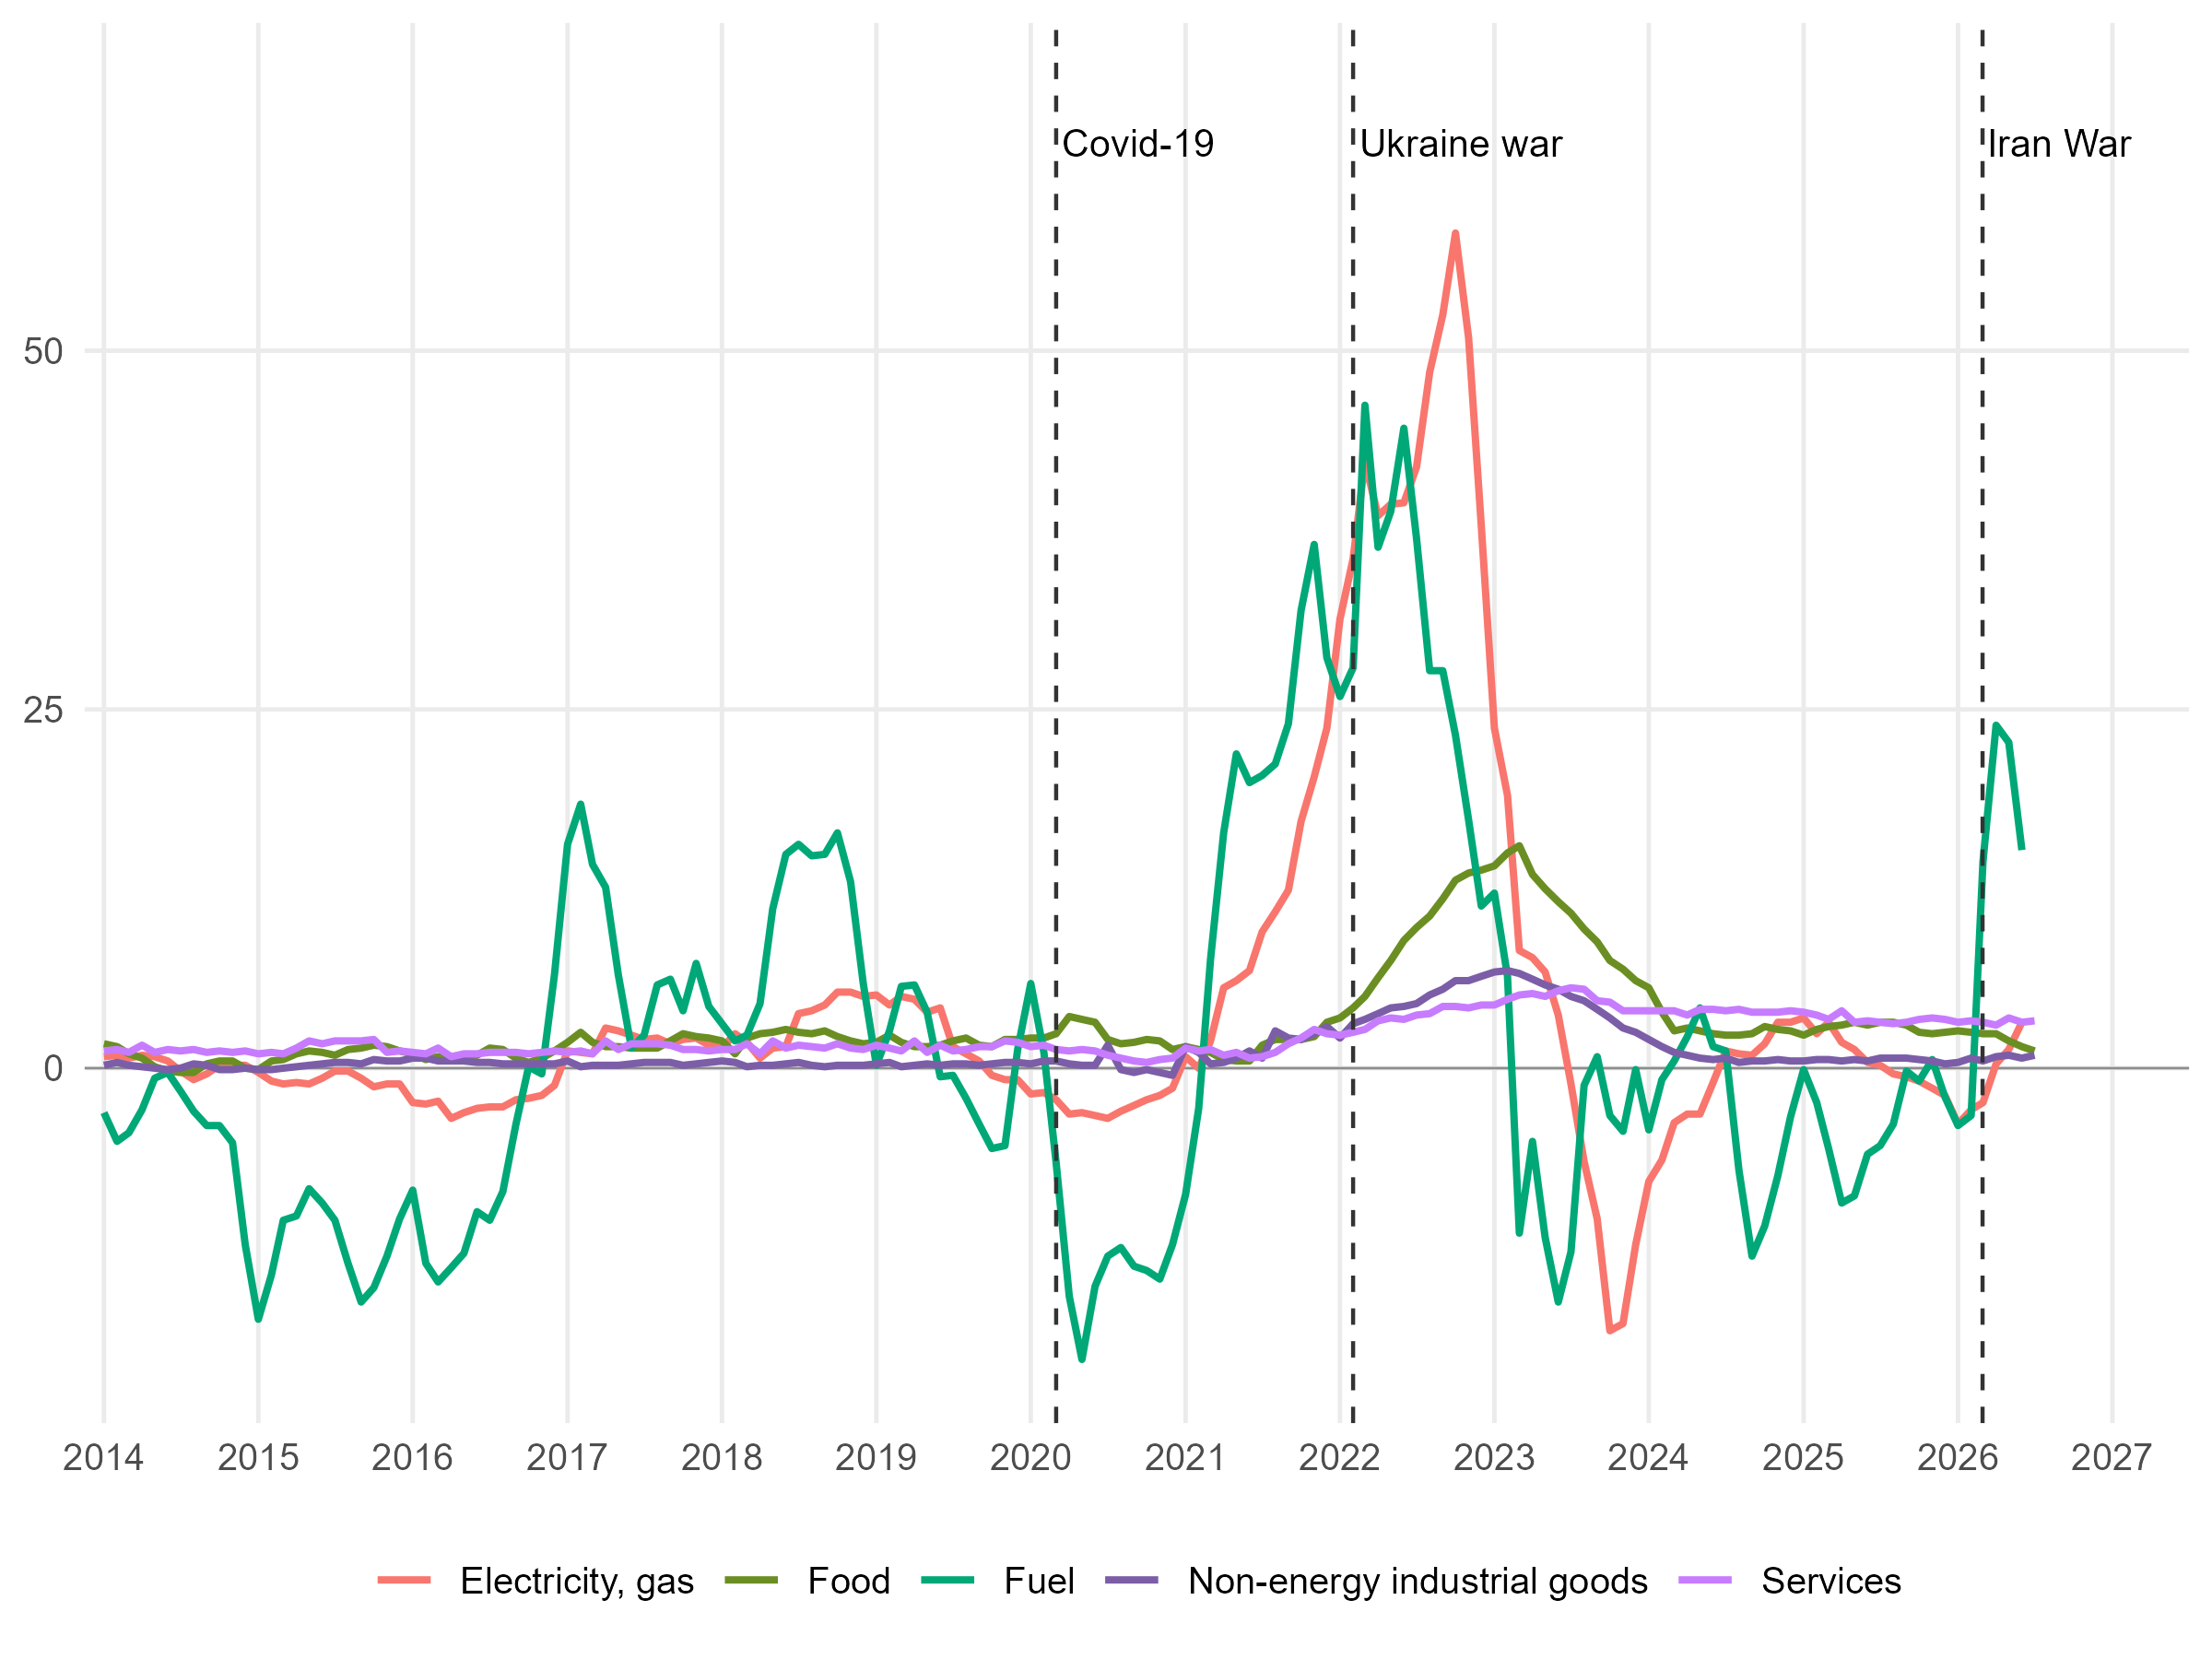
\includegraphics[scale=0.6]{fig/fig_EA_2014_2026_hicp_components.png}
\label{fig:hicp}
\captionsetup{font=footnotesize, format=hang, singlelinecheck=false, justification=justified}
\caption*{%Notes:\\ 
Source: Eurostat HICP euro-area aggregate, authors' calculations}
\end{figure}
%%%%%%%%%%%%%%%%%%%%%%%%%%%%%%%%%%%%%%%%%%%%%%%%%%%%%%%%%%%%%%



\subsection*{Consumption Data and Harmonisation Challenges}

The heterogeneity of consumption patterns among households is well-documented, but the accurate measurement of household-level consumption continues to present significant challenges. Estimating HICP inflation by household category therefore requires Household Budget Surveys (HBS), which are national surveys on consumer expenditure and household characteristics.

The Household Budget Surveys (HBS) are conducted on a large sample of households in each euro area country. Households are required to document their expenditures on consumer goods and services over a designated period, typically two weeks. These surveys capture the values of expenditures across COICOP categories. HBS data are generally collected every five years. The most recent and complete HBS wave generally took place in 2020. The 2020 HBS wave was actually conducted between 2018 and 2022 in most EU Member States, with a few country-specific timing exceptions.\footnote{The following HBS wave is the 2025 wave, with increased harmonization between countries.} A few national statistical institutes also provide higher-frequency HBS data that can be used for country-specific extensions.

Repeated HBS waves available for a subset of countries suggest that, while behavioural changes over the course of a few years can be significant, percentage-point differences in the weights of the main consumption categories between low- and high-income households remain relatively stable. This is the dimension that matters most for our estimates. Despite changes in overall consumption patterns, the impact of recent behavioural changes on inflation inequality may therefore be limited, since consumption shares often move in the same direction for different income groups.

%%%%%%%%%%%%%%%%%%%%%%%%%%%%%%%%%%%%%%%%%%%%%%%%%%%%%%%%%%%%%%
\begin{figure}[H]
\centering
\caption{Consumption baskets by income quintiles in the euro area (in \% of total expenditures)}
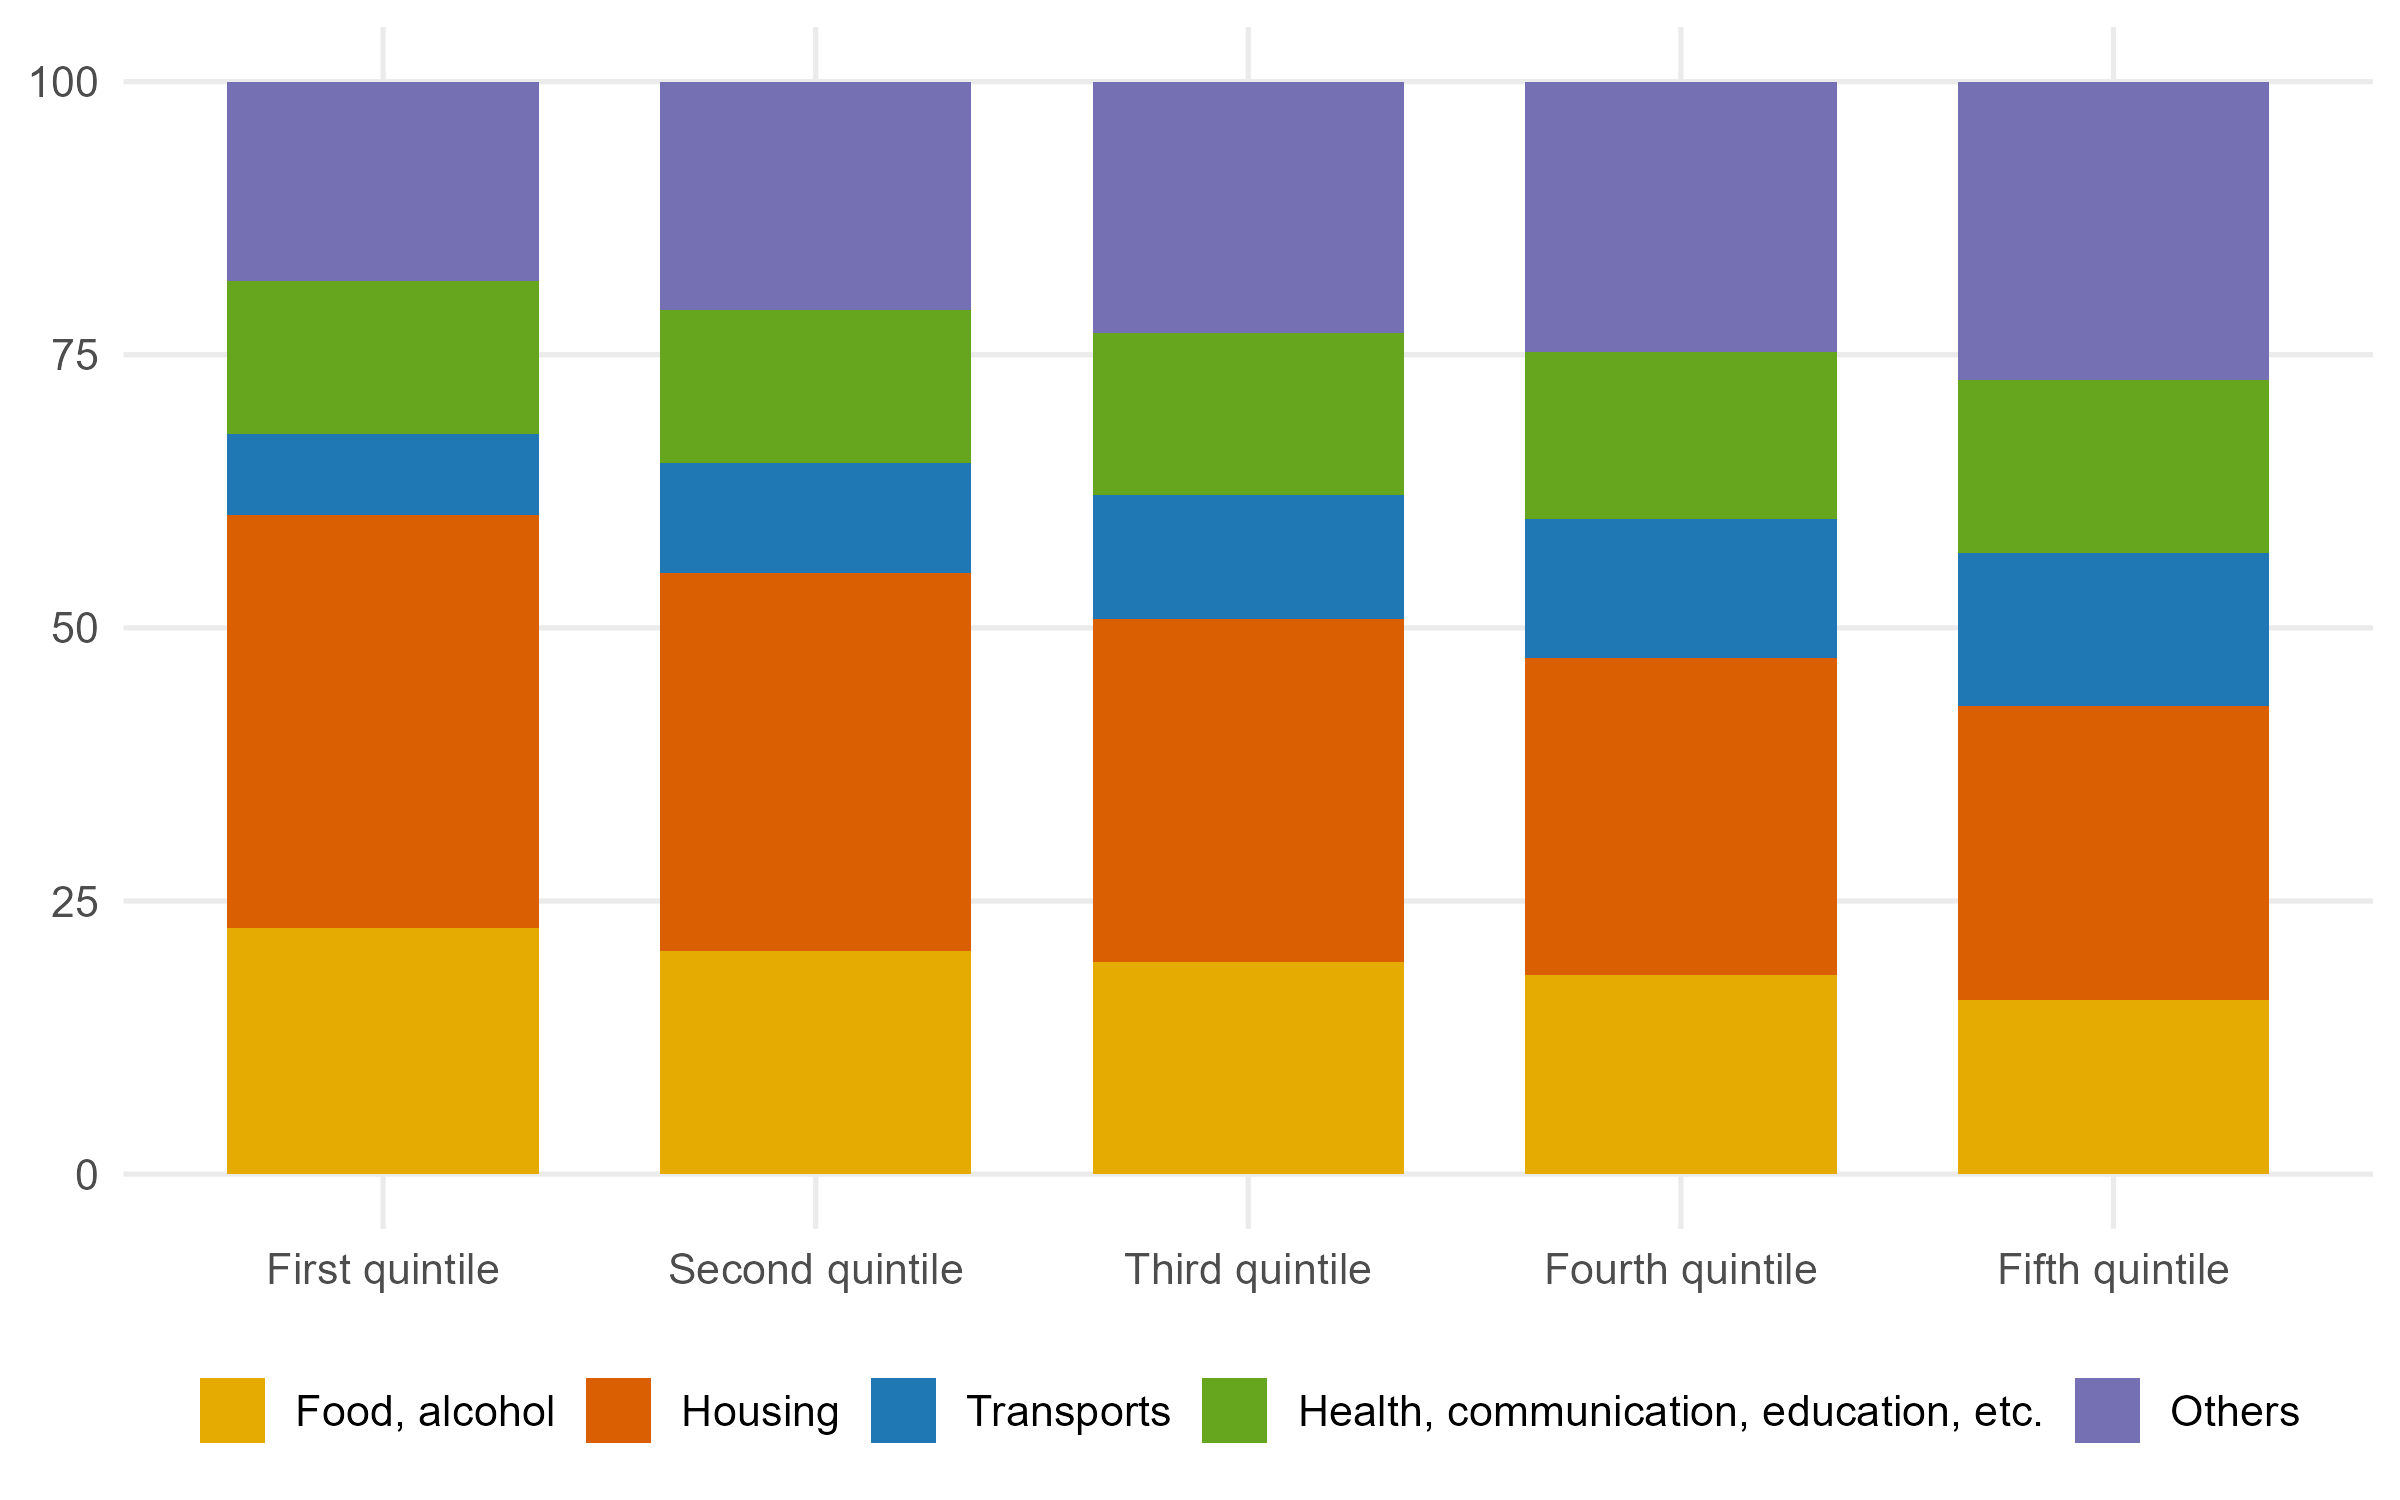
\includegraphics[width=0.86\textwidth,height=0.36\textheight,keepaspectratio]{fig/fig_EA_2020_income_consumption_baskets.png}
\label{fig:hbs}
\captionsetup{font=footnotesize, format=hang, singlelinecheck=false, justification=justified}
\caption*{Notes: Structure of consumption expenditure by income quintile.
The euro-area aggregate is computed from the 2020 HBS wave as the unweighted sum
of available country-level income-quintile expenditures, renormalised to 100
within each quintile. Countries without available HBS data for the wave are not
included in the aggregate. Italy is taken from the Eurostat HBS income-quintile
 table when available and from national HBS inputs otherwise.\\
Source: Eurostat HBS 2020, authors' calculations}
\end{figure}
%%%%%%%%%%%%%%%%%%%%%%%%%%%%%%%%%%%%%%%%%%%%%%%%%%%%%%%%%%%%%%


%This infrequent collection may not fully capture short-term fluctuations in consumption patterns, particularly during periods of rapid price changes (e.g. COVID-19), potentially leading to bias in inflation inequality during such periods.\footnote{\cite{accardo2023measuring} developed a methodology to address the issue of low-frequency data in household consumption surveys.} Significant changes in weights between successive waves of HBS can also result in abrupt variations in inflation estimates by category. To address this, a linear interpolation method is proposed to smooth variations.\footnote{To mitigate this issue, two approaches are available in the package: linearly interpolate the HBS weights to smooth out the changes in weights over time, or apply a specific year's HBS weights for all months when calculating inflation rates (or contributions to inflation).}
While HBS expenditure shares are observed only at low frequency, our weighting approach combines household-specific HBS expenditure structures with monthly HICP inflation rates. As a result, the average consumption trend can evolve continuously over the business cycle, reflecting changes in the HICP. However, because cross-household expenditure heterogeneity is assumed to remain constant between two HBS waves, a linear interpolation method is proposed to smooth variations at a specific date.


Figure~\ref{fig:hbs} presents the consumption baskets by income quintiles, revealing the disparities in expenditure patterns across different income groups. Notably, lower-income households allocate a larger proportion of their expenditure to essential goods such as food and energy, making them more vulnerable to price shocks in these categories.  Housing and food account for a substantially larger share of expenditure among lower-income households. Energy-related expenditure for housing and private transport is also much higher in rural areas than in cities, reflecting differences in heating needs and mobility constraints.


HICP and HBS are not designed to fit together mechanically. HICP item weights are updated every year and may rely on national accounts or other national sources, while HBS expenditure structures are observed at lower frequency. Depending on the level of data available, HICP and HBS are therefore merged at 3-digit COICOP in each country. In some cases, data published directly by national statistical institutes can be used instead of relying only on the Eurostat dataset. This approach is particularly valuable when the nationally published data provide greater granularity, recency, or frequency.\footnote{The \texttt{inflationinequality} R package allows the use of national data at 4-digit COICOP.}

The HBS contains many household characteristics that can be used to segment inflation exposure. In this paper, we focus on three dimensions that are both economically meaningful and widely available across countries: income, the age of the household reference person, and the area of residence.\footnote{In recent HBS waves, Eurostat generally requests the Degree of Urbanisation (DEGURBA) variable, built from a common European methodology based on a 1 km$^2$ population grid. It classifies residence areas into cities (densely populated areas), towns and suburbs (intermediate density areas), and rural areas (thinly populated areas), using comparable thresholds across EU countries: urban centres of at least 50,000 inhabitants and 1,500 inhabitants per km$^2$, urban clusters of at least 5,000 inhabitants and 300 inhabitants per km$^2$, and all remaining areas.} These variables make it possible to compare inflation experiences not only across the income distribution, but also across demographic groups and territorial contexts. In line with the Eurostat HICP methodology, imputed rent is excluded from the analysis. This analysis uses all available waves of the HBS since 1999 and matches them with the closest corresponding HICP year. Country-specific extensions based on national HBS microdata are described in the appendices when harmonised Eurostat inputs are incomplete for the required household breakdowns.


%The Consumer Price Index (CPI) and Household Budget Surveys (HBS) are categorized according to the COICOP nomenclature. However, the relationship between the COICOP-CPI and COICOP-HBS classifications is not bijective. To address this, all CPI items are retained while expenditures from the HBS that fall outside the scope of consumption--such as taxes and work-related investment expenditures--are excluded. 

% Adjustments are made to the nomenclature for items that lack direct correspondence or are categorized differently. Where feasible, matching is conducted at level 3 of the COICOP consumption function nomenclature, and at level 2 where finer disaggregation is unavailable (e.g., transport services, where modal breakdowns are absent in the HBS), ensuring the inclusion of all CPI products.

%We explain the harmonized methodology applied across all euro area countries, utilizing an R package. The average of inflation measures by categories equals average inflation (cf. Jaravel?). The package allows the use of custom national data where available. 
These data constraints motivate the weighting methodology below. A simple use of HBS expenditure shares would generally not aggregate back to the official HICP, because the HBS all-household basket does not necessarily coincide with the annually updated HICP item weights. We therefore start from the official HICP product weights and use HBS only to distribute each product's expenditure across household groups. The RAS (Row and Column Adjustment Scaling) calibration preserves the relative HBS expenditure profiles while imposing the row and column margins required by the HICP construction.

\subsection*{Group-Specific Weights}

Let $\omega^{HICP}_{j,y}$ denote the official annual HICP weight of product
category $j$ in weight year $y$. Let $g$ denote a household group, such as an
income quintile, an age group, or a residence-area group. The HBS correction
factor is defined as:

\begin{equation}
c^{HBS}_{j,g,y'}
=
\frac{E^{HBS}_{j,g,y'}}{E^{HBS}_{j,\mathrm{all},y'}},
\end{equation}

where $E^{HBS}_{j,g,y'}$ is HBS expenditure on product category $j$ by group
$g$ in HBS wave $y'$, and $E^{HBS}_{j,\mathrm{all},y'}$ is the corresponding
expenditure for all households. $E^{HBS}_{g,y'}$ and
$E^{HBS}_{\mathrm{all},y'}$ denote total HBS consumption expenditure by group
$g$ and by all households, respectively. The coefficient $c^{HBS}_{j,g,y'}$
therefore measures the share of aggregate HBS expenditure on product $j$
accounted for by group $g$.


The weights $\omega_{j,g,y}$ are obtained from the RAS calibration. The algorithm preserves the
relative HBS expenditure profiles while making the expenditure-weighted average
of group baskets reproduce the official HICP item weights. Appendix
\ref{sec:app-weight-normalization} describes the RAS algorithm and compares it
with the relative-expenditure normalization.

The calibrated
aggregate expenditure matrix $M_{j,g,y}$ is required to satisfy the original
HICP item-weight margins. Let $s_{g,y}$ denote the share of total household
consumption expenditure accounted for by group $g$ in weight year $y$:
\begin{equation}
s_{g,y}
=
\frac{E^{HBS}_{g,y'}}{\sum_h E^{HBS}_{h,y'}}.
\end{equation}
The RAS calibration imposes:
\begin{equation}
\sum_{j \in \mathcal{J}_y} M_{j,g,y}
=
s_{g,y}\sum_{j \in \mathcal{J}_y}\omega^{HICP}_{j,y}
\quad \text{for all } g,
\qquad
\sum_g M_{j,g,y}
=
\omega^{HICP}_{j,y}
\quad \text{for all } j.
\end{equation}
The product margin, $\sum_g M_{j,g,y}=\omega^{HICP}_{j,y}$, ensures that the
expenditure-weighted average of the group-specific weight assigned to each
product reproduces the official HICP weight for that product. The group margin,
$\sum_{j \in \mathcal{J}_y} M_{j,g,y}$, fixes the total expenditure mass of
each household group, so that groups can retain different product structures
while aggregating back to the published HICP basket.
The final group-specific HICP weight is obtained by normalizing the calibrated
matrix within each group:
\begin{equation}
\omega_{j,g,y}
=
\frac{M_{j,g,y}}{\sum_{k \in \mathcal{J}_y}M_{k,g,y}}.
\end{equation}

After aggregation, this calibration closely reproduces the official inflation
rate (see Appendix~\ref{sec:app-weight-normalization}), and validation checks
are reported in Appendix~\ref{sec:app-validation-tests}.


We use the Household Budget Survey as released by Eurostat once every five years. In
contrast, the expenditure weights used in the construction of the HICP are
updated annually. The year of the HBS data $y'$ and the HICP weight year $y$
may therefore differ. To align the two sources, each HICP weight year $y$ is
matched with the most recent HBS wave available at or before that year. If no
earlier HBS wave is available, the earliest HBS wave is used.

As a rule, HICP data are available on Eurostat at a level of detail
corresponding to the 5-digit COICOP classification. However, certain product
categories lack price data for specific periods. For instance, early-year
price data for medical consultation services ("062") is often unavailable. To
address these gaps, missing price indices are estimated based on the price
developments of their parent product categories. In the case of "062", the
price movements of the broader "health services" category ("06") are used to
estimate the missing data.

\subsection*{Group-level Consumer Price Indices}

Let $p_{j,y,m}$ denote the Laspeyres price index of product category $j$ in month
$m$ of year $y$. Let $p_{j,y,0}$ denote the price reference used for the HICP
weight year $y$; in the chained annual calculation this corresponds to the
December price index of the previous year. The aggregation procedure is as follows: item indices are first unchained within the
weight year, aggregated with annual expenditure weights, and then chained
again.\footnote{See Eurostat's \texttt{hicp} R package, which implements the
Eurostat HICP aggregation.}
The group-specific within-year price index therefore combines unchained product
indices with the group-specific weights defined above:

\begin{equation}
P_{g,y,m}
=
\sum_{j \in \mathcal{J}_y}
\omega_{j,g,y}
\cdot
\frac{p_{j,y,m}}{p_{j,y,0}}.
\end{equation}

The chained price index for household group $g$, denoted $I_{g,y,m}$, is then
obtained by linking each within-year index to the previous December:

\begin{equation}
I_{g,y,m}
=
I_{g,y-1,12}
\cdot
P_{g,y,m}.
\end{equation}

This notation keeps the two objects distinct: $\omega_{j,g,y}$ is the annual
group-specific HICP weight of product $j$, while $I_{g,y,m}$ is the resulting
monthly chained price index for group $g$. Because chained indices are not
additive, product-level contributions do not mechanically sum to the aggregate
year-on-year inflation rate unless the contribution formula accounts for the
chain-linking structure.


%The HICP data is available on Eurostat at a minimum level of detail corresponding to the 2-digit COICOP classification.

%HICP weights, adjusted each year. HICP weights are used to normalise consumption structures so that aggregation of the indices by category produces the HICP.


%In contrast, essential expenditures, such as housing, food, healthcare, and transportation, constitute almost two-thirds of total consumption for lower-income households, compared to less than half for higher-income households. 

\section{Main Results}
\label{sec:main-results}

This section presents our main results. We focus on inflation inequality in the wake of the 2022--23 energy crisis and also document long-run inflation inequality in the euro area.



\subsection{Euro Area}

%We first describe patterns of inflation inequality over the short run since 2020. 

\subsubsection{Short-Run Inflation Inequality}

%Euro area results indicate small or large differences across categories. We also examine product contributions to inflation inequalities. 

%We find a smaller amount of inflation inequality than the ECB during the past inflationary episode within the euro area.  The differences primarily stem from our distinct aggregation procedure, which accounts for country-specific consumption patterns with more granularity. This methodological choice reflects our emphasis on capturing national idiosyncrasies in both consumption patterns and price dynamics.


%In 2022, the contributions of different product categories to the inflation gap (between low and high-income households) tended to cancel each other out (e.g., energy prices vs. services). However, in 2023, rising food prices disproportionately affected low-income households, increasing the inflation gap (Figure 3).

Figure~\ref{fig:ea20_short_run_income} shows that the post-COVID inflation
surge did not translate into marked inflation inequality by income quintile
at the euro-area aggregate level. Inflation rates for the first and fifth
income quintiles move closely together throughout the 2020--2026 period. Energy
and food shocks raised headline inflation sharply, but their effects on the
relative inflation exposure of low- and high-income households largely offset
once national consumption structures and country-level price dynamics are
combined at the euro-area level.

%%%%%%%%%%%%%%%%%%%%%%%%%%%%%%%%%%%%%%%%%%%%%%%%%%%%%%%%%%%%%%
\begin{figure}[H]
\centering
\caption{Short-run inflation inequality in the euro area by income quintile (in \%)}
\label{fig:ea20_short_run_income}
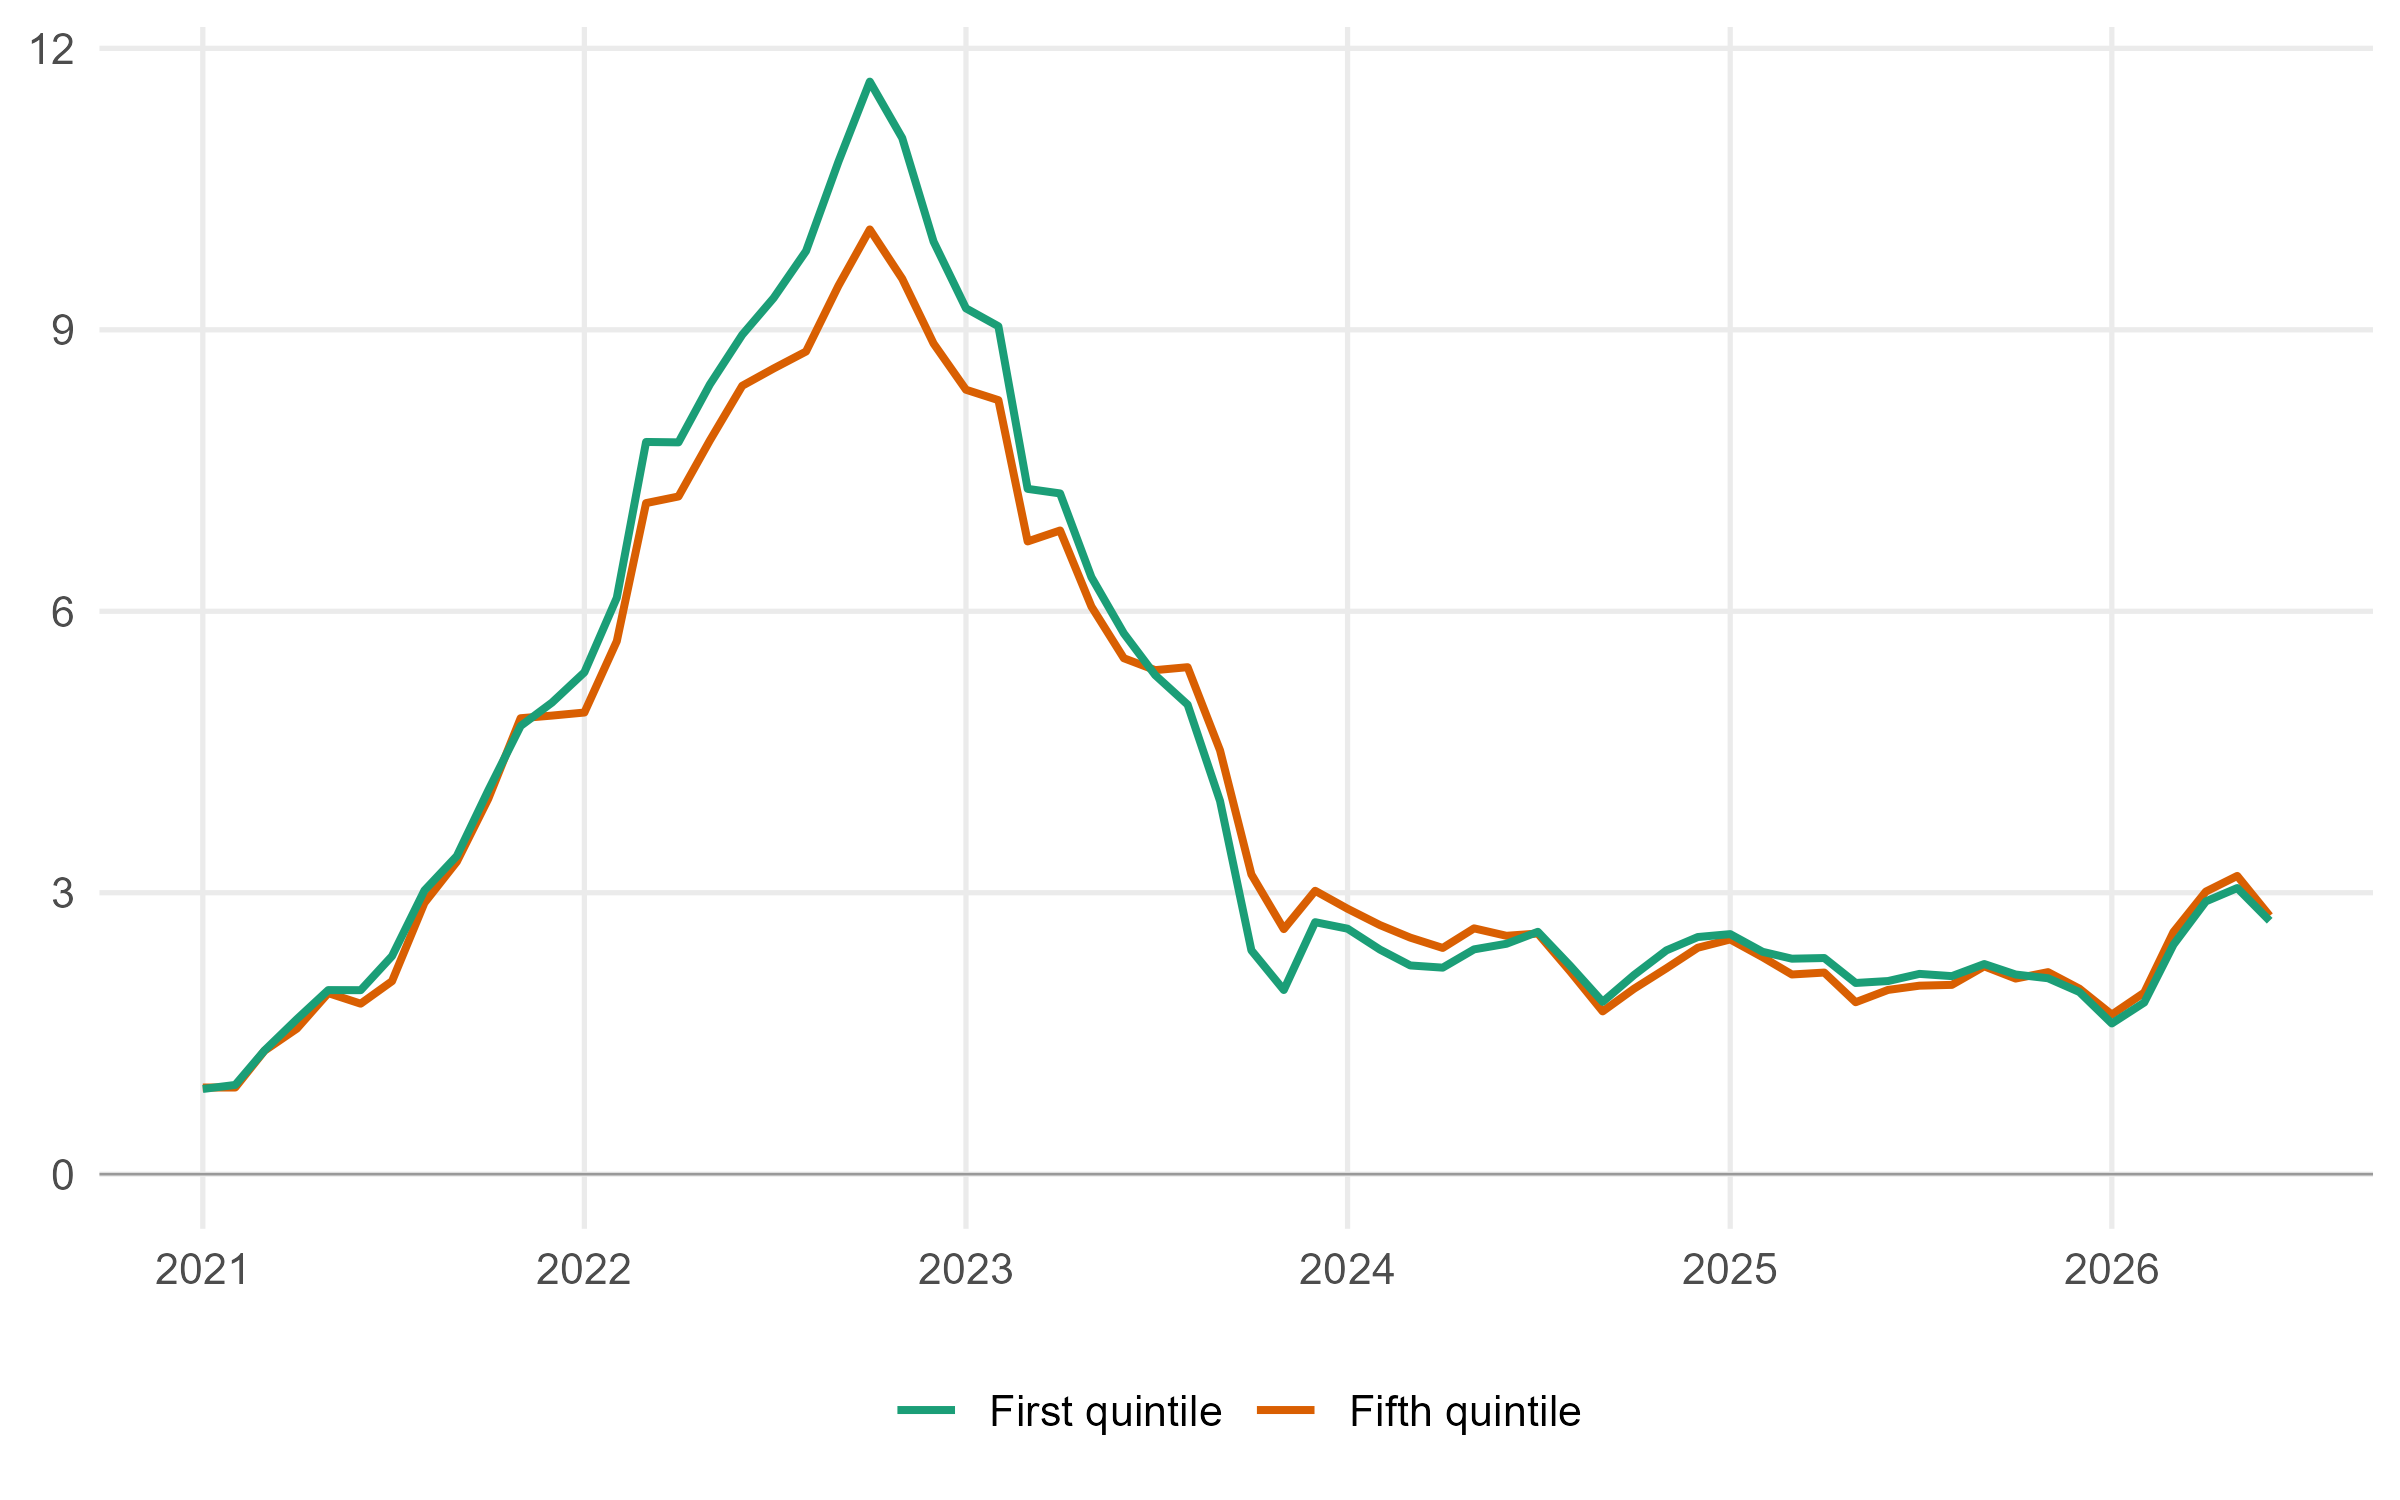
\includegraphics[scale=0.6]{fig/fig_EA20_2020_2026_income_inflation_Q1_Q5.png}
\vspace{6pt} 
\captionsetup{font=footnotesize, format=hang, singlelinecheck=false, justification=justified}
\caption*{Note: This figure reports year-on-year inflation rates for the first and fifth income quintiles in the euro area, January 2020 to April 2026.\\
Sources: Eurostat HICP, HBS, authors' calculations}
\end{figure}
%%%%%%%%%%%%%%%%%%%%%%%%%%%%%%%%%%%%%%%%%%%%%%%%%%%%%%%%%%%%%%
\newpage


\subsubsection{Inflation Inequalities by Age and Residence Areas}

%Papers on inflation inequality focus on inequality according to household income brackets. However, in the case of most countries, it was inflation differentials between age groups or residence areas that were much more pronounced during the 2021-2023 period.

Figure~\ref{fig:age_rural} presents inflation rates by household category in the euro area, segmented by age and residence area. Panel (a) shows inflation disparities by age, with older households experiencing higher inflation rates because they spend more on essential goods. Panel (b) highlights differences by residence area, with rural households facing higher inflation rates than households living in cities.

The residence-area differentials are consistent with differences in the structure of energy demand. Rural households tend to spend a larger share of their budget on transport fuels and home energy, partly because commuting distances are longer and the set of available transport substitutes is more limited. During an energy-price shock, these structural features translate into larger short-run inflation exposure.

%%%%%%%%%%%%%%%%%%%%%%%%%%%%%%%%%%%%%%%%%%%%%%%%%%%%%%%%%%%%%%
\begin{figure}[H]
\centering
\caption{Inflation by household categories in the euro area (in \%)}
\label{fig:age_rural}
\begin{subfigure}{0.48\textwidth} 
  \centering
  \caption{By age}
  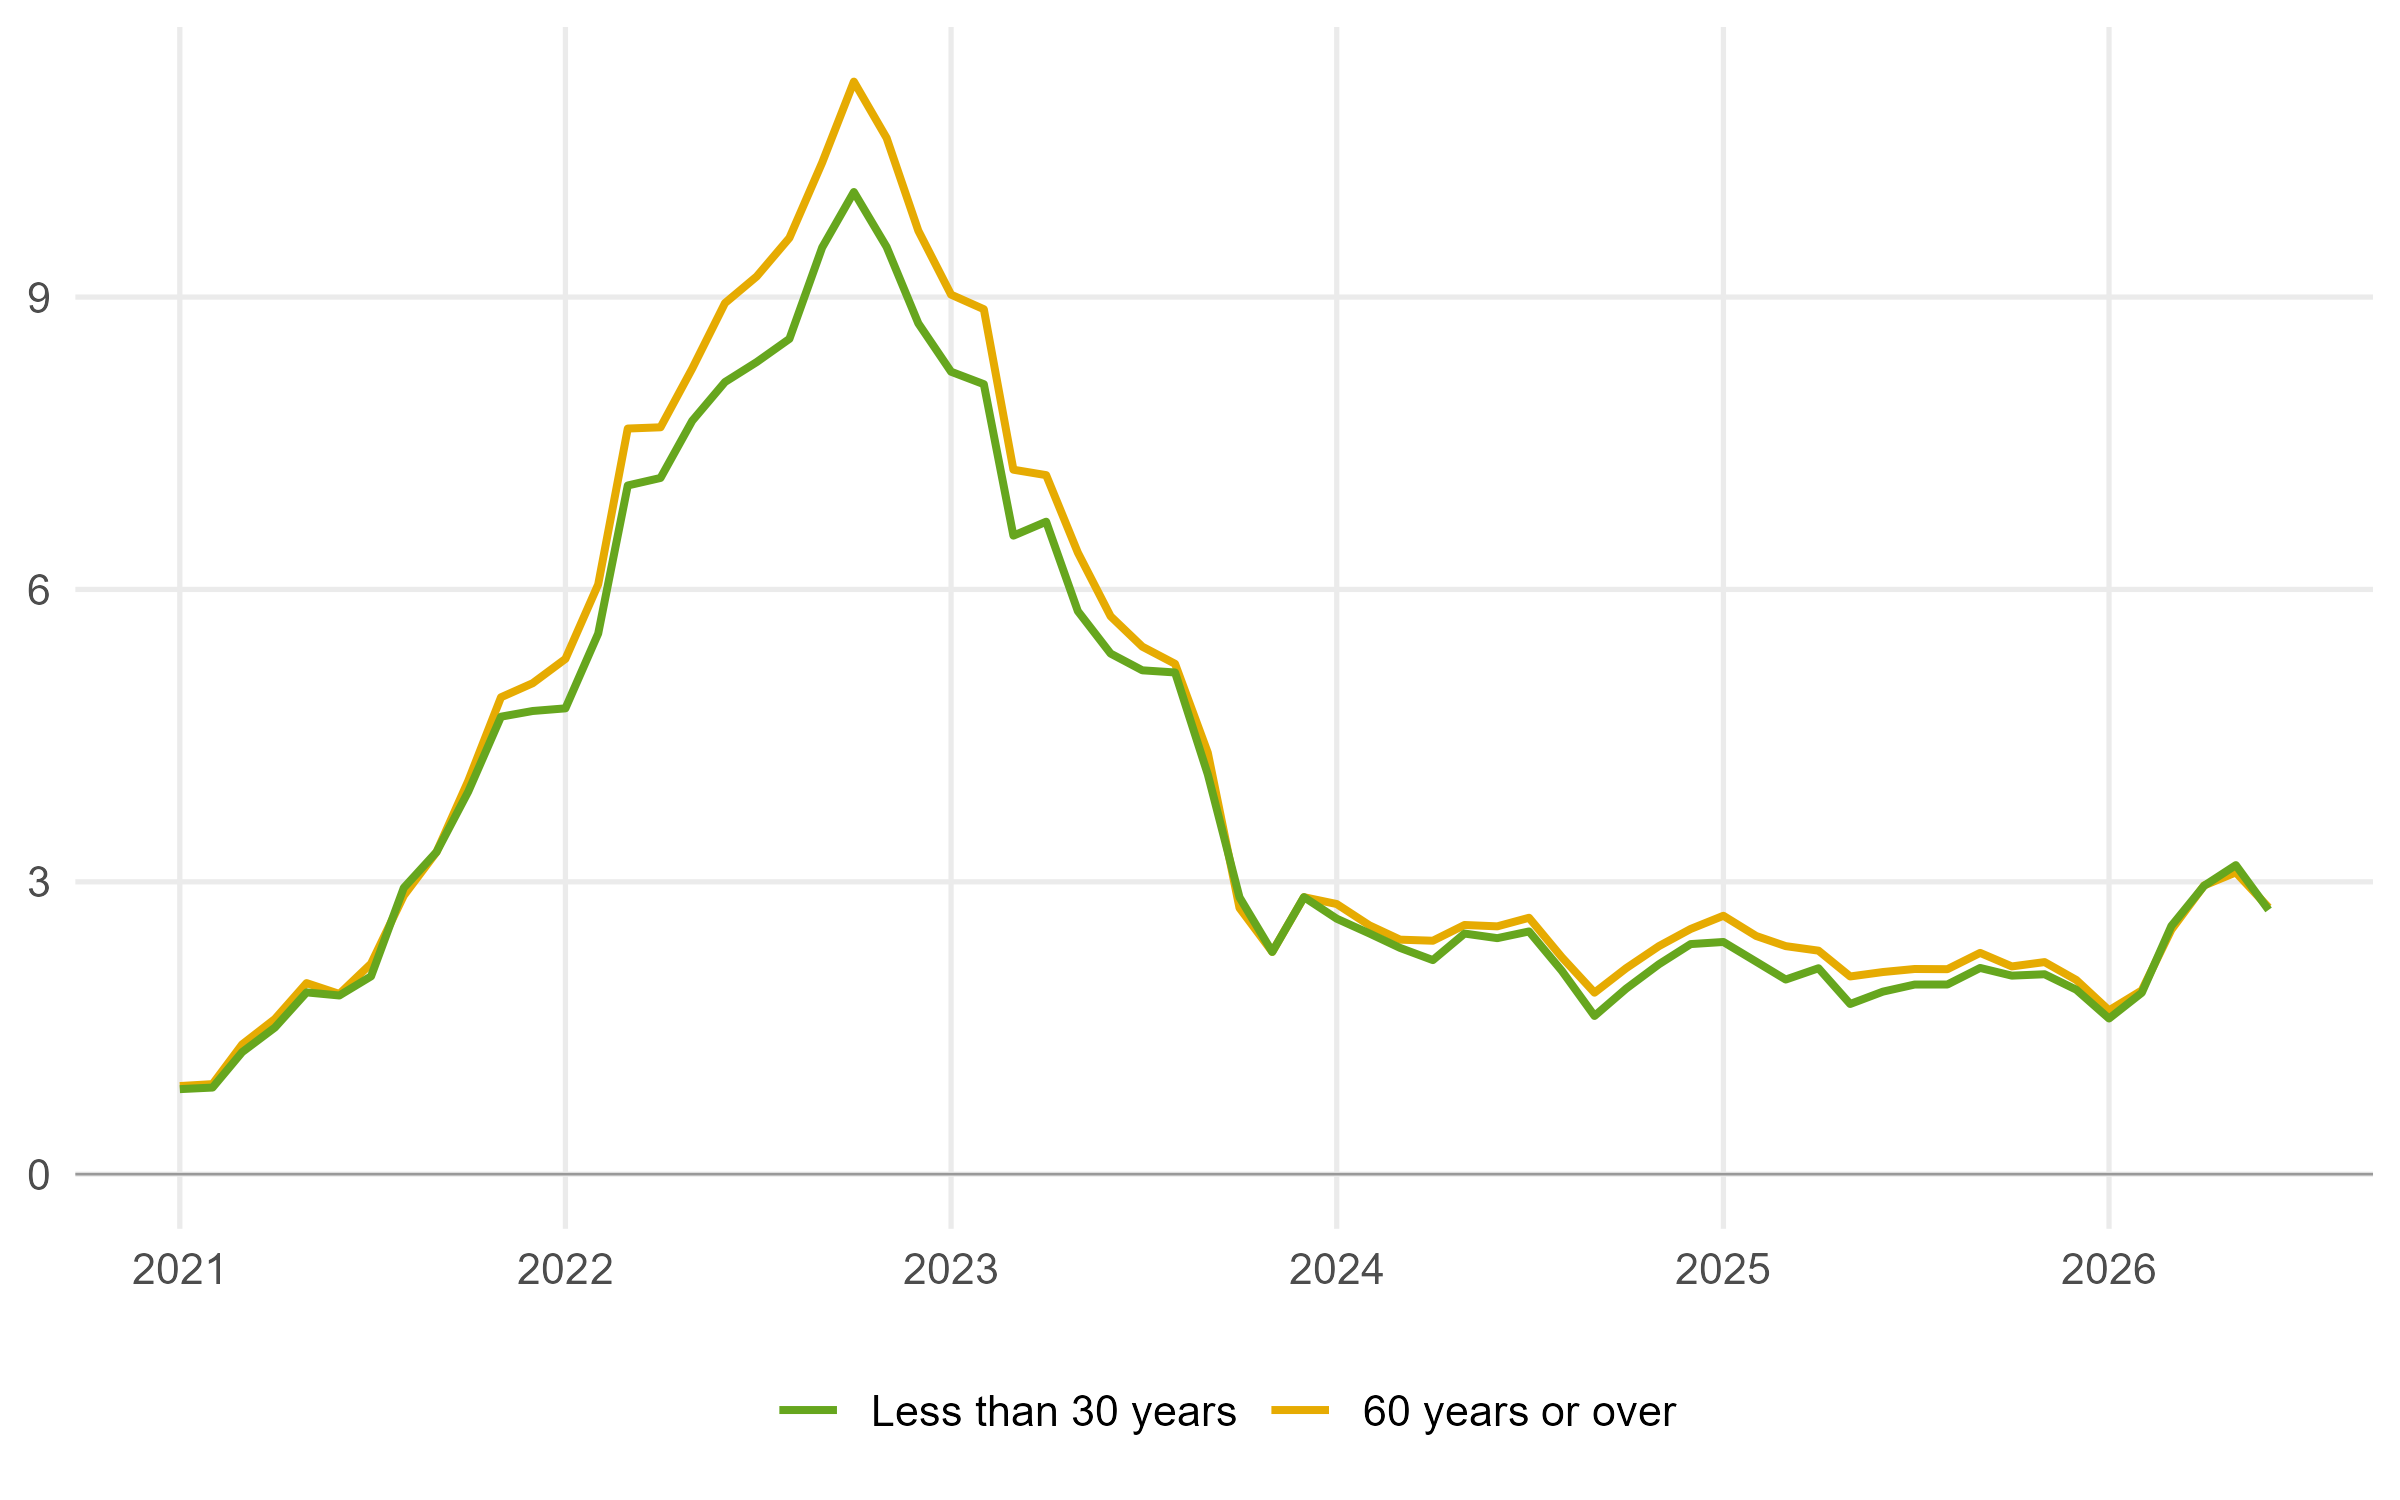
\includegraphics[width=\linewidth,height=6cm]{fig/fig_EA20_2020_2026_age_inflation_under30_60plus.png}
\end{subfigure}
\hfill 
\begin{subfigure}{0.48\textwidth} 
  \centering
  \caption{By residence area}
  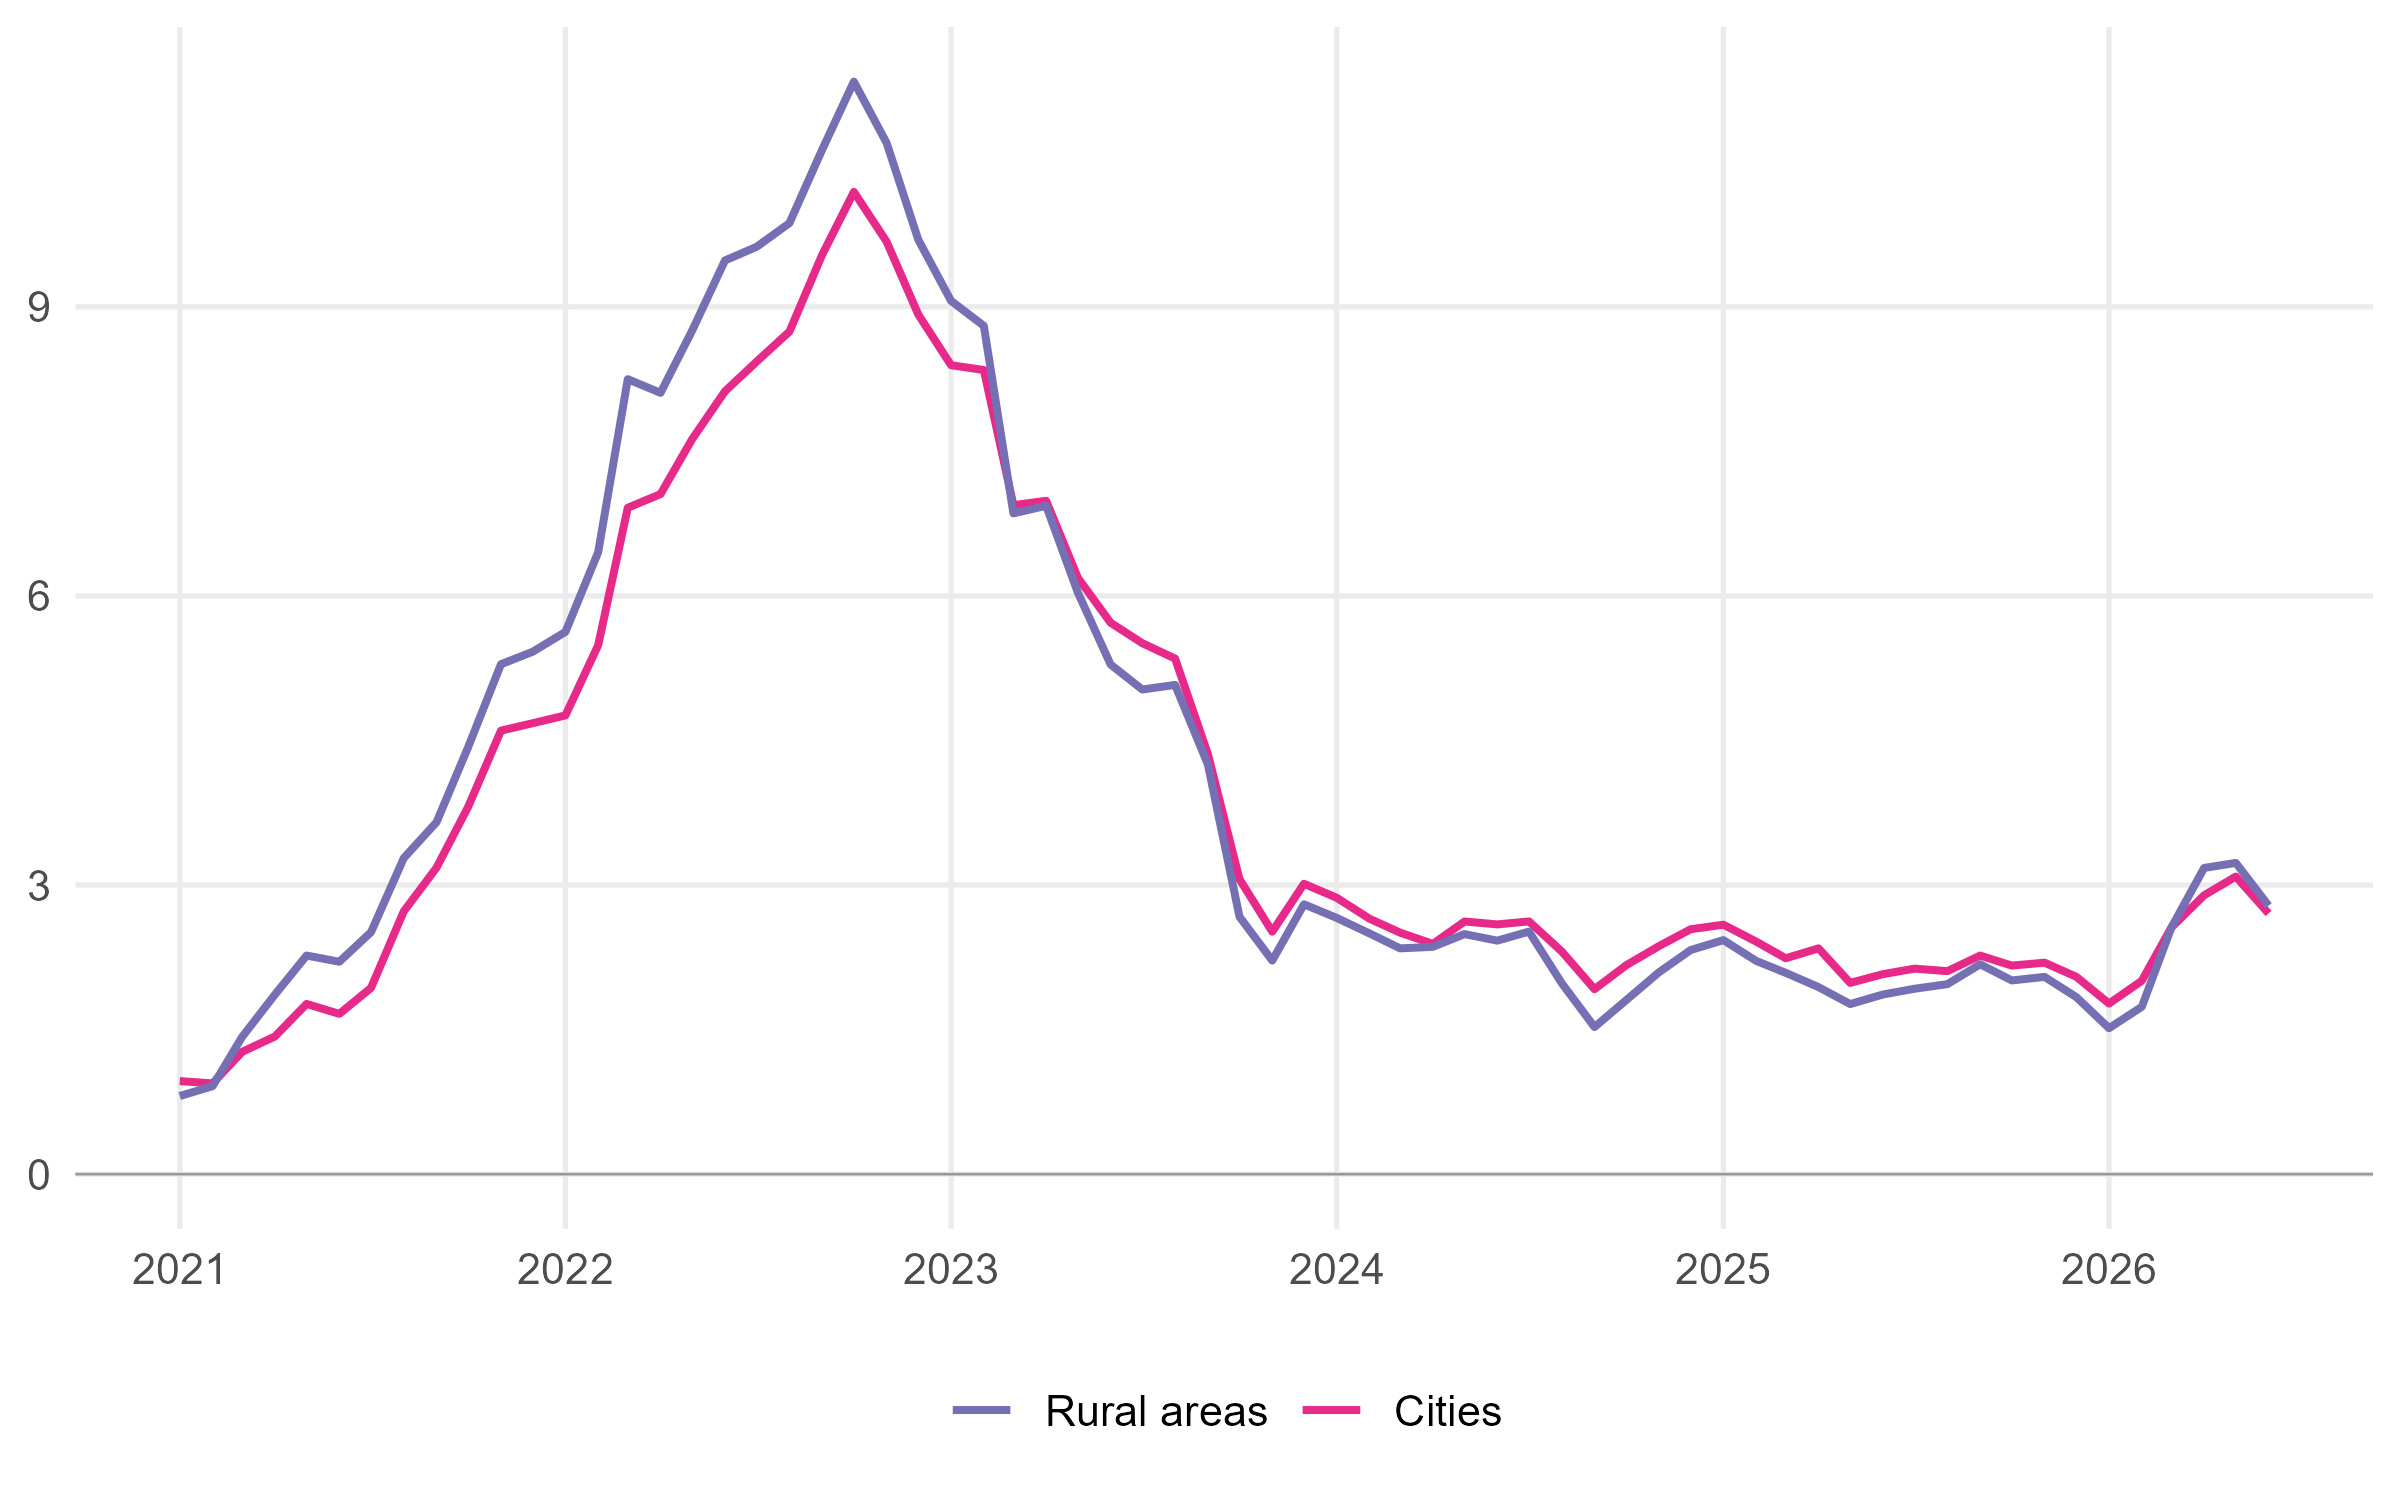
\includegraphics[width=\linewidth,height=6cm]{fig/fig_EA20_2020_2026_urban_inflation_rural_cities.png}
\end{subfigure}
%\label{fig:5}
\vspace{10pt} 
\captionsetup{font=footnotesize, format=hang, singlelinecheck=false, justification=justified}
\caption*{Note: This figure reports year-on-year inflation rates in the euro area by
age (panel a) and residence area (panel b), January 2020 to April 2026.\\
Sources: Eurostat HICP, HBS, authors' calculations}
\end{figure}
%%%%%%%%%%%%%%%%%%%%%%%%%%%%%%%%%%%%%%%%%%%%%%%%%%%%%%%%%%%%%%
\newpage




\subsubsection{Long-Run Inflation Inequality}


Figure~\ref{fig:ea20_long_run_income} depicts long-run inflation inequality in
the euro area by income quintile, showing price indices from January 2000 to
April 2026. The long-run evolution of price indices by income quintile reveals
persistent but modest divergences over time. The post-COVID inflation episode
is visible in the common increase in price levels after 2021, but it does not
generate a large cumulative inflation gap between the first and fifth income
quintiles at the euro-area aggregate level. This suggests that, once country
aggregation is taken into account, the recent inflation surge was primarily a
broad-based price-level shock rather than a strong source of income-based
inflation inequality for the euro area as a whole.

This pattern contrasts with the larger long-run gaps documented for the United
States in \cite{jaravel2024distributional}. Several differences may account for
this comparison. First, the euro-area indices reported here aggregate national
indices and therefore average across countries with different price dynamics
and fiscal responses. Second, the HICP-based calibration constrains
household-group baskets to aggregate back to the official euro-area price
index.

%%%%%%%%%%%%%%%%%%%%%%%%%%%%%%%%%%%%%%%%%%%%%%%%%%%%%%%%%%%%%%
\begin{figure}[H]
\centering
\caption{Long-run inflation inequality in the euro area by income quintile (index, 2000 = 100)}
\label{fig:ea20_long_run_income}
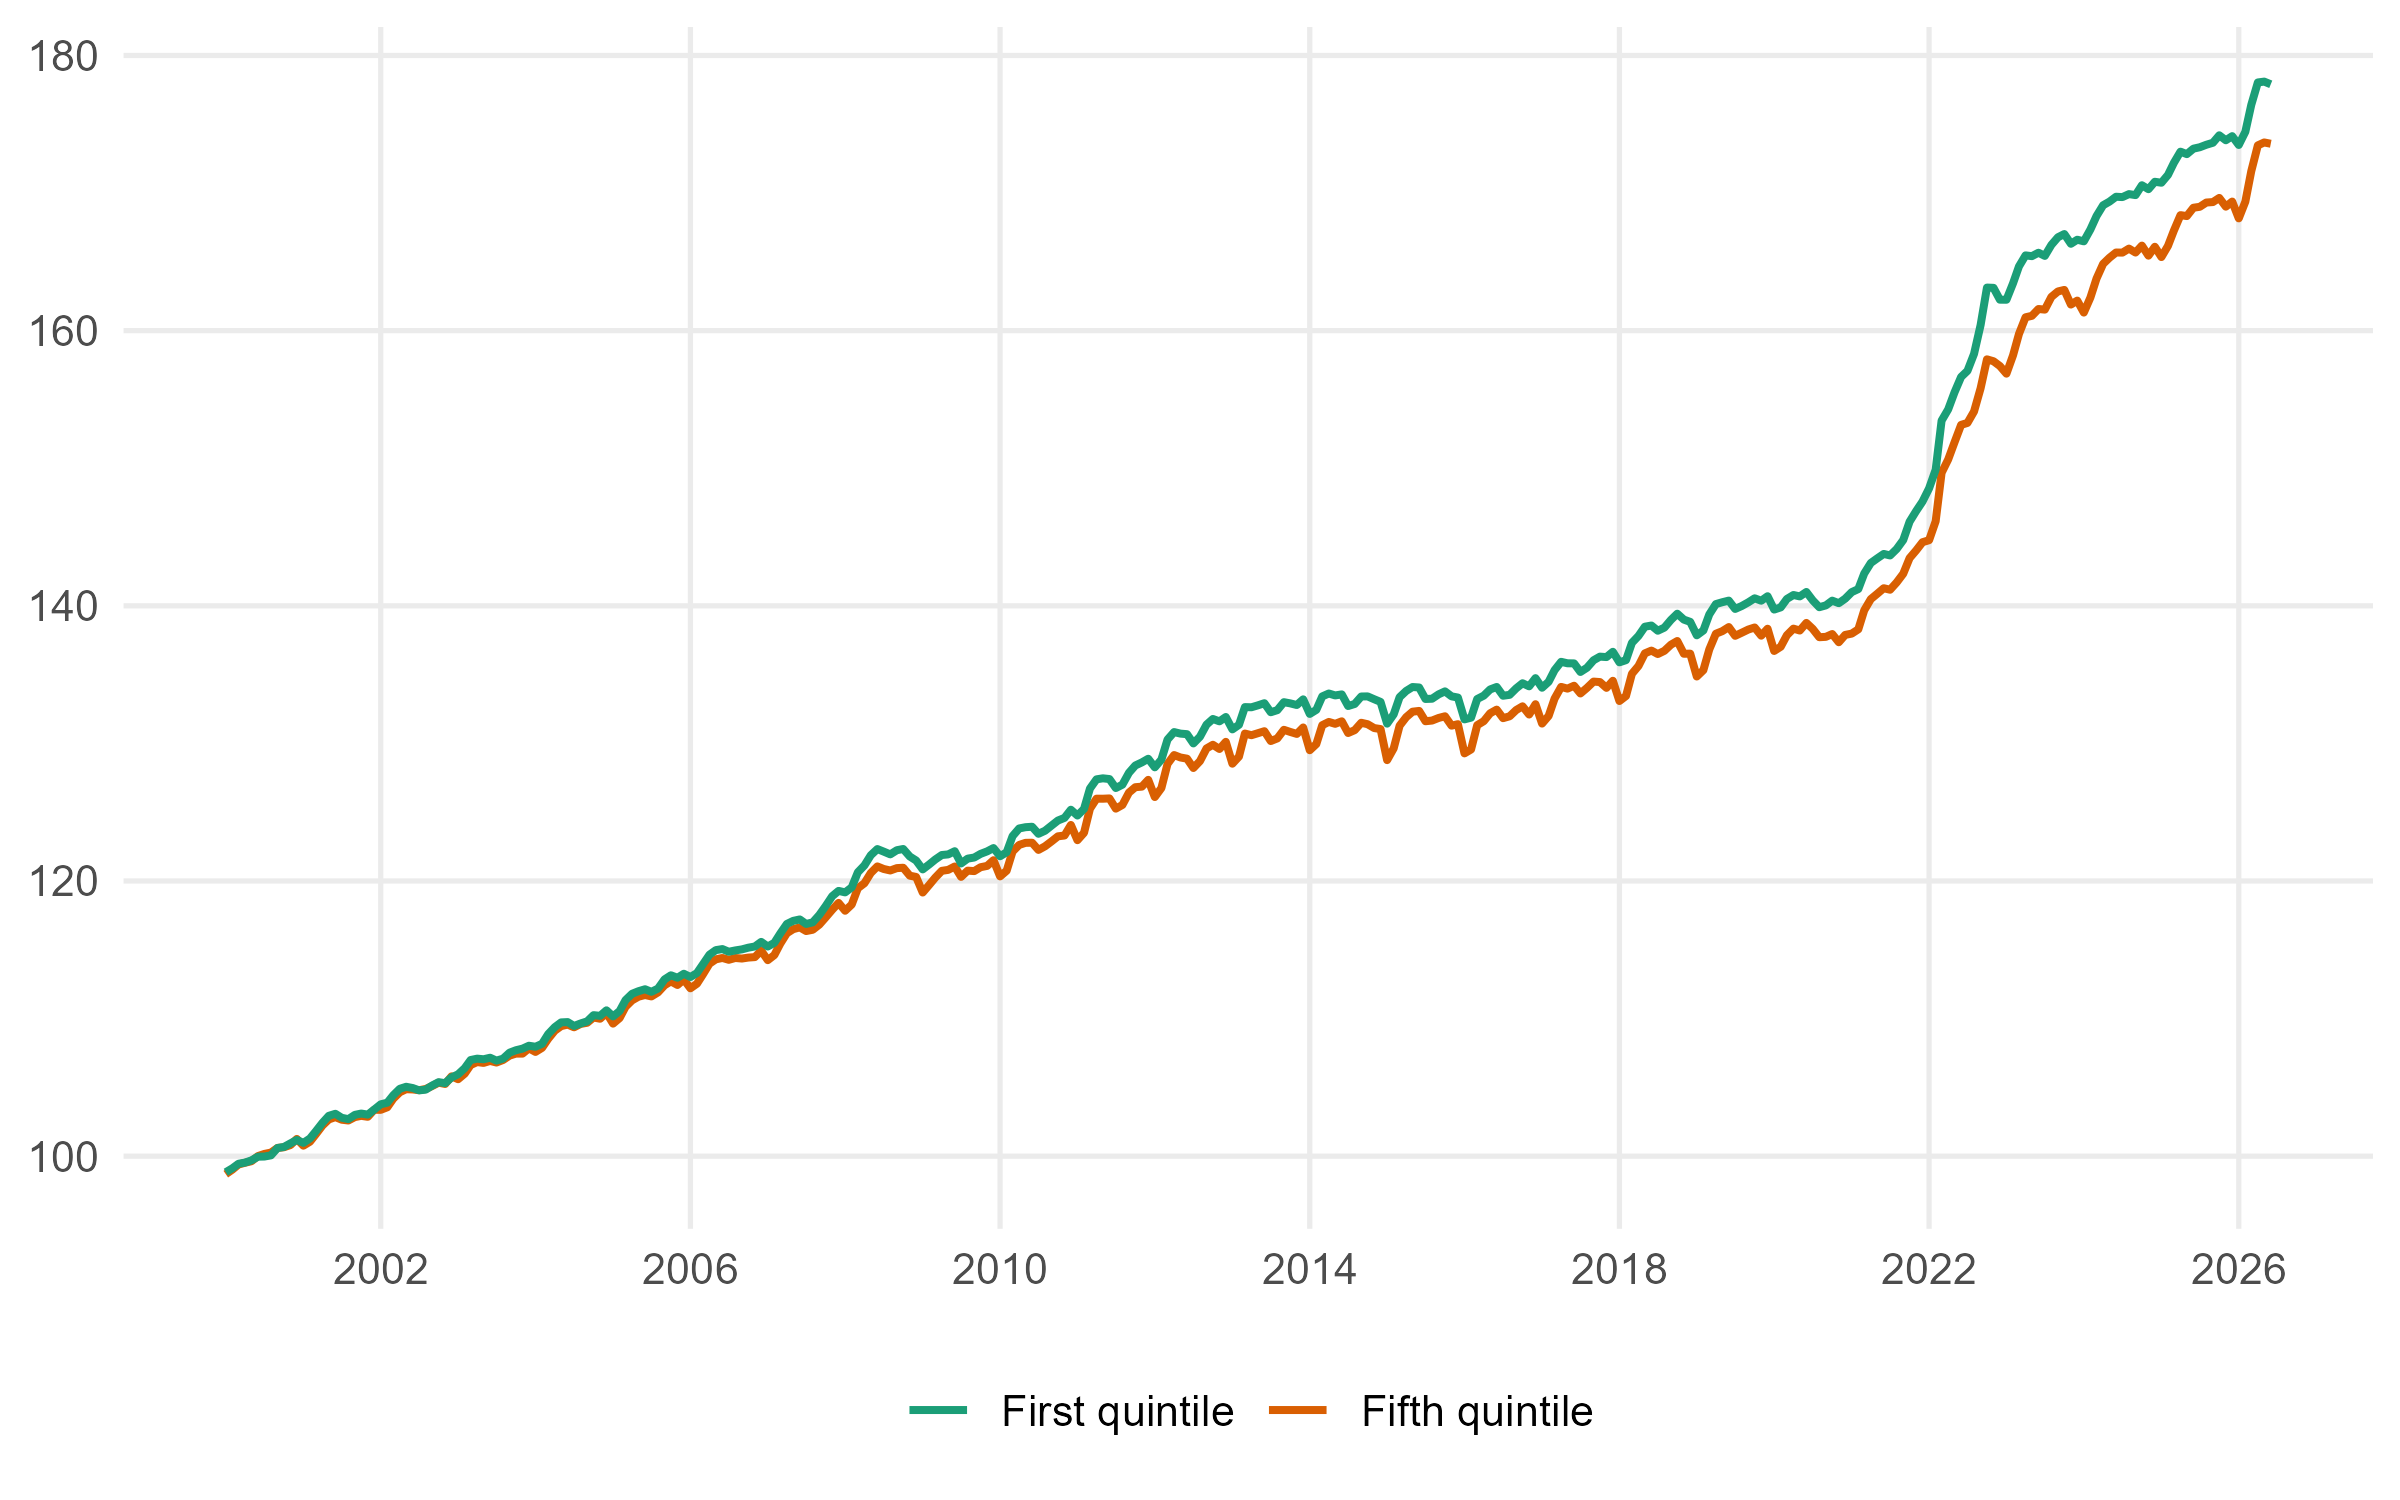
\includegraphics[width=0.82\textwidth,height=0.31\textheight,keepaspectratio]{fig/fig_EA20_2000_2026_income_price_index_Q1_Q5_base2000.png}
\vspace{6pt} 
\captionsetup{font=footnotesize, format=hang, singlelinecheck=false, justification=justified}
\caption*{Note: This figure shows monthly price indices for the first and fifth income quintiles in the euro area, January 2000 to April 2026. Indices are rebased to 2000 = 100.\\
Sources: Eurostat HICP, HBS, authors' calculations}
\end{figure}
%%%%%%%%%%%%%%%%%%%%%%%%%%%%%%%%%%%%%%%%%%%%%%%%%%%%%%%%%%%%%%
\newpage

%\cite{jaravel2021inflation} identifies two key factors explain the different consumption patterns of households. First, technological progress tend to disproportionately benefit higher-income households. Second, globalization has not provided significant compensatory benefits to lower-income households. Instead, its advantages have largely bypassed these groups, exacerbating existing disparities rather than mitigating.

\subsection{Heterogeneous Effects of the 2022--23 Energy Shock Across Countries}

%We observe heterogeneity in inflation inequalities across the euro area. Is there a link between inflation inequalities and inflation levels? 

%\subsection*{Four different Patterns of Inflation Inequality}

The 2022--23 inflation episode was marked by a large energy-price shock,
especially in gas markets, following Russia's invasion of Ukraine. Although this
shock was common to the euro area, its distributional effects differed across
countries because energy mixes, import dependence, household consumption
patterns, and fiscal responses were not uniform.

Table~\ref{tab:country-heterogeneity-cumulative-gap} documents this
cross-country heterogeneity by reporting the cumulative 2020--2024 inflation
gap between the first and fifth income quintiles. The Baltic countries and
Ireland display large positive Quintile 1--Quintile 5 gaps, while several large economies show
more compressed or slightly negative gaps despite substantial headline
inflation. This pattern is consistent with recent evidence on inflation
inequality in the euro area \citep{claeys2022inflation}. The sign and size of
inflation inequality are not mechanically tied to the level of inflation alone.

The relevant mechanism is the interaction between country-specific price
dynamics and group-specific expenditure shares. A price increase in a product
category generates inflation inequality only to the extent that the affected
category has different expenditure weights across household groups. Hence,
similar income-group consumption profiles can still produce different inflation
gaps when national energy prices, food prices, or fiscal cushioning measures
evolve differently. Conversely, large aggregate shocks may generate limited
income-based inequality when price increases fall on categories with similar
weights across quintiles or when policy measures dampen prices in essential
energy components.


%%%%%%%%%%%%%%%%%%%%%%%%%%%%%%%%%%%%%%%%%%%%%%%%%%%%%%%%%%%%%%
\begin{table}[H]
\small
\setlength{\tabcolsep}{5pt}
\renewcommand{\arraystretch}{0.95}

\caption{\label{tab:country-heterogeneity-cumulative-gap}Cumulative inflation gap between the first and fifth income quintiles, 2020--2024}
\centering
\begin{tabular}[t]{llll}
\toprule
Country & Q1 cumulative inflation & Q5 cumulative inflation & Q1-Q5 gap\\
\midrule
Austria & 23.4 & 24.0 & -0.7\\
Cyprus & 17.8 & 17.5 & 0.2\\
Estonia & 46.6 & 39.8 & 6.9\\
Finland & 13.6 & 15.9 & -2.2\\
France & 17.8 & 17.9 & -0.1\\
\addlinespace
Germany & 20.0 & 22.5 & -2.5\\
Greece & 17.9 & 17.6 & 0.3\\
Ireland & 21.4 & 16.0 & 5.5\\
Italy & 19.8 & 19.8 & -0.0\\
Latvia & 38.1 & 32.1 & 6.1\\
\addlinespace
Lithuania & 38.2 & 35.5 & 2.7\\
Luxembourg & 16.6 & 17.8 & -1.1\\
Netherlands & 22.3 & 23.6 & -1.3\\
Portugal & 17.9 & 18.0 & -0.1\\
Slovakia & 31.2 & 32.3 & -1.1\\
\addlinespace
Spain & 18.3 & 18.5 & -0.2\\
\midrule
\textbf{Euro area} & \textbf{19.8} & \textbf{20.6} & \textbf{-0.7}\\
\bottomrule
\end{tabular}
\vspace{-0.4em}
\begin{flushleft}
\footnotesize{\emph{Notes:} Entries are percentage points. Cumulative inflation is computed from average income-quintile price indices in 2020 and 2024, using RAS expenditure weights. France is computed at COICOP level 3 with INSEE income quintiles; the euro-area row is rebuilt from country-level indices and EA20 HICP country weights using this France level-3 replacement. Other country rows use the level-2 income-quintile setup. The gap is Q1 minus Q5. \emph{Sources:} Eurostat; authors' calculations.}
\end{flushleft}
\end{table}

%%%%%%%%%%%%%%%%%%%%%%%%%%%%%%%%%%%%%%%%%%%%%%%%%%%%%%%%%%%%%%

Table~\ref{tab:ea20-income-gap-product-contributions} decomposes the
euro-area annual income inflation gaps into the main product groups used in the
contribution figures. It shows which components account for the annual
contribution difference between the first and fifth income quintiles over the
2021--2024 shock period.

%%%%%%%%%%%%%%%%%%%%%%%%%%%%%%%%%%%%%%%%%%%%%%%%%%%%%%%%%%%%%%
\begin{table}[H]
\small
\setlength{\tabcolsep}{4.2pt}
\renewcommand{\arraystretch}{0.95}

\caption{\label{tab:ea20-income-gap-product-contributions}Product-group contributions to euro-area annual income inflation gaps, 2021--2024}
\centering
\begin{tabular}[t]{llll}
\toprule
Product group & Q1 contribution & Q5 contribution & Q1-Q5 contribution gap\\
\midrule
Food and non-alcoholic beverages & 1.3 & 1.1 & 0.2\\
Alcoholic beverage, tobacco and narcotics & 0.4 & 0.2 & 0.2\\
Clothing and footwear & 0.1 & 0.2 & -0.0\\
Housing (rentals and repairs) & 0.2 & 0.2 & 0.0\\
Water, electricity, gas and other fuels & 1.3 & 1.0 & 0.3\\
\addlinespace
Transport & 0.4 & 0.7 & -0.3\\
Other & 0.1 & 0.2 & -0.1\\
\midrule
\textbf{Total} & \textbf{4.0} & \textbf{3.6} & \textbf{0.4}\\
\bottomrule
\end{tabular}
\vspace{-0.4em}
\begin{flushleft}
\footnotesize{Notes. Entries are percentage points. Contributions are annual-average monthly inflation contributions summed over 2021--2024. Product groups use the default mapping in \texttt{plot\_contribution\_gap}. France is computed at COICOP level 3 with INSEE income quintiles; the euro area is rebuilt from country-level contributions and EA20 HICP country weights. The gap is Q1 minus Q5. This table decomposes annual contribution gaps, not the cumulative price-index gap in Table~\ref{tab:country-heterogeneity-cumulative-gap}. Sources: Eurostat, authors' calculations.}
\end{flushleft}
\end{table}

%%%%%%%%%%%%%%%%%%%%%%%%%%%%%%%%%%%%%%%%%%%%%%%%%%%%%%%%%%%%%%


To separate direct household exposure from indirect production-network
exposure, we complement the descriptive evidence with an input-output price
simulation calibrated to the cumulative energy shock observed between 2020 and
2024. Country-specific cumulative HICP changes in energy components are mapped
to FIGARO energy sectors and propagated through the production network as
$\Delta p=(I-A')^{-1}s$. We then map sectoral price changes to household
consumption categories with the NACE--COICOP bridge from \citet{cai2020bridging}
and aggregate them with group-specific expenditure weights. The simulated
effect for group $g$ is $w_g'\Delta p$; distributional exposure is measured as
the difference between groups, such as $(w_{\mathrm{Quintile\ 1}}-w_{\mathrm{Quintile\ 5}})'\Delta p$ for the
income gap.

\begin{table}[H]
\centering
\caption{Cumulative energy shock exposure, 2020--2024 (effects in pp)}
\label{tab:oil-gas-shock}
\small
\setlength{\tabcolsep}{5pt}
\begin{tabular}{lrrrr}
\toprule
Country & \shortstack{Average inflation\\Total} & \shortstack{Inflation\\gap} & \shortstack{Direct\\inflation gap} & \shortstack{Indirect\\inflation gap}
 \\
\midrule
DE & 11.1 & 1.4 & 1.8 & -0.4
 \\
FR & 16.5 & 1.0 & 1.6 & -0.5
 \\
IT & 11.9 & -0.9 & -0.6 & -0.3
 \\
ES & 3.2 & 0.7 & 0.6 & 0.1
 \\
NL & 9.0 & -0.3 & 0.6 & -0.9
 \\
BE & 16.8 & 0.8 & 2.2 & -1.4
 \\
Euro area & 11.6 & 0.6 & 1.1 & -0.4
 \\
\bottomrule
\end{tabular}
\par\vspace{0.35em}\footnotesize\noindent Sources: Eurostat HICP, HBS, FIGARO, authors' calculations.
\par\vspace{0.25em}\footnotesize\noindent Notes. Entries are cumulative percentage-point effects of observed energy-price increases between January 2020 and December 2024. The direct shocks are country-specific cumulative HICP changes mapped to FIGARO energy sectors: upstream oil and gas extraction (B), refined petroleum products (C19), and electricity/gas utilities (D35). The price response is computed as $\Delta p = (I - A^{\prime})^{-1}s$, with $A$ built from the latest FIGARO matrix used in the simulations. The direct effect is the component from the shocked energy sectors in the household consumption basket. Indirect is the Leontief propagation component. Average inflation total includes direct and indirect effects before rounding. Inflation gap = Quintile 1 - Quintile 5.
\end{table}
\vspace{0.6em}

Table~\ref{tab:oil-gas-shock} shows that indirect production-network effects
account for most of the simulated cumulative impact of the energy shock. The
average effect is largest in Belgium and France, reflecting the stronger
cumulative increases in household energy components over 2020--2024. At the
At the euro-area level, the income-quintile gap is positive but remains small relative to
the aggregate price effect. The decomposition shows that direct household
exposure raises the Quintile 1--Quintile 5 gap, while indirect production-network exposure
partly offsets it.
Additional simulations for food-product price
shocks and electronic-component price shocks are reported in
Appendix~\ref{sec:app-heterogeneous-shocks}.

\FloatBarrier

\subsection{Inflation Burden}


Inflation gaps measure differences in the growth rate of household-group price
indices, but they do not directly express the cost of inflation relative to
household resources. We therefore compute an inflation burden indicator for the
euro area by
scaling inflation by the consumption-to-income ratio of group $g$. Let
$\kappa_{g,y'}$ denote consumption expenditure as a percentage of disposable
income for group $g$ in the EU-SILC income-source year $y'$ matched to price
year $y$. The burden is defined as:
\begin{equation}
b_{g,y,m} = \pi_{g,y,m}\frac{\kappa_{g,y'}}{100},
\end{equation}
and is expressed in percentage points of disposable income. Hence, two groups
with similar inflation rates may face different burdens when their propensities
to consume out of income differ. This distinction is important for assessing
the incidence of price shocks and fiscal measures. Higher-income households
generally have more scope to absorb a price shock by reducing discretionary
expenditure or substituting towards cheaper varieties, whereas lower-income
households devote a larger share of expenditure to essential goods. Appendix
Figure~\ref{fig:app-ea-essentials-discretionary} documents this difference in
the composition of euro-area consumption baskets.

Figure~\ref{fig:ea20-inflation-burden} reports the burden indicator for the
euro area. The first quintile faces a systematically larger burden than the
fifth quintile during the inflationary episode. This reflects both its exposure
to price increases in essential categories and its higher consumption-to-income
ratio. The burden measure therefore amplifies the distributional contrast that
is only partly visible in inflation-rate gaps: the average burden from 2020 to
2026 is about twice as high for the first quintile as for the fifth quintile.

%%%%%%%%%%%%%%%%%%%%%%%%%%%%%%%%%%%%%%%%%%%%%%%%%%%%%%%%%%%%%%
\begin{figure}[H]
\centering
\caption{Inflation burden in the euro area by income quintile (in \% of disposable income)}
\label{fig:ea20-inflation-burden}
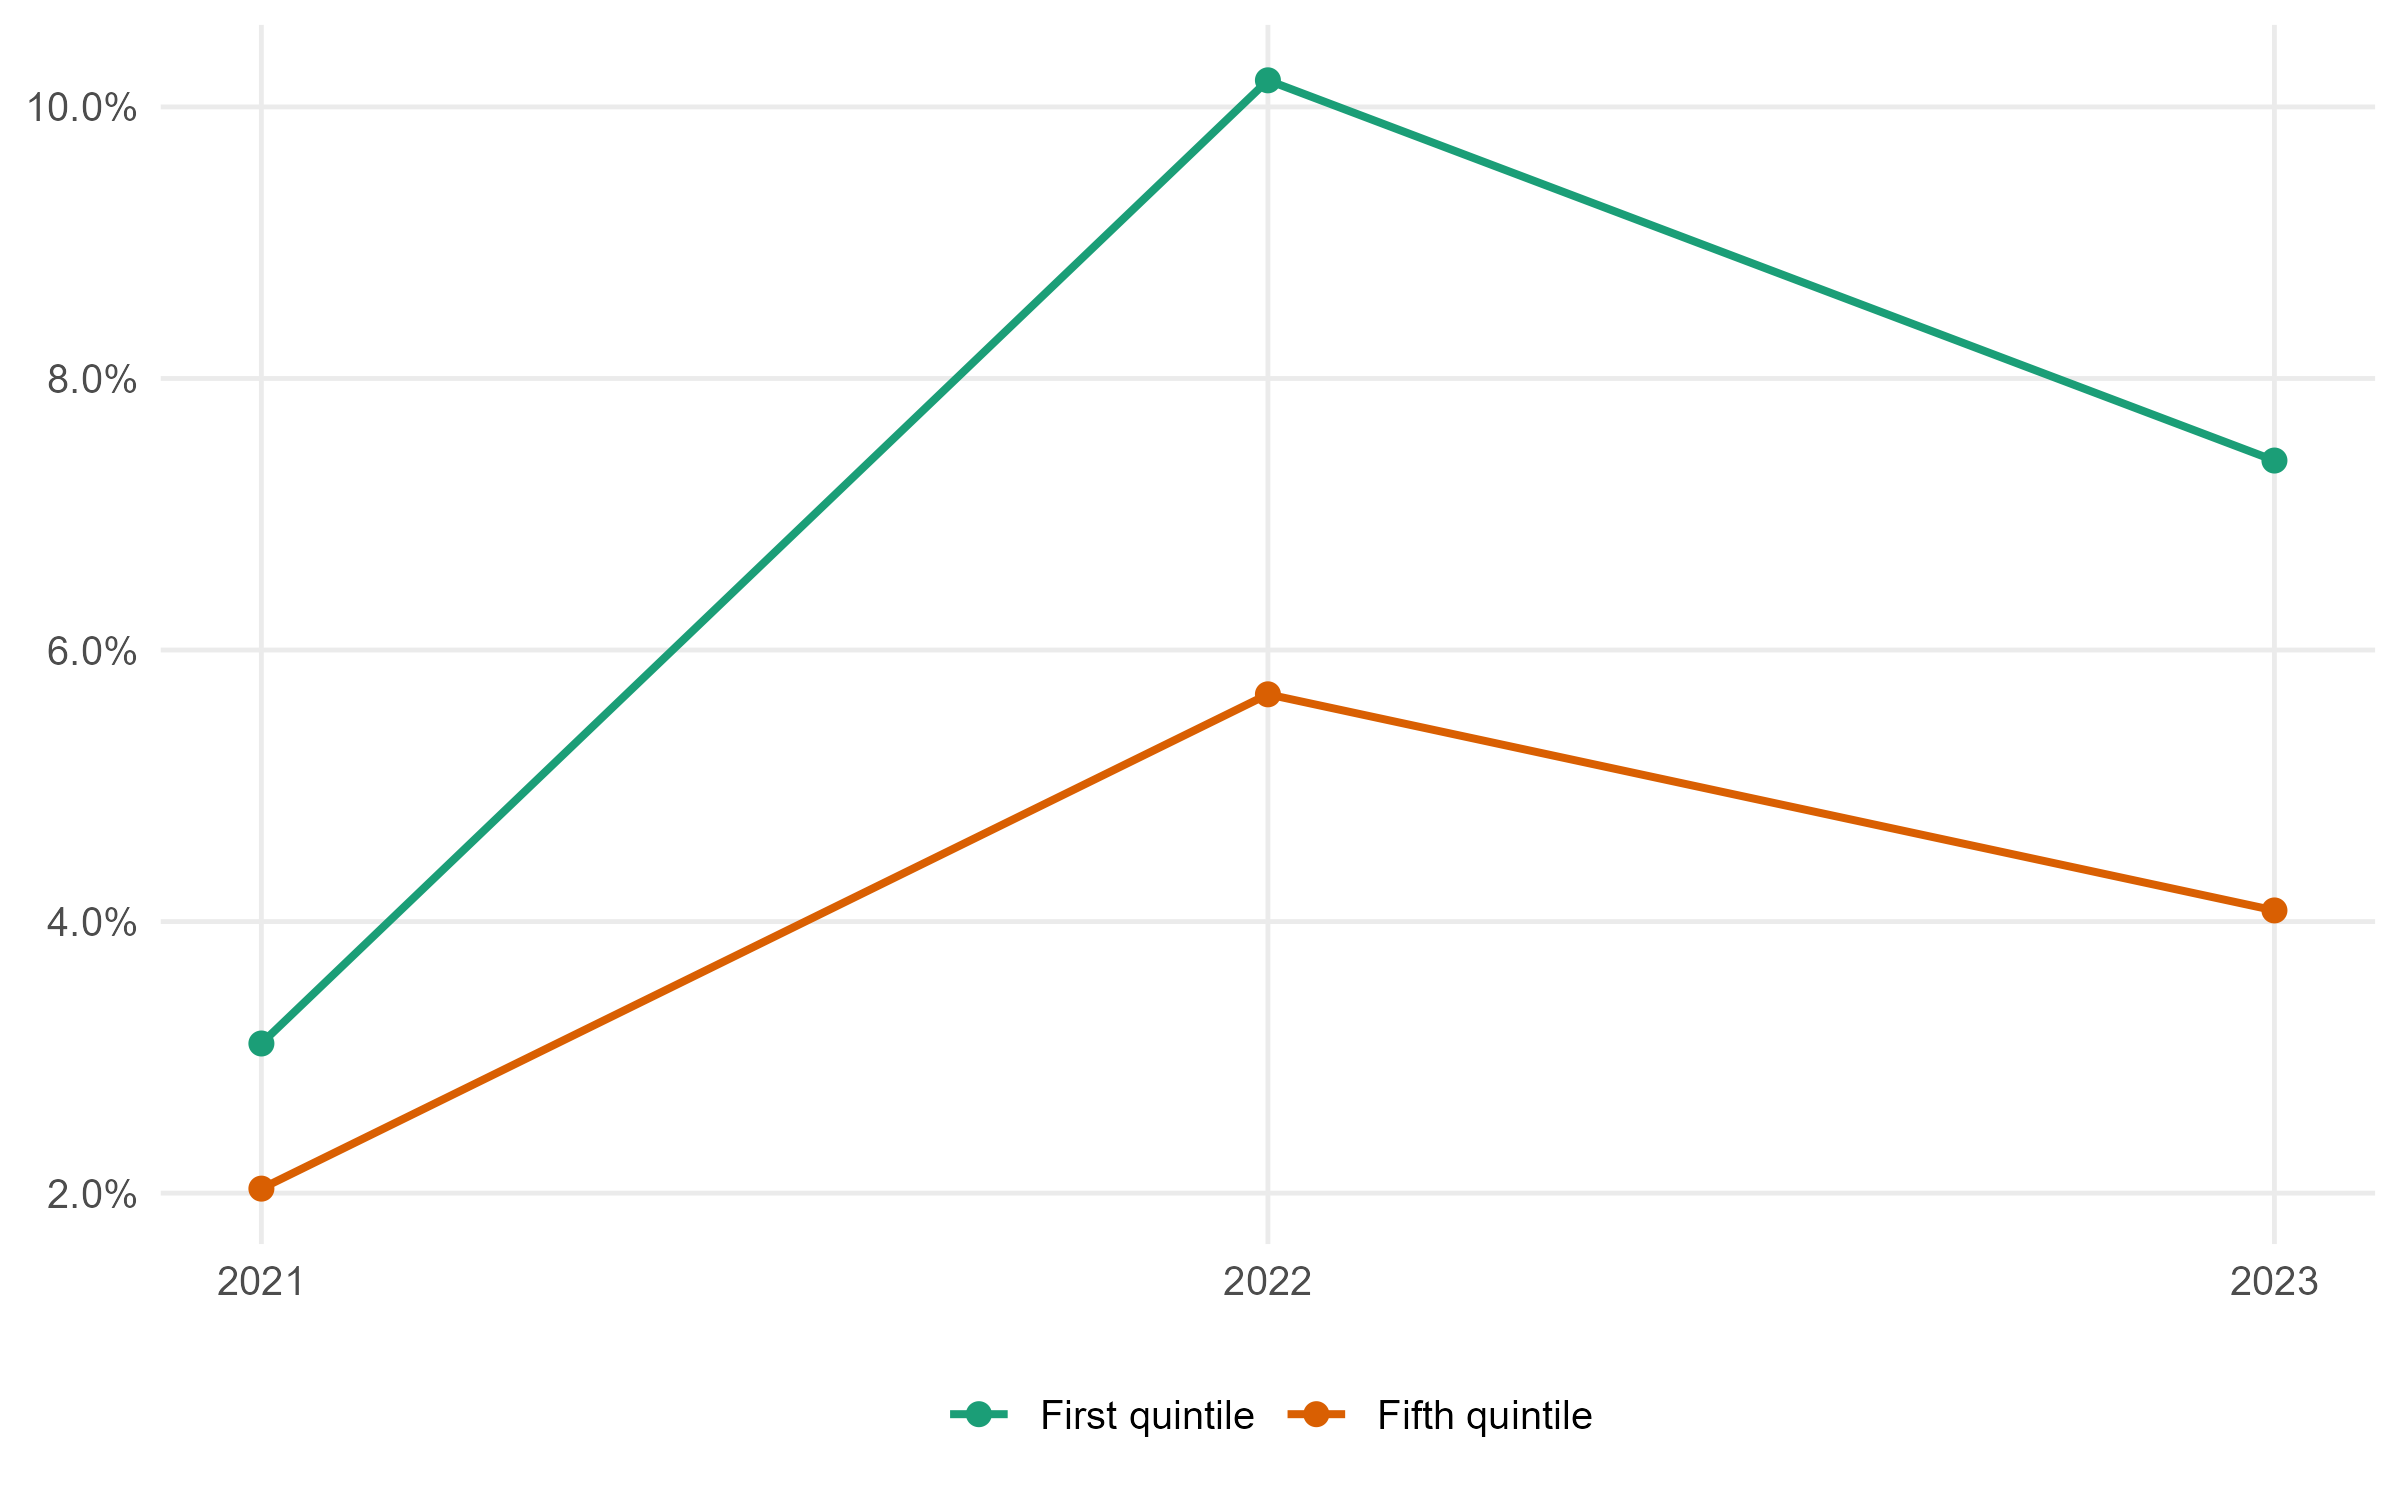
\includegraphics[width=0.86\textwidth]{fig/fig_EA20_2019_2026_income_inflation_burden_Q1_Q5.png}
\vspace{8pt}
\captionsetup{font=footnotesize, format=hang, singlelinecheck=false, justification=justified}
\caption*{Sources: Eurostat HICP, EU-SILC, HBS, authors' calculations.}
\end{figure}
%%%%%%%%%%%%%%%%%%%%%%%%%%%%%%%%%%%%%%%%%%%%%%%%%%%%%%%%%%%%%%



\newpage






\section{Effects of Unconventional Fiscal Policies on Inflation Inequality}
\label{sec:fiscal-policies}

This section evaluates the distributional effects of unconventional fiscal
policies on inflation inequality, with a particular focus on targeted
interventions such as energy price shields, VAT reductions, and fuel rebates in
the euro area.


In response to the energy crisis, euro area governments introduced a broad array of measures to cushion households from surging energy costs \citep{sgaravatti2021national,arregui2022targeted}. These included both direct income support, such as cash transfers to vulnerable groups, and price-based interventions, including temporary VAT reductions and price ceilings on gas, electricity, and fuel. While the latter are not explicitly targeted at lower-income households, they can still reduce inflation inequality by moderating the price increases of essential energy products. Cross-country evidence is consistent with this mechanism: countries with larger price-based support measures tended to display lower income-based inflation gaps during the energy crisis, whereas inflation inequality was more pronounced in countries where such measures were less extensive \citep{claeys2022inflation}.

The main measures differed substantially across euro area countries. Some governments relied primarily on regulated retail-price caps or tariff shields, while others used VAT and excise-tax reductions, fuel rebates, system-charge reductions, or calibrated block-tariff schemes. Table~\ref{tab:ea20-price-counterfactual-measures} in the appendix reports the euro-area inventory and indicates which measures are directly simulated in our price counterfactuals. We construct counterfactual price indices for the countries and policy instruments for which the necessary statutory, price, and unit-conversion information is available; Appendix~\ref{sec:app-counterfactuals} reports the corresponding country-level counterfactual series.

To quantify the effect of these fiscal measures on inflation inequality, we construct a counterfactual scenario in which no such price-based policies were enacted. Specifically, we compare the actual trajectory of policy-inclusive retail prices with estimated no-policy price paths for the affected products. This comparison allows us to isolate the extent to which fiscal policy contributed to reducing inflationary pressures and their unequal distribution across households. These measures are temporary support instruments rather than substitutes for monetary policy: their direct effect operates through administered prices, tax-inclusive prices, retail price ceilings, or unit rebates, and is therefore concentrated in the product categories to which they apply.

\subsection{Counterfactuals}

We distinguish three cases. First, for regulated-price shields, price caps, and administered tariffs, we recover a no-policy path from the relevant reference tariff, wholesale-price benchmark, or calibrated aggregate-equivalent policy layer. Second, for VAT and excise changes, we back out the reduced tax-inclusive price and reapply the normal rate. Third, for unit subsidies and fuel rebates, we add the statutory support amount back to reconstructed retail unit prices. Evidence from \citet{drolsbach2023pass} suggests that temporary fuel-tax reductions and discounts were largely passed through to consumer prices in 2022 in several euro area countries, although pass-through varied over time and by fuel type. This supports treating these measures as retail-price wedges in the counterfactual construction.

Counterfactual price indices are constructed at the COICOP component level by replacing the observed policy-inclusive HICP component-index path with a no-policy component-index path. Let $P_{j,t}$ denote the observed HICP component index for product $j$ in month $t$, and let $\widetilde P_{j,t}$ denote the corresponding counterfactual index. For each simulated measure, we recover a counterfactual retail price $\widetilde p_{j,t}$ and apply the implied price ratio to the observed component index:
\begin{equation}
\widetilde P_{j,t}
=
P_{j,t}
\frac{\widetilde p_{j,t}}{p_{j,t}} .
\end{equation}

\paragraph{VAT and excise-tax reductions.}
For VAT or excise-tax reductions, the observed retail price includes the reduced policy tax rate. The no-policy price is obtained by backing out the reduced tax-inclusive price and reapplying the normal tax rate:
\begin{equation}
\widetilde p_{j,t}
=
p_{j,t}
\frac{1+\tau^{0}_{j,t}}{1+\tau^{1}_{j,t}},
\end{equation}
where $\tau^{1}_{j,t}$ is the policy tax rate and $\tau^{0}_{j,t}$ is the no-policy tax rate.

\paragraph{Administered prices.}
For regulated or administered-price measures, such as electricity or gas tariff shields and retail price caps, the counterfactual price is taken from a no-policy reference path:
\begin{equation}
\widetilde p_{j,t}
=
p^{\mathrm{ref}}_{j,t}.
\end{equation}
When the observed tariff and the no-policy reference tariff are both available, the no-policy retail price is obtained by rescaling the observed price. If $T^{\mathrm{obs}}_{j,t}$ denotes the regulated tariff actually applied and $T^{\mathrm{ref}}_{j,t}$ the tariff that would have applied without the intervention, then:
\begin{equation}
p^{\mathrm{ref}}_{j,t}
=
p_{j,t}
\frac{T^{\mathrm{ref}}_{j,t}}{T^{\mathrm{obs}}_{j,t}} .
\end{equation}
When the policy is defined through a wholesale-price intervention rather than an explicit retail tariff schedule, the no-policy retail-price benchmark is estimated from the pre-intervention relationship between retail prices and wholesale market prices. Let $WPE_t$ denote the wholesale electricity price and let $D_t$ collect seasonal controls. The benchmark is obtained from
\begin{equation}
\log p^{\mathrm{ref}}_{j,t}
=
\widehat\alpha
+
\widehat\beta \log WPE^{\mathrm{ref}}_t
+
D_t'\widehat\gamma ,
\end{equation}
where the coefficients are estimated before the intervention period and $WPE^{\mathrm{ref}}_t$ is the wholesale price benchmark. The data sources used for each country-specific reference path are documented in the policy inventory and appendix.

\paragraph{Subsidies and rebates.}
For unit subsidies, fuel rebates, or per-kWh support schemes, the observed price is lower than the no-policy price by the statutory support amount. The counterfactual price is obtained by adding the support amount $s_{j,t}$ back to the observed unit price:
\begin{equation}
\widetilde p_{j,t}
=
p_{j,t}+s_{j,t}.
\end{equation}
For transport-fuel rebates, $s_{j,t}$ is recovered from the statutory pump discount, expressed in euros per litre, and applied to a monthly retail-fuel price consistent with the HICP transport-fuel component. Following \citet{bonnet2025compensating}, we refer to these interventions as pump-price rebates or subsidies because they reduced the tax-inclusive price paid by consumers, although their technical implementation sometimes operated through fuel excise taxation rather than through a direct transfer to households. The no-rebate fuel index is obtained by rescaling the observed HICP transport-fuel component:
\[
\widetilde P_{j,t}
=
P_{j,t}
\frac{p^{M}_{j,t}+s_{j,t}}{p^{M}_{j,t}} .
\]
Outside the months in which a rebate is active, the observed and counterfactual fuel indices coincide. When only part of the statutory rebate was borne by the public sector or passed through to the posted retail price, the effective amount added back to the observed price is adjusted accordingly, using the country-specific information reported in the policy inventory.

For a small set of price-relevant interventions, the policy inventories identify the measure but do not provide the monthly no-policy tariff schedule, tariff-block utilization, or eligible-household weights needed for a direct statutory reconstruction. We therefore add these cases as separate calibrated layers, identified from \citet{sgaravatti2021national} and \citet{arregui2022targeted}, rather than merging them with the VAT or unit-subsidy calculations. This applies to block-tariff or price-cap schemes in Germany, the Netherlands, Cyprus, Ireland, Italy, and Slovenia, and to Belgium's extension of the social energy tariff and basic energy package. The calibrated ratios are applied only to the relevant COICOP energy components and policy months, and the corresponding assumption tables are reported with the counterfactual outputs. These layers should be interpreted as aggregate-equivalent price effects, not as micro-founded statutory tariff reconstructions.

The counterfactual component indices are then used in the same household-group
inflation procedure as the observed indices. Replacing the observed component
indices $P_{j,t}$ with $\widetilde P_{j,t}$ yields a chained counterfactual
group index $\widetilde I_{g,t}$. The counterfactual inflation rate for group
$g$ is then computed as the year-on-year growth rate of this index, as in the
package implementation:
\begin{equation}
\widetilde \pi_{g,t}
=
100\left(
\frac{\widetilde I_{g,t}}{\widetilde I_{g,t-12}}-1
\right).
\end{equation}



\subsection{Euro Area}

We aggregate the country-level policy counterfactuals to the euro-area level using Eurostat country weights for the HICP. The aggregation is performed over the set of countries for which a price-policy counterfactual is simulated, with country weights renormalized within this policy sample in each year. This produces a common-scope comparison between the observed country-weighted policy-sample index and the corresponding no-policy counterfactual. We also report the official euro-area HICP index as an external benchmark for the observed aggregate series.

Figure~\ref{fig:ea_policy_total_cpi_counterfactual} shows that the simulated fiscal measures compressed euro-area inflation during the energy crisis. The gap between the observed policy-sample index and the counterfactual index is largest around the peak of the 2022--23 energy shock, when VAT reductions, fuel rebates, price shields, regulated-price caps, and calibrated block-tariff layers were simultaneously active across countries. The official euro-area HICP remains close to the observed policy-sample aggregate, while not coinciding exactly because the policy sample excludes countries without a simulated price-policy layer and because the aggregation is restricted to the countries covered by the counterfactual exercise.

\begin{figure}[H]
\centering
\caption{Euro area: country-weighted policy counterfactual and official HICP inflation (in \%)}
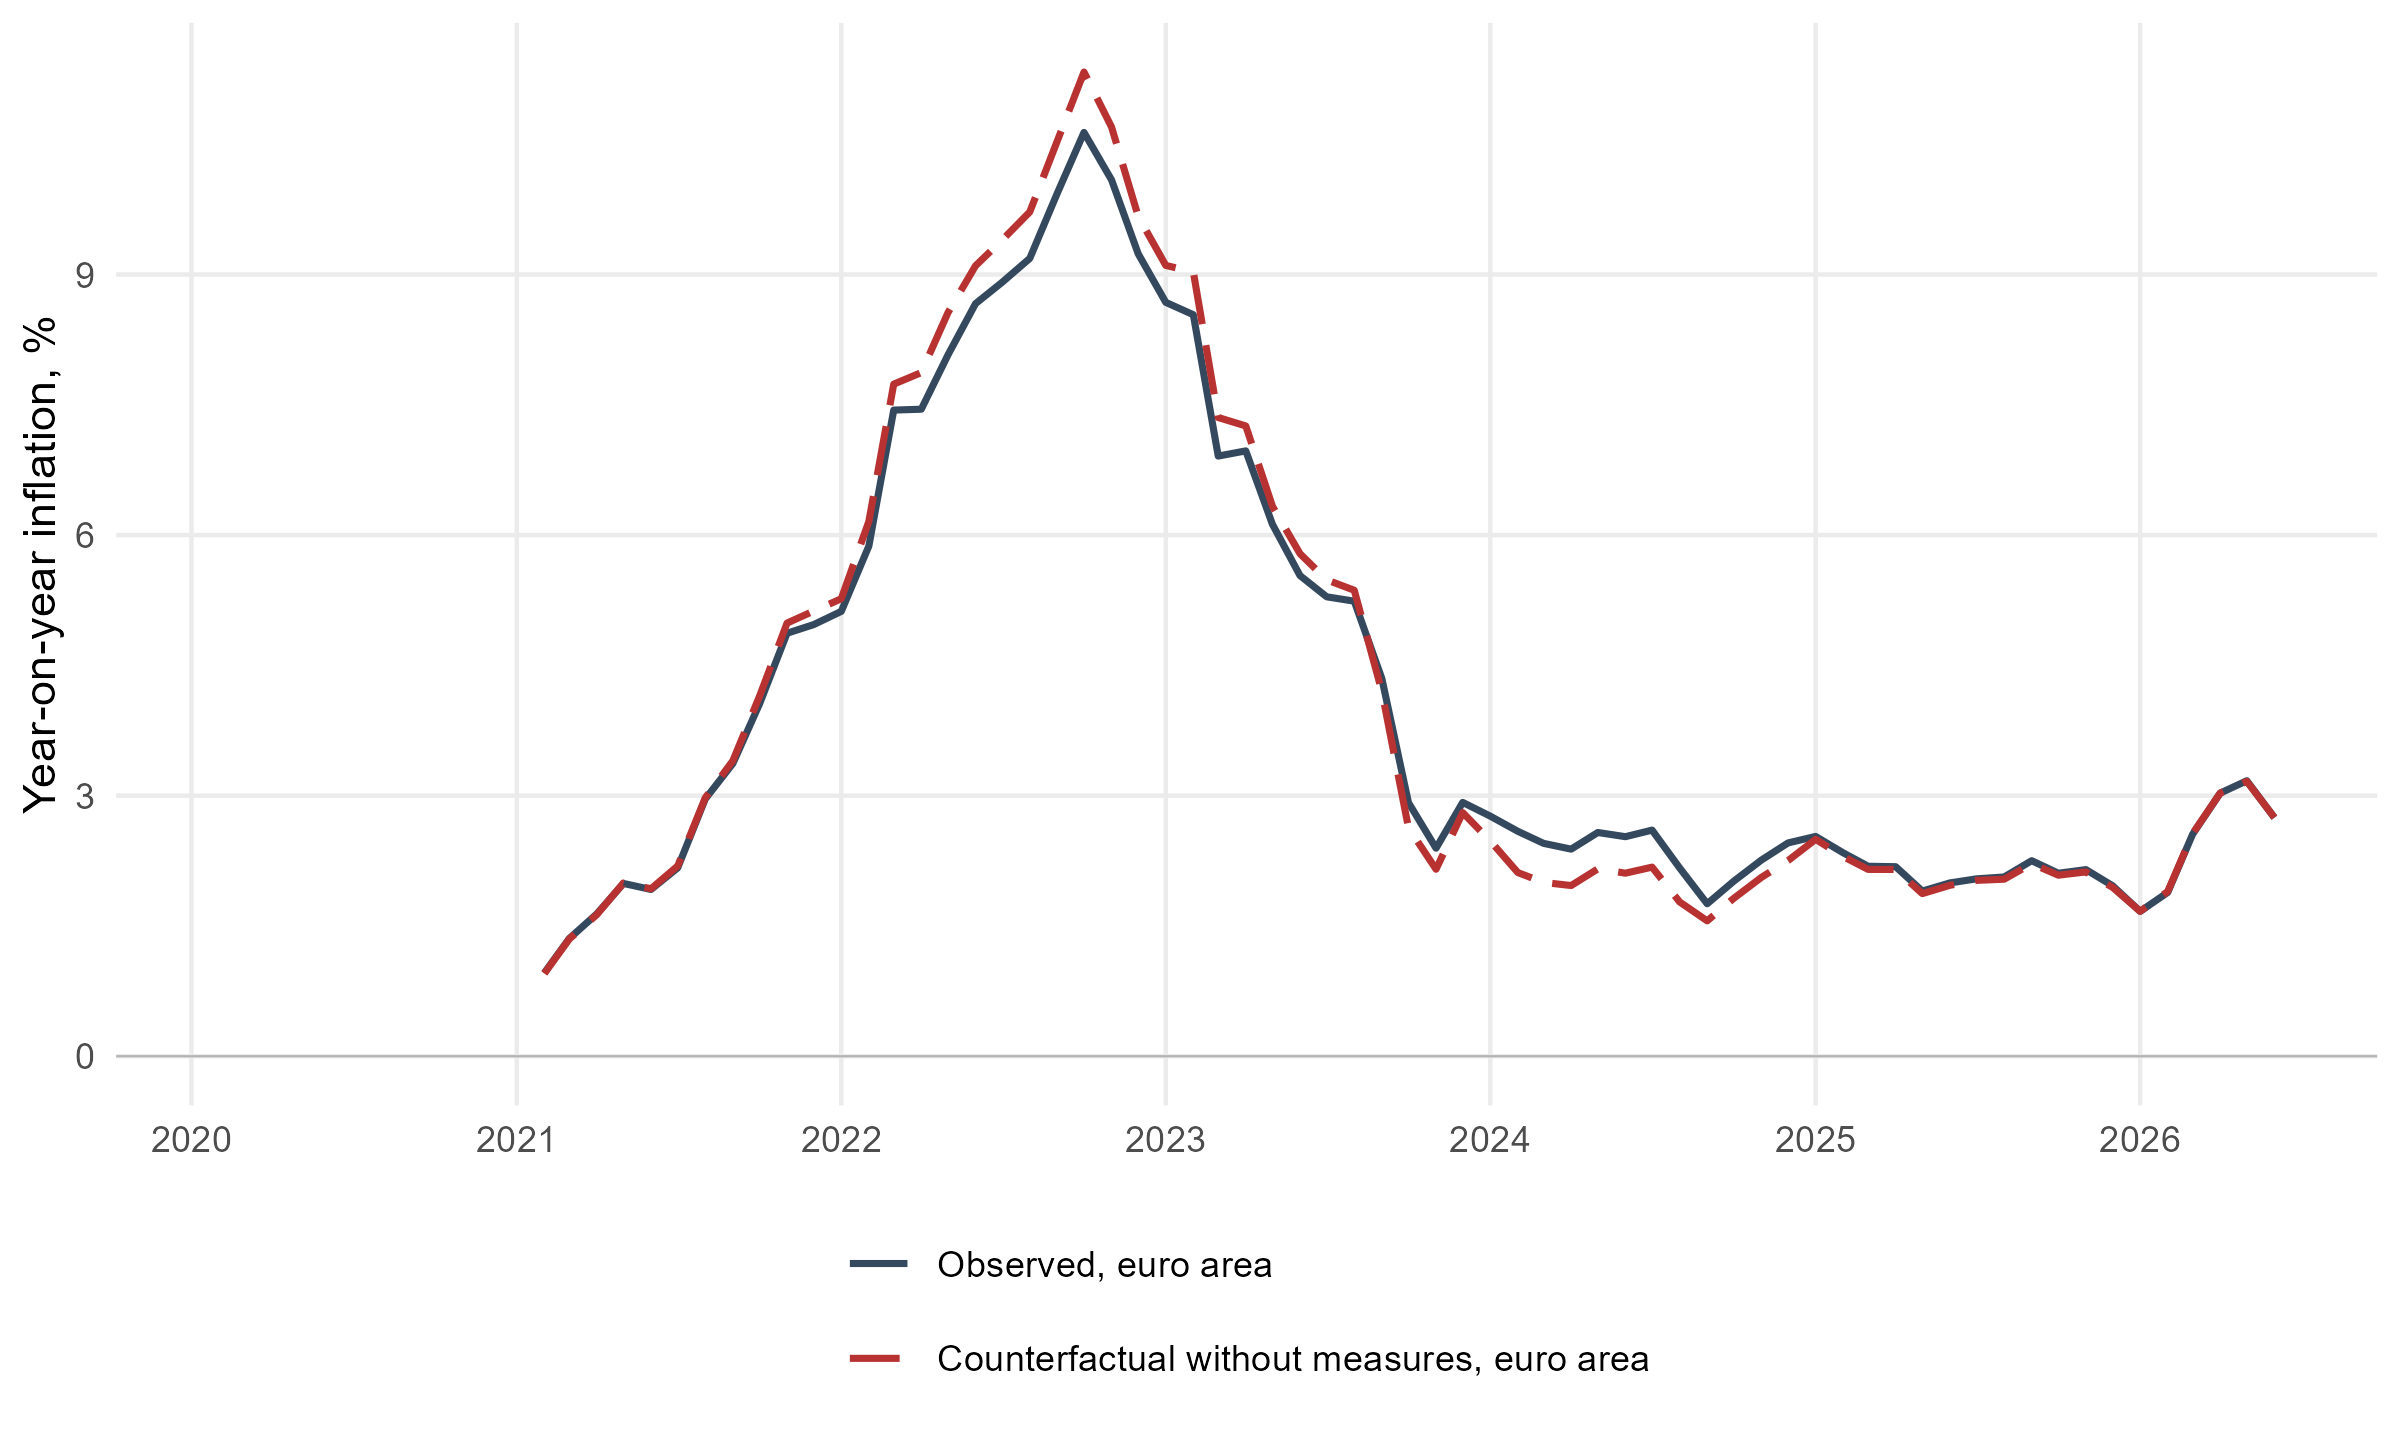
\includegraphics[width=0.86\textwidth,height=0.42\textheight,keepaspectratio]{fig/policy_total_cpi_counterfactual_inflation_EA_policy_sample.png}
\label{fig:ea_policy_total_cpi_counterfactual}
\captionsetup{font=footnotesize, format=hang, singlelinecheck=false, justification=justified}
\caption*{Notes: The figure compares three year-on-year inflation series: observed headline HICP inflation aggregated from the countries covered by the policy counterfactual exercise, the corresponding counterfactual inflation rate without the simulated price-policy measures, and official euro-area HICP inflation. Country aggregation uses Eurostat euro-area country weights, renormalized within the policy sample in each year. Unit: year-on-year inflation rate, in percent.\\
Source: Eurostat HICP and country weights, Bruegel energy-policy dataset, IMF policy inventory, national policy sources, authors' calculations.}
\end{figure}

%%%%%%%%%%%%%%%%%%%%%%%%%%%%%%%%%%%%%%%%%%%%%%%%%%%%%%%%%%%%%%

%Fiscal policy can best contribute to mitigating the negative impact of inflation on households through targeted and temporary support measures (tariff protection, increases in pensions and social benefits).

% These measures must be temporary; fiscal policy is not intended to combat inflation, particularly in indebted countries. Monetary and fiscal policies each have a role to play in addressing the consequences of high inflation. In the long run, only monetary policy is effective in bringing inflation back to its target.


\section{Household-level inflation}
\label{sec:household-level}

Group-level inflation is useful for comparability across countries, but it only captures the component of inflation inequality that arises between broad household categories, such as income quintiles, age groups, or residence areas. These categories remain internally heterogeneous: two households in the same income quintile, age group, or rural area may differ in housing tenure, family composition, heating technology, car use, and detailed consumption patterns. A substantial part of inflation dispersion may therefore persist within the categories used in the previous sections. Measuring inflation at the household level is useful for documenting this residual dispersion and for separating the respective roles of household characteristics that are correlated in grouped comparisons. To document this within-group heterogeneity, we use household-level HBS expenditure data and compute household-specific inflation rates. In the empirical application, we use the Spanish EPF, a publicly available HBS microdata source, and match each annual price index to the preceding EPF wave. The HBS survey year is denoted $y'=y-1$ in the expenditure-share formulas below. For each household, expenditure shares are matched to monthly COICOP price indices from the HICP. Household-level inflation is then obtained from the household-specific price index implied by the household's own expenditure shares. The distributions below are weighted using the EPF survey weights.

\subsection{Calculating household inflation rates with consumer price indices}

We apply one-year-lagged fixed-basket Laspeyres logic at the household level.
Let $e^{HBS}_{i,j,y'}$ denote household $i$'s expenditure on COICOP item $j$ in
HBS wave $y'$, and let $a_{i,y'}$ denote its survey weight. The household
expenditure share is
\begin{equation}
\omega^{HBS}_{j,i,y'}
=
\frac{a_{i,y'}e^{HBS}_{i,j,y'}}{\sum_{k \in \mathcal{J}_{i,y'}} a_{i,y'}e^{HBS}_{i,k,y'}}
=
\frac{e^{HBS}_{i,j,y'}}{\sum_{k \in \mathcal{J}_{i,y'}} e^{HBS}_{i,k,y'}}
\end{equation}
using the same convention as the group-specific weights $\omega_{j,g,y}$
defined above. Since the same survey weight applies to all items within a
household, it cancels out in the within-household basket; it is then used to
weight households when constructing cross-household distributions and summary
statistics. For household $i$,
the within-year price index in month $m$ of year $y$ is
\begin{equation}
P_{i,y,m}
=
\sum_{j \in \mathcal{J}_{i,y',y}}
\omega^{HBS}_{j,i,y'}
\frac{p_{j,y,m}}{p_{j,y,0}}
,
\end{equation}
where $\mathcal{J}_{i,y',y}$ is the set of household expenditure items observed
in HBS wave $y'$ that can be matched to HICP prices in year $y$. Households are
therefore treated as elementary household groups: the within-year Laspeyres
movements are chain-linked at the household level, and year-on-year monthly
inflation rates $\pi_{i,y,m}$ are computed from the resulting chained household
price index.

%This formula loops over households, product categories, and months. It is more
%computationally demanding than the faster approximation that first aggregates
%item-level annual inflation and then applies household expenditure shares, but
%it is closer to the index construction used for the group-level indicators.

Figure~\ref{fig:es-household-level-distribution} overlays the cross-household distributions for 2021, 2022, and 2023 using bins of 0.1 percentage point. Weighted mean household inflation is about 3.1 percent in 2021, 7.2 percent in 2022, and 2.7 percent in 2023. The distribution shifts markedly to the right in 2022 and becomes more dispersed, with a visible upper tail around and above 10 percent. This pattern is consistent with the broad-based energy and food price shock observed in Spain during that year. In 2021 and 2023, household-level inflation is lower and the mass of the distribution is closer to the 2--4 percent range, although both years retain non-negligible heterogeneity across households.

%%%%%%%%%%%%%%%%%%%%%%%%%%%%%%%%%%%%%%%%%%%%%%%%%%%%%%%%%%%%%%
\begin{figure}[H]
\centering
\caption{Distribution of household-level inflation in Spain (in \%)}
\label{fig:es-household-level-distribution}
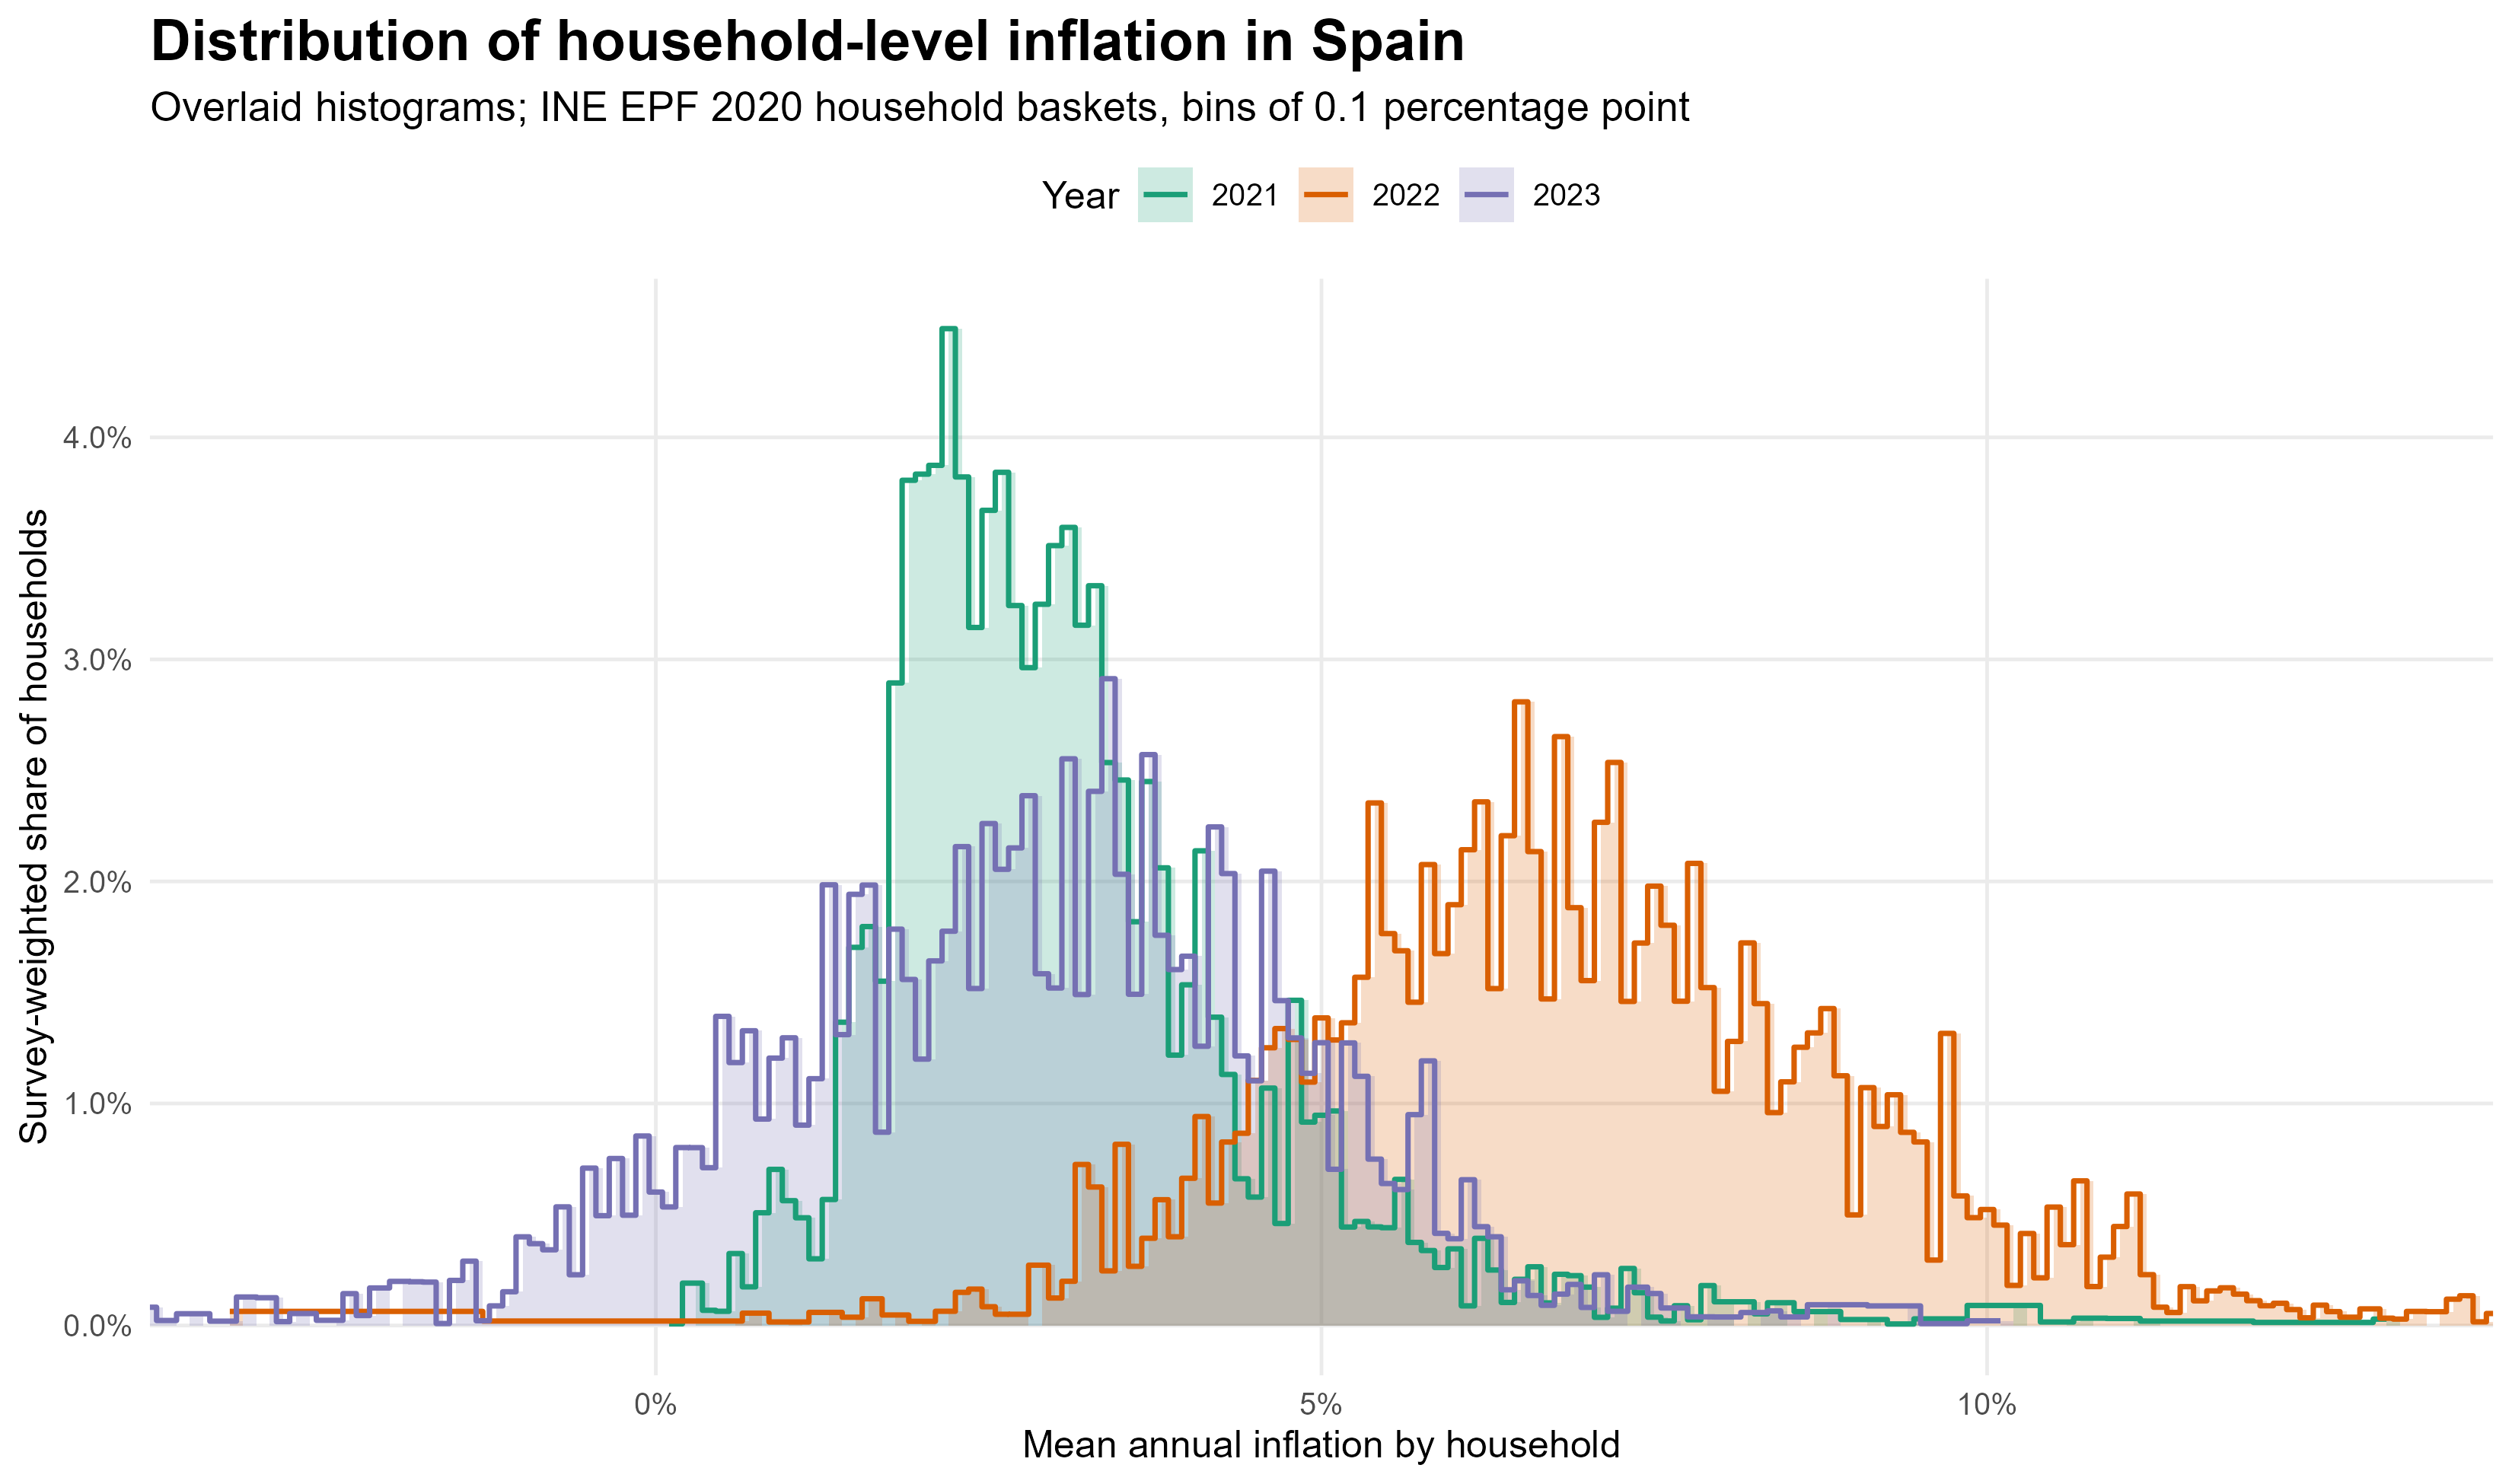
\includegraphics[width=0.9\textwidth]{fig/fig_ES_household_level_inflation_distribution.png}
\vspace{8pt}
\captionsetup{font=footnotesize, format=hang, singlelinecheck=false, justification=justified}
\caption*{Notes: The figure reports the survey-weighted cross-household distribution of mean annual household inflation rates. The horizontal axis reports household-level mean annual inflation rates, in percent; the vertical axis reports the survey-weighted share of households, in percent. Household baskets are taken from the preceding EPF wave: 2020 for 2021 inflation, 2021 for 2022 inflation, and 2022 for 2023 inflation.\\
Sources: INE EPF 2020--2022 microdata, Eurostat HICP, authors' calculations.}
\end{figure}
%%%%%%%%%%%%%%%%%%%%%%%%%%%%%%%%%%%%%%%%%%%%%%%%%%%%%%%%%%%%%%


Figure~\ref{fig:es-household-level-distribution-q1-q5} compares the 2023 distributions for households in the first and fifth quintiles of equivalised income. The two distributions overlap substantially, while the fifth quintile has a higher weighted mean and a slightly higher median in 2023. The result indicates that, after the 2022 peak, household-level inflation heterogeneity remains visible within the income distribution, but the difference between the bottom and top quintiles is modest relative to the dispersion within each group.


%%%%%%%%%%%%%%%%%%%%%%%%%%%%%%%%%%%%%%%%%%%%%%%%%%%%%%%%%%%%%%
\begin{figure}[H]
\centering
\caption{Household-level inflation in Spain by income quintile, 2023 (in \%)}
\label{fig:es-household-level-distribution-q1-q5}
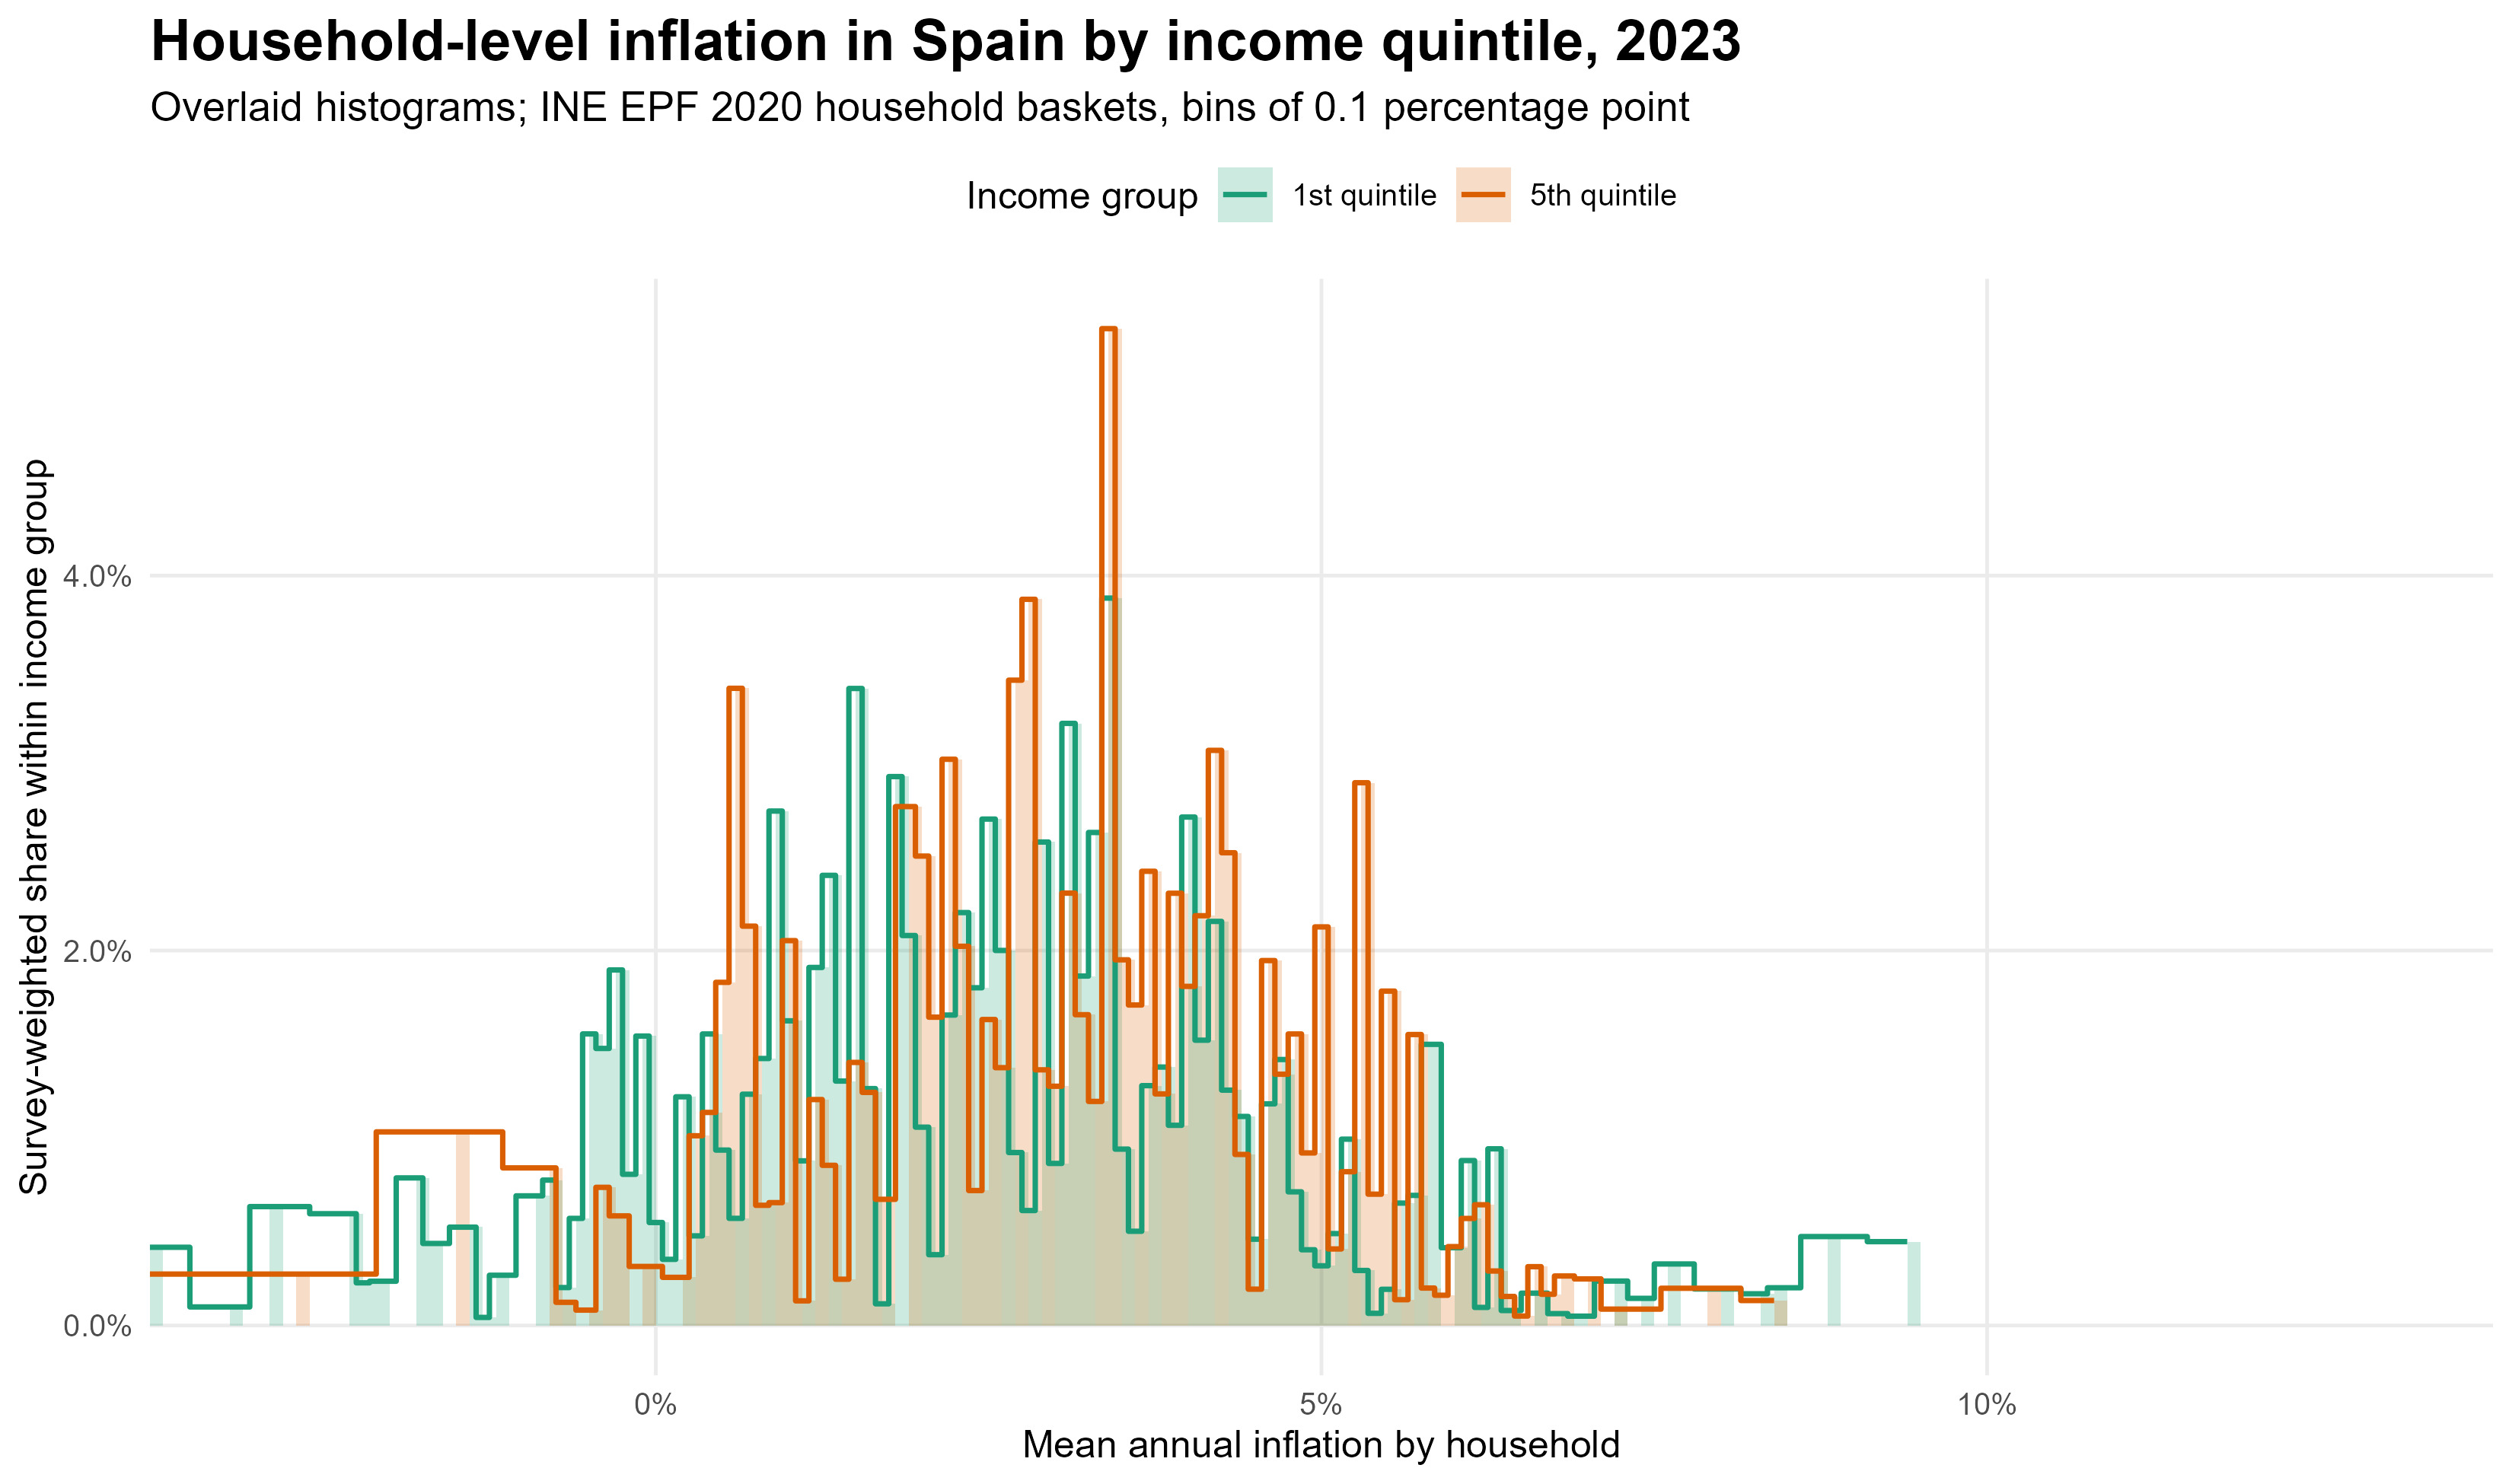
\includegraphics[width=0.9\textwidth]{fig/fig_ES_household_level_inflation_distribution_q1_q5_2023.png}
\vspace{8pt}
\captionsetup{font=footnotesize, format=hang, singlelinecheck=false, justification=justified}
\caption*{Notes: The figure reports the survey-weighted cross-household distribution of mean annual household inflation rates in 2023 for the first and fifth quintiles of equivalised income. The horizontal axis reports household-level mean annual inflation rates, in percent; the vertical axis reports the survey-weighted share of households within each income quintile, in percent. Household baskets and quintiles are computed from the 2022 EPF wave using EPF survey weights.\\
Sources: INE EPF 2022 microdata, Eurostat HICP, authors' calculations.}
\end{figure}
%%%%%%%%%%%%%%%%%%%%%%%%%%%%%%%%%%%%%%%%%%%%%%%%%%%%%%%%%%%%%%
\newpage
\subsection{Analysis of Variance}

Table~\ref{tab:es-epf-inflation-regressions-by-year} reports year-by-year
regressions of household-level annual inflation on observed household
characteristics in the Spanish EPF. Table~\ref{tab:es-epf-inflation-regressions-pooled}
reports the corresponding pooled specifications, with and without year fixed
effects. These regressions ask how much of the dispersion visible in the
household-level distributions can be associated with each characteristic,
holding the other observed household characteristics constant.

\begin{table}[H]
\centering
\caption{Household-level inflation regressions by year, Spain}
\label{tab:es-epf-inflation-regressions-by-year}
\scriptsize
\setlength{\tabcolsep}{3pt}
\renewcommand{\arraystretch}{0.9}

\begingroup
\centering
\begin{tabular}{lccc}
   \tabularnewline \midrule \midrule
   Dependent Variable: & \multicolumn{3}{c}{Annual household inflation}\\
   Year                & 2021            & 2022            & 2023 \\   
   Model:              & (1)             & (2)             & (3)\\  
   \midrule
   \emph{Variables}\\
   Constant            & 4.088$^{***}$   & 8.376$^{***}$   & 1.873$^{***}$\\   
                       & (0.1397)        & (0.2492)        & (0.3011)\\   
   Less than 30 years  & -0.1147         & -0.4044         & 0.2111\\   
                       & (0.1920)        & (0.3039)        & (0.2872)\\   
   From 30 to 44 years & -0.0328         & -0.1749         & 0.1131\\   
                       & (0.0890)        & (0.1576)        & (0.1876)\\   
   From 45 to 59 years & -0.0954         & -0.1185         & 0.0921\\   
                       & (0.0962)        & (0.1560)        & (0.1939)\\   
   Income quintile 2   & -0.0580         & -0.0305         & 0.3459\\   
                       & (0.1103)        & (0.2095)        & (0.2409)\\   
   Income quintile 3   & -0.2967$^{**}$  & -0.3132$^{*}$   & 0.0889\\   
                       & (0.1214)        & (0.1861)        & (0.2434)\\   
   Income quintile 4   & -0.3234$^{***}$ & -0.4341$^{**}$  & 0.1323\\   
                       & (0.1007)        & (0.2081)        & (0.2504)\\   
   Income quintile 5   & -0.5108$^{***}$ & -0.7099$^{***}$ & 0.3368\\   
                       & (0.1128)        & (0.2128)        & (0.2388)\\   
   Owner               & 0.0573          & 1.358$^{***}$   & 2.133$^{***}$\\   
                       & (0.1028)        & (0.1424)        & (0.1284)\\   
   Towns and suburbs   & -0.6069$^{***}$ & -0.5777$^{***}$ & 0.4842$^{**}$\\   
                       & (0.1214)        & (0.2103)        & (0.2311)\\   
   Cities              & -0.9354$^{***}$ & -1.338$^{***}$  & 0.2149\\   
                       & (0.1119)        & (0.2054)        & (0.2286)\\   
   \midrule
   \emph{Fit statistics}\\
   Observations        & 2,283           & 2,098           & 2,570\\  
   R$^2$               & 0.09960         & 0.13365         & 0.07975\\  
   \midrule \midrule
   \multicolumn{4}{l}{\emph{Heteroskedasticity-robust standard-errors in parentheses}}\\
   \multicolumn{4}{l}{\emph{Signif. Codes: ***: 0.01, **: 0.05, *: 0.1}}\\
\end{tabular}
\par\endgroup



\vspace{4pt}
\captionsetup{font=footnotesize, format=hang, singlelinecheck=false, justification=justified}
\caption*{Notes: The dependent variable is household-level mean annual inflation, in percent. Regressions are estimated separately by inflation year using EPF survey weights. The omitted categories are households whose reference person is aged 60 years or over, income quintile 1, renters or other tenure statuses, and rural areas.\\
Sources: INE EPF 2020--2022 microdata, Eurostat HICP, authors' calculations.}
\end{table}

\begin{table}[H]
\centering
\caption{Pooled household-level inflation regressions, Spain}
\label{tab:es-epf-inflation-regressions-pooled}
\scriptsize
\setlength{\tabcolsep}{3pt}
\renewcommand{\arraystretch}{0.9}

\begingroup
\centering
\begin{tabular}{lcc}
   \tabularnewline \midrule \midrule
   Dependent Variable: & \multicolumn{2}{c}{Annual household inflation}\\
   Specification       & Pooled          & Year FE \\   
   Model:              & (1)             & (2)\\  
   \midrule
   \emph{Variables}\\
   Constant            & 5.070$^{***}$   &   \\   
                       & (0.1786)        &   \\   
   Less than 30 years  & -0.3517$^{*}$   & -0.1042\\   
                       & (0.2017)        & (0.1509)\\   
   From 30 to 44 years & -0.1809         & -0.0217\\   
                       & (0.1192)        & (0.0878)\\   
   From 45 to 59 years & -0.2196$^{*}$   & -0.0551\\   
                       & (0.1245)        & (0.0907)\\   
   Income quintile 2   & 0.0519          & 0.0713\\   
                       & (0.1473)        & (0.1120)\\   
   Income quintile 3   & -0.1353         & -0.1510\\   
                       & (0.1474)        & (0.1092)\\   
   Income quintile 4   & -0.2246         & -0.2139$^{*}$\\   
                       & (0.1486)        & (0.1117)\\   
   Income quintile 5   & -0.2708$^{*}$   & -0.2707$^{**}$\\   
                       & (0.1496)        & (0.1119)\\   
   Owner               & 1.171$^{***}$   & 1.188$^{***}$\\   
                       & (0.1144)        & (0.0758)\\   
   Towns and suburbs   & -0.6261$^{***}$ & -0.3266$^{***}$\\   
                       & (0.1456)        & (0.1067)\\   
   Cities              & -0.9399$^{***}$ & -0.7847$^{***}$\\   
                       & (0.1374)        & (0.1024)\\   
   \midrule
   \emph{Fixed-effects}\\
   year                &                 & Yes\\  
   \midrule
   \emph{Fit statistics}\\
   Observations        & 6,951           & 6,951\\  
   R$^2$               & 0.04003         & 0.49186\\  
   Within R$^2$        &                 & 0.06669\\  
   \midrule \midrule
   \multicolumn{3}{l}{\emph{Heteroskedasticity-robust standard-errors in parentheses}}\\
   \multicolumn{3}{l}{\emph{Signif. Codes: ***: 0.01, **: 0.05, *: 0.1}}\\
\end{tabular}
\par\endgroup



\vspace{4pt}
\captionsetup{font=footnotesize, format=hang, singlelinecheck=false, justification=justified}
\caption*{Notes: The dependent variable is household-level mean annual inflation, in percent. Both specifications use EPF survey weights. The second specification includes inflation-year fixed effects. The omitted categories are households whose reference person is aged 60 years or over, income quintile 1, renters or other tenure statuses, and rural areas.\\
Sources: INE EPF 2020--2022 microdata, Eurostat HICP, authors' calculations.}
\end{table}

The specification with year fixed effects indicates that age differences
are limited once common year effects are controlled for. The income-group breakdown is
also modest, although households in the top quintile experience inflation about
0.27 percentage point lower than households in the first quintile. By contrast,
housing tenure and residence density remain strongly associated with
household-level inflation: owners record higher inflation, while households in
cities record lower inflation than those in rural areas. 



\section{Conclusion}


%This paper a set of public indicators to measure inflation inequalities in real-time monthly across socio-demographic groups in the Euro Area.

This paper presents a methodology for building timely inflation inequality indicators in the euro area based on the Harmonised Index of Consumer Prices (HICP) and household budget surveys. It provides a framework for monitoring how aggregate inflation translates into different household-group inflation rates across countries and over time.

%results
Our results show that inflation inequality across income groups in the euro area has remained contained during the recent inflationary episode in several large countries, especially Germany, France, and Spain. We also document strong cross-country heterogeneity in inflation inequality, including more pronounced disparities in Italy and in countries dependent on natural gas imports, such as the Baltic states. 

Inflation inequalities by age and residence are more pronounced, with older and rural households generally facing higher inflation, consistent with their larger expenditure shares on essential goods such as food and energy. We also find that unconventional fiscal measures, including VAT cuts and energy price shields, mitigated inflation inequality, especially among lower-income households. These measures operated directly on relative prices, particularly energy prices, and therefore reduced both average inflation and the inflation exposure of groups whose baskets were more energy intensive.

%Consumption-based inflation inequality captures only one dimension of the distributional effects of inflation. A complete assessment also requires accounting for income indexation, transfers, and wealth effects, which may dominate consumption-basket effects for some households \citep{cardoso2022heterogeneous,pallotti2024bears}.

Fiscal packages such as VAT reductions, fuel rebates, and tariff shields can have immediate effects on measured prices and can change relative prices across consumption categories. They can reduce the inflation burden of households whose expenditure is concentrated on regulated or subsidized items. At the same time, the income-group breakdown is not sufficient to identify vulnerable households: exposure also depends on residence area, heating technology, mobility constraints, and the capacity to substitute away from energy-intensive consumption.

By contrast, monetary policy affects the aggregate price level through broader transmission channels, with lags generally estimated at around 18 months. In the long run, monetary policy remains the instrument responsible for bringing inflation back to its target, including the 2 percent objective in the euro area, while fiscal policy is better understood as a temporary instrument for cushioning distributional effects during large relative-price shocks.

%limit
The group-level indicators remain subject to aggregation bias. To improve accuracy, it is essential to compute inflation inequality indicators at the most granular level available within the consumption product classification. Recent advances in data availability, such as supermarket scanner data at the bar-code level or bank transaction records, provide new opportunities to improve the precision of inflation and consumption measurement.

%Granular data make it possible to take into account the income channels, wage indexation to inflation, as well as wealth effects. \cite{cardoso2022heterogeneous} show that in Spain, the distributional effects of inflation through household wealth and income outweigh those arising from consumption patterns. Similarly, \cite{pallotti2024bears} find that net household wealth is the primary driver of inflation inequality across six euro area countries (Germany, France, Italy, Spain, the Netherlands, and Belgium). Their findings highlight that older households are disproportionately affected, primarily due to the adverse impact of inflation on their wealth.

%policy implications
%The heterogeneous impact of inflation across household categories suggests the need for carefully calibrated policy responses. While monetary policy remains the primary tool for controlling aggregate inflation, targeted fiscal measures may be necessary to address acute distributional concerns during periods of elevated inflation.

%Understanding the heterogeneous effects of inflation is crucial to design policies that support vulnerable households face inflationary shocks. While fiscal policy can provide temporary relief, only monetary policy can bring inflation back to target in the long run.
%Monetary policy channel of transmission have lags. What role should fiscal measures in the short run, such as targeted VAT reductions, play in mitigating inflation for the most vulnerable households? 

%Possible Extensions Possible extension of this paper for the Euro Area could be first non-homothetic price indices that allows for a more accurate representation of consumption patterns across income groups (Jaravel and Lashkari 2023). S






% Bibliographie

 \bibliographystyle{ecta}
 \bibliography{references}
\nocite{*}


\clearpage 

\appendix

%%%%%%%%%%%%%%%%%%%%%%%%%%%%%%%%%%%%%%%%%   APPENDIX  -- SETTING COUNTERS TO ZERO 
\setcounter{figure}{0}
\setcounter{table}{0}

% \renewcommand{\thesubsection}{\arabic{subsection})}
%\renewcommand{\thetable}{\Roman{table}}
%\renewcommand{\thefigure}{\Roman{figure}}
\counterwithin{figure}{section}
\counterwithin{table}{section}
\renewcommand{\thefigure}{\Alph{section}.\arabic{figure}}
\renewcommand{\thetable}{\Alph{section}.\arabic{table}}

%\pagenumbering{roman}
 \setcounter{page}{1}
\begin{center}

{\textbf{\Large  Appendix     \\ }}\vspace{0.3cm}
\Large {Erwan Gautier - Jérémi Montornès} \\
\vspace{1cm}
{\Large(Not for publication)}\\
\vspace{1cm}
\today\\



\end{center}




%\addcontentsline{toc}{section}{Annexes}

%\renewcommand{\thetable}{\Alph{section}} 
%\renewcommand{\thefigure}{\Alph{section}} 

\section{Heterogeneous Effects of Shocks}
\label{sec:app-heterogeneous-shocks}

\section*{Input-output price shocks and inflation inequality}
\begin{table}[H]
\centering
\caption{Cumulative Energy Shock Exposure, June 2021--June 2023}
\scriptsize
\setlength{\tabcolsep}{1.2pt}
\begin{tabular}{lrrrrrrr}
\toprule
Country & \shortstack{Effect on average\\inflation -- Total} & \shortstack{Direct effect on\\average inflation} & \shortstack{Indirect effect on\\average inflation} & \shortstack{Indirect effect on average\\inflation through trade} & \shortstack{Effect on\\inflation gap} & \shortstack{Direct effect on\\inflation gap} & \shortstack{Indirect effect on\\inflation gap}
 \\
\midrule
Austria & 24.1 & 6.6 & 17.5 & 1.3 & 11.0 & 4.7 & 6.4
 \\
Belgium & 2.2 & 0.3 & 1.9 & 1.8 & -0.3 & -0.0 & -0.2
 \\
Cyprus & 4.2 & 2.1 & 2.0 & 0.4 & 2.4 & 2.2 & 0.2
 \\
Germany & 7.1 & 3.9 & 3.2 & 0.5 & 1.3 & 1.6 & -0.4
 \\
Estonia & 22.8 & 12.9 & 9.9 & 1.0 & 27.1 & 22.8 & 4.3
 \\
Greece & 2.9 & 1.5 & 1.4 & 0.3 & 1.4 & 1.2 & 0.2
 \\
Spain & 1.1 & 0.5 & 0.6 & 0.5 & -0.1 & -0.2 & 0.1
 \\
Finland & 3.9 & 2.3 & 1.6 & 0.4 & -3.5 & -3.2 & -0.3
 \\
France & 10.1 & 4.3 & 5.8 & 0.4 & 1.0 & 1.3 & -0.2
 \\
Croatia & 3.4 & 1.8 & 1.6 & 0.9 & 3.6 & 2.7 & 0.9
 \\
Ireland & 11.3 & 6.7 & 4.6 & 0.3 & 4.9 & 4.9 & 0.0
 \\
Italy & 10.8 & 5.0 & 5.8 & 0.6 & -1.0 & -0.8 & -0.2
 \\
Lithuania & 10.3 & 7.5 & 2.8 & 0.6 & 11.2 & 11.6 & -0.3
 \\
Luxembourg & 6.4 & 4.4 & 2.0 & 1.1 & 1.5 & 2.1 & -0.6
 \\
Latvia & 25.4 & 11.2 & 14.3 & 2.0 & 44.1 & 26.3 & 17.9
 \\
Malta & 1.2 & 0.0 & 1.2 & 1.2 & 0.3 & 0.0 & 0.3
 \\
Netherlands & 4.7 & 2.8 & 2.0 & 0.6 & 0.1 & 0.5 & -0.4
 \\
Portugal & 3.7 & 1.2 & 2.5 & 0.5 & 3.4 & 1.8 & 1.6
 \\
Slovenia & 7.4 & 4.0 & 3.4 & 2.2 & 4.4 & 3.8 & 0.6
 \\
Slovakia & 8.6 & 4.0 & 4.6 & 0.7 & 0.1 & 0.4 & -0.3
 \\
\midrule
\textbf{Euro area} & \textbf{7.8} & \textbf{3.6} & \textbf{4.2} & \textbf{0.6} & \textbf{1.2} & \textbf{1.1} & \textbf{0.1}
 \\
\bottomrule
\end{tabular}
\par\vspace{0.35em}\footnotesize\noindent Sources: Eurostat HICP, HBS, FIGARO, authors' calculations.
\par\vspace{0.25em}\footnotesize\noindent Notes. Entries are cumulative percentage-point effects of observed energy-price increases between June 2021 and June 2023. The direct shocks are country-specific cumulative HICP changes mapped to FIGARO energy sectors: upstream oil and gas extraction (B), refined petroleum products (C19), and electricity/gas utilities (D35). The price response is computed as $\Delta p = (I - A^{\prime})^{-1}s$, with $A$ built from the latest FIGARO matrix used in the simulations. The direct effect is the component from the shocked energy sectors in the household consumption basket. Indirect is the Leontief propagation component. Average inflation total includes direct and indirect effects before rounding. Income inflation gap = Q1 - Q5.
\end{table}
\vspace{0.6em}
\begin{table}[H]
\centering
\caption{Effect of a 10 Percent Shock to Cereal Prices, 2023}
\scriptsize
\setlength{\tabcolsep}{1.2pt}
\begin{tabular}{lrrrrrrr}
\toprule
Country & \shortstack{Effect on average\\inflation -- Total} & \shortstack{Direct effect on\\average inflation} & \shortstack{Indirect effect on\\average inflation} & \shortstack{Indirect effect on average\\inflation through trade} & \shortstack{Effect on\\inflation gap} & \shortstack{Direct effect on\\inflation gap} & \shortstack{Indirect effect on\\inflation gap}
 \\
\midrule
Austria & 0.7 & 0.2 & 0.5 & 0.1 & -0.0 & 0.0 & -0.0
 \\
Belgium & 1.0 & 0.3 & 0.7 & 0.3 & -0.1 & 0.0 & -0.1
 \\
Cyprus & 1.3 & 0.4 & 0.8 & 0.0 & -0.1 & 0.0 & -0.1
 \\
Germany & 0.7 & 0.2 & 0.4 & 0.1 & -0.0 & 0.0 & -0.0
 \\
Estonia & 1.4 & 0.4 & 0.9 & 0.1 & -0.1 & -0.0 & -0.1
 \\
Greece & 1.3 & 0.5 & 0.8 & 0.0 & -0.1 & -0.0 & -0.1
 \\
Spain & 1.0 & 0.3 & 0.7 & 0.1 & -0.0 & 0.0 & -0.0
 \\
Finland & 1.2 & 0.3 & 0.9 & 0.1 & -0.1 & 0.0 & -0.1
 \\
France & 1.1 & 0.3 & 0.8 & 0.1 & -0.1 & 0.0 & -0.1
 \\
Croatia & 1.1 & 0.4 & 0.7 & 0.1 & -0.1 & -0.0 & -0.1
 \\
Ireland & 0.8 & 0.3 & 0.5 & 0.0 & -0.0 & -0.0 & -0.0
 \\
Italy & 1.1 & 0.5 & 0.6 & 0.1 & 0.2 & 0.1 & 0.1
 \\
Lithuania & 1.3 & 0.6 & 0.7 & 0.1 & -0.1 & 0.0 & -0.1
 \\
Luxembourg & 0.5 & 0.2 & 0.3 & 0.1 & -0.0 & -0.0 & -0.0
 \\
Latvia & 1.6 & 0.6 & 1.0 & 0.2 & -0.1 & -0.0 & -0.1
 \\
Malta & 0.6 & 0.4 & 0.2 & 0.1 & -0.0 & -0.0 & -0.0
 \\
Netherlands & 0.9 & 0.3 & 0.6 & 0.1 & -0.1 & 0.0 & -0.1
 \\
Portugal & 1.2 & 0.3 & 0.9 & 0.2 & -0.1 & 0.0 & -0.1
 \\
Slovenia & 0.9 & 0.5 & 0.4 & 0.1 & -0.0 & 0.0 & -0.0
 \\
Slovakia & 1.1 & 0.5 & 0.6 & 0.1 & -0.3 & -0.1 & -0.1
 \\
\midrule
\textbf{Euro area} & \textbf{1.0} & \textbf{0.3} & \textbf{0.6} & \textbf{0.1} & \textbf{-0.0} & \textbf{0.0} & \textbf{-0.0}
 \\
\bottomrule
\end{tabular}
\par\vspace{0.35em}\footnotesize\noindent Sources: Eurostat HICP, HBS, FIGARO, authors' calculations.
\par\vspace{0.25em}\footnotesize\noindent Notes. Entries are percentage-point effects of the sectoral input price shock shown in the table title. The price response is computed as $\Delta p = (I - A^{\prime})^{-1}s$, with $A$ built from FIGARO. The direct effect is the component from the shocked sector in the household consumption basket. Indirect is the Leontief propagation component. Average inflation total includes direct and indirect effects before rounding. Income inflation gap = Q1 - Q5 of revenues.
\end{table}
\vspace{0.6em}
\begin{table}[H]
\centering
\caption{Effect of a 40\% Oil and Gas Shock with Cross-Country Propagation, June 2021 June 2023}
\scriptsize
\setlength{\tabcolsep}{1.2pt}
\begin{tabular}{lrrrrrrr}
\toprule
Country & \shortstack{Effect on average\\inflation -- Total} & \shortstack{Direct effect on\\average inflation} & \shortstack{Indirect effect on\\average inflation} & \shortstack{Indirect effect on average\\inflation through trade} & \shortstack{Effect on\\inflation gap} & \shortstack{Direct effect on\\inflation gap} & \shortstack{Indirect effect on\\inflation gap}
 \\
\midrule
Austria & 11.8 & 3.9 & 7.9 & 1.4 & 4.5 & 2.0 & 2.5
 \\
Belgium & 9.8 & 6.2 & 3.7 & 2.0 & 0.9 & 1.5 & -0.6
 \\
Cyprus & 7.5 & 4.7 & 2.8 & 0.8 & 4.0 & 3.6 & 0.3
 \\
Germany & 7.4 & 4.4 & 3.0 & 0.5 & 1.1 & 1.5 & -0.3
 \\
Estonia & 12.2 & 6.6 & 5.6 & 1.2 & 11.8 & 9.3 & 2.4
 \\
Greece & 6.9 & 4.0 & 2.9 & 0.3 & 3.6 & 3.1 & 0.5
 \\
Spain & 7.4 & 4.5 & 3.0 & 0.6 & 2.3 & 2.1 & 0.2
 \\
Finland & 5.7 & 3.6 & 2.1 & 0.4 & -5.0 & -4.6 & -0.4
 \\
France & 9.3 & 4.5 & 4.7 & 0.6 & 0.7 & 1.0 & -0.3
 \\
Croatia & 11.1 & 7.0 & 4.1 & 1.2 & 14.6 & 11.7 & 3.0
 \\
Ireland & 6.0 & 4.0 & 2.0 & 0.3 & 2.4 & 2.4 & -0.0
 \\
Italy & 9.2 & 4.9 & 4.3 & 0.5 & -0.8 & -0.7 & -0.1
 \\
Lithuania & 8.4 & 6.5 & 1.9 & 0.6 & 6.2 & 6.4 & -0.2
 \\
Luxembourg & 7.7 & 6.0 & 1.8 & 1.2 & 1.0 & 1.5 & -0.5
 \\
Latvia & 14.1 & 7.2 & 6.9 & 1.8 & 21.1 & 13.0 & 8.1
 \\
Malta & 6.1 & 2.9 & 3.2 & 1.1 & 1.7 & 1.2 & 0.5
 \\
Netherlands & 6.4 & 4.3 & 2.0 & 0.7 & 0.1 & 0.6 & -0.4
 \\
Portugal & 8.8 & 3.7 & 5.2 & 1.4 & 6.7 & 3.5 & 3.2
 \\
Slovenia & 8.3 & 5.8 & 2.5 & 1.4 & 4.6 & 4.2 & 0.4
 \\
Slovakia & 12.5 & 6.3 & 6.2 & 0.6 & 0.1 & 0.6 & -0.4
 \\
\midrule
\textbf{Euro area} & \textbf{8.4} & \textbf{4.6} & \textbf{3.8} & \textbf{0.7} & \textbf{1.3} & \textbf{1.2} & \textbf{0.0}
 \\
\bottomrule
\end{tabular}
\par\vspace{0.35em}\footnotesize\noindent Sources: Eurostat HICP, HBS, FIGARO, authors' calculations.
\par\vspace{0.25em}\footnotesize\noindent Notes. Entries are percentage-point effects over June 2021--June 2023 of a uniform 40 percent shock across the oil and gas energy chain. The directly shocked FIGARO sectors are B (mining and quarrying, including NACE B06 crude petroleum and natural gas extraction), C19 (coke and refined petroleum products), and D35 (electricity, gas, steam and air-conditioning supply). The shock vector is $s_{c,k}=0.40$ for $k\in\{B,C19,D35\}$ and $s_{c,k}=0$ otherwise, for every country $c$. The price response is $\Delta p = (I - A^{\prime})^{-1}s$, where $A_{(o,i),(d,j)}=Z_{(o,i),(d,j)}/x_{d,j}$ retains bilateral intermediate flows from origin country $o$ and sector $i$ to destination country $d$ and sector $j$. Direct effects arise from household consumption weights mapped to B, C19 and D35; indirect effects include domestic and cross-country propagation through intermediate imports and exports. The trade column is the difference between the full EA20 solution and a counterfactual solution in which all off-diagonal country blocks of $A$ are set to zero; it is included in, rather than added to, the total indirect effect. Imports from origins outside the EA20 system enter production costs but are treated as exogenous and do not generate additional endogenous feedback. FIGARO flows are measured in current million euros at basic prices; the dataset used here does not provide separate import or export deflators. Income inflation gap = Q1 - Q5 of revenues.
\end{table}
\vspace{0.6em}


\clearpage

% Auto-generated by scripts/15b_build_substitution_bias_appendix.R.
\section{Substitution Bias}
\label{app:substitution-bias}

This appendix compares the baseline chained Laspeyres aggregation with a chained Tornqvist alternative for France. Both calculations use the same COICOP level-2 prices and income-group expenditure weights over the available period beginning in 2019.

Fixed-basket indices can overstate changes in the cost of living when households substitute away from products whose relative prices increase. The baseline follows a Laspeyres-type HICP aggregation to remain close to official consumer price indices. The diagnostic reported below is chained Laspeyres growth minus chained Tornqvist growth, in percentage points. A positive value means that fixed-weight aggregation grows faster than the Tornqvist alternative over the same period.

\begin{table}

\caption{\label{tab:fr-substitution-bias}Upper-level substitution bias by income group, France, COICOP level 2}
\centering
\begin{tabular}[t]{lrrr}
\toprule
Group & Chained Laspeyres growth & Chained Tornqvist growth & Substitution bias\\
\midrule
Total & 2.83 & 2.78 & 0.05\\
First quintile & 2.74 & 2.68 & 0.06\\
Second quintile & 2.82 & 2.76 & 0.06\\
Third quintile & 2.85 & 2.79 & 0.05\\
Fourth quintile & 2.83 & 2.78 & 0.05\\
\addlinespace
Fifth quintile & 2.83 & 2.79 & 0.05\\
\bottomrule
\end{tabular}
\end{table}
\begin{flushleft}
\footnotesize{\emph{Notes:} Substitution bias is defined as chained Laspeyres growth minus chained Tornqvist growth, in percentage points. Growth rates are annualized over the available period from 2019.}
\end{flushleft}


The estimates are small for every income group. Switching from the chained Laspeyres aggregation to the chained Tornqvist alternative changes measured growth by only a few hundredths of a percentage point. Upper-level substitution is therefore not a major driver of the income gradient in measured inflation in this exercise.


\clearpage

\section{Additional figures}





%%%%%%%%%%%%%%%%%%%%%%%%%%%%%%%%%%%%%%%%%%%%%%%%%%%%%%%%%%%%%%
\begin{figure}[H]
\centering
\caption{Main COICOP expenditure weights by income quintile, Spain (in \% of total expenditure)}
\label{fig:app-es-income-coicop-weights}
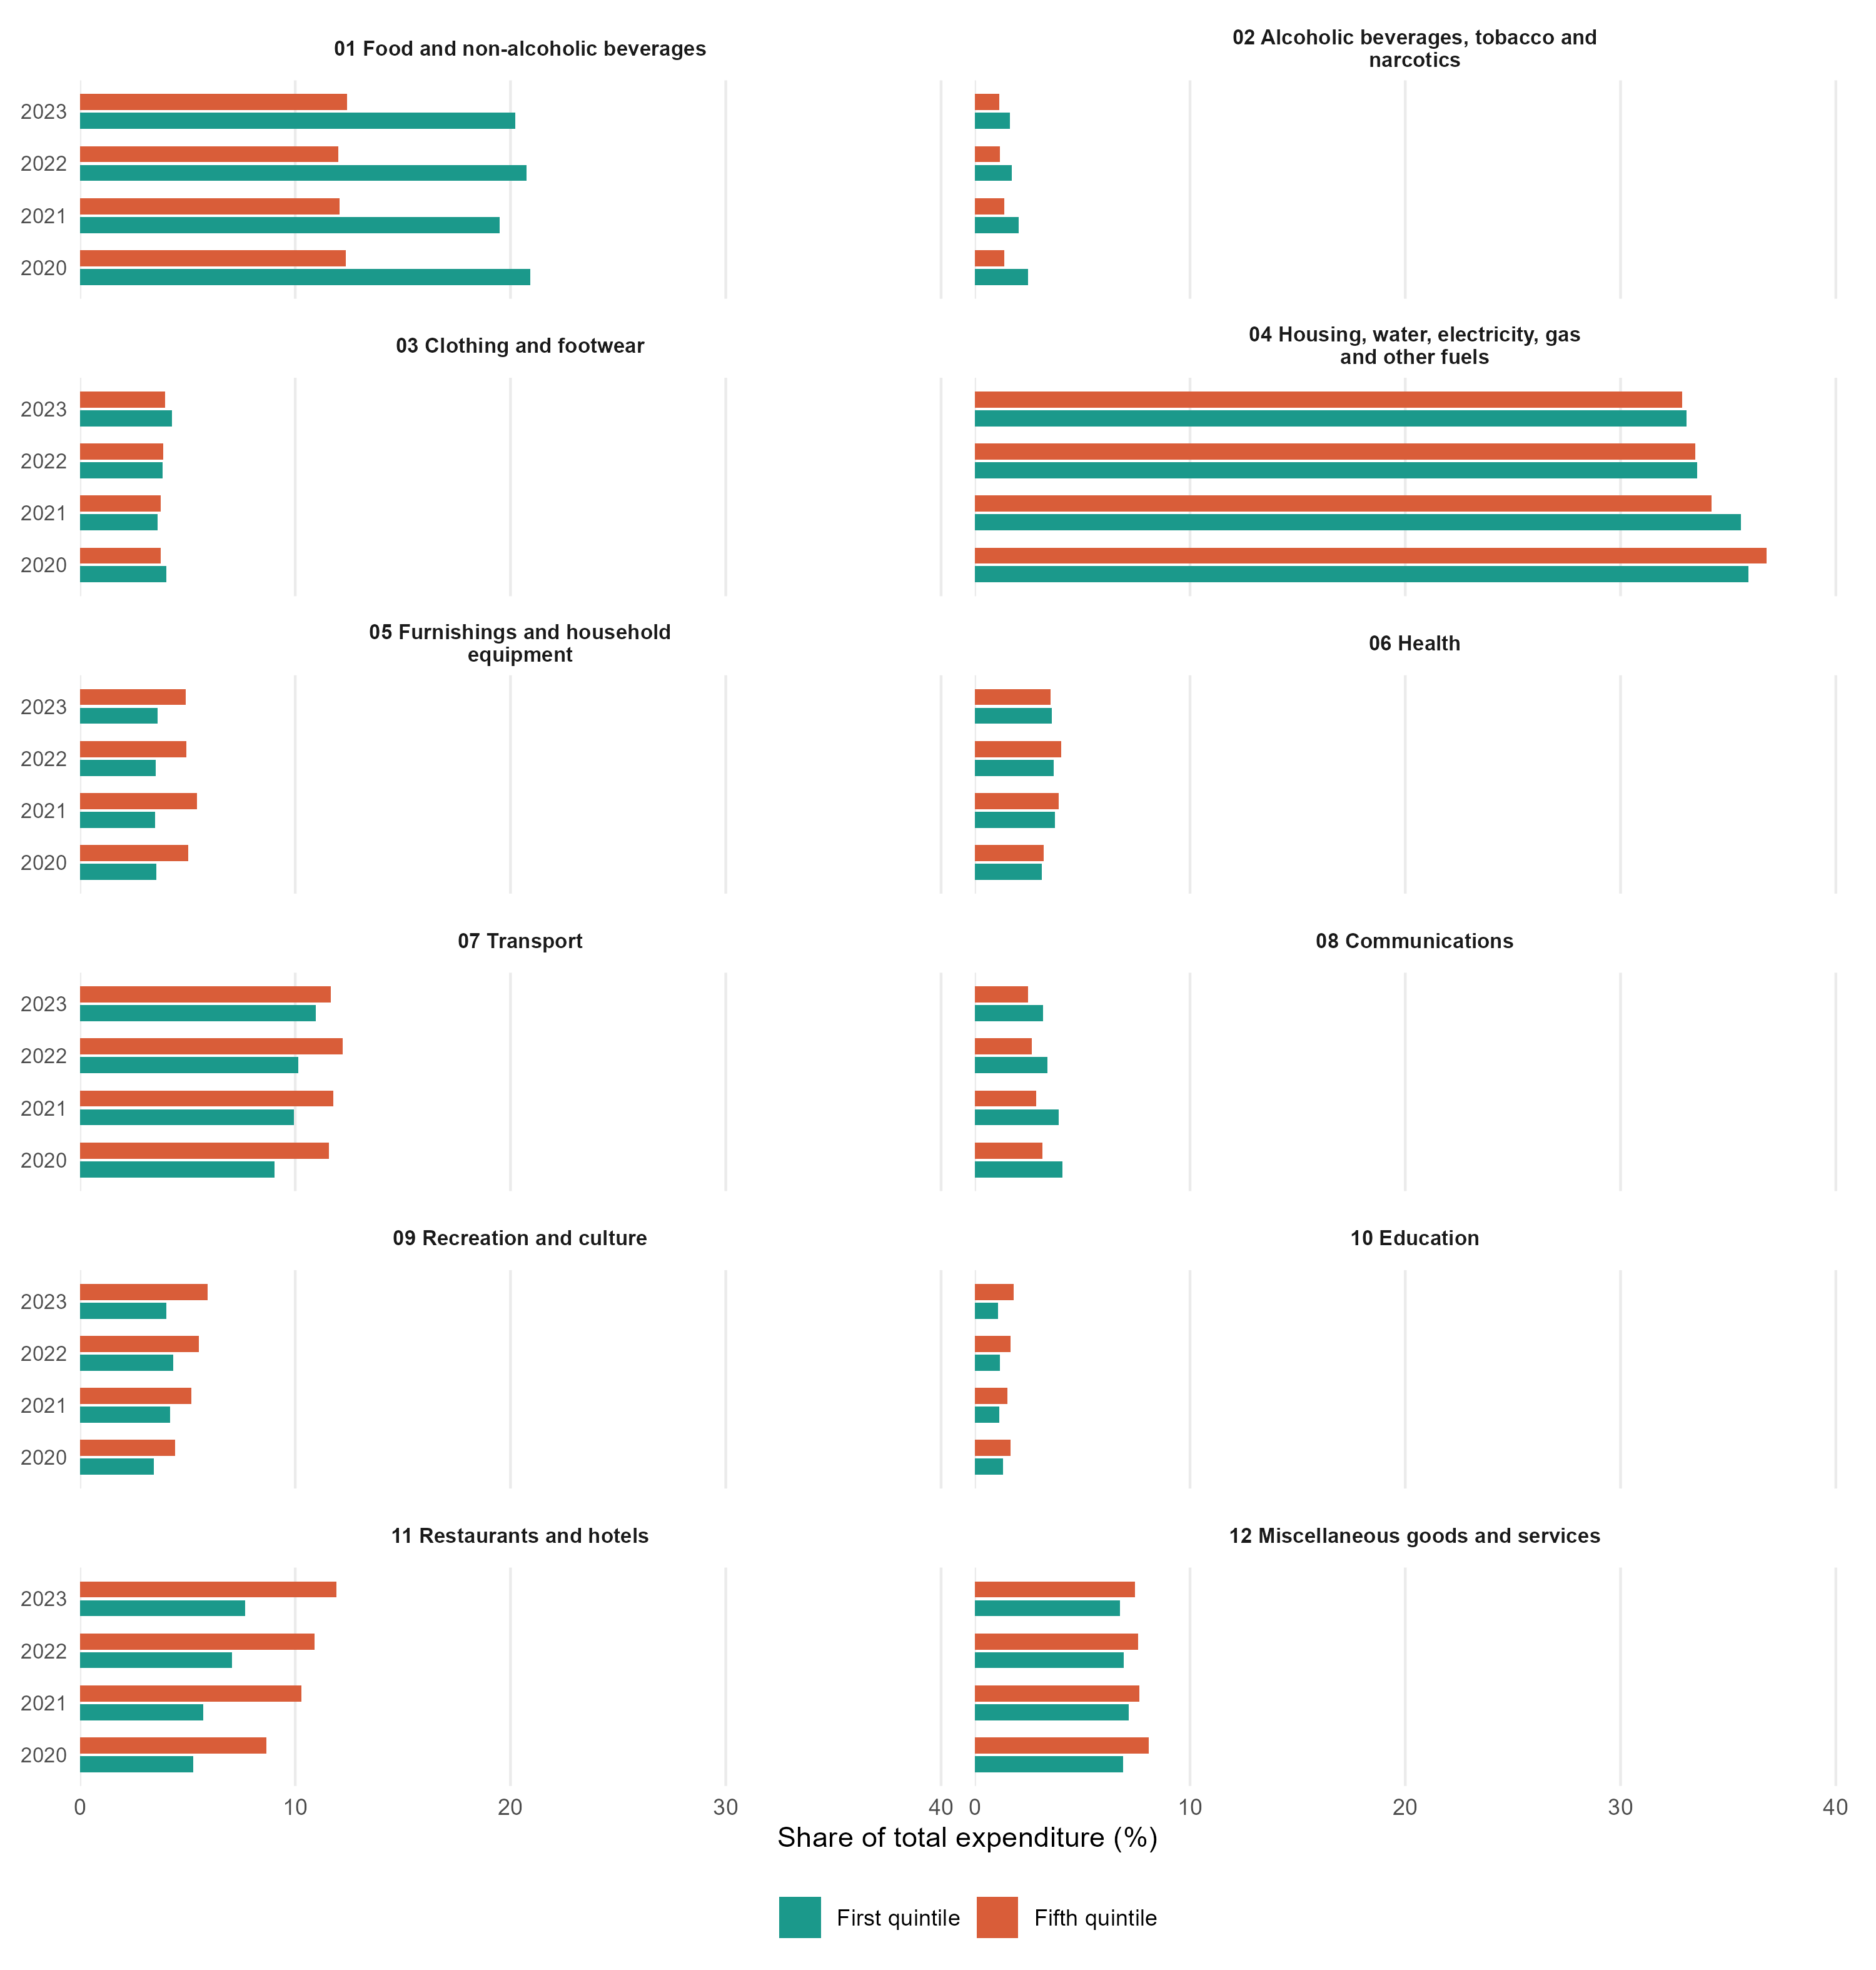
\includegraphics[width=0.98\textwidth,height=0.86\textheight,keepaspectratio]{fig/fig_ES_income_quintile_coicop_weights_2020_2023_grouped_bar.png}
\vspace{8pt}
\captionsetup{font=footnotesize, format=hang, singlelinecheck=false, justification=justified}
\caption*{Notes: The figure reports the share of each main COICOP category in total household expenditure for the first and fifth equivalised-income quintiles. Quintiles are computed separately by year using household weights.\\
Source: INE Encuesta de Presupuestos Familiares public-use microdata, authors' calculations.}
\end{figure}
%%%%%%%%%%%%%%%%%%%%%%%%%%%%%%%%%%%%%%%%%%%%%%%%%%%%%%%%%%%%%%
\newpage



%%%%%%%%%%%%%%%%%%%%%%%%%%%%%%%%%%%%%%%%%%%%%%%%%%%%%%%%%%%%%%
\begin{figure}[H]
\centering
\caption{Price indices by household group, France, COICOP level 3 (index, 1996 = 100)}
\label{fig:app-fr-level3-price-indices}
\begin{subfigure}{0.88\textwidth}
  \centering
  \caption{Income quintiles}
  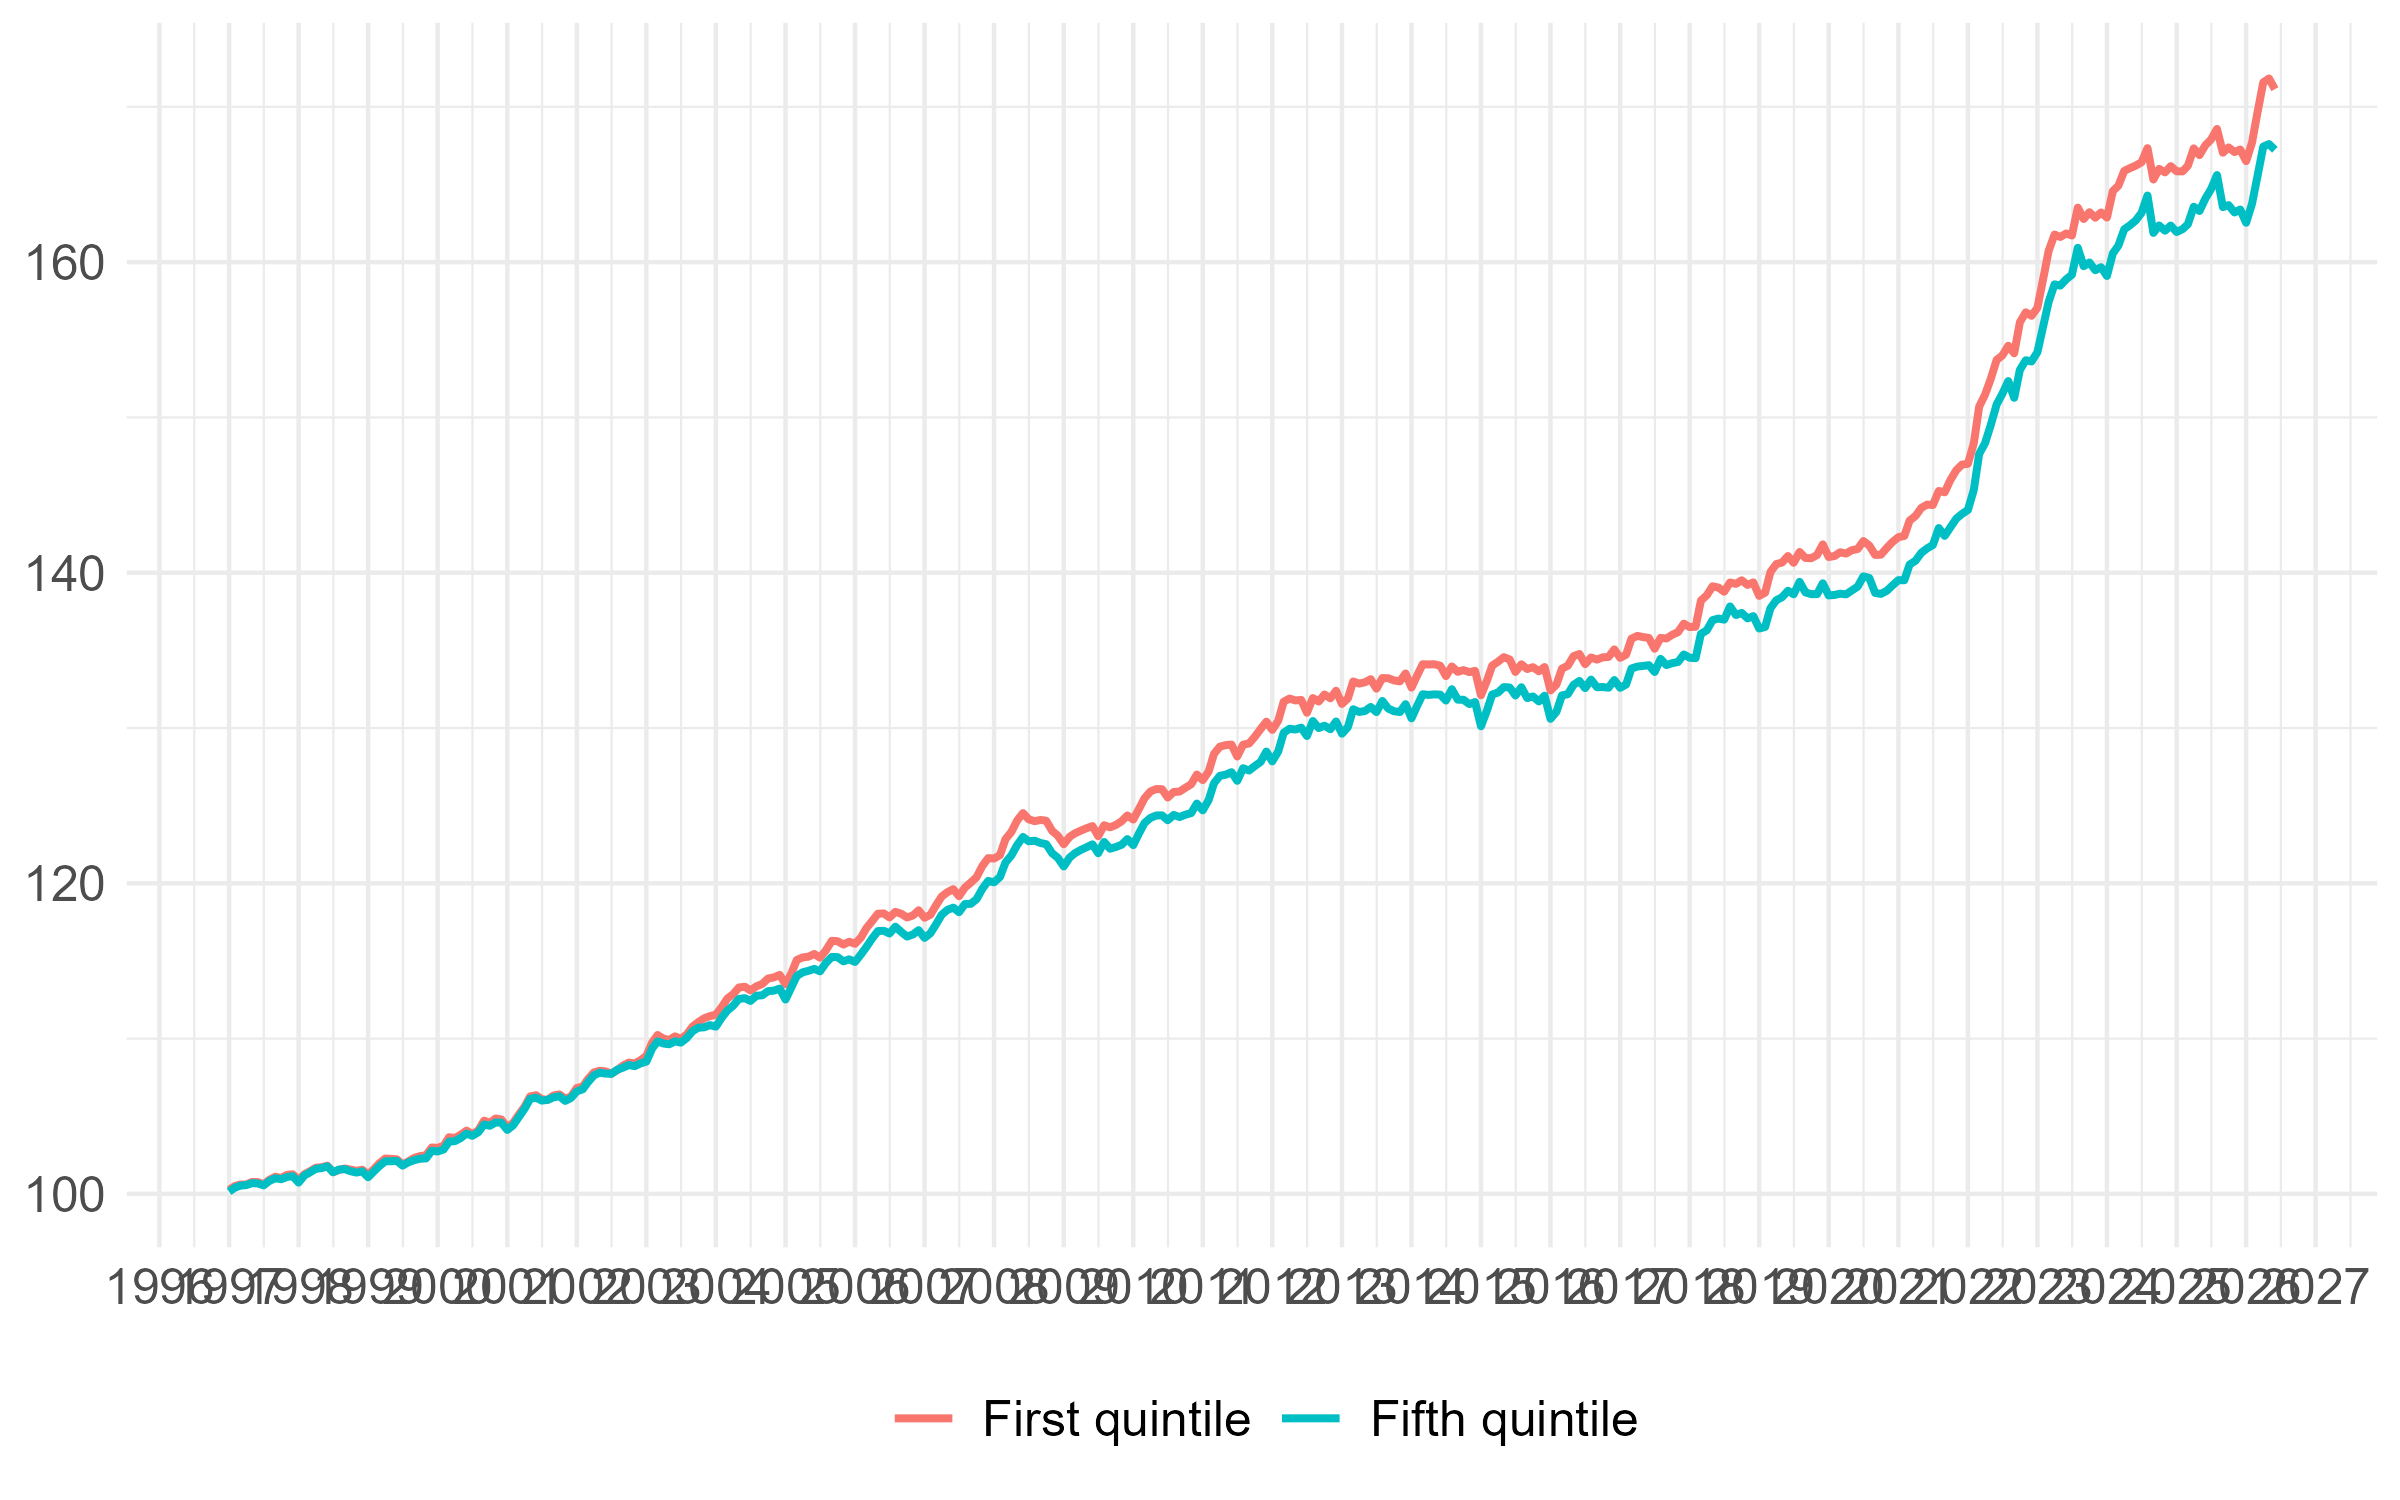
\includegraphics[width=\linewidth,height=0.22\textheight,keepaspectratio]{fig/fig_FR_1996_2026_income_price_index_level3_Q1_Q5.png}
\end{subfigure}

\vspace{6pt}

\begin{subfigure}{0.88\textwidth}
  \centering
  \caption{Age groups}
  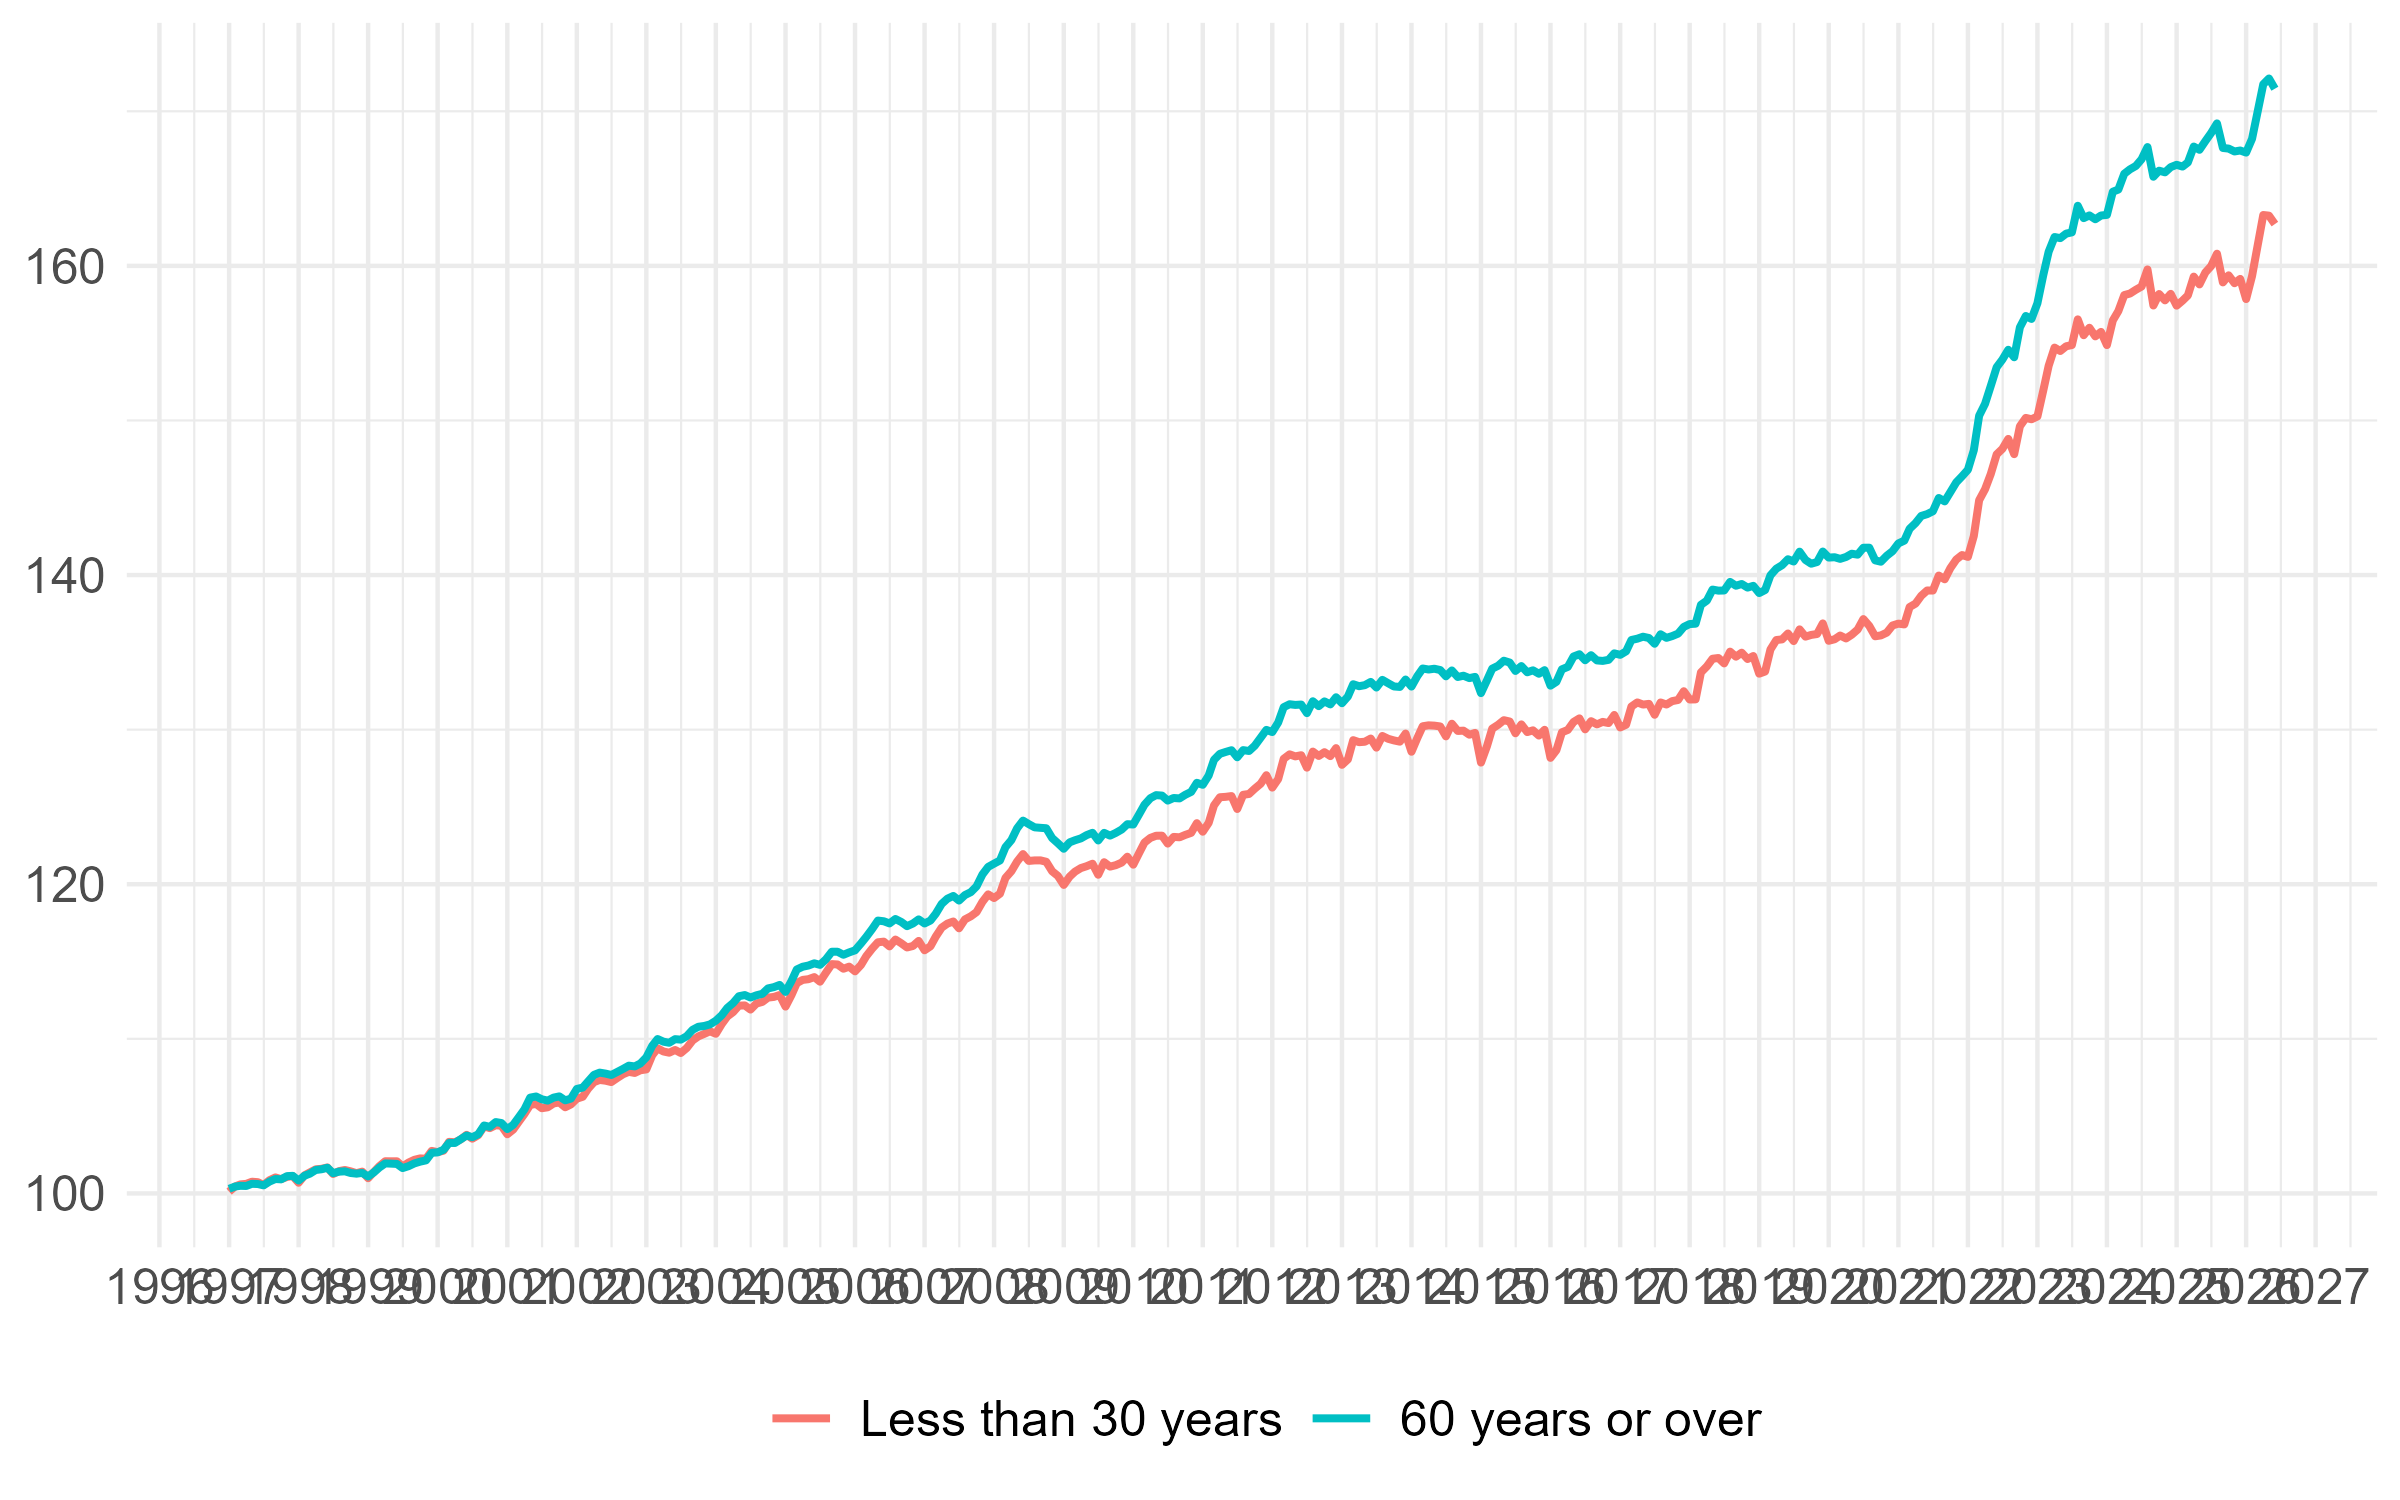
\includegraphics[width=\linewidth,height=0.22\textheight,keepaspectratio]{fig/fig_FR_1996_2026_age_price_index_level3_young_old.png}
\end{subfigure}

\vspace{6pt}

\begin{subfigure}{0.88\textwidth}
  \centering
  \caption{Residence area}
  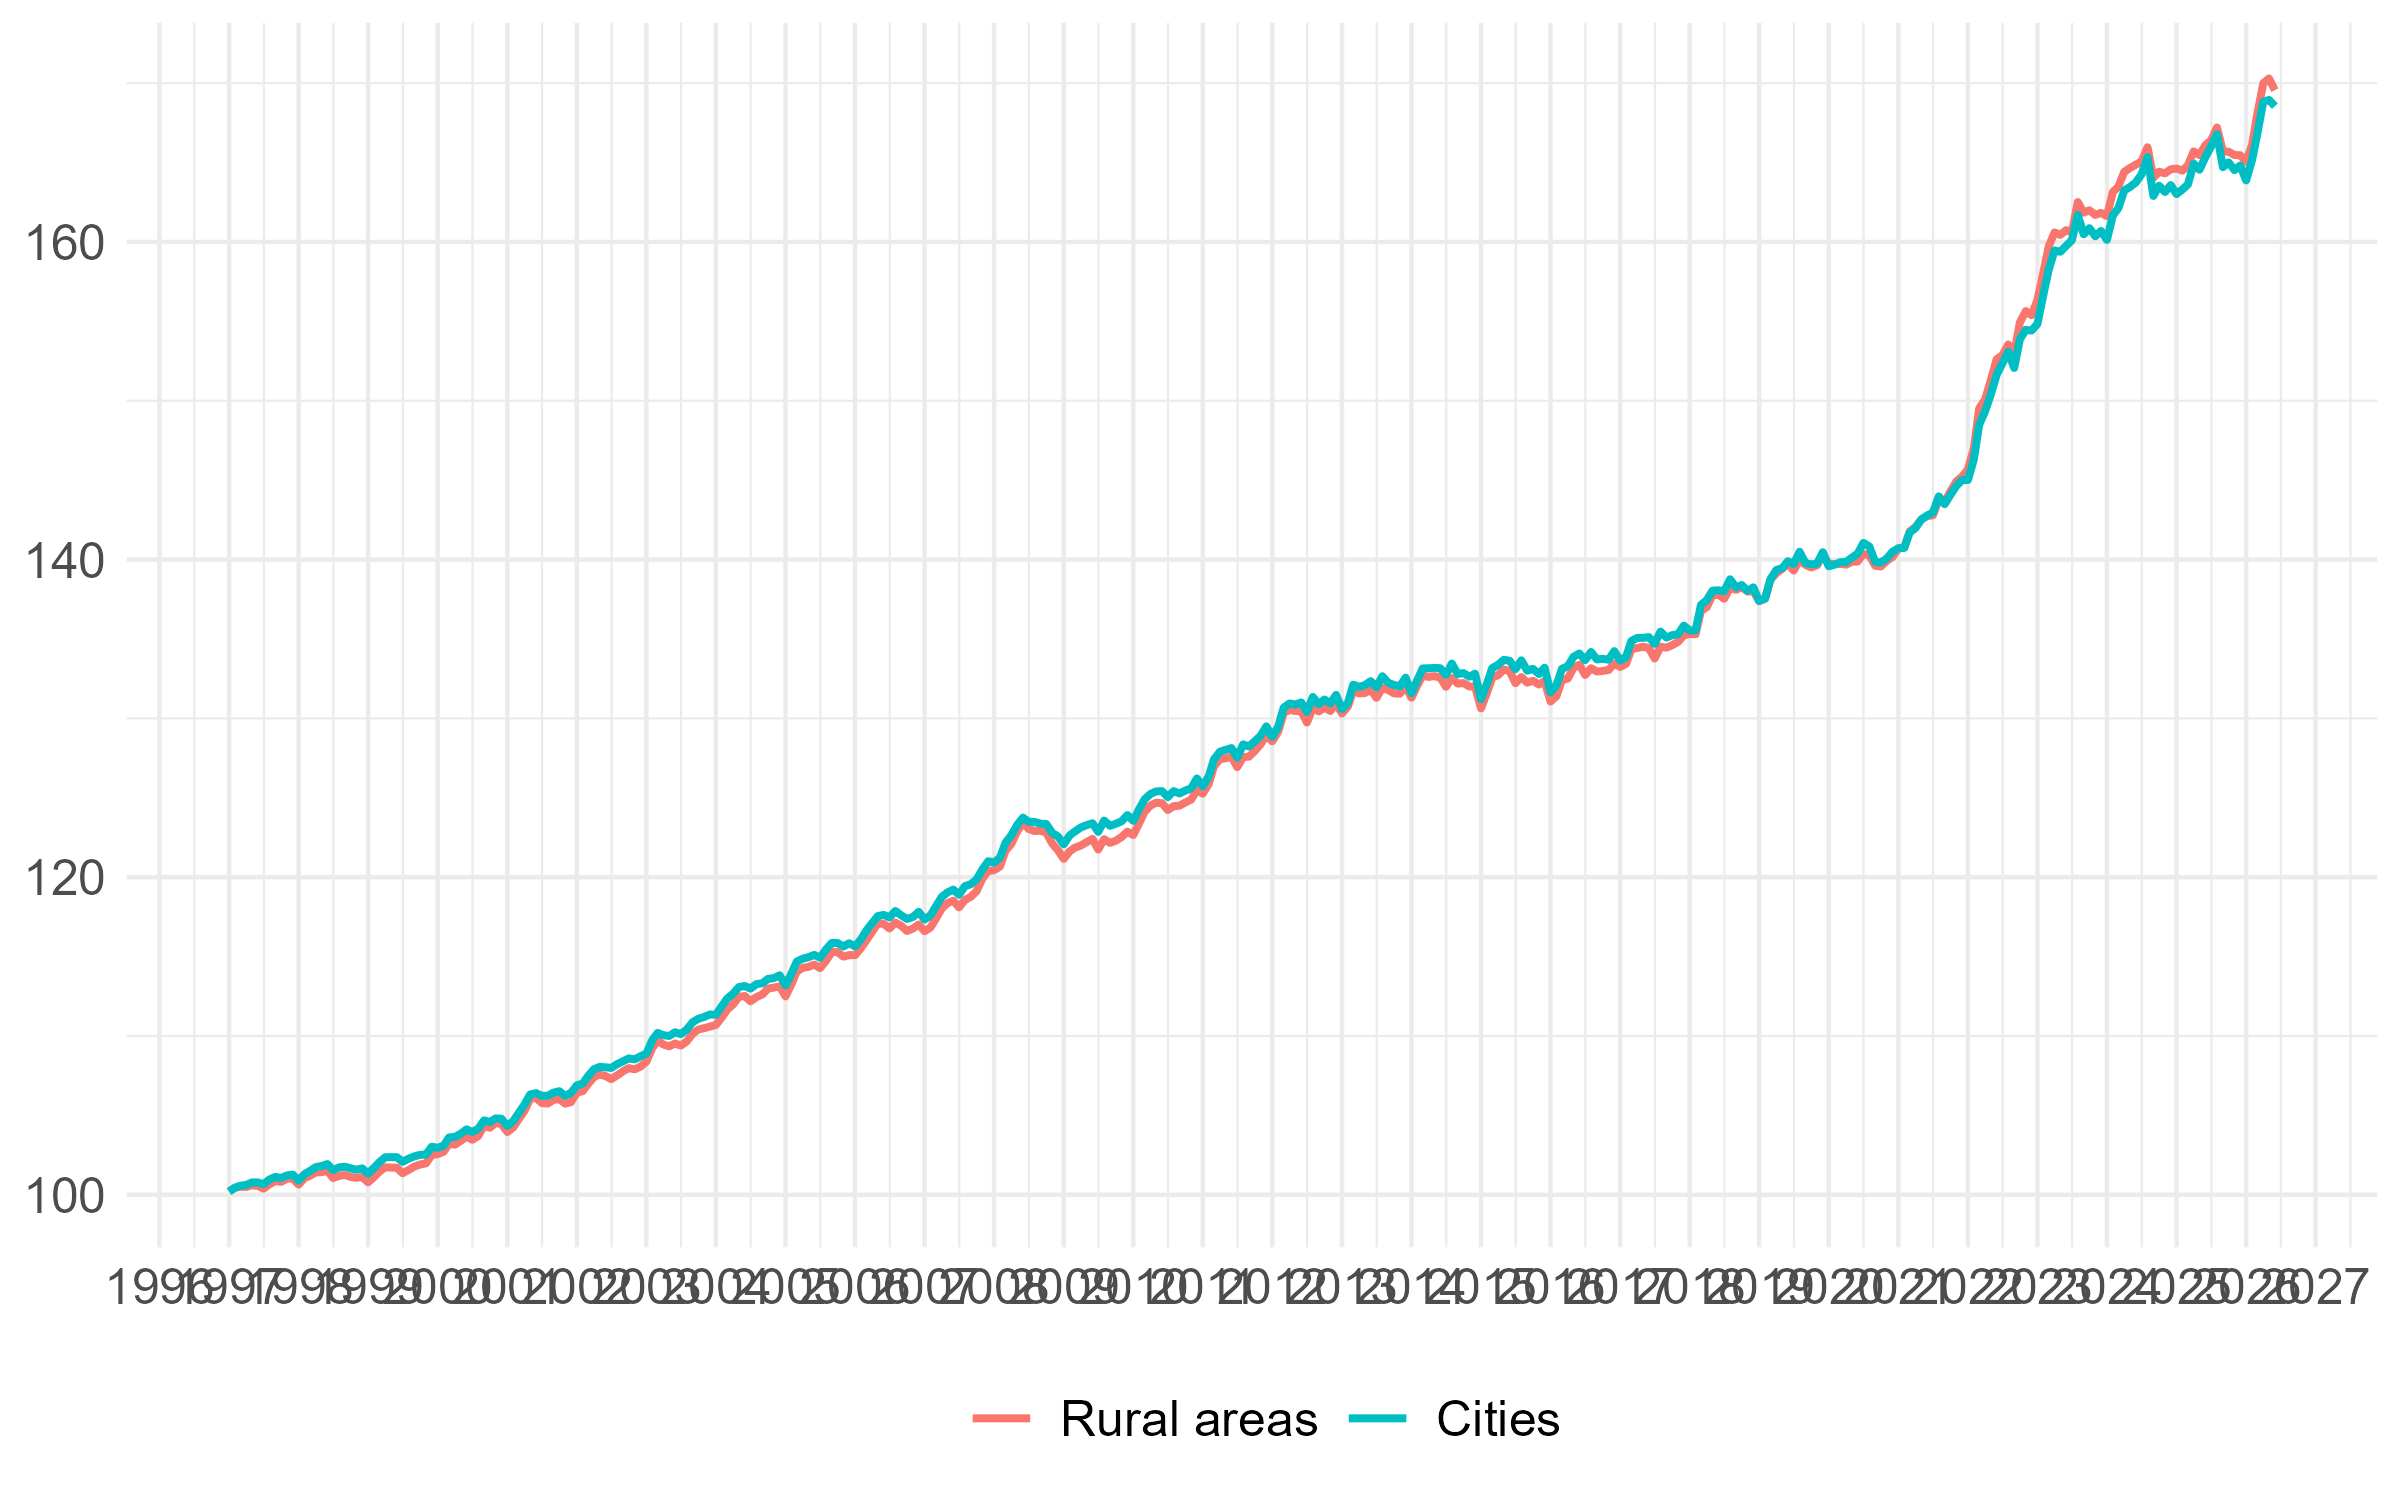
\includegraphics[width=\linewidth,height=0.22\textheight,keepaspectratio]{fig/fig_FR_1996_2026_urban_price_index_level3_rural_paris.png}
\end{subfigure}
\vspace{10pt}
\captionsetup{font=footnotesize, format=hang, singlelinecheck=false, justification=justified}
\caption*{Notes: The figure reports chained price indices from 1996 using the France level-3 workflow. The panels compare income quintiles, age groups, and residence areas.\\
Sources: Eurostat HICP; INSEE HBS 2017; authors' calculations.}
\end{figure}
%%%%%%%%%%%%%%%%%%%%%%%%%%%%%%%%%%%%%%%%%%%%%%%%%%%%%%%%%%%%%%
\newpage

%%%%%%%%%%%%%%%%%%%%%%%%%%%%%%%%%%%%%%%%%%%%%%%%%%%%%%%%%%%%%%
\begin{figure}[H]
\centering
\caption{Inflation by household group, France, COICOP level 3 (in \%)}
\label{fig:app-fr-level3-inflation}
\begin{subfigure}{0.88\textwidth}
  \centering
  \caption{Income quintiles}
  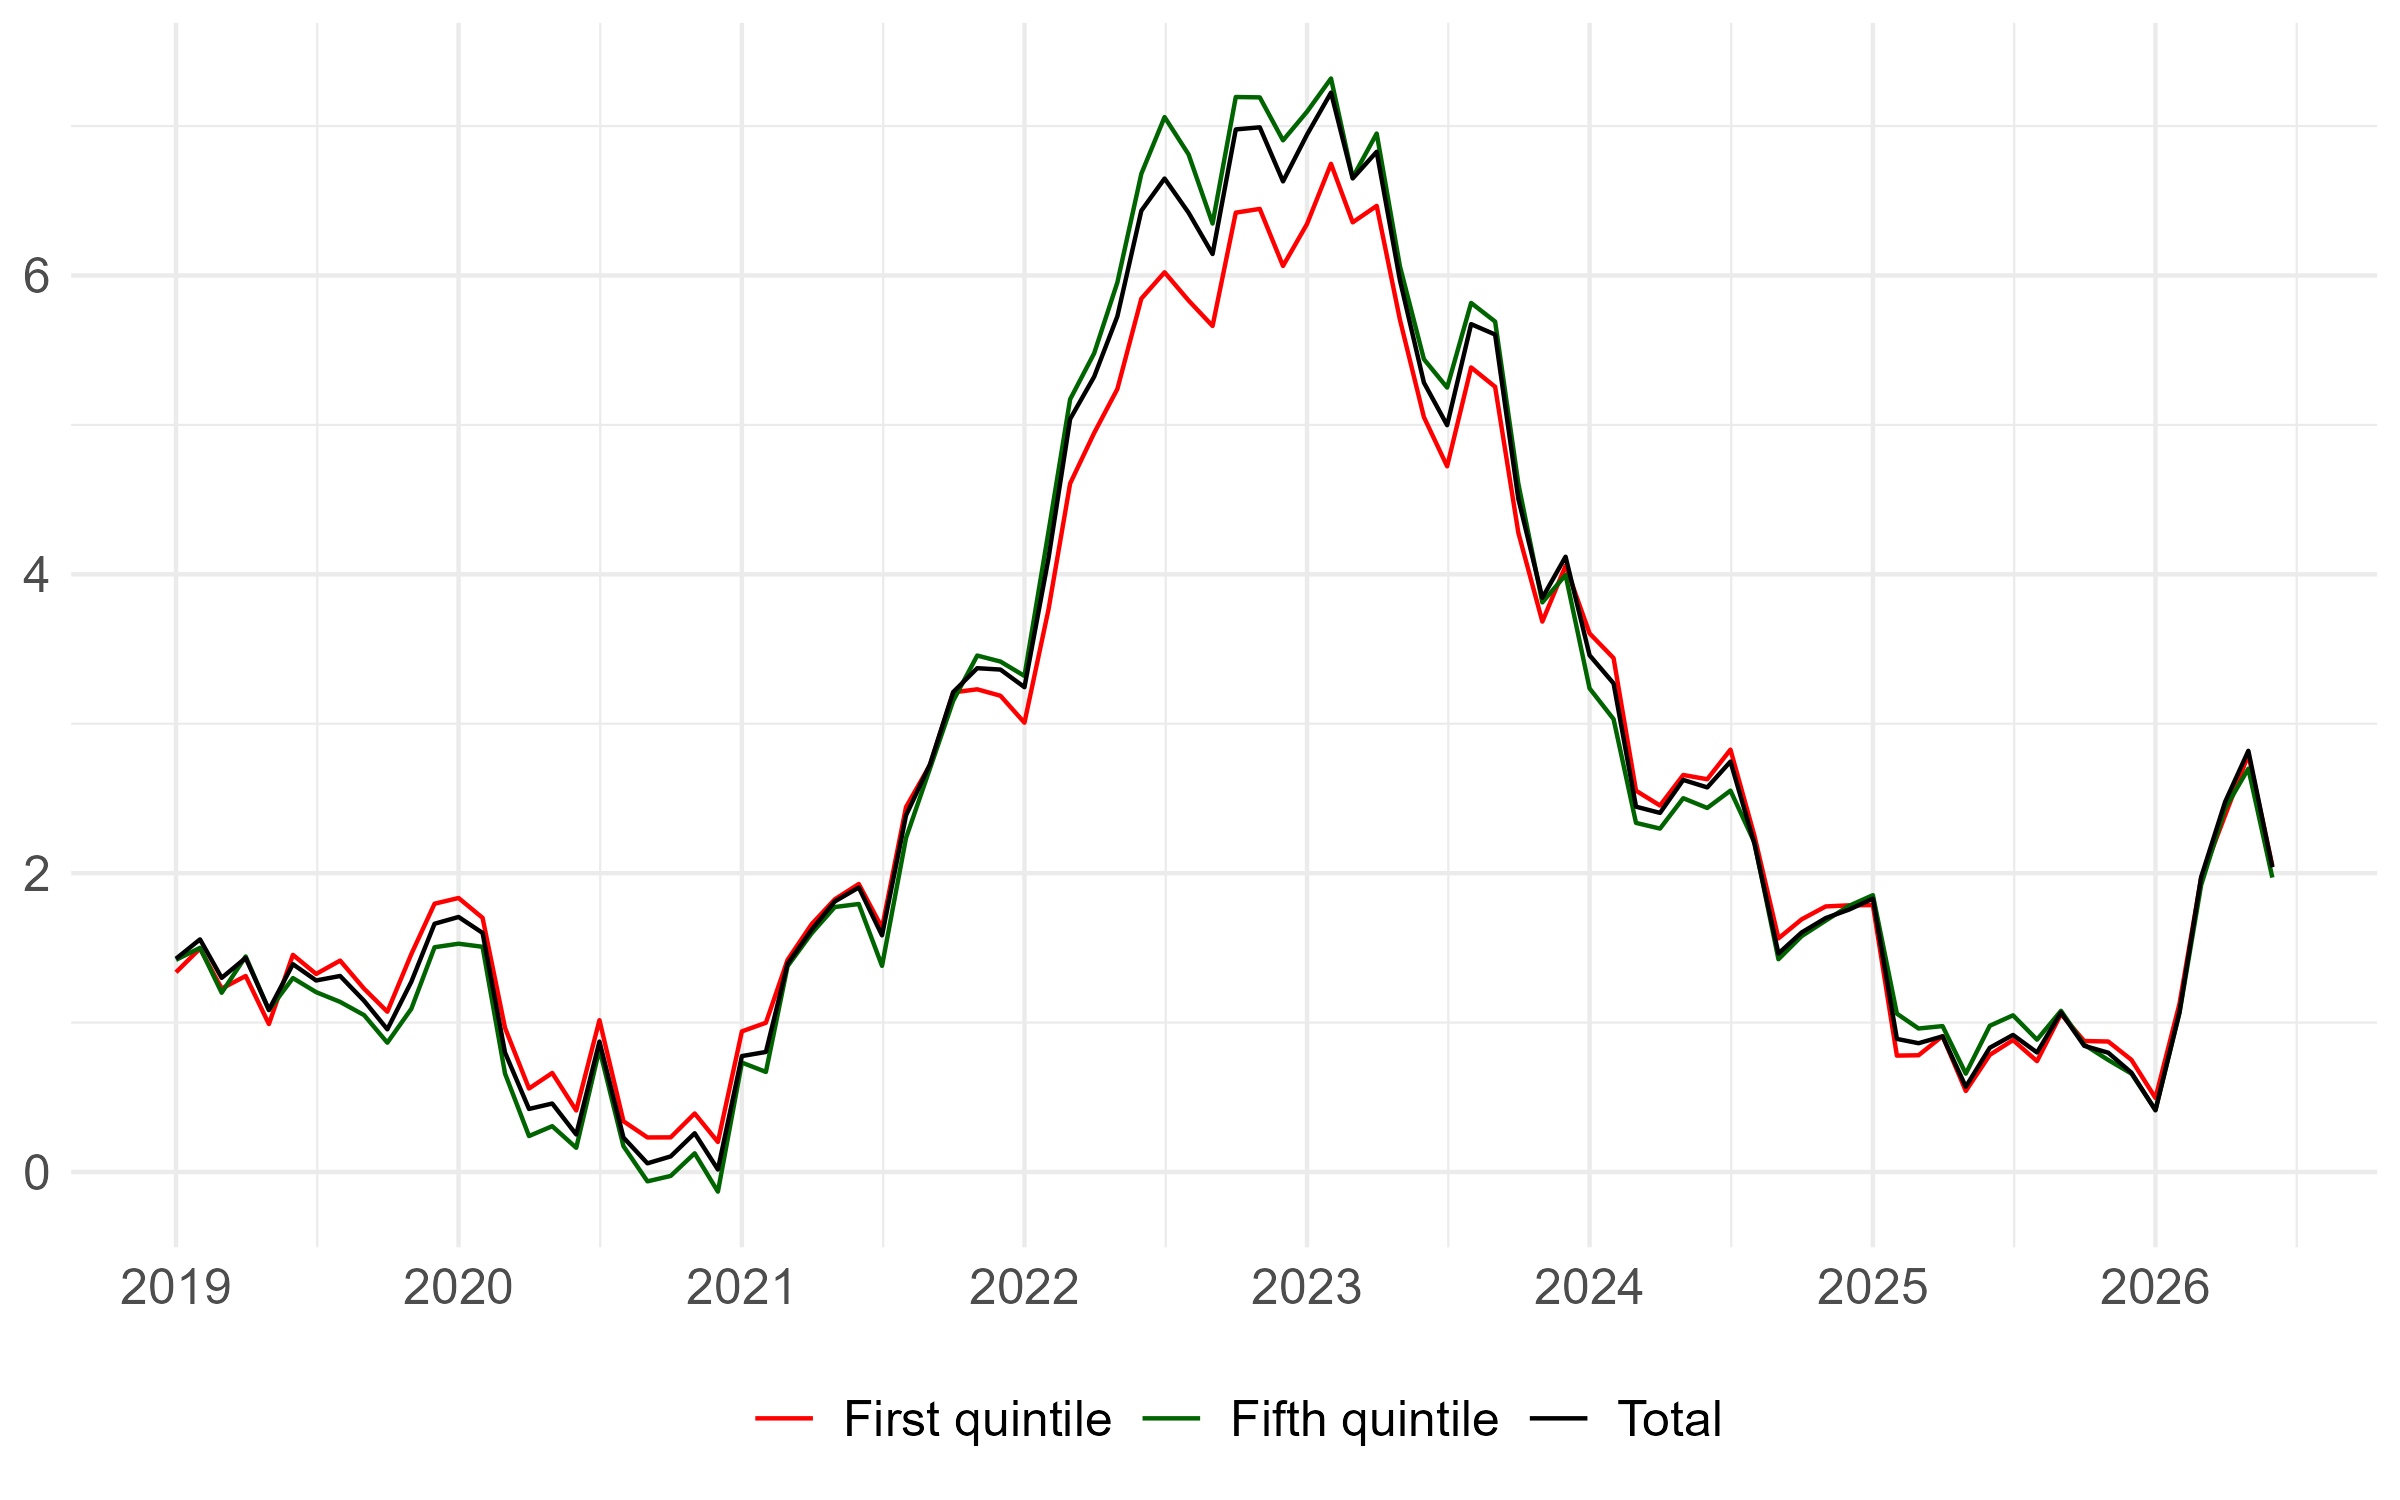
\includegraphics[width=\linewidth,height=0.22\textheight,keepaspectratio]{fig/fig_FR_2019_2026_income_inflation_level3_Q1_Q5.png}
\end{subfigure}

\vspace{6pt}

\begin{subfigure}{0.88\textwidth}
  \centering
  \caption{Age groups}
  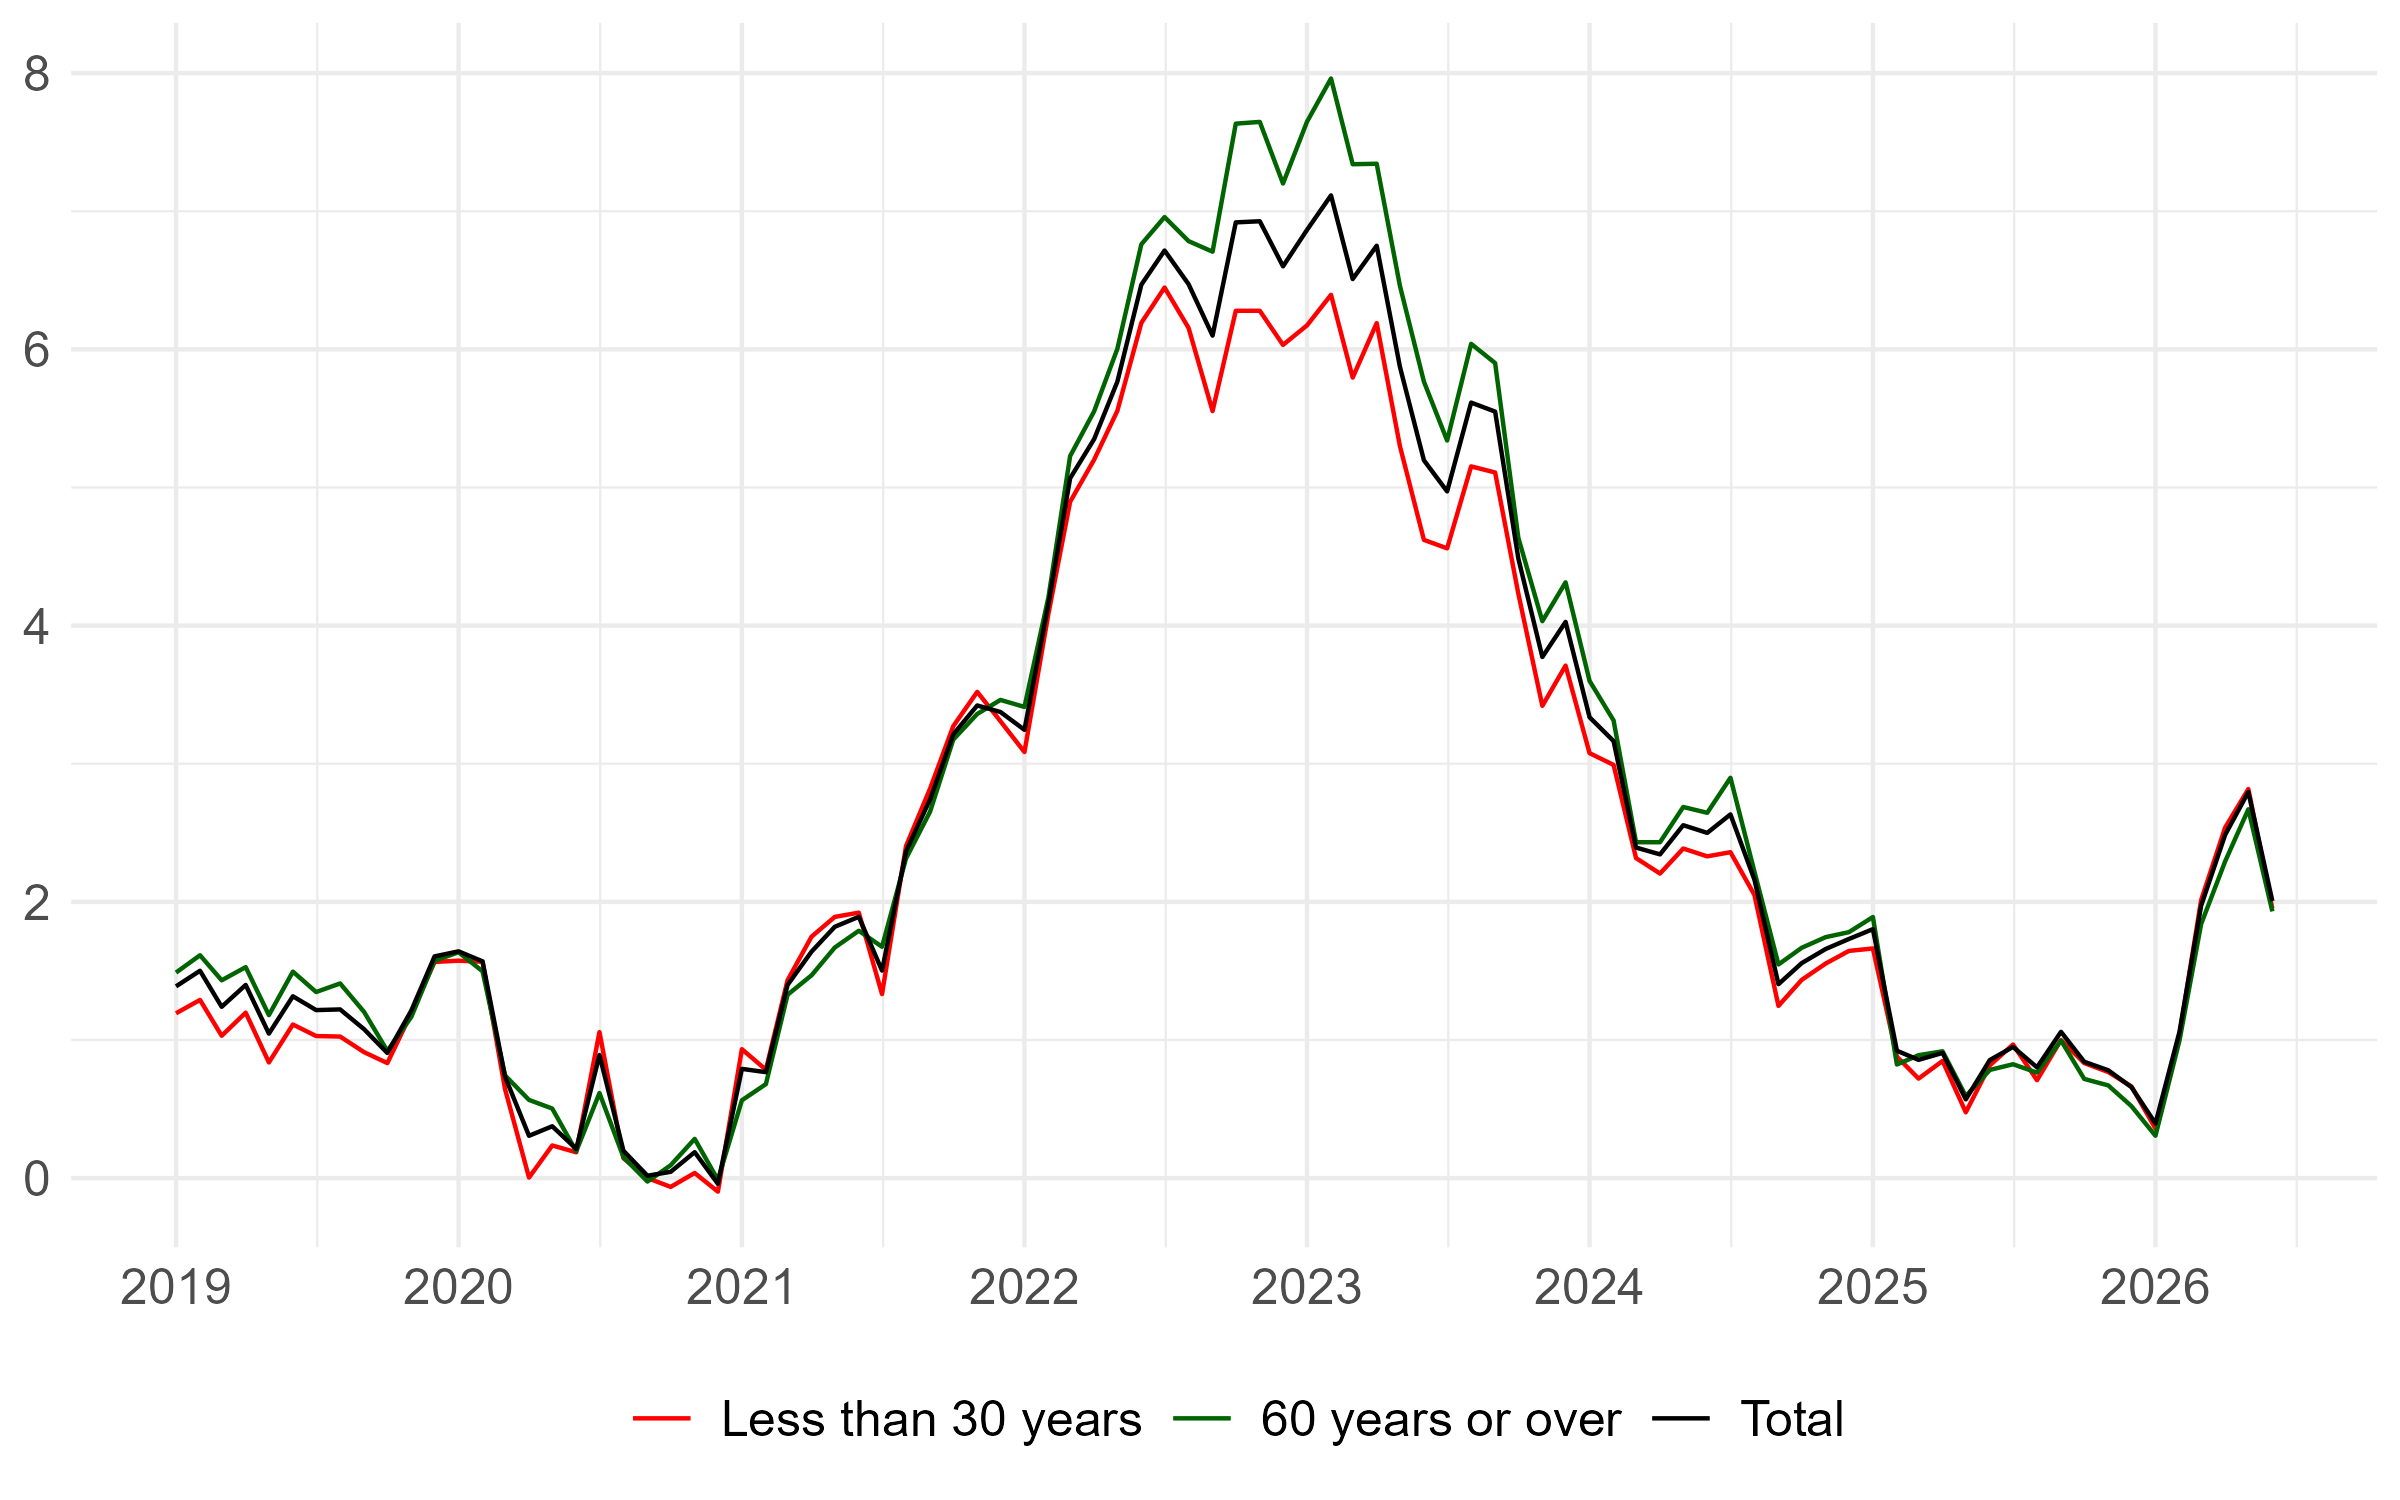
\includegraphics[width=\linewidth,height=0.22\textheight,keepaspectratio]{fig/fig_FR_2019_2026_age_inflation_level3_under25_65plus.png}
\end{subfigure}

\vspace{6pt}

\begin{subfigure}{0.88\textwidth}
  \centering
  \caption{Residence area}
  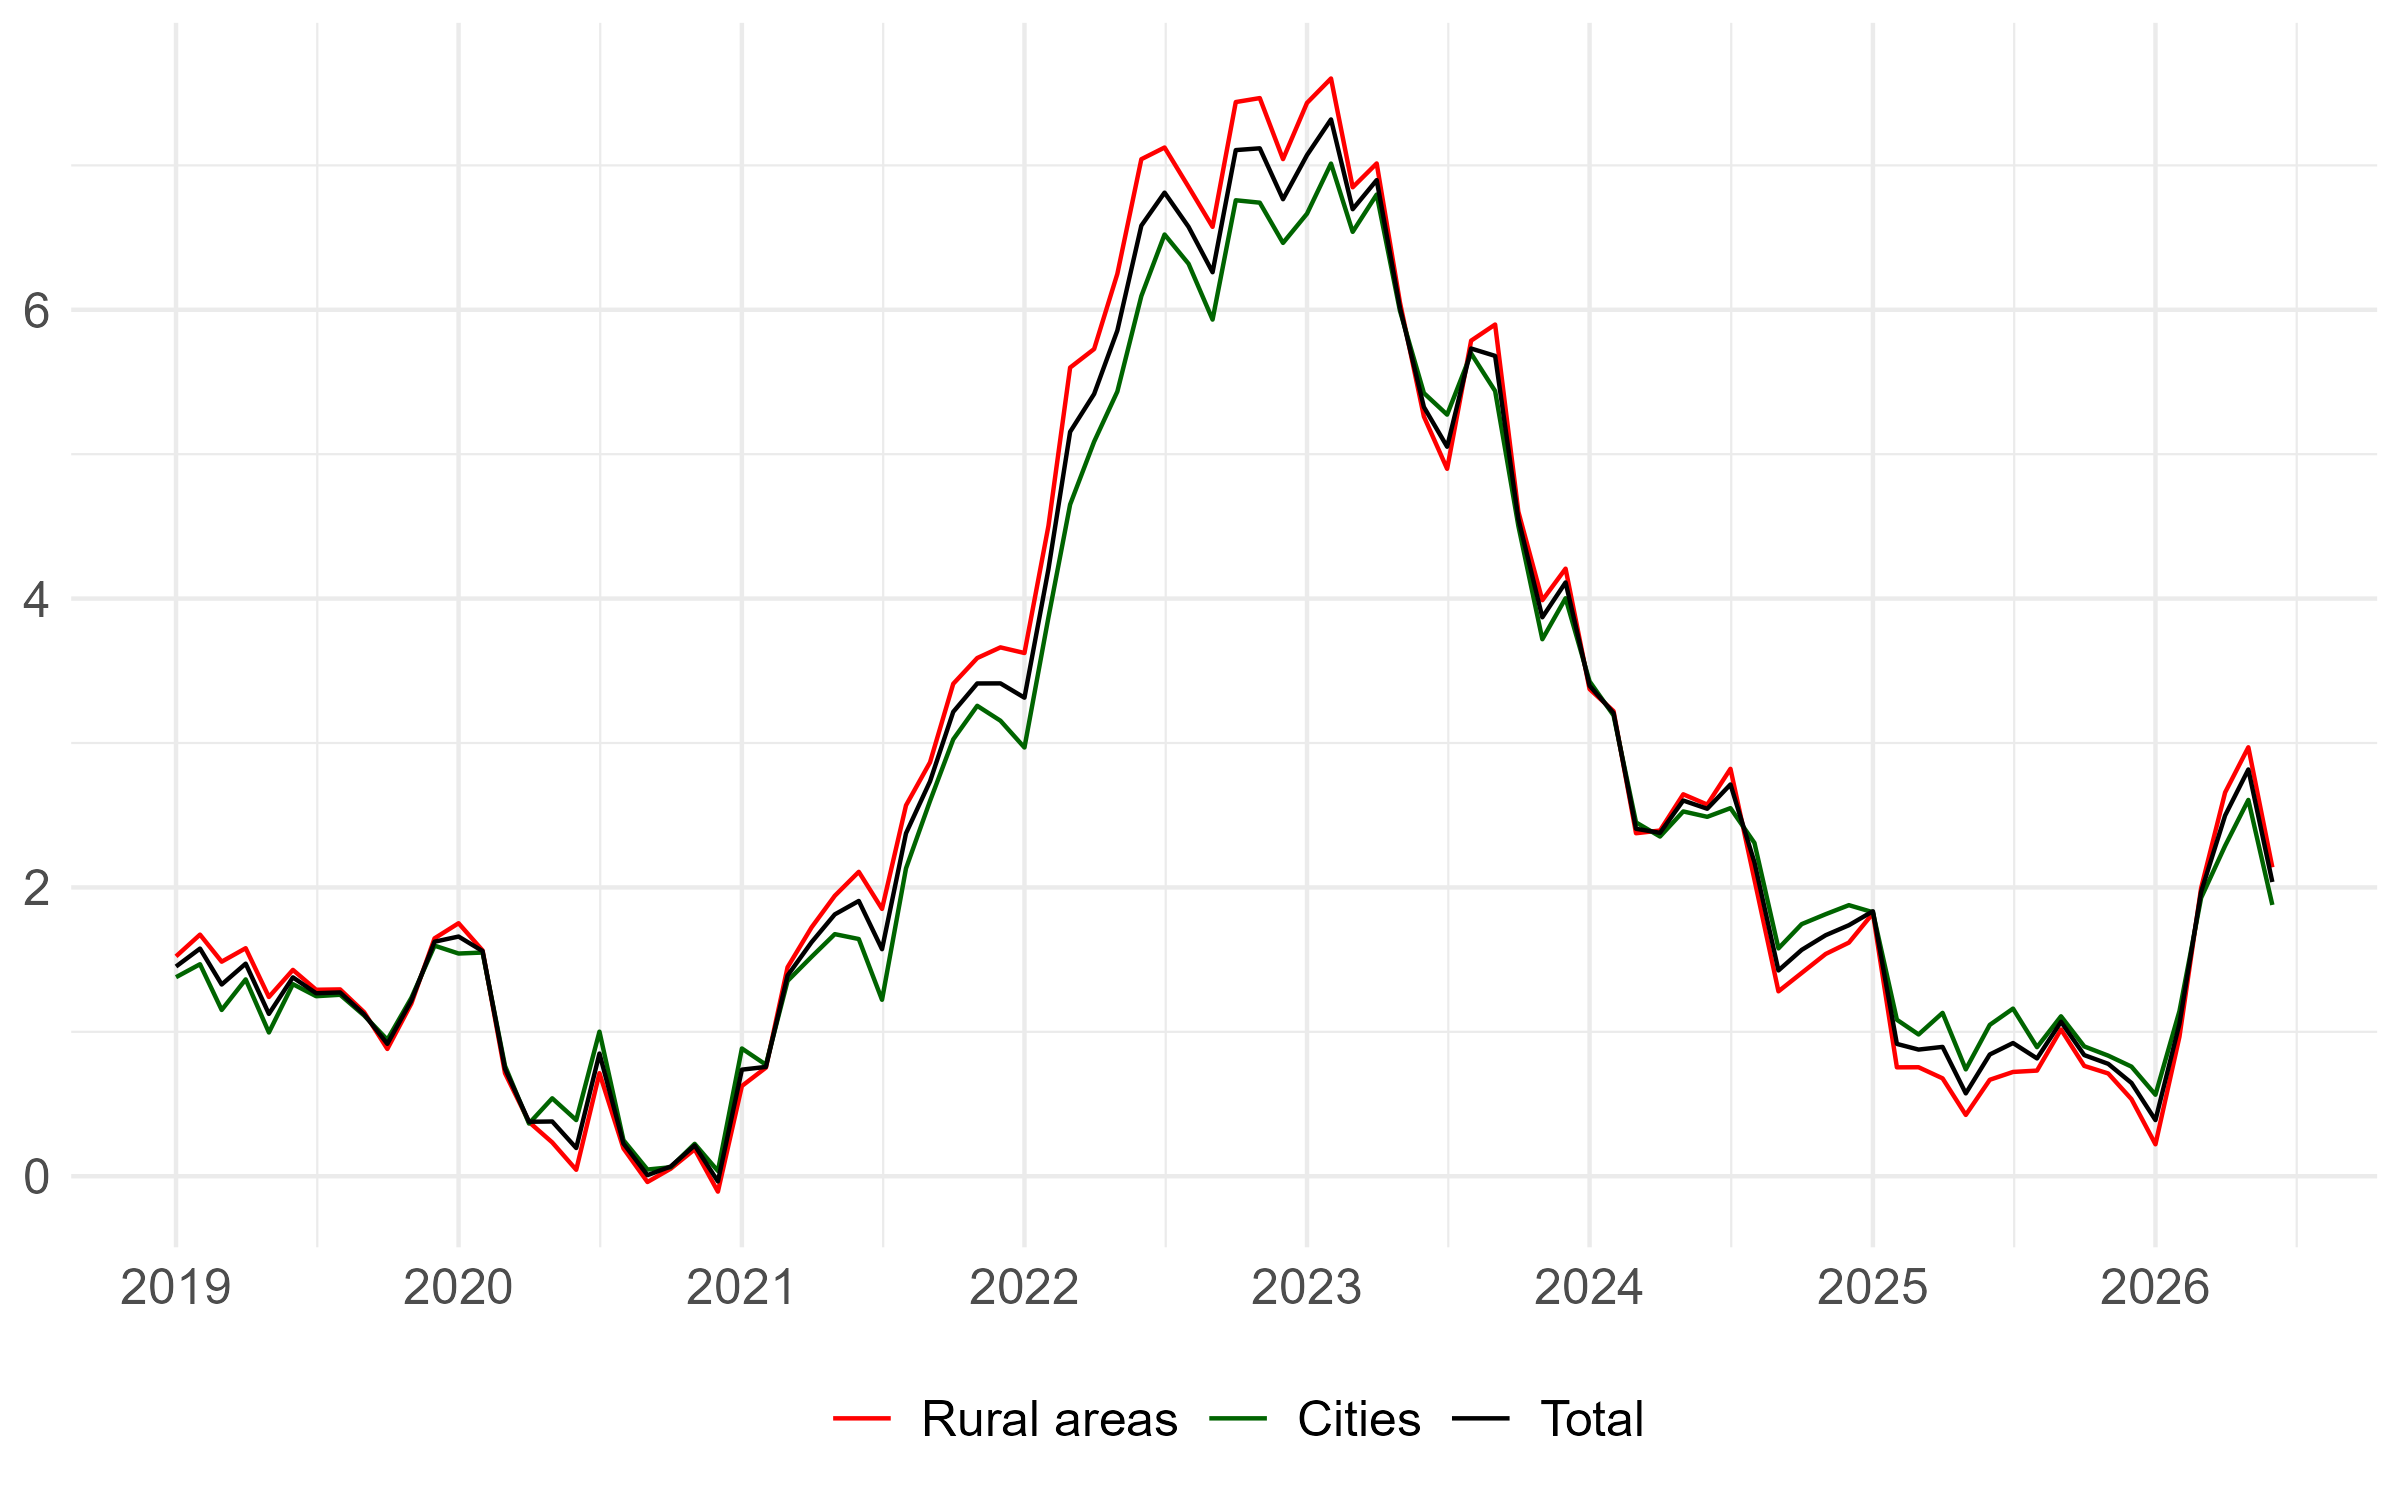
\includegraphics[width=\linewidth,height=0.22\textheight,keepaspectratio]{fig/fig_FR_2019_2026_urban_inflation_level3_rural_paris.png}
\end{subfigure}
\vspace{10pt}
\captionsetup{font=footnotesize, format=hang, singlelinecheck=false, justification=justified}
\caption*{Notes: The figure reports monthly year-on-year inflation rates using the France level-3 workflow. The panels compare income quintiles, age groups, and residence areas over the recent inflation episode.\\
Sources: Eurostat HICP; INSEE HBS 2017; authors' calculations.}
\end{figure}
%%%%%%%%%%%%%%%%%%%%%%%%%%%%%%%%%%%%%%%%%%%%%%%%%%%%%%%%%%%%%%
\newpage

%%%%%%%%%%%%%%%%%%%%%%%%%%%%%%%%%%%%%%%%%%%%%%%%%%%%%%%%%%%%%%
\begin{figure}[H]
\centering
\caption{Contributions to inflation gaps, France, COICOP level 3 (in pp)}
\label{fig:app-fr-level3-contributions}
\begin{subfigure}{0.88\textwidth}
  \centering
  \caption{Income gap: Quintile 1 minus Quintile 5}
  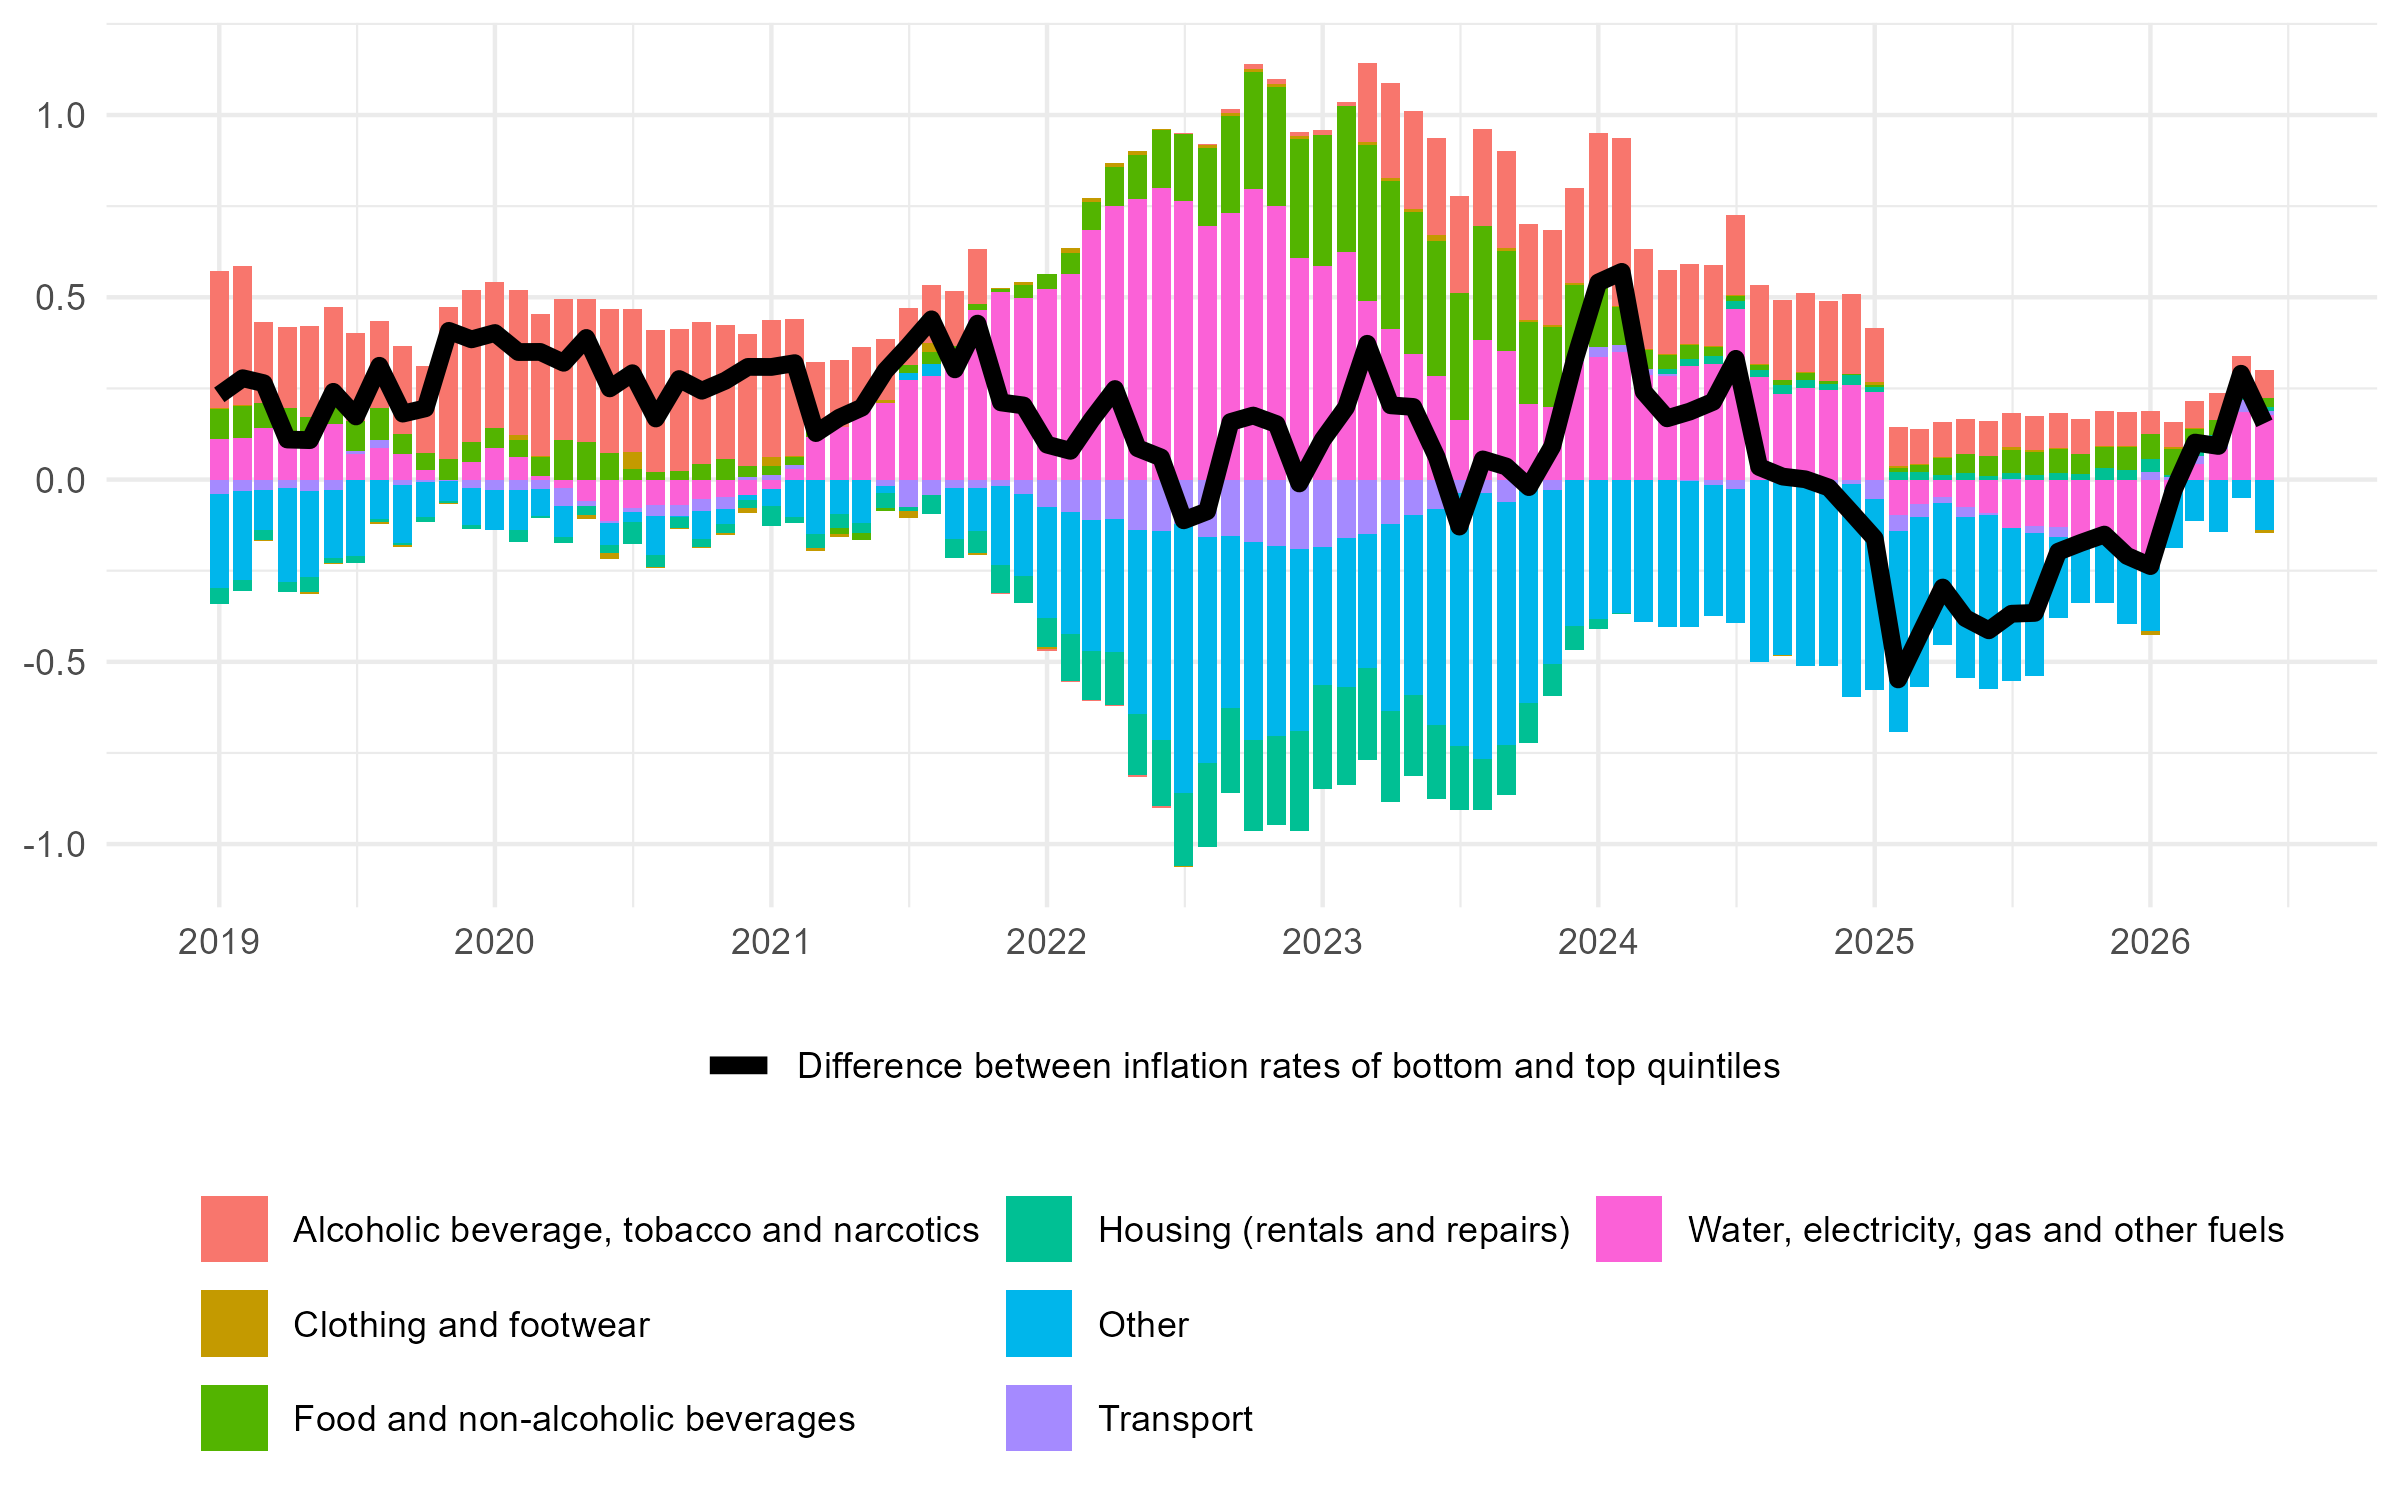
\includegraphics[width=\linewidth,height=0.22\textheight,keepaspectratio]{fig/fig_FR_2019_2026_income_contribution_gap_level3_Q1_Q5.png}
\end{subfigure}

\vspace{6pt}

\begin{subfigure}{0.88\textwidth}
  \centering
  \caption{Age gap: 65 years or over minus under 25}
  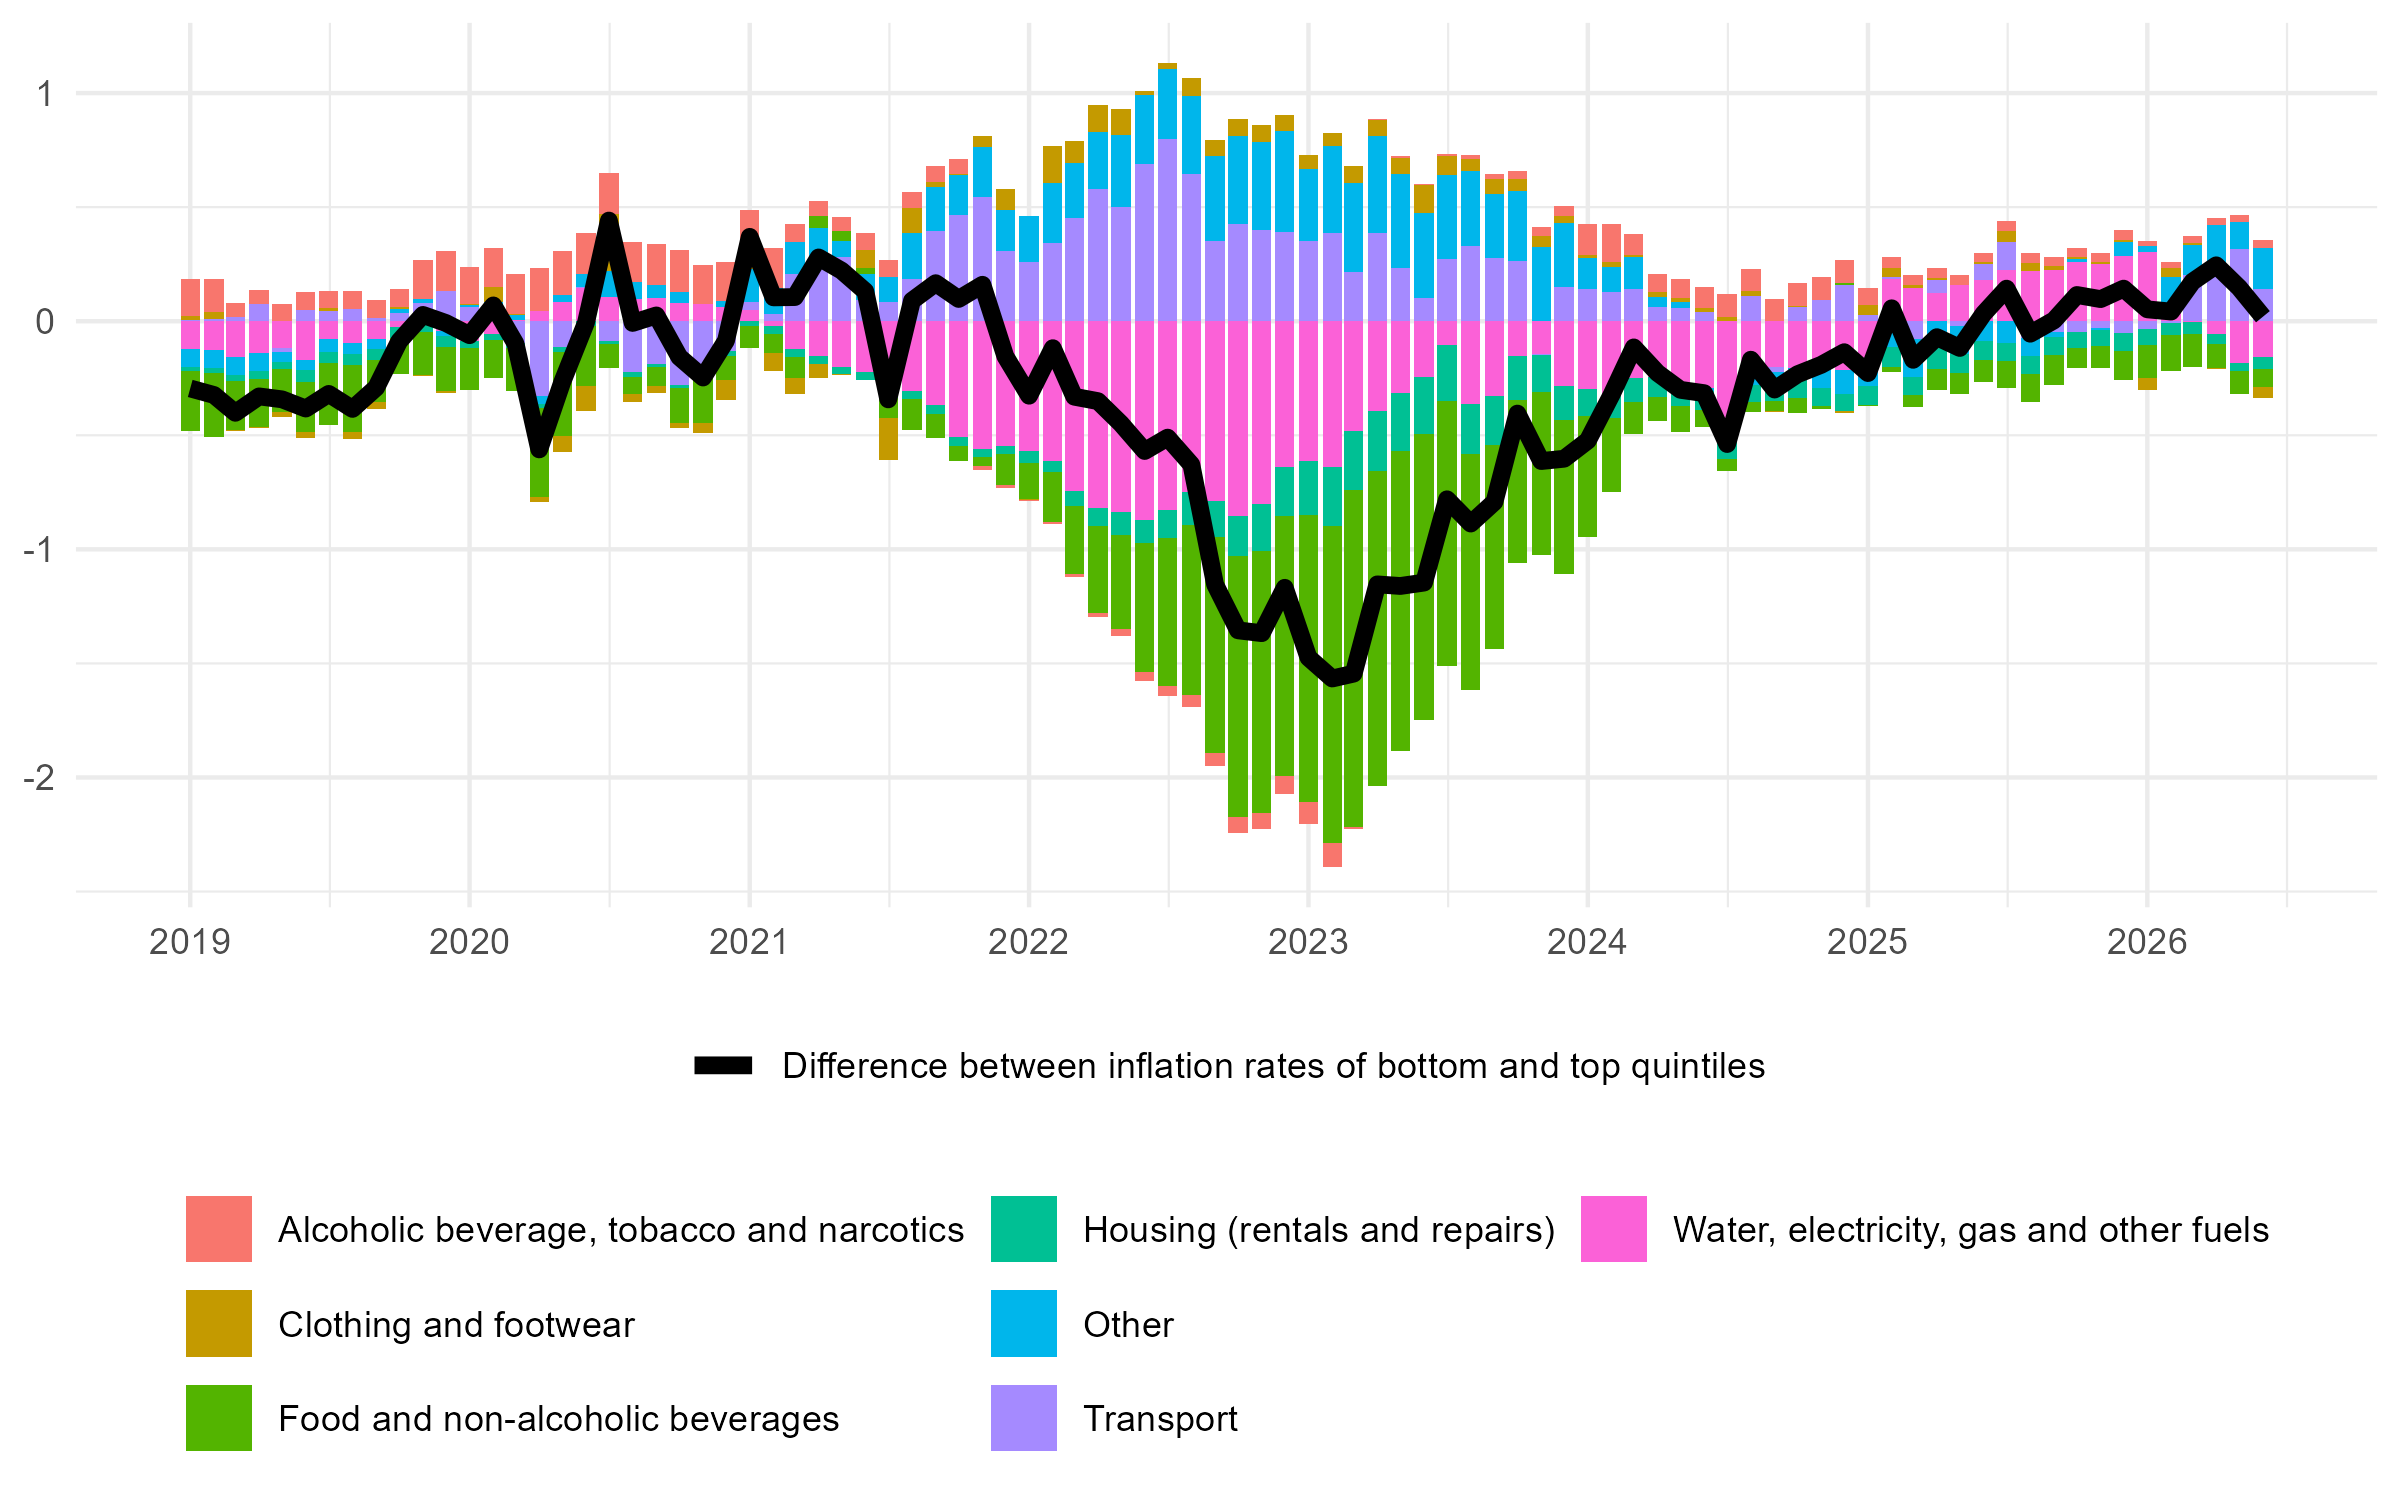
\includegraphics[width=\linewidth,height=0.22\textheight,keepaspectratio]{fig/fig_FR_2019_2026_age_contribution_gap_level3_65plus_under25.png}
\end{subfigure}

\vspace{6pt}

\begin{subfigure}{0.88\textwidth}
  \centering
  \caption{Residence-area gap: rural areas minus Paris}
  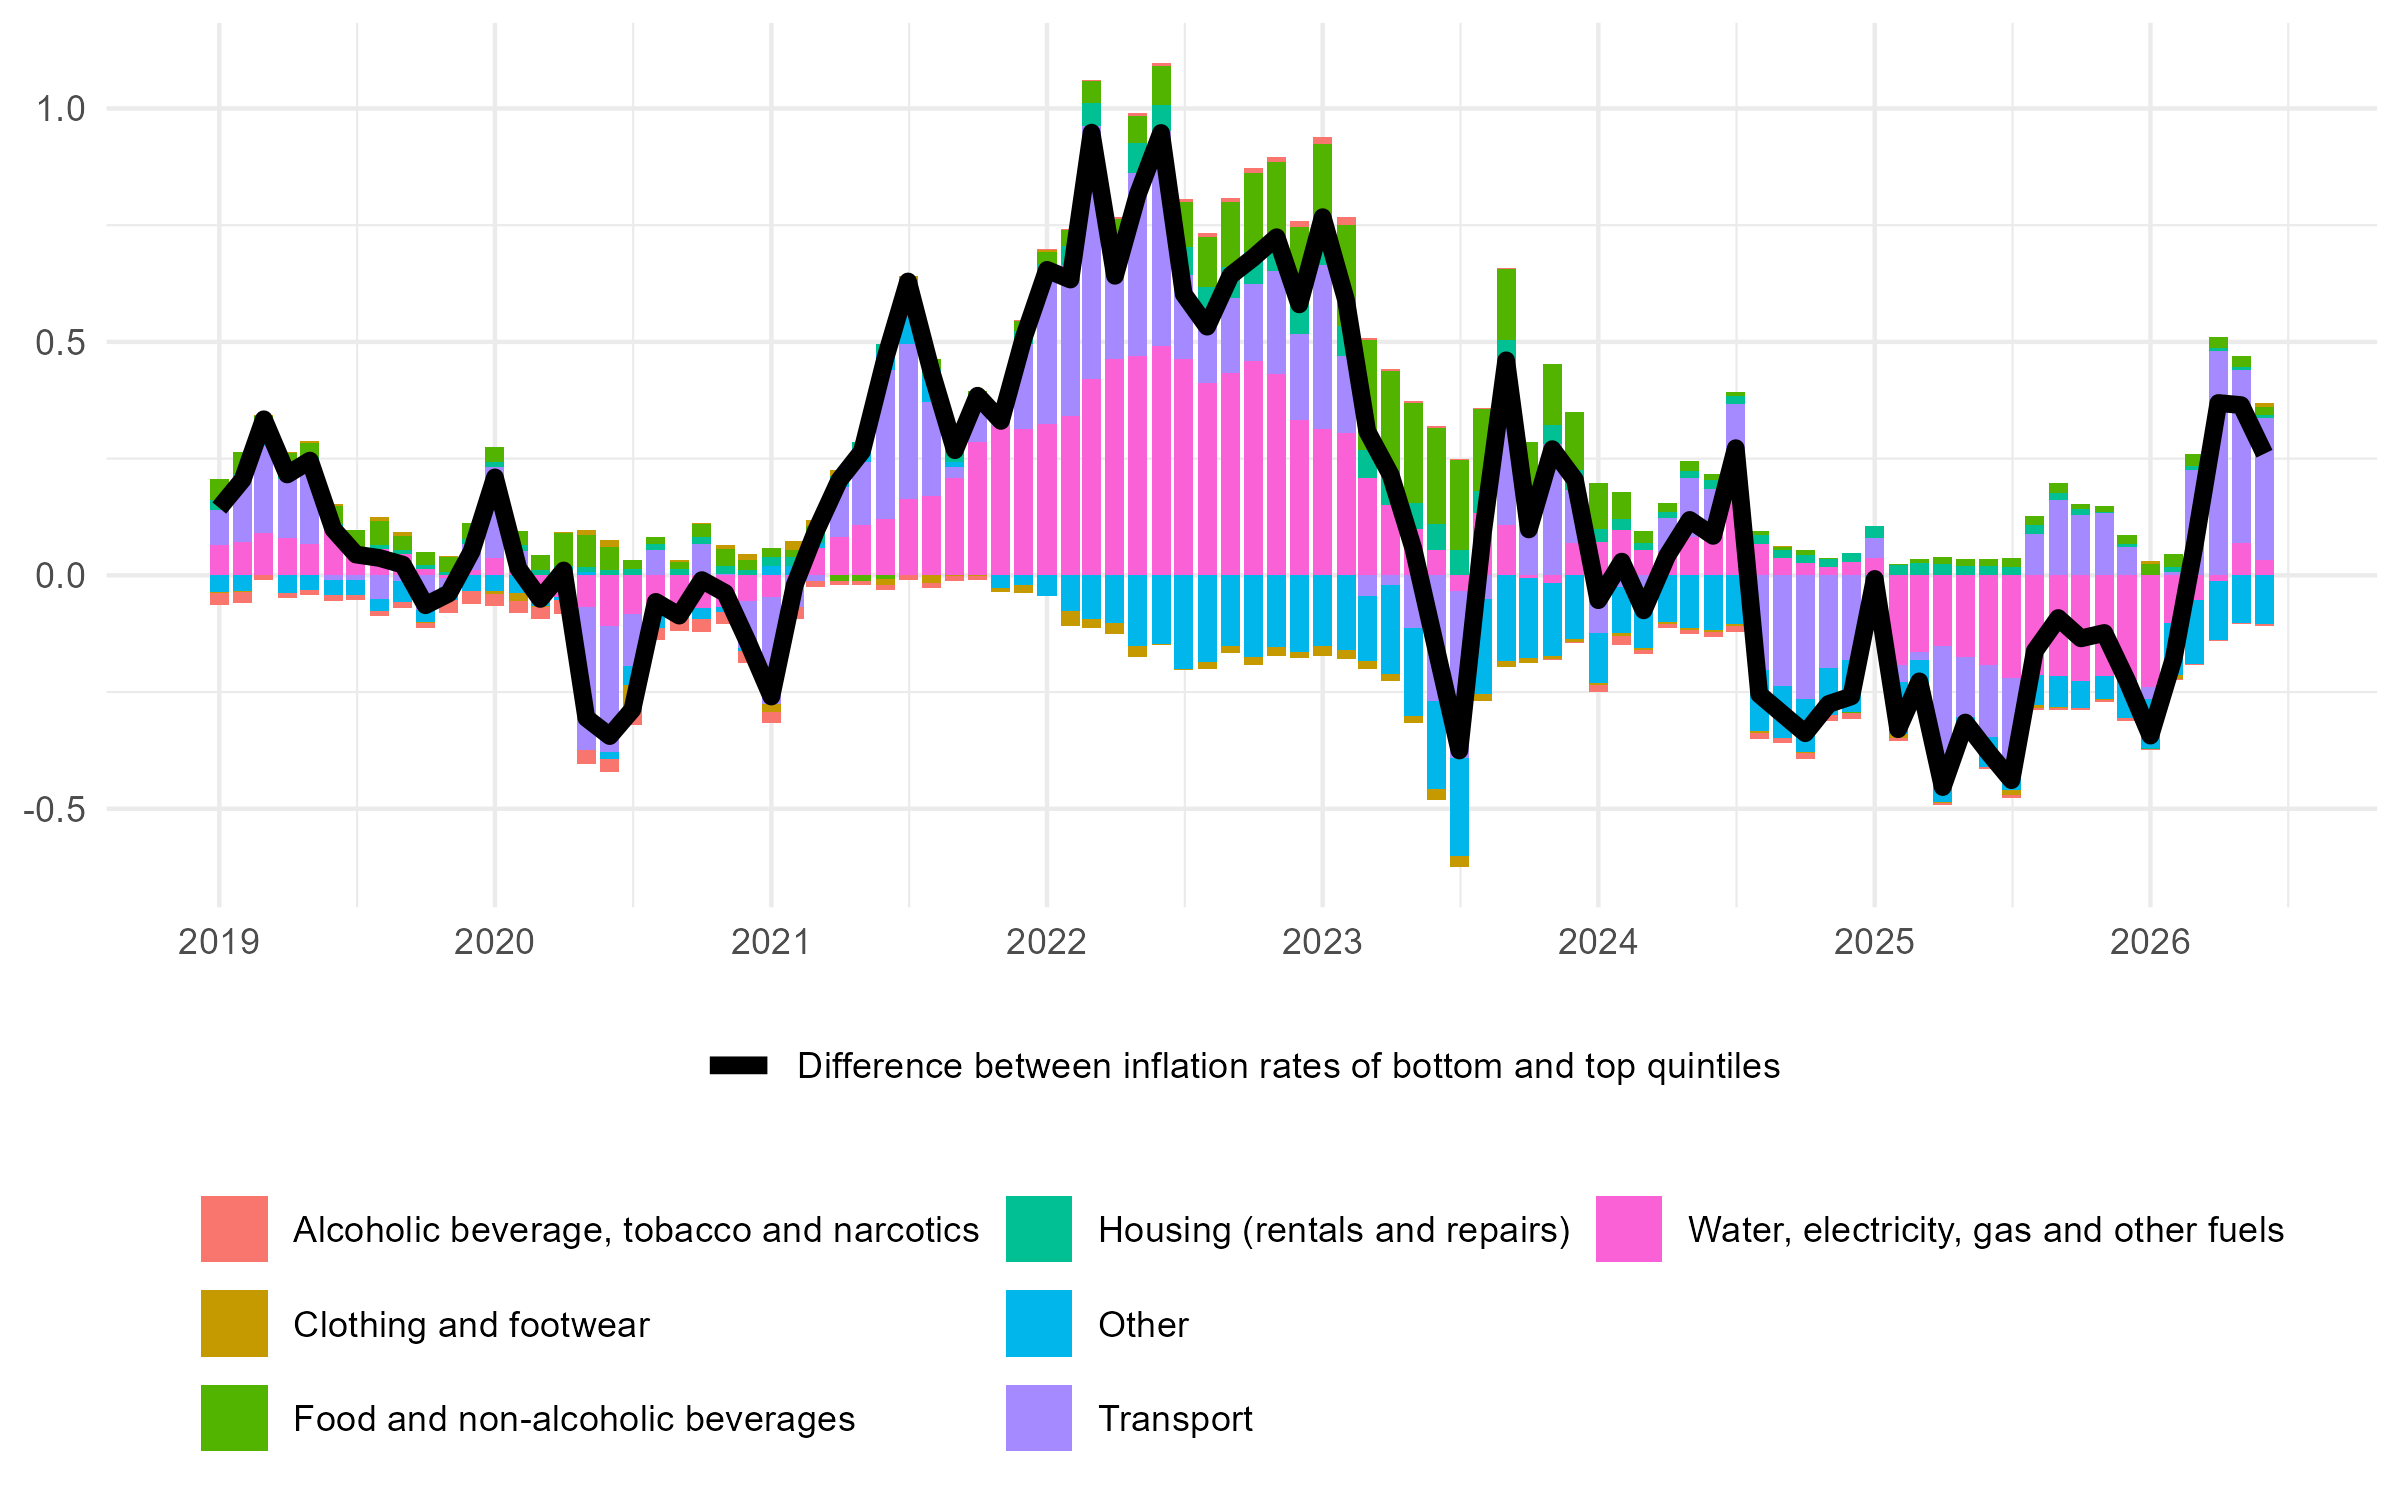
\includegraphics[width=\linewidth,height=0.22\textheight,keepaspectratio]{fig/fig_FR_2019_2026_urban_contribution_gap_level3_rural_paris.png}
\end{subfigure}
\vspace{10pt}
\captionsetup{font=footnotesize, format=hang, singlelinecheck=false, justification=justified}
\caption*{Notes: Bars decompose the monthly inflation gap into broad consumption components; the black line reports the total gap. Positive values indicate higher inflation for the first group named in each panel.\\
Sources: Eurostat HICP; INSEE HBS 2017; authors' calculations.}
\end{figure}
%%%%%%%%%%%%%%%%%%%%%%%%%%%%%%%%%%%%%%%%%%%%%%%%%%%%%%%%%%%%%%
\newpage


%%%%%%%%%%%%%%%%%%%%%%%%%%%%%%%%%%%%%%%%%%%%%%%%%%%%%%%%%%%%%%
\begin{figure}[H]
\centering
\caption{Essential and discretionary expenditures by income quintile, euro area (in \% of total expenditure)}
\label{fig:app-ea-essentials-discretionary}
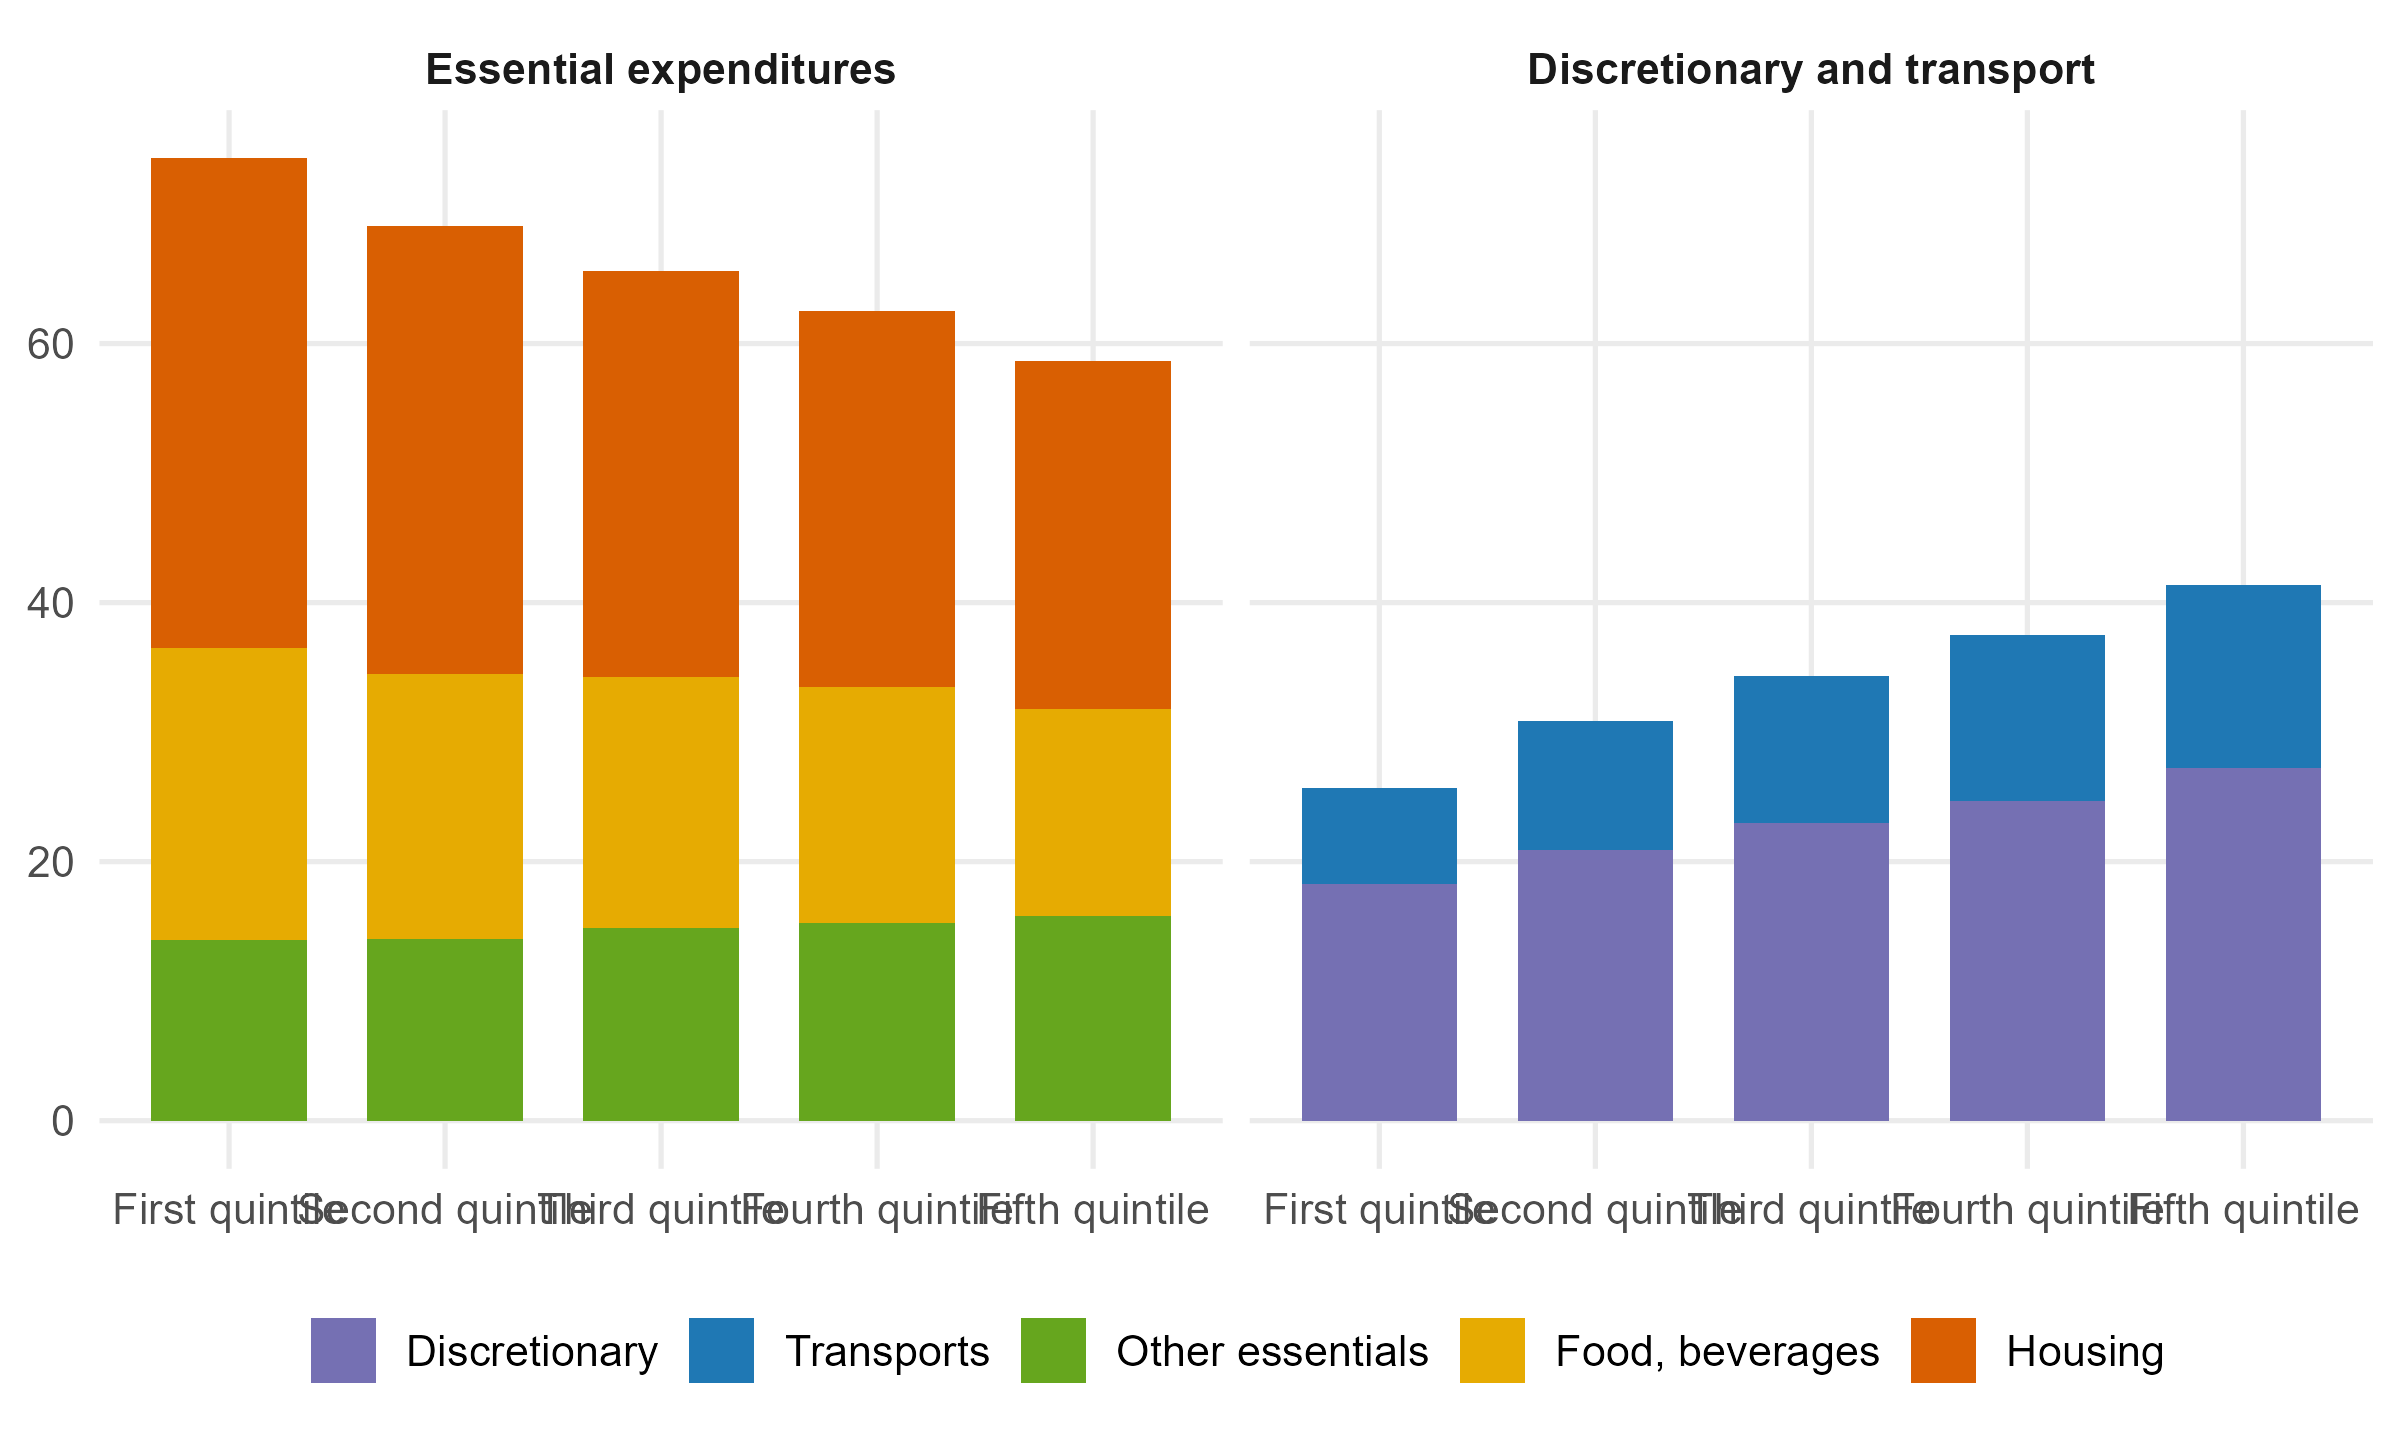
\includegraphics[width=0.88\textwidth,height=0.34\textheight,keepaspectratio]{fig/fig_EA_2015_income_essentials_discretionary_baskets.png}
\vspace{8pt}
\captionsetup{font=footnotesize, format=hang, singlelinecheck=false, justification=justified}
\caption*{Notes: The figure partitions COICOP expenditure shares into essential expenditures and discretionary/transport expenditures. The euro-area aggregate is computed as the unweighted average of available country-level HBS expenditure shares.\\
Source: Eurostat HBS 2015, authors' calculations.}
\end{figure}
%%%%%%%%%%%%%%%%%%%%%%%%%%%%%%%%%%%%%%%%%%%%%%%%%%%%%%%%%%%%%%
\newpage





\section{The Household Budget Survey in Italy}
\label{sec:app-italy-hbs}

While Italy reports HBS data annually on the national statistical office's
website, the most recent Eurostat harmonised and complete HBS entry for Italy is 2005. This
requires a specific treatment for some household-group data. We therefore construct
estimated 2015 and 2020 age and income-quintile baskets.

For age groups, the Italian Istat public-use HBS files for 2015 and 2020 are read directly from the
original files, using the ECOICOP v1 expenditure aggregates available in the
microdata. These direct division-level expenditure variables are used to build
age-group HBS inputs by the age of the household reference person.

For income quintiles, we first use the year in which
income-quintile and expenditure-quintile information can be compared to build a
2005 income/expenditure bridge by COICOP division and quintile, and then apply
this bridge to the target-year Istat HBS baskets by equivalised-expenditure
quintile before renormalising each corrected basket to 100 percent. These bridge-corrected income-quintile baskets are then used as target-year
calibration targets for the latent income-score model, while the household-level
2015 and 2020 Istat HBS public-use files provide the characteristics and
expenditure patterns used to form the target-year groups.

For each household $i$ in target year $y$, let $X_{i,y}$ denote observed
characteristics such as age and education of the reference person,
labour-market status, occupation, housing tenure, housing surface, ownership of
durable goods, internet access, subjective economic resources and situation,
the absolute-poverty indicator, and household consumption level. A latent
socio-economic score is defined as:

\begin{equation}
z_{i,y} = X_{i,y}\beta_y .
\end{equation}

Let $r_{i,y}(\beta_y)$ be the weighted rank of household $i$ in the target-year
distribution of this score. The probability that household $i$ belongs to
latent income group $g \in \{1,\ldots,5\}$ is:

\begin{equation}
p_{i,g,y}(\beta_y)
=
\frac{
\exp\{-\tau [r_{i,y}(\beta_y)-m_g]^2\}
}{
\sum_{h=1}^{5}\exp\{-\tau [r_{i,y}(\beta_y)-m_h]^2\}
},
\end{equation}

where $m_g \in \{0.1,0.3,0.5,0.7,0.9\}$ is the centre of quintile $g$ and
$\tau$ governs the sharpness of the probabilistic assignment. This soft
assignment avoids forcing households close to a quintile boundary into a single
group with probability one.

For COICOP division $j$, the probabilistic expenditure share of group $g$ in
target year $y$ is:

\begin{equation}
\widehat s_{j,g,y}(\beta_y)
=
\frac{
\sum_i w_{i,y} p_{i,g,y}(\beta_y) x_{i,j,y}
}{
\sum_k \sum_i w_{i,y} p_{i,g,y}(\beta_y) x_{i,k,y}
},
\end{equation}

where $w_{i,y}$ is the household survey weight and $x_{i,j,y}$ is household
expenditure on product division $j$. The score parameters are calibrated at the
aggregate level by matching the target-year probabilistic baskets to the
bridge-corrected target-year income-quintile basket:

\begin{equation}
\widehat\beta_y
=
\arg\min_{\beta_y}
\sum_{g=1}^{5}\sum_j
\left[
\widehat s_{j,g,y}(\beta_y)
-
s^{bridge}_{j,g,y}
\right]^2
+ \lambda \|\beta_y\|^2 .
\end{equation}

%This method uses individual and household characteristics in the 2015 and 2020
%Italian HBS files, but the calibration remains aggregate because the target-year
%Italian public-use files do not report observed income quintiles. 
The resulting
groups should therefore be interpreted as latent income groups rather than
directly observed income quintiles. The bridge allows the broad income-group
structure to vary with the target-year expenditure distribution, while retaining the 2005
evidence on how income-quintile and expenditure-quintile baskets differ.

Table~\ref{tab:it-hbs-all-products} reports the aggregate all-products
consumption shares used to document the available Italian HBS inputs. For age
groups, the entries are true survey-weighted shares of annual household
consumption in the target year, computed as group consumption divided by total
household consumption. For income groups, the 2015 and 2020 groups are latent
rather than directly observed survey groups; their aggregate shares are the
bridge-corrected target-year estimates. The resulting Italian distribution is
close to the pattern observed in neighbouring large euro-area countries: the
first quintile accounts for about 8 percent of total consumption, while the fifth
quintile accounts for about 39 percent, compared with roughly 9--10 percent and
33--36 percent in Germany, France and Spain. Table~\ref{tab:it-hbs-latent-income-coefficients}
reports the coefficients of the latent income-score model used to construct
these target-year baskets.

\clearpage

\begin{table}[H]
\small
\setlength{\tabcolsep}{4pt}
\renewcommand{\arraystretch}{0.95}

\caption{\label{tab:it-hbs-all-products}Expenditures by groups (as a share of total expenditures)}
\centering
\begin{tabular}[t]{llll}
\toprule
Dimension & Group & 2015 & 2020\\
\midrule
Age & Less than 30 years & 2.0 & 2.2\\
Age & From 30 to 44 years & 19.7 & 17.9\\
Age & From 45 to 59 years & 34.8 & 34.2\\
Age & 60 years or over & 43.5 & 45.7\\
Income & First quintile & 7.8 & 8.1\\
Income & Second quintile & 12.7 & 12.8\\
Income & Third quintile & 17.2 & 17.0\\
Income & Fourth quintile & 23.3 & 22.8\\
Income & Fifth quintile & 39.0 & 39.3\\
\bottomrule
\end{tabular}
\vspace{-0.6em}
\begin{flushleft}
\footnotesize{Notes. Entries are percent shares of total annual consumption. Age groups follow harmonised Eurostat HBS bands. Income rows for 2015 and 2020 apply the 2005 income/expenditure-quintile bridge to Istat expenditure-quintile baskets. Sources: Istat HBS public-use files, Eurostat HBS, authors' calculations.}
\end{flushleft}
\end{table}


\begin{table}

\caption{\label{tab:it-hbs-latent-income-coefficients}Latent income-score model, Italy}
\centering
\begin{tabular}[t]{lcc}
\toprule
Variable & 2015 & 2020\\
\midrule
Absolute-poverty indicator & 0.142 & 0.001\\
Age of reference person & 0.139 & 0.007\\
Consumption level & 0.157 & -0.017\\
\addlinespace
Economic resources & 0.144 & 0.017\\
Education of reference person & 0.151 & 0.010\\
\addlinespace
Housing surface per person & 0.149 & -0.006\\
Housing tenure & 0.145 & 0.002\\
Labour-market status & 0.137 & -0.000\\
\addlinespace
Occupation & 0.143 & 0.001\\
Subjective economic situation & 0.145 & -0.002\\
\bottomrule
\end{tabular}
\end{table}
\begin{flushleft}
\footnotesize{Notes. The table reports coefficients of the latent socio-economic score used to construct probabilistic income groups in the 2015 and 2020 Istat HBS public-use files. The model excludes household-size, age-squared, rooms-per-person variables and region or macro-region fixed effects. Continuous variables are standardised. The coefficients should be read as score weights used for basket construction rather than causal estimates. Sources: Istat HBS public-use files, Eurostat HBS, authors' calculations.}
\end{flushleft}


\newpage

\section{Weighting}
\label{sec:app-weight-normalization}

We use the RAS (Row and Column Adjustment Scaling) algorithm.
RAS is a bi-proportional matrix scaling method that alternately rescales rows and columns until the required
marginal totals are matched \citep{bacharach1965estimating}. In our setting,
we combine official HICP item weights with the relative HBS
expenditure profile of each household group.

Let $s_{g,y}$ denote the share of group $g$ in total consumption expenditure
used for HICP weight year $y$:
\begin{equation}
s_{g,y}
=
\frac{E^{HBS}_{g,y'}}{E^{HBS}_{\mathrm{all},y'}},
\qquad
\sum_g s_{g,y}=1,
\end{equation}
where $y'$ is the HBS wave matched to HICP weight year $y$. In the
implementation, $s_{g,y}$ is selected from the group consumption-share table
using the most recent HBS wave available at or before $y$; if no prior wave is
available, the earliest available wave is used. These targets are expenditure
shares, not population shares. For Italy, the income targets use the
Istat-based HBS inputs described in Appendix~\ref{sec:app-italy-hbs}.

Let $\mathcal{J}_y$ be the set of matched COICOP categories available in the
HICP weighting structure in year $y$. The RAS seed is
\begin{equation}
Z_{j,g,y}
=
\max\left\{
s_{g,y}\omega^{HICP}_{j,y}c^{HBS}_{j,g,y'},\epsilon
\right\},
\qquad
\epsilon=10^{-12}.
\end{equation}
The small positive floor is a numerical safeguard to keep
the RAS problem strictly non-negative after HICP-HBS matching. The calibrated
aggregate expenditure matrix $M_{j,g,y}$ is required to satisfy the original
HICP item-weight margins:
\begin{equation}
\sum_{j \in \mathcal{J}_y} M_{j,g,y}
=
s_{g,y}\sum_{j \in \mathcal{J}_y}\omega^{HICP}_{j,y}
\quad \text{for all } g,
\qquad
\sum_g M_{j,g,y}
=
\omega^{HICP}_{j,y}
\quad \text{for all } j.
\end{equation}

The RAS algorithm starts from $M^{(0)}_{j,g,y}=Z_{j,g,y}$ and repeats two
scaling steps. At iteration $t$, the row adjustment is
\begin{equation}
\widetilde{M}^{(t)}_{j,g,y}
=
M^{(t-1)}_{j,g,y}
\times
\frac{
s_{g,y}%\sum_{\ell \in \mathcal{J}_y}\omega^{HICP}_{\ell,y}
}{
\sum_{\ell \in \mathcal{J}_y} M^{(t-1)}_{\ell,g,y}
},
\end{equation}
and the column adjustment is
\begin{equation}
M^{(t)}_{j,g,y}
=
\widetilde{M}^{(t)}_{j,g,y}
\times
\frac{
\omega^{HICP}_{j,y}
}{
\sum_h \widetilde{M}^{(t)}_{j,h,y}
}.
\end{equation}
We iterate these two steps by weight year until the maximum absolute
row or column marginal error is below $10^{-10}$, with a maximum of 1,000
iterations.

The final group-specific HICP weights are obtained by dividing the calibrated
aggregate mass by the group expenditure share:
\begin{equation}
\omega_{j,g,y}
=
\frac{M_{j,g,y}}{s_{g,y}}.
\end{equation}
Thus the expenditure-share-weighted average of the group baskets reproduces
the official HICP item weights over the matched product set:
\begin{equation}
\sum_g s_{g,y}\omega_{j,g,y}
=
\omega^{HICP}_{j,y}.
\end{equation}
This preserves the relative information contained in the HBS expenditure
profiles while making the aggregate of the household-group baskets consistent
with the published HICP weighting structure, up to residual differences induced
by product coverage and COICOP matching.

Table~\ref{tab:de-normalization-validation} compares the two weights for
Germany at COICOP level 2 over the period beginning in 2019. The RAS
calibration tracks the published German HICP more closely than the relative-expenditure weighting, whose implicit aggregate weights are equal across groups.%$\omega_{j,y)}*\c_{j,g,y'}$

\begin{table}[H]
\centering
\caption{\label{tab:de-normalization-validation}Germany HICP validation by weighting scheme (differences in pp)}
\small
\begin{tabular}{lrrrrr}
\toprule
Method & Obs. & Mean diff. & Mean abs. diff. & RMSE & Max abs. diff. \\
\midrule
RAS & 88 & -0.059 & 0.093 & 0.118 & 0.259 \\
Relative expenditure & 88 & -0.070 & 0.143 & 0.166 & 0.449 \\
\bottomrule
\end{tabular}
\begin{minipage}{0.86\textwidth}
\footnotesize
Notes: validation statistics compare the recalculated average of German
income-quintile inflation rates with the published all-items HICP inflation
rate. The sample is monthly, from January 2019 to April 2026. All differences
are recalculated minus published inflation and are reported in percentage
points.
\end{minipage}
\end{table}




\clearpage
\begingroup
\setlength{\textfloatsep}{4pt plus 1pt minus 1pt}
\setlength{\floatsep}{4pt plus 1pt minus 1pt}
\setlength{\intextsep}{4pt plus 1pt minus 1pt}
\captionsetup{font=scriptsize,hypcap=false}

\section{Validation Tests}
\label{sec:app-validation-tests}
\enlargethispage{2\baselineskip}

This appendix reports three validation checks for the recalculated French
inflation series: agreement with published HICP, aggregation of quintile
inflation rates, and comparison with official INSEE decile inflation.

\vspace{-0.5em}
\subsection{Internal Consistency}

Figure~\ref{fig:fr-validation-rate} compares level-2 RAS recalculated French
inflation with published all-items HICP. Figure~\ref{fig:fr-validation-level}
compares the total inflation rate with the expenditure-weighted average of
income-quintile inflation rates.

%%%%%%%%%%%%%%%%%%%%%%%%%%%%%%%%%%%%%%%%%%%%%%%%%%%%%%%%%%%%%%
\begin{center}
\centering
\captionof{figure}{Internal consistency: France total inflation and published HICP, level 2 RAS (in \%)}\label{fig:fr-validation-rate}
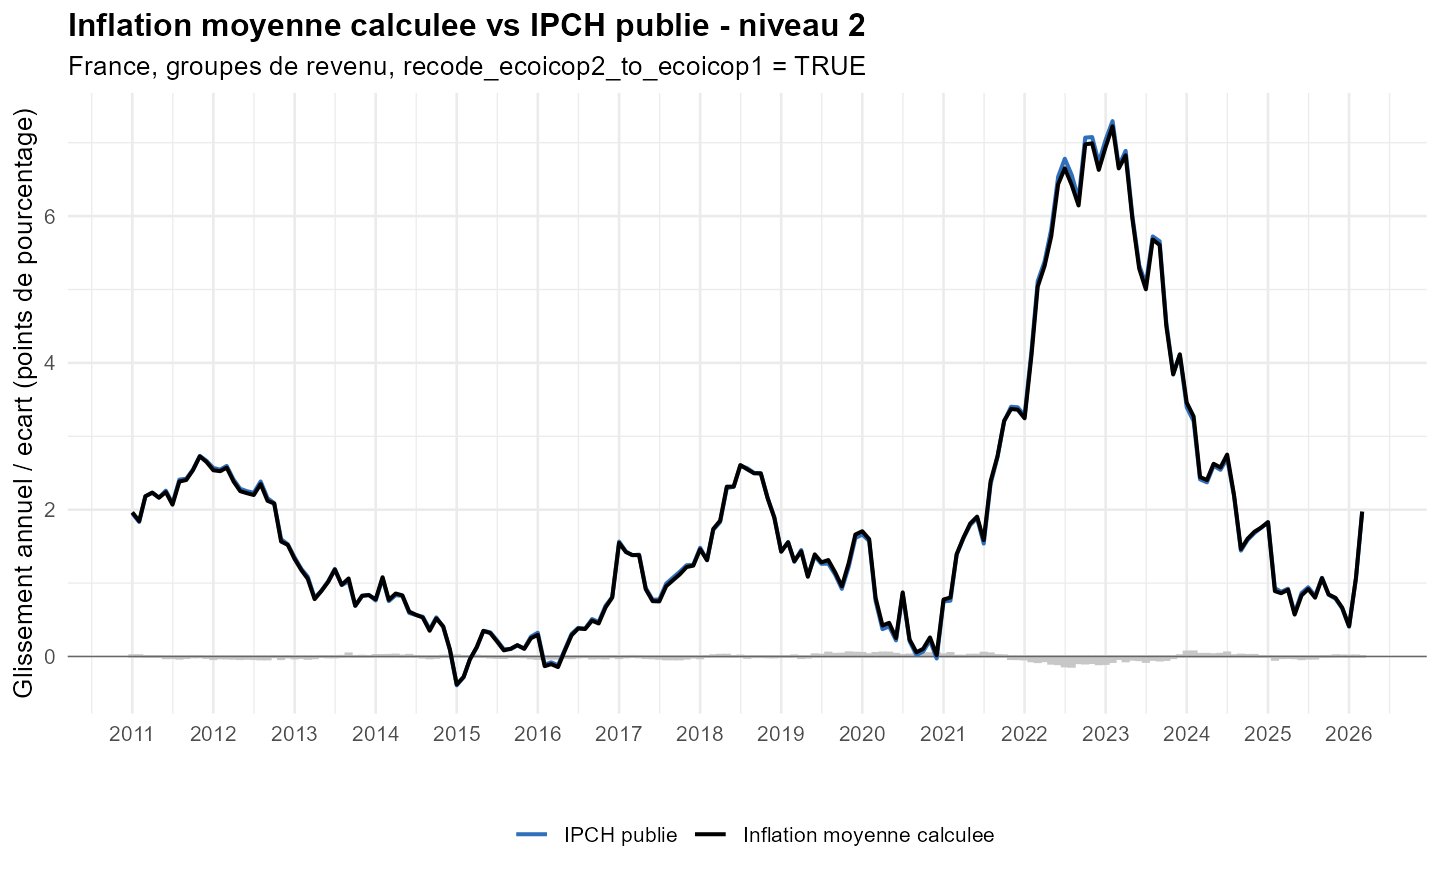
\includegraphics[width=0.95\textwidth,height=0.22\textheight,keepaspectratio]{fig/fig_FR_2010_2026_hicp_inflation_validation_level2_recode_mean_vs_published.png}
\vspace{-2pt}
\captionsetup{font=scriptsize, format=hang, singlelinecheck=false, justification=justified}
\caption*{Note: Blue line: published all-items HICP. Black line: recalculation from 2019 onward. Grey bars: recalculation minus published HICP, in percentage points.\\
Sources: INSEE, Eurostat, authors' calculations.}
\end{center}

%%%%%%%%%%%%%%%%%%%%%%%%%%%%%%%%%%%%%%%%%%%%%%%%%%%%%%%%%%%%%%
\begin{center}
\centering
\captionof{figure}{Internal consistency: France total inflation and weighted average of quintiles, level 2 RAS (in \%)}\label{fig:fr-validation-level}
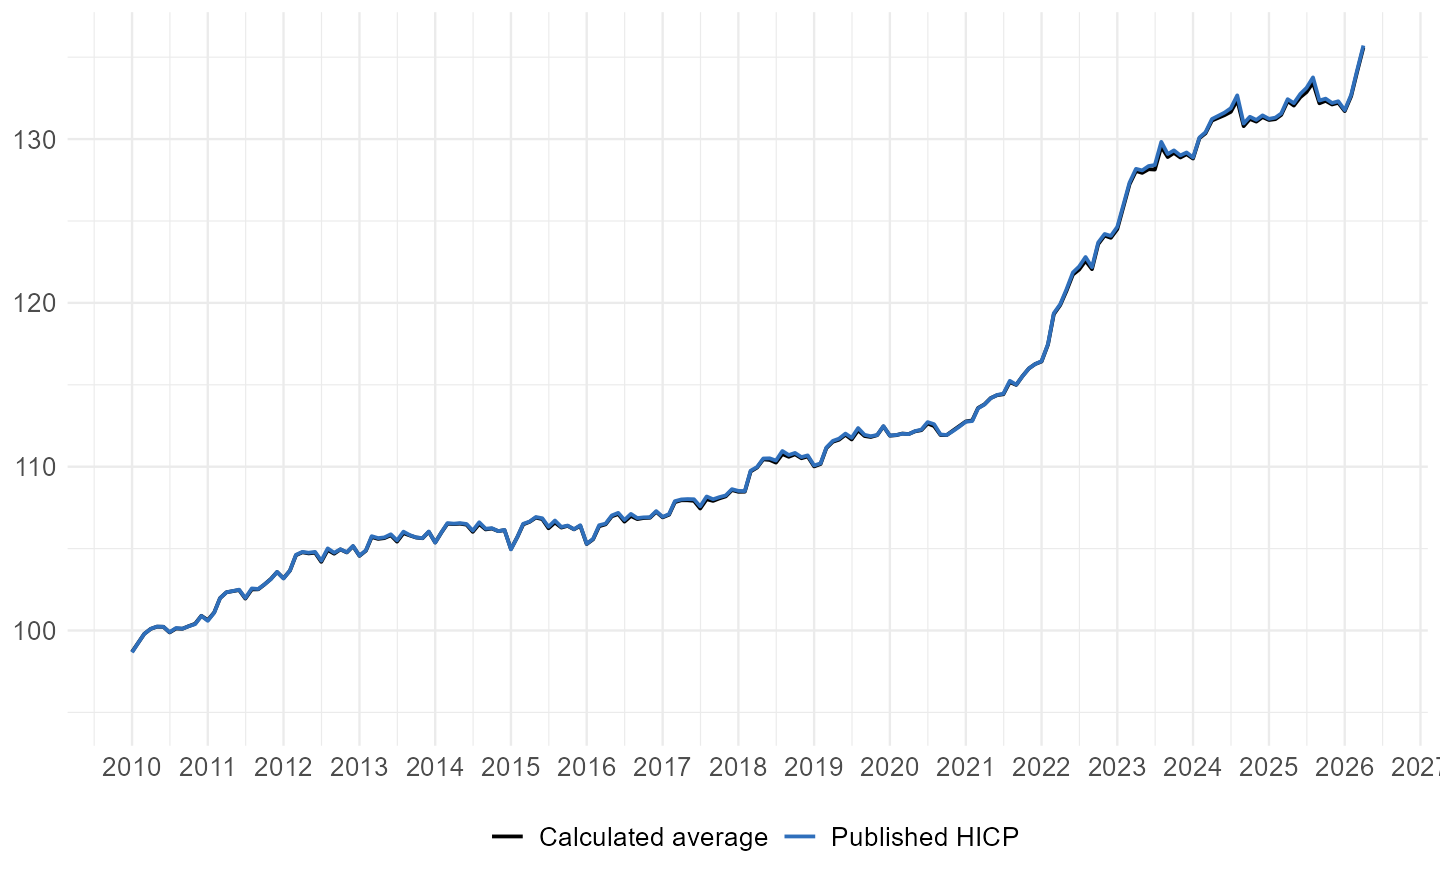
\includegraphics[width=0.95\textwidth,height=0.22\textheight,keepaspectratio]{fig/fig_FR_2010_2026_hicp_validation_level_mean_vs_published.png}
\vspace{-2pt}
\captionsetup{font=scriptsize, format=hang, singlelinecheck=false, justification=justified}
\caption*{Note: Recalculated total inflation and the weighted average of recalculated income-quintile inflation rates. Grey bars: weighted average minus total, in percentage points.\\
Sources: INSEE, Eurostat, authors' calculations.}
\end{center}
%%%%%%%%%%%%%%%%%%%%%%%%%%%%%%%%%%%%%%%%%%%%%%%%%%%%%%%%%%%%%%
\endgroup

\clearpage
\subsection{External Consistency}

Figure~\ref{fig:fr-decile-published-recalculated} compares the
annualized inflation rates computed at COICOP
level 3 with the official INSEE income decile series.

\begin{figure}[H]
\centering
\caption{External consistency: annual inflation by standard-of-living decile, France (in \%)}
\label{fig:fr-decile-published-recalculated}
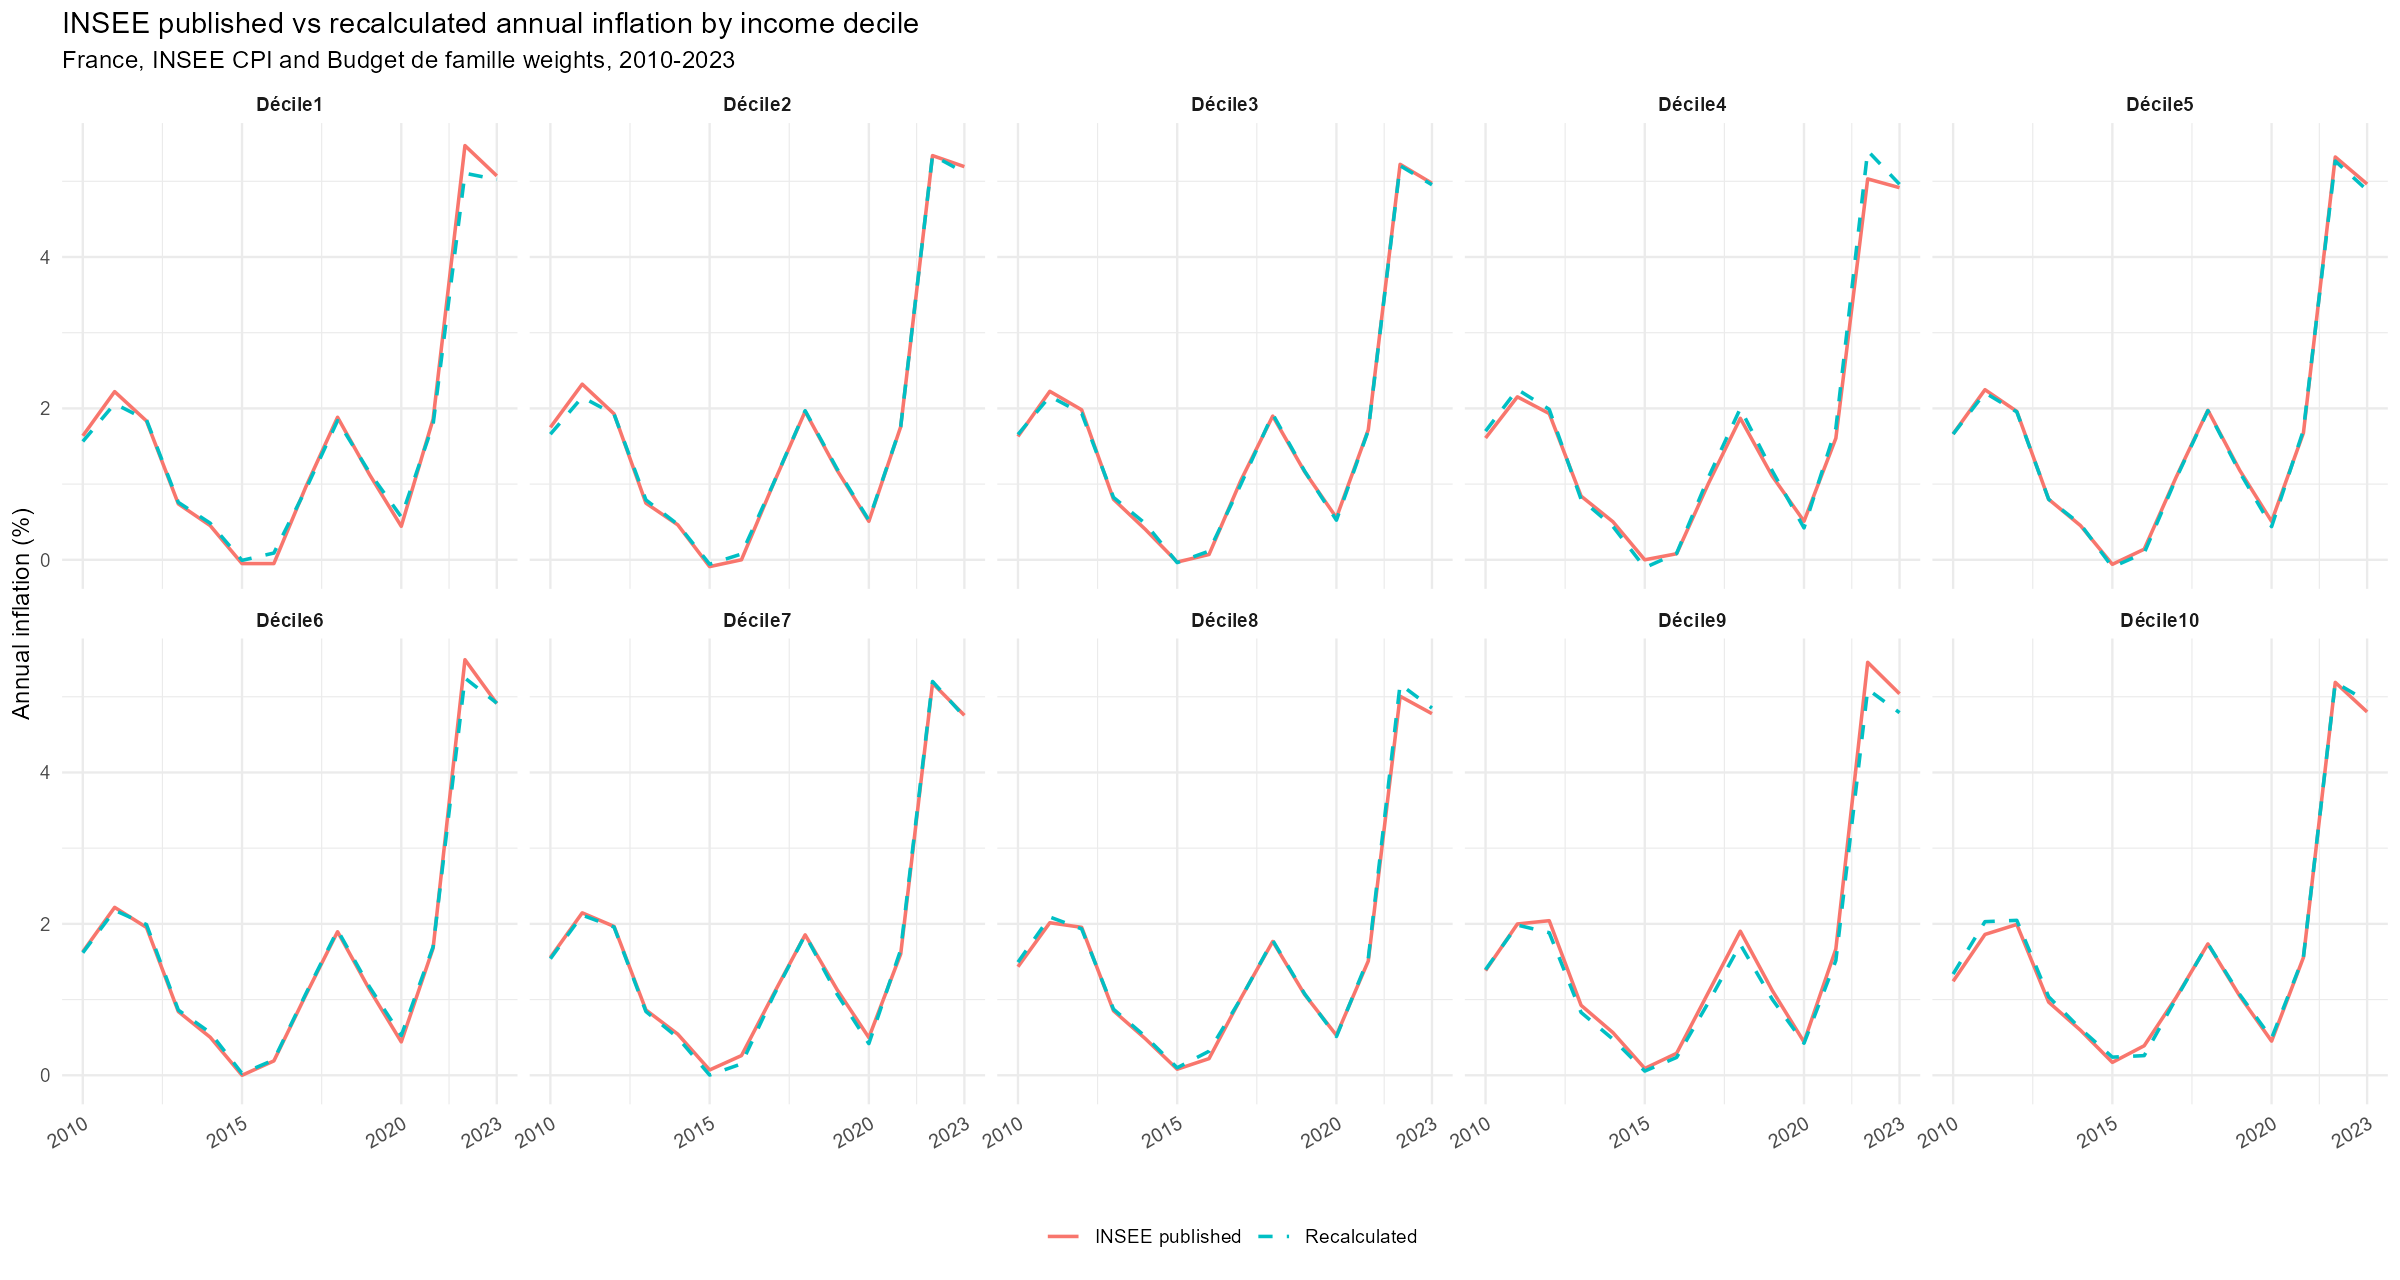
\includegraphics[width=0.95\textwidth,height=0.34\textheight,keepaspectratio]{fig/france-insee-decile-published-vs-recalculated-D1-D10-2010-2023.png}
\captionsetup{font=scriptsize, format=hang, singlelinecheck=false, justification=justified}
\caption*{Note: Official INSEE annual inflation rates by standard-of-living decile are compared with the recalculation at COICOP level 3.\\
Sources: INSEE, Eurostat, authors' calculations.}
\end{figure}

\newpage




% Auto-generated by scripts/07b_build_counterfactuals_appendix.R.
\clearpage
\begin{landscape}
\section{Counterfactuals}
\label{sec:app-counterfactuals}

This appendix reports country-level observed and counterfactual headline inflation series. Each figure aggregates all simulated energy and food price-policy layers available for the country, using the HICP item weights in the country CPI basket.

% Auto-generated from data/counterfactual_measure_assumptions.xlsx (include = TRUE).
\begin{landscape}
\scriptsize
\setlength{\LTleft}{0pt}
\setlength{\LTright}{0pt}
\setlength{\tabcolsep}{2pt}
\renewcommand{\arraystretch}{1.08}
\captionof{table}{Price measures and assumptions included in the national counterfactual simulations}
\label{tab:ea20-price-counterfactual-measures}
\vspace{0.3em}
\begin{longtable}{@{}p{0.62in}p{2.55in}p{2.15in}p{1.30in}p{2.05in}@{}}
\toprule
Country & Included price measure & Rate cut or retained assumption & Start--end dates & Notes \\
\midrule
\endfirsthead
\toprule
Country & Included price measure & Rate cut or retained assumption & Start--end dates & Notes \\
\midrule
\endhead
\midrule
\multicolumn{5}{r}{\emph{Continued on next page}}\\
\endfoot
\bottomrule
\endlastfoot
Austria & Electricity excise reduced from 1.5 to 0.1 ct/kWh & Calibrated no-policy/observed price ratio: 1.05 (+5\%) & 2022-05-01--2024-12-01 &  \\
Austria & Natural-gas excise reduced from 6.6 to 1.196 ct/m3 & Calibrated no-policy/observed price ratio: 1.045 (+4.5\%) & 2022-05-01--2024-12-01 &  \\
Austria & Electricity cost brake: 10 ct/kWh base price, subsidy capped at 30 ct/kWh for 2,900 kWh & Calibrated no-policy/observed price ratio: 1.48 (+48\%) & 2022-12-01--2024-06-01 & Required tariff microdata unavailable. \\
Austria & Electricity cost brake reduced phase: subsidy capped at 15 ct/kWh for 2,900 kWh & Calibrated no-policy/observed price ratio: 1.24 (+24\%) & 2024-07-01--2024-12-01 &  \\
Belgium & Social energy tariff and basic electricity package & Calibrated no-policy/observed price ratio: 1.1 (+10\%) & 2022-03-01--2023-03-01 & Required tariff microdata unavailable. \\
Belgium & Temporary VAT cut on residential electricity from 21\% to 6\% & Calibrated no-policy/observed price ratio: 1.142 (+14.2\%) & 2022-03-01--2022-12-01 &  \\
Belgium & Social energy tariff and basic gas package & Calibrated no-policy/observed price ratio: 1.15 (+15\%) & 2022-04-01--2023-03-01 & Required tariff microdata unavailable. \\
Belgium & Temporary VAT cut on residential natural gas and district heat from 21\% to 6\% & Calibrated no-policy/observed price ratio: 1.142 (+14.2\%) & 2022-04-01--2022-12-01 &  \\
Croatia & Electricity-price mitigation package & Calibrated no-policy/observed price ratio: 1.122 (+12.2\%) & 2022-04-01--2022-09-01 &  \\
Croatia & Gas VAT cut and household price subsidy & Calibrated no-policy/observed price ratio: 1.504 (+50.4\%) & 2022-04-01--2023-03-01 & Specified to avoid double counting. \\
Croatia & VAT cut from 13\% to 5\% on eligible fresh food products & Calibrated no-policy/observed price ratio: 1.04 (+4\%) & 2022-04-01--2023-12-01 & Category coverage is partial. \\
Croatia & District-heating price freeze & Calibrated no-policy/observed price ratio: 1.2 (+20\%) & 2022-10-01--2023-03-01 &  \\
Croatia & Household electricity price cap & Calibrated no-policy/observed price ratio: 1.3 (+30\%) & 2022-10-01--2023-03-01 & Required tariff microdata unavailable. \\
Cyprus & Electricity cost subsidy after VAT reduction & Calibrated no-policy/observed price ratio: 1.12 (+12\%) & 2022-09-01--2023-02-01 & Required tariff microdata unavailable. \\
Estonia & 50\% reimbursement of electricity network fees & Calibrated no-policy/observed price ratio: 1.1 (+10\%) & 2021-10-01--2022-03-01 & Relief applies to one bill component. \\
Estonia & 100\% reimbursement of household gas network fees & Calibrated no-policy/observed price ratio: 1.15 (+15\%) & 2021-12-01--2022-03-01 &  \\
Estonia & 65\% compensation of district-heating increase above October 2021 tariff & Calibrated no-policy/observed price ratio: 1.2 (+20\%) & 2022-02-01--2022-03-01 & Tariffs vary across municipalities. \\
Estonia & Household electricity price compensation & Calibrated no-policy/observed price ratio: 1.2 (+20\%) & 2022-10-01--2023-03-01 & Budget evidence does not identify prices. \\
Estonia & Household natural-gas price compensation & Calibrated no-policy/observed price ratio: 1.2 (+20\%) & 2022-10-01--2023-03-01 &  \\
Finland & Temporary 7.5 percentage-point reduction in the biofuel distribution obligation & Calibrated no-policy/observed price ratio: 1.03 (+3\%) & 2022-05-01--2023-12-01 & Budget evidence does not identify prices. \\
Finland & Temporary electricity VAT reduction from 24\% to 10\% & Calibrated no-policy/observed price ratio: 1.127 (+12.7\%) & 2023-01-01--2023-04-01 &  \\
France & Gas tariff freeze and subsequent gas price cap & Monthly source trajectory; scalar fallback ratio: 1.2 (+20\%) & 2021-11-01--2023-12-01 & Monthly trajectory used; scalar is fallback. \\
France & Regulated electricity tariff cap and TICFE/TCCFE reduction & Monthly source trajectory; scalar fallback ratio: 1.15 (+15\%) & 2022-02-01--2023-12-01 & Monthly trajectory used; scalar is fallback. \\
France & Transport-fuel rebate of 18 then 30 cents per litre & Monthly source trajectory; scalar fallback ratio: 1.12 (+12\%) & 2022-03-01--2022-12-01 & Monthly trajectory used; scalar is fallback. \\
Germany & Early abolition of the EEG electricity levy (3.723 ct/kWh to zero) & Statutory no-policy/observed price ratio: 1.103 (+10.3\%) & 2022-07-01--2022-12-01 & Assumes full pass-through. \\
Germany & Temporary VAT cut on natural gas from 19\% to 7\% & Statutory no-policy/observed price ratio: 1.112 (+11.2\%) & 2022-10-01--2024-03-01 & Assumes full pass-through. \\
Germany & Gas price brake & Calibrated no-policy/observed price ratio: 1.2 (+20\%) & 2023-01-01--2023-12-01 & Required tariff microdata unavailable. \\
Germany & Household electricity price brake: EUR 0.40/kWh on 80\% of reference consumption & Calibrated no-policy/observed price ratio: 1.1 (+10\%) & 2023-01-01--2023-12-01 & Required tariff microdata unavailable. \\
Greece & Electricity consumption subsidy for households & Calibrated no-policy/observed price ratio: 1.35 (+35\%) & 2021-09-01--2023-12-01 & Aggregate proxy; no micro-simulation. \\
Greece & Natural-gas consumption subsidy for households & Calibrated no-policy/observed price ratio: 1.2 (+20\%) & 2021-10-01--2022-12-01 & Eligibility is approximated. \\
Greece & Direct subsidy on automotive diesel & Calibrated no-policy/observed price ratio: 1.08 (+8\%) & 2022-04-01--2022-09-01 & Cash transfers excluded from HICP prices. \\
Ireland & Temporary excise-duty cuts on petrol and diesel & Calibrated no-policy/observed price ratio: 1.1 (+10\%) & 2022-03-01--2023-02-01 &  \\
Ireland & Electricity Costs Emergency Benefit Scheme credits & Calibrated no-policy/observed price ratio: 1.08 (+8\%) & 2022-04-01--2023-03-01 & Credit is per bill, not per kWh. \\
Ireland & Temporary VAT cut on electricity from 13.5\% to 9\% & Calibrated no-policy/observed price ratio: 1.041 (+4.1\%) & 2022-05-01--2023-02-01 &  \\
Ireland & Temporary VAT cut on gas from 13.5\% to 9\% & Calibrated no-policy/observed price ratio: 1.041 (+4.1\%) & 2022-05-01--2023-02-01 &  \\
Ireland & Public Service Obligation levy reduction & Calibrated no-policy/observed price ratio: 1.03 (+3\%) & 2022-10-01--2023-09-01 &  \\
Italy & Electricity general system charges removed & Calibrated no-policy/observed price ratio: 1.09 (+9\%) & 2021-10-01--2023-03-01 & Aggregate proxy; no micro-simulation. \\
Italy & Gas general system charges removed or reduced & Calibrated no-policy/observed price ratio: 1.029 (+2.9\%) & 2021-10-01--2023-12-01 & Specified to avoid double counting. \\
Italy & Strengthened social bonus on electricity bills & Calibrated no-policy/observed price ratio: 1.02 (+2\%) & 2021-10-01--2023-12-01 & Targeted benefit; coverage approximated. \\
Italy & Strengthened social bonus on natural-gas bills & Calibrated no-policy/observed price ratio: 1.02 (+2\%) & 2021-10-01--2023-12-01 & Targeted benefit; coverage approximated. \\
Italy & Temporary 5\% VAT rate on household natural gas & Calibrated no-policy/observed price ratio: 1.122 (+12.2\%) & 2021-10-01--2023-12-01 & Aggregate proxy; no micro-simulation. \\
Italy & Temporary excise-duty cuts on petrol and diesel & Calibrated no-policy/observed price ratio: 1.15 (+15\%) & 2022-03-01--2022-11-01 &  \\
Latvia & Removal of OIK and electricity network charges & Calibrated no-policy/observed price ratio: 1.62 (+62\%) & 2022-01-01--2022-04-01 & Aggregate proxy; no micro-simulation. \\
Latvia & Natural-gas heating compensation of EUR 30/MWh & Calibrated no-policy/observed price ratio: 1.2 (+20\%) & 2022-07-01--2023-04-01 & Eligibility is approximated. \\
Latvia & Compensation of 50\% of district-heating tariff above EUR 68/MWh & Calibrated no-policy/observed price ratio: 1.2 (+20\%) & 2022-10-01--2023-04-01 & Tariffs vary across municipalities. \\
Lithuania & Compensation of household electricity prices & Calibrated no-policy/observed price ratio: 1.25 (+25\%) & 2022-07-01--2023-06-01 & Budget evidence does not identify prices. \\
Lithuania & Partial subsidy on household natural-gas prices & Calibrated no-policy/observed price ratio: 1.3 (+30\%) & 2022-07-01--2023-06-01 & Universal household coverage. \\
Luxembourg & Energiedësch electricity-price stabilisation & Calibrated no-policy/observed price ratio: 1.03 (+3\%) & 2022-02-01--2022-12-01 & Required tariff microdata unavailable. \\
Luxembourg & Energiedësch gas-network-fee subsidy & Calibrated no-policy/observed price ratio: 1.05 (+5\%) & 2022-02-01--2022-09-01 &  \\
Luxembourg & Temporary reduction of 7.5 euro cents per litre of motor fuel & Calibrated no-policy/observed price ratio: 1.045 (+4.5\%) & 2022-04-01--2022-08-01 & Aggregate proxy; no micro-simulation. \\
Luxembourg & Natural-gas increase limited to 15\% and state coverage of network costs & Calibrated no-policy/observed price ratio: 1.15 (+15\%) & 2022-10-01--2024-12-01 & Required tariff microdata unavailable. \\
Luxembourg & Residential electricity-price stabilisation at the 2022 level & Calibrated no-policy/observed price ratio: 1.15 (+15\%) & 2023-01-01--2024-12-01 & Required tariff microdata unavailable. \\
Malta & Government subsidy keeping household electricity tariffs stable & Calibrated no-policy/observed price ratio: 1.3 (+30\%) & 2022-01-01--2023-12-01 & Budget evidence does not identify prices. \\
Malta & Government subsidy stabilising petrol and diesel retail prices & Calibrated no-policy/observed price ratio: 1.15 (+15\%) & 2022-01-01--2023-12-01 & Aggregate proxy; no micro-simulation. \\
Netherlands & Temporary 21\% cut in petrol and diesel excise duties & Calibrated no-policy/observed price ratio: 1.08 (+8\%) & 2022-04-01--2022-12-01 &  \\
Netherlands & Temporary VAT cut on energy from 21\% to 9\% - electricity & Calibrated no-policy/observed price ratio: 1.11 (+11\%) & 2022-07-01--2022-12-01 &  \\
Netherlands & Temporary VAT cut on energy from 21\% to 9\% - gas & Calibrated no-policy/observed price ratio: 1.11 (+11\%) & 2022-07-01--2022-12-01 &  \\
Netherlands & Electricity price cap EUR 0.40 per kWh up to 2900 kWh & Calibrated no-policy/observed price ratio: 1.25 (+25\%) & 2023-01-01--2023-12-01 & Required tariff microdata unavailable. \\
Netherlands & Gas price cap EUR 1.45 per m3 up to 1200 m3 & Calibrated no-policy/observed price ratio: 1.35 (+35\%) & 2023-01-01--2023-12-01 & Required tariff microdata unavailable. \\
Portugal & ISP and carbon-tax reductions on petrol and diesel & Calibrated no-policy/observed price ratio: 1.1 (+10\%) & 2022-05-01--2023-12-01 &  \\
Portugal & Electricity VAT reduction from 13\% to 6\% & Calibrated no-policy/observed price ratio: 1.066 (+6.6\%) & 2022-10-01--2023-12-01 &  \\
Portugal & Bread and cereals zero-VAT basket & Statutory no-policy/observed price ratio: 1.06 (+6\%) & 2023-04-01--2023-12-01 &  \\
Portugal & Fish zero-VAT basket & Statutory no-policy/observed price ratio: 1.06 (+6\%) & 2023-04-01--2023-12-01 &  \\
Portugal & Fruit zero-VAT basket & Statutory no-policy/observed price ratio: 1.06 (+6\%) & 2023-04-01--2023-12-01 &  \\
Portugal & Meat zero-VAT basket & Statutory no-policy/observed price ratio: 1.06 (+6\%) & 2023-04-01--2023-12-01 &  \\
Portugal & Milk cheese and eggs zero-VAT basket & Statutory no-policy/observed price ratio: 1.06 (+6\%) & 2023-04-01--2023-12-01 &  \\
Portugal & Oils and fats VAT measures & Statutory no-policy/observed price ratio: 1.117 (+11.7\%) & 2023-04-01--2026-04-01 & Rates vary across statutory subperiods. \\
Portugal & Plant-based drinks VAT measure & Statutory no-policy/observed price ratio: 1.06 (+6\%) & 2023-04-01--2023-12-01 &  \\
Portugal & Vegetables zero-VAT basket & Statutory no-policy/observed price ratio: 1.06 (+6\%) & 2023-04-01--2023-12-01 &  \\
Slovakia & Flat household electricity commodity, distribution and system charges & Calibrated no-policy/observed price ratio: 1.3 (+30\%) & 2023-01-01--2023-12-01 &  \\
Slovakia & Household heat price cap & Calibrated no-policy/observed price ratio: 1.25 (+25\%) & 2023-01-01--2023-12-01 & Required tariff microdata unavailable. \\
Slovakia & Household natural-gas price cap & Calibrated no-policy/observed price ratio: 1.5 (+50\%) & 2023-01-01--2023-12-01 & Budget evidence does not identify prices. \\
Slovenia & Temporary exemption from electricity network charges & Calibrated no-policy/observed price ratio: 1.1 (+10\%) & 2022-03-01--2022-04-01 & Relief applies to one bill component. \\
Slovenia & Temporary exemption from natural-gas network charges & Calibrated no-policy/observed price ratio: 1.08 (+8\%) & 2022-03-01--2022-04-01 & Relief applies to one bill component. \\
Slovenia & Temporary regulated petrol and diesel retail prices & Calibrated no-policy/observed price ratio: 1.1 (+10\%) & 2022-03-01--2022-08-01 &  \\
Slovenia & Household electricity price cap & Calibrated no-policy/observed price ratio: 1.15 (+15\%) & 2022-09-01--2023-08-01 & Required tariff microdata unavailable. \\
Slovenia & Household natural-gas price cap & Calibrated no-policy/observed price ratio: 1.18 (+18\%) & 2022-09-01--2023-08-01 & Required tariff microdata unavailable. \\
Slovenia & District-heating price cap & Calibrated no-policy/observed price ratio: 1.12 (+12\%) & 2023-01-01--2023-04-01 & Required tariff microdata unavailable. \\
Spain & Electricity VAT reduced from 21\% to 10\% & Calibrated no-policy/observed price ratio: 1.1 (+10\%) & 2021-06-01--2022-06-01 & Eligibility is approximated. \\
Spain & Electricity excise duty reduced from 5.11\% to 0.5\% & Calibrated no-policy/observed price ratio: 1.046 (+4.6\%) & 2021-09-01--2023-12-01 &  \\
Spain & EUR 0.20 per litre petrol and diesel discount & Calibrated no-policy/observed price ratio: 1.11 (+11\%) & 2022-04-01--2022-12-01 &  \\
Spain & Iberian mechanism limiting gas input costs in electricity generation & Calibrated no-policy/observed price ratio: 1.2 (+20\%) & 2022-05-01--2023-12-01 & Aggregate proxy; no micro-simulation. \\
Spain & Electricity VAT reduced from 21\% to 5\% & Calibrated no-policy/observed price ratio: 1.152 (+15.2\%) & 2022-07-01--2023-12-01 & Aggregate proxy; no micro-simulation. \\
Spain & Natural-gas VAT reduced from 21\% to 5\% & Calibrated no-policy/observed price ratio: 1.152 (+15.2\%) & 2022-10-01--2023-12-01 &  \\
Spain & Bread and bread flour VAT reduction & Statutory no-policy/observed price ratio: 1.04 (+4\%) & 2023-01-01--2024-12-01 & Rates vary across statutory subperiods. \\
Spain & Fresh fruit VAT reduction & Statutory no-policy/observed price ratio: 1.04 (+4\%) & 2023-01-01--2024-12-01 & Rates vary across statutory subperiods. \\
Spain & Fresh vegetables and pulses VAT reduction & Statutory no-policy/observed price ratio: 1.04 (+4\%) & 2023-01-01--2024-12-01 & Rates vary across statutory subperiods. \\
Spain & Milk cheese and eggs VAT reduction & Statutory no-policy/observed price ratio: 1.04 (+4\%) & 2023-01-01--2024-12-01 & Rates vary across statutory subperiods. \\
Spain & Olive oil and other edible oils VAT reduction & Statutory no-policy/observed price ratio: 1.074 (+7.4\%) & 2023-01-01--2026-04-01 & Rates vary across statutory subperiods. \\
\end{longtable}
\par\vspace{0.35em}\footnotesize\noindent \emph{Notes:} Each row corresponds to a unique measure marked \texttt{include = TRUE} in \texttt{counterfactual\_measure\_assumptions.xlsx}. Ratios report the counterfactual no-policy price divided by the observed policy-inclusive price. \emph{Statutory} denotes a tax or charge inversion based on the legislated rate; \emph{Calibrated} denotes an aggregate-equivalent price assumption. Where a monthly source trajectory is available, it is used in preference to the displayed scalar fallback. \emph{Sources:} Authors' assumptions workbook and calculations.
\end{landscape}

\end{landscape}
\clearpage

\subsection{Belgium}
\begin{figure}[H]
\centering
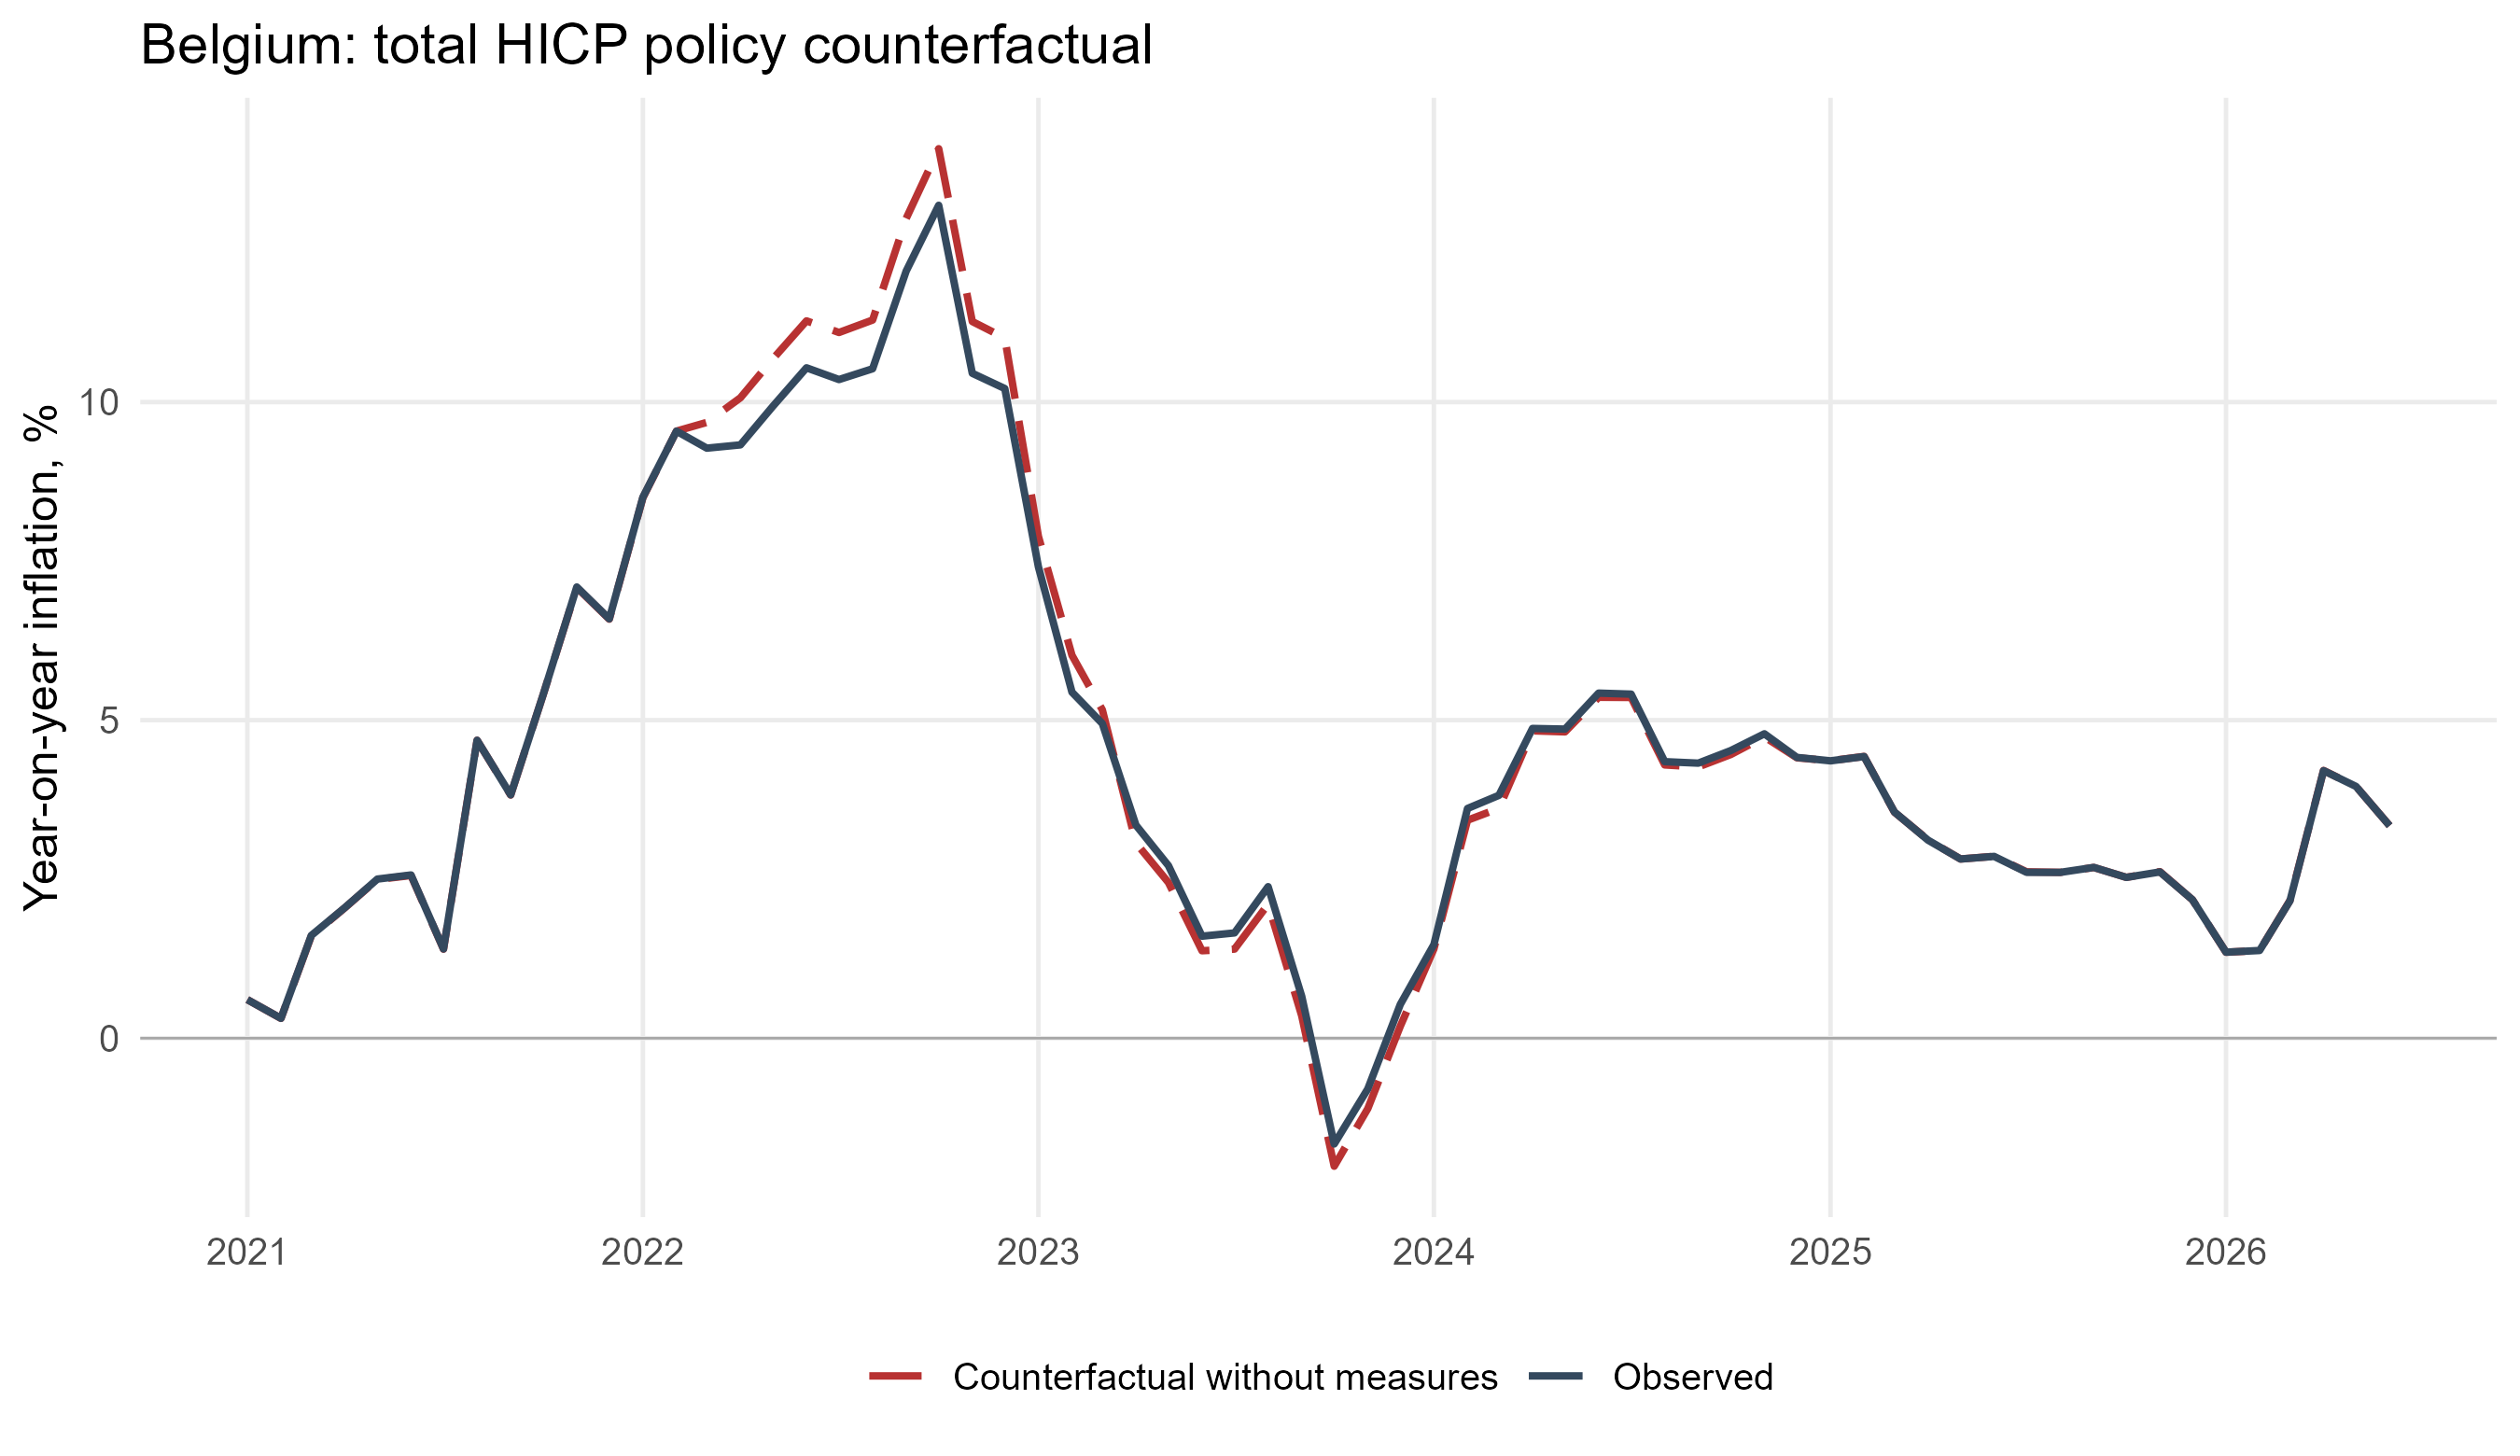
\includegraphics[width=0.86\textwidth,height=0.38\textheight,keepaspectratio]{fig/policy_total_cpi_counterfactual_inflation_BE_belgium.png}
\caption{Belgium: observed and counterfactual inflation}
\end{figure}

\subsection{Cyprus}
\begin{figure}[H]
\centering
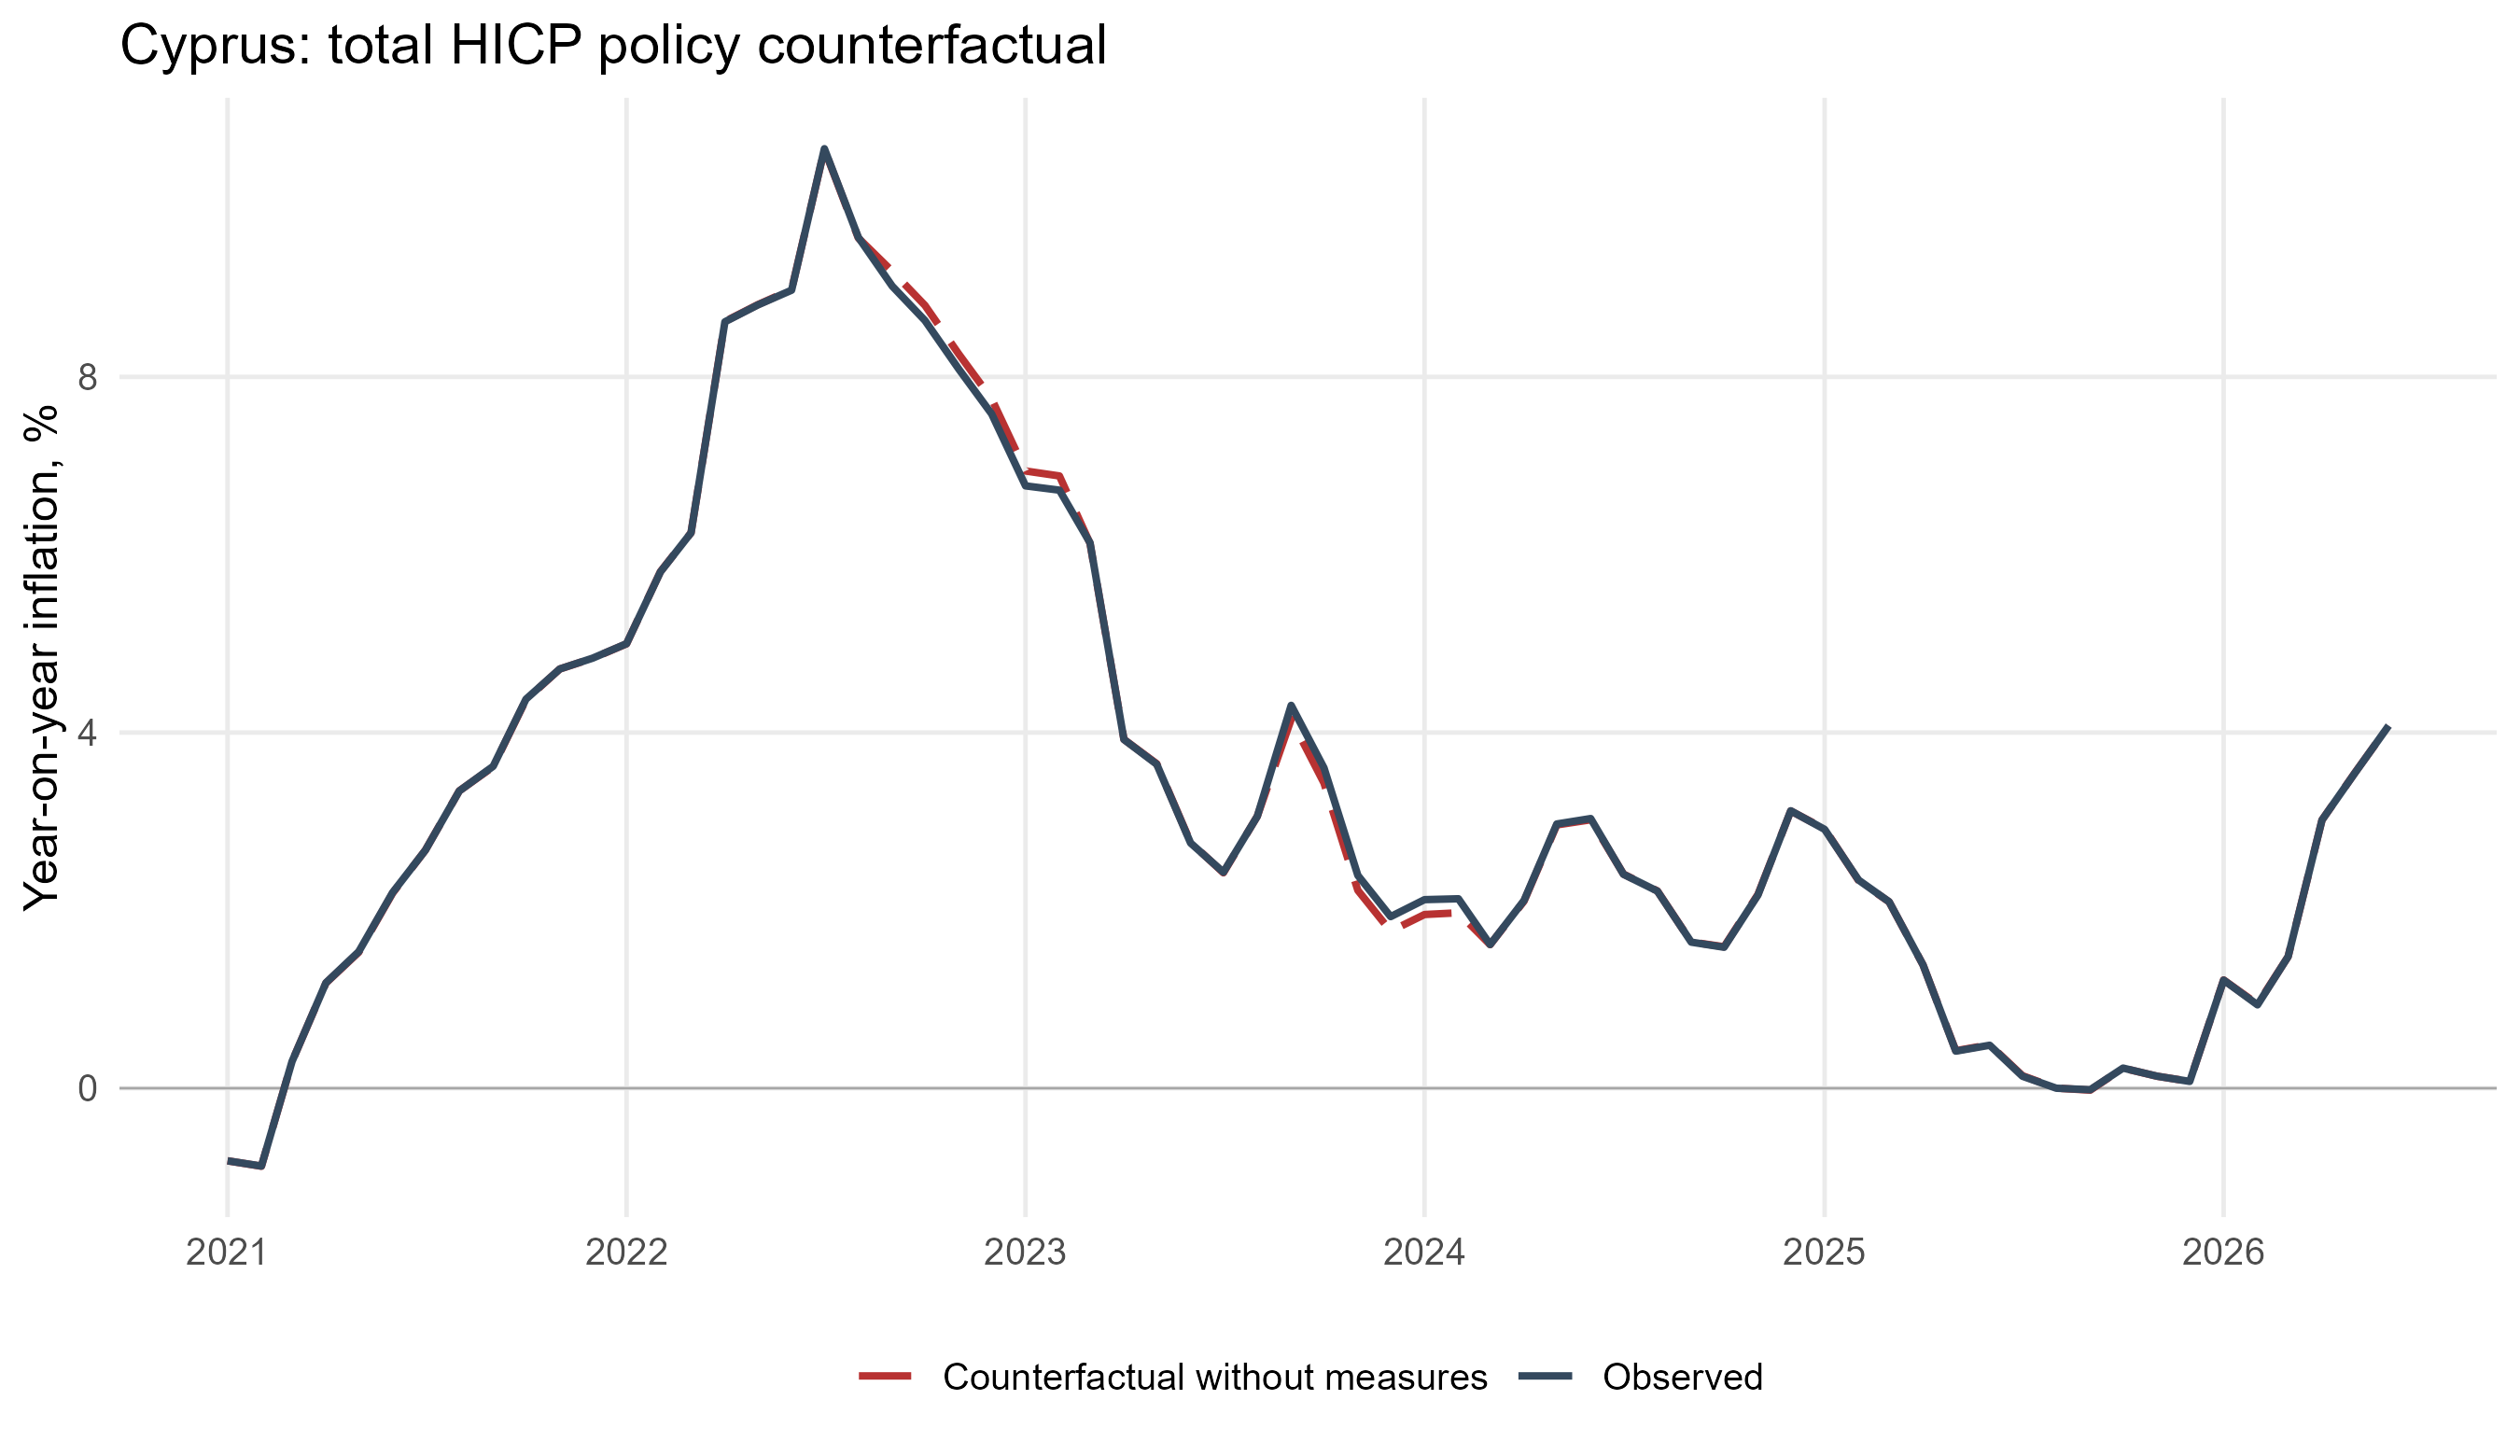
\includegraphics[width=0.86\textwidth,height=0.38\textheight,keepaspectratio]{fig/policy_total_cpi_counterfactual_inflation_CY_cyprus.png}
\caption{Cyprus: observed and counterfactual inflation}
\end{figure}

\subsection{Germany}
\begin{figure}[H]
\centering
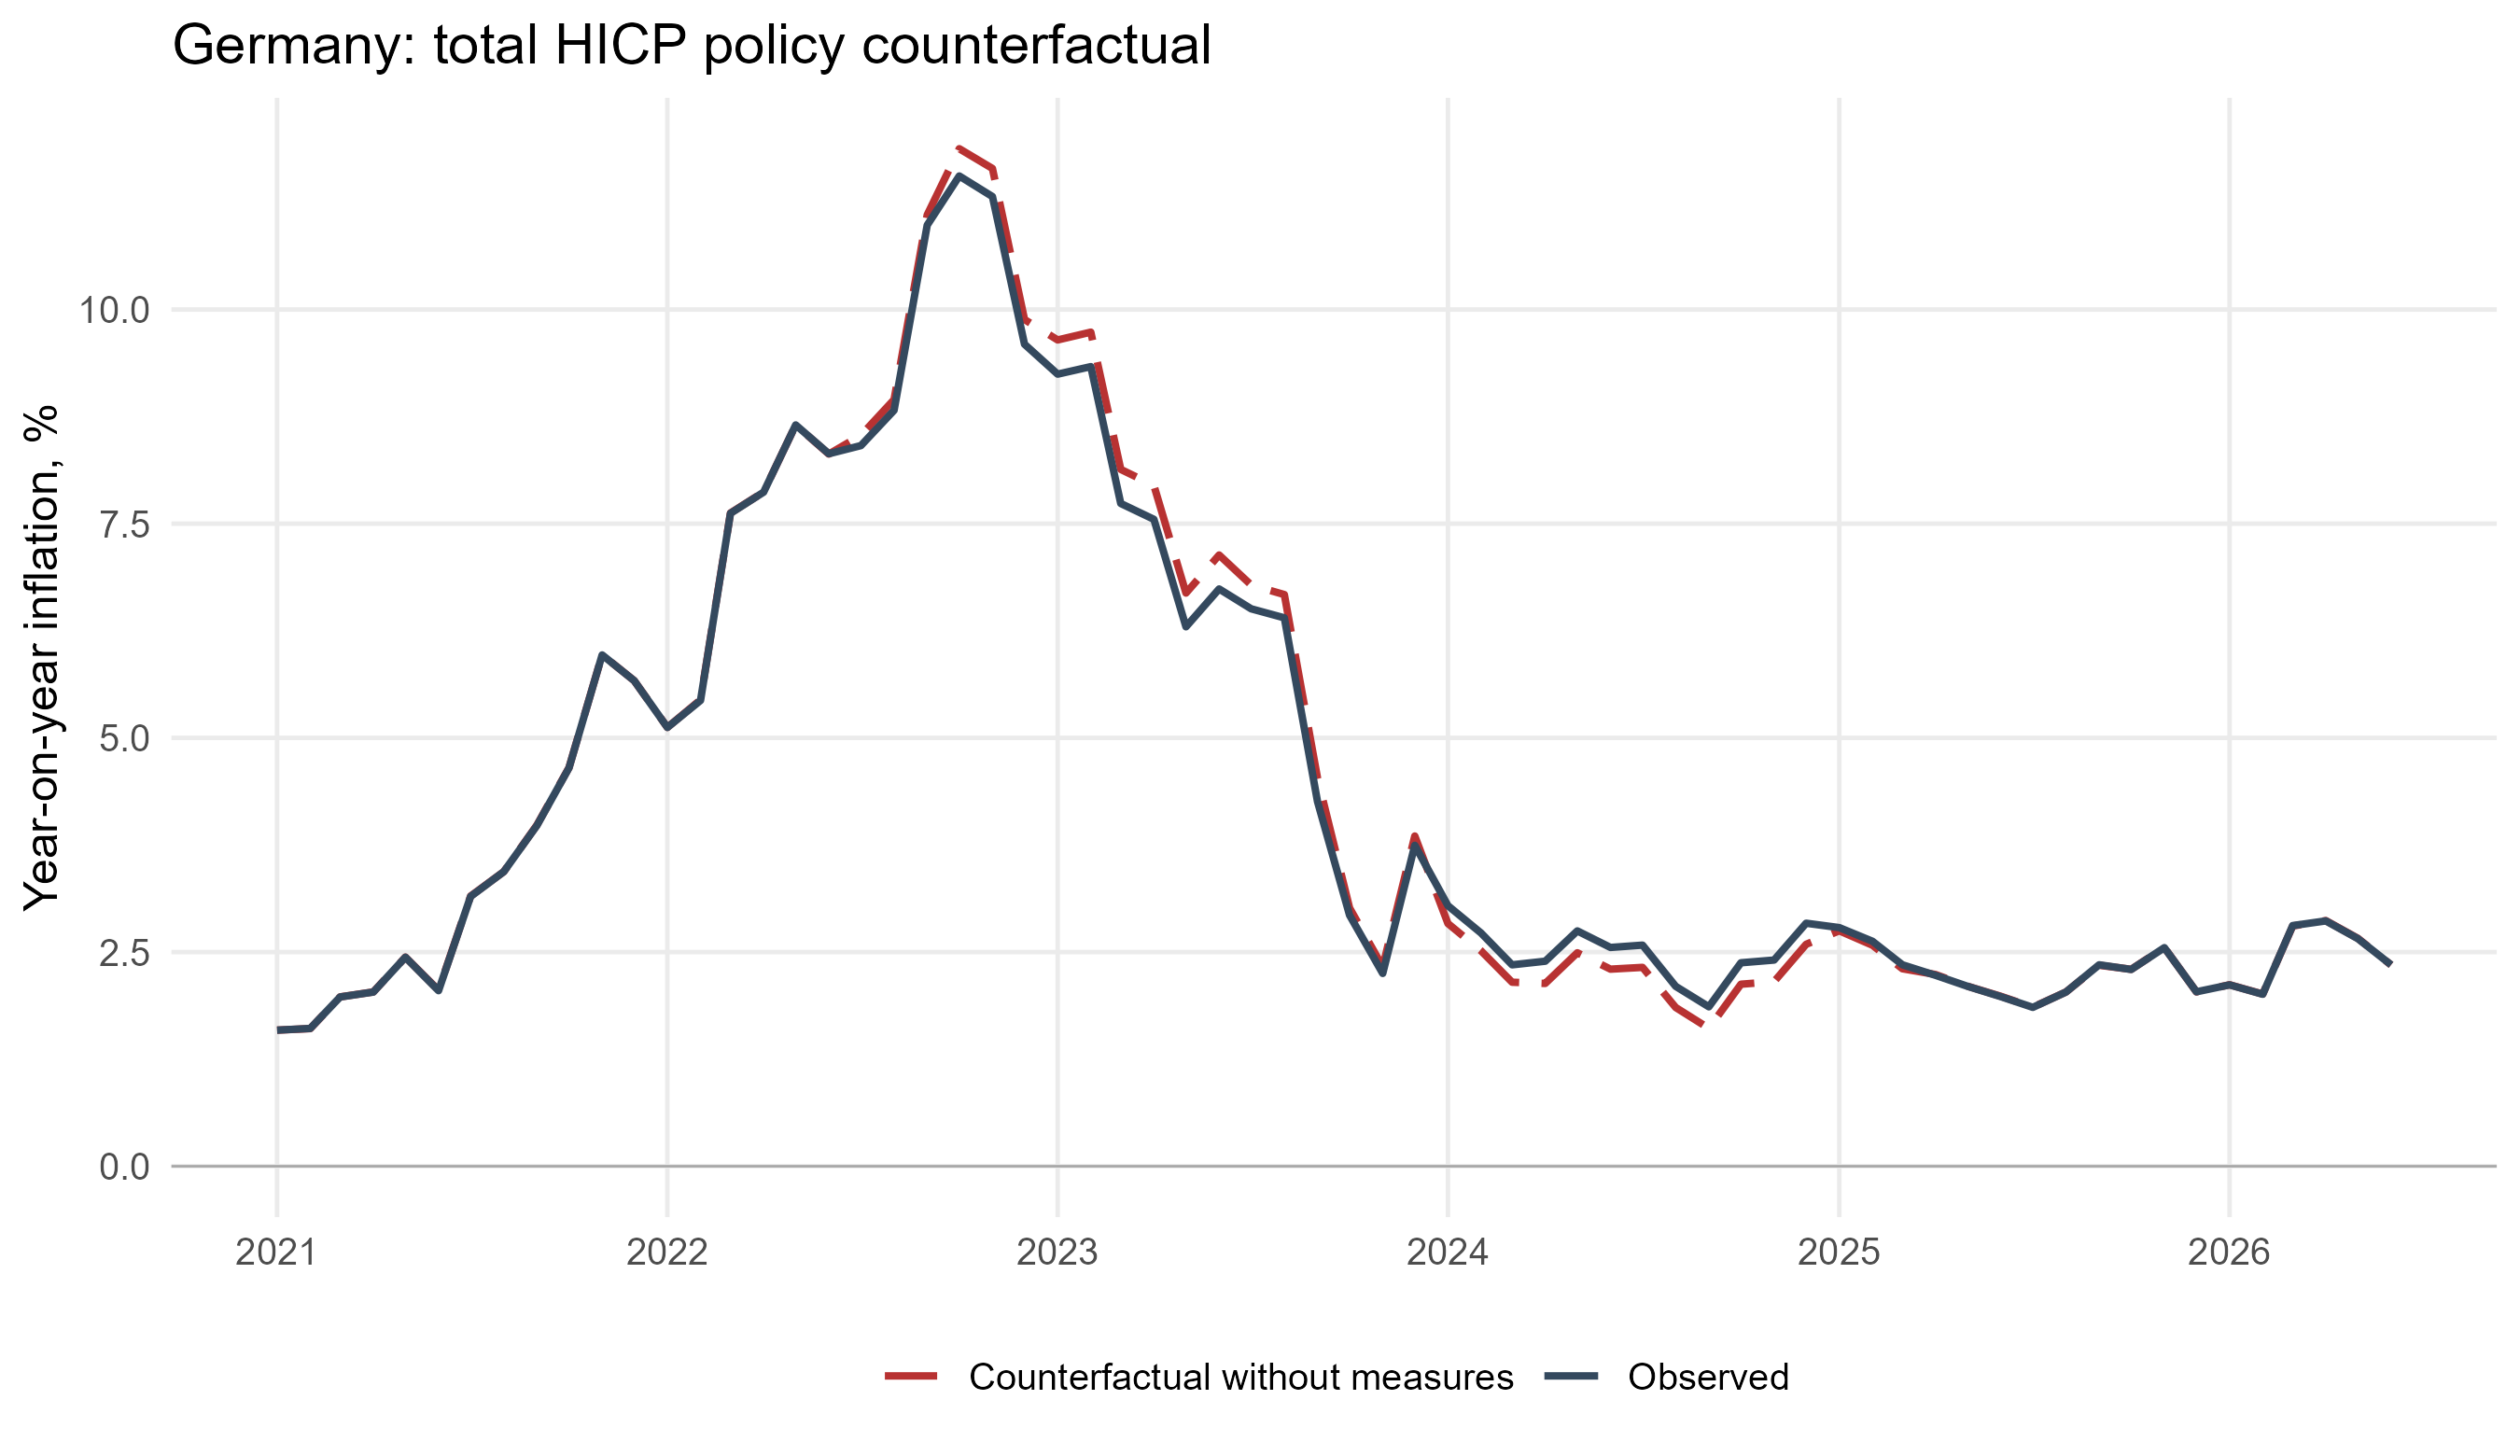
\includegraphics[width=0.86\textwidth,height=0.38\textheight,keepaspectratio]{fig/policy_total_cpi_counterfactual_inflation_DE_germany.png}
\caption{Germany: observed and counterfactual inflation}
\end{figure}

\subsection{Greece}
\begin{figure}[H]
\centering
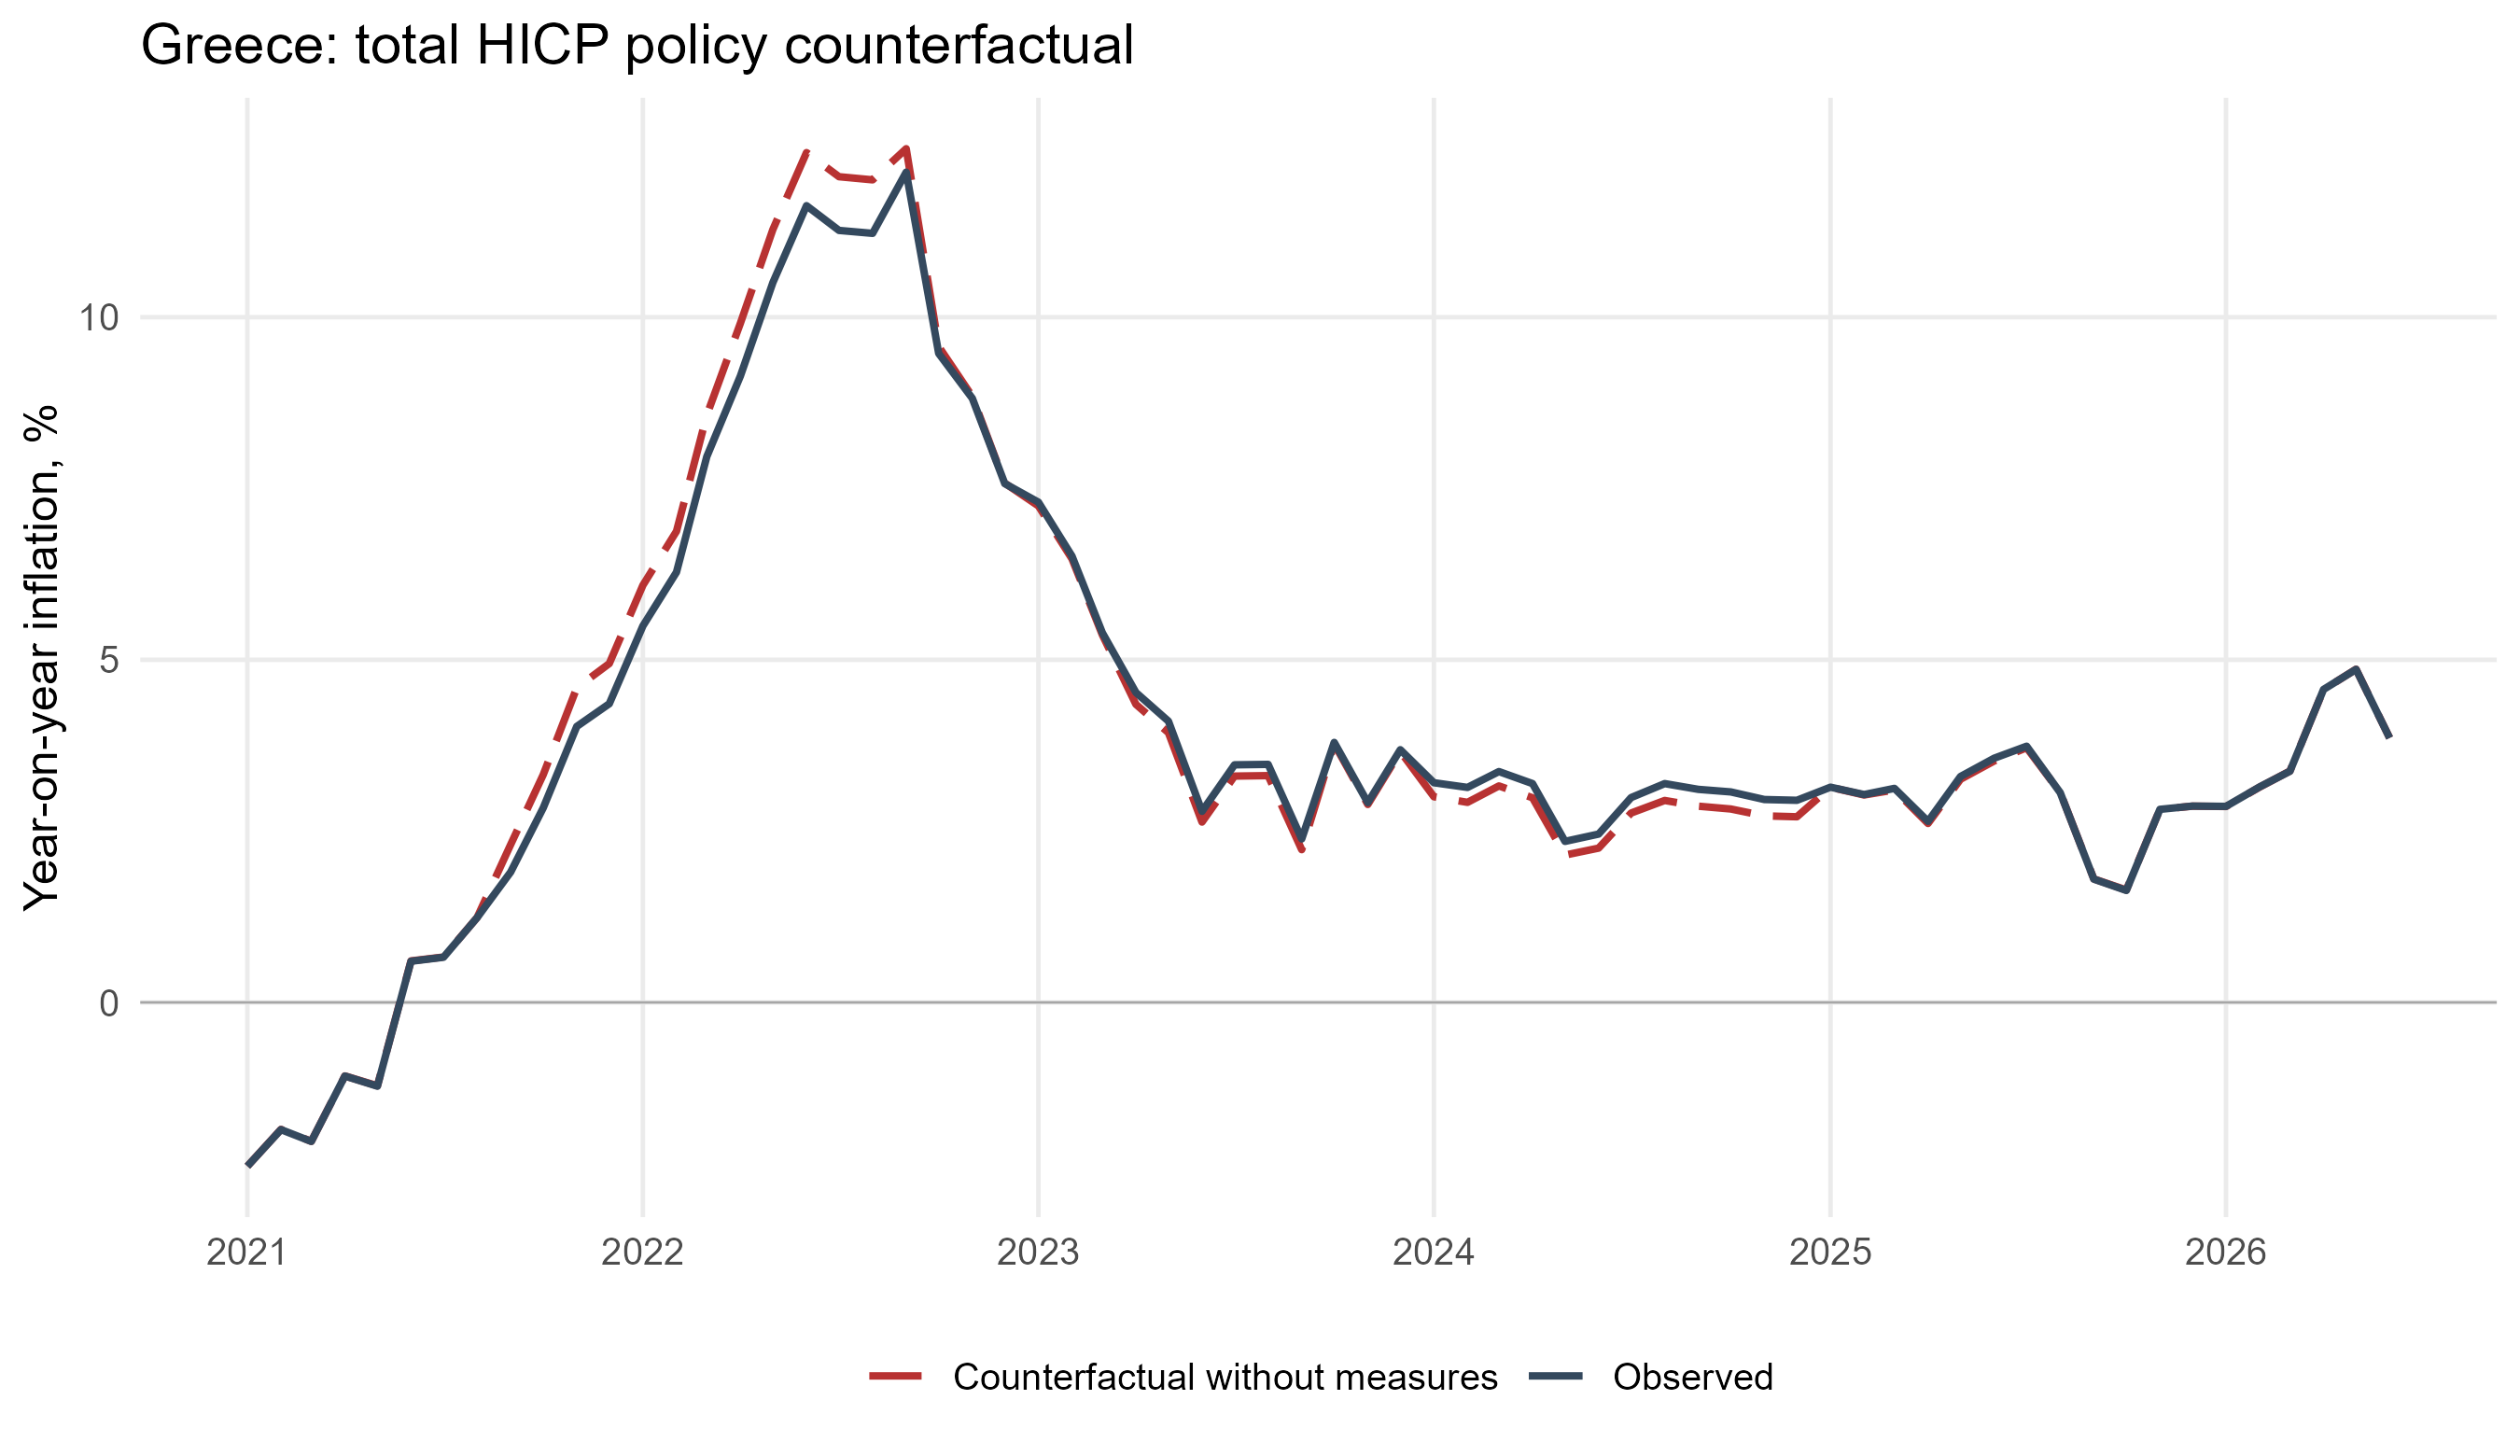
\includegraphics[width=0.86\textwidth,height=0.38\textheight,keepaspectratio]{fig/policy_total_cpi_counterfactual_inflation_EL_greece.png}
\caption{Greece: observed and counterfactual inflation}
\end{figure}

\subsection{Spain}
\begin{figure}[H]
\centering
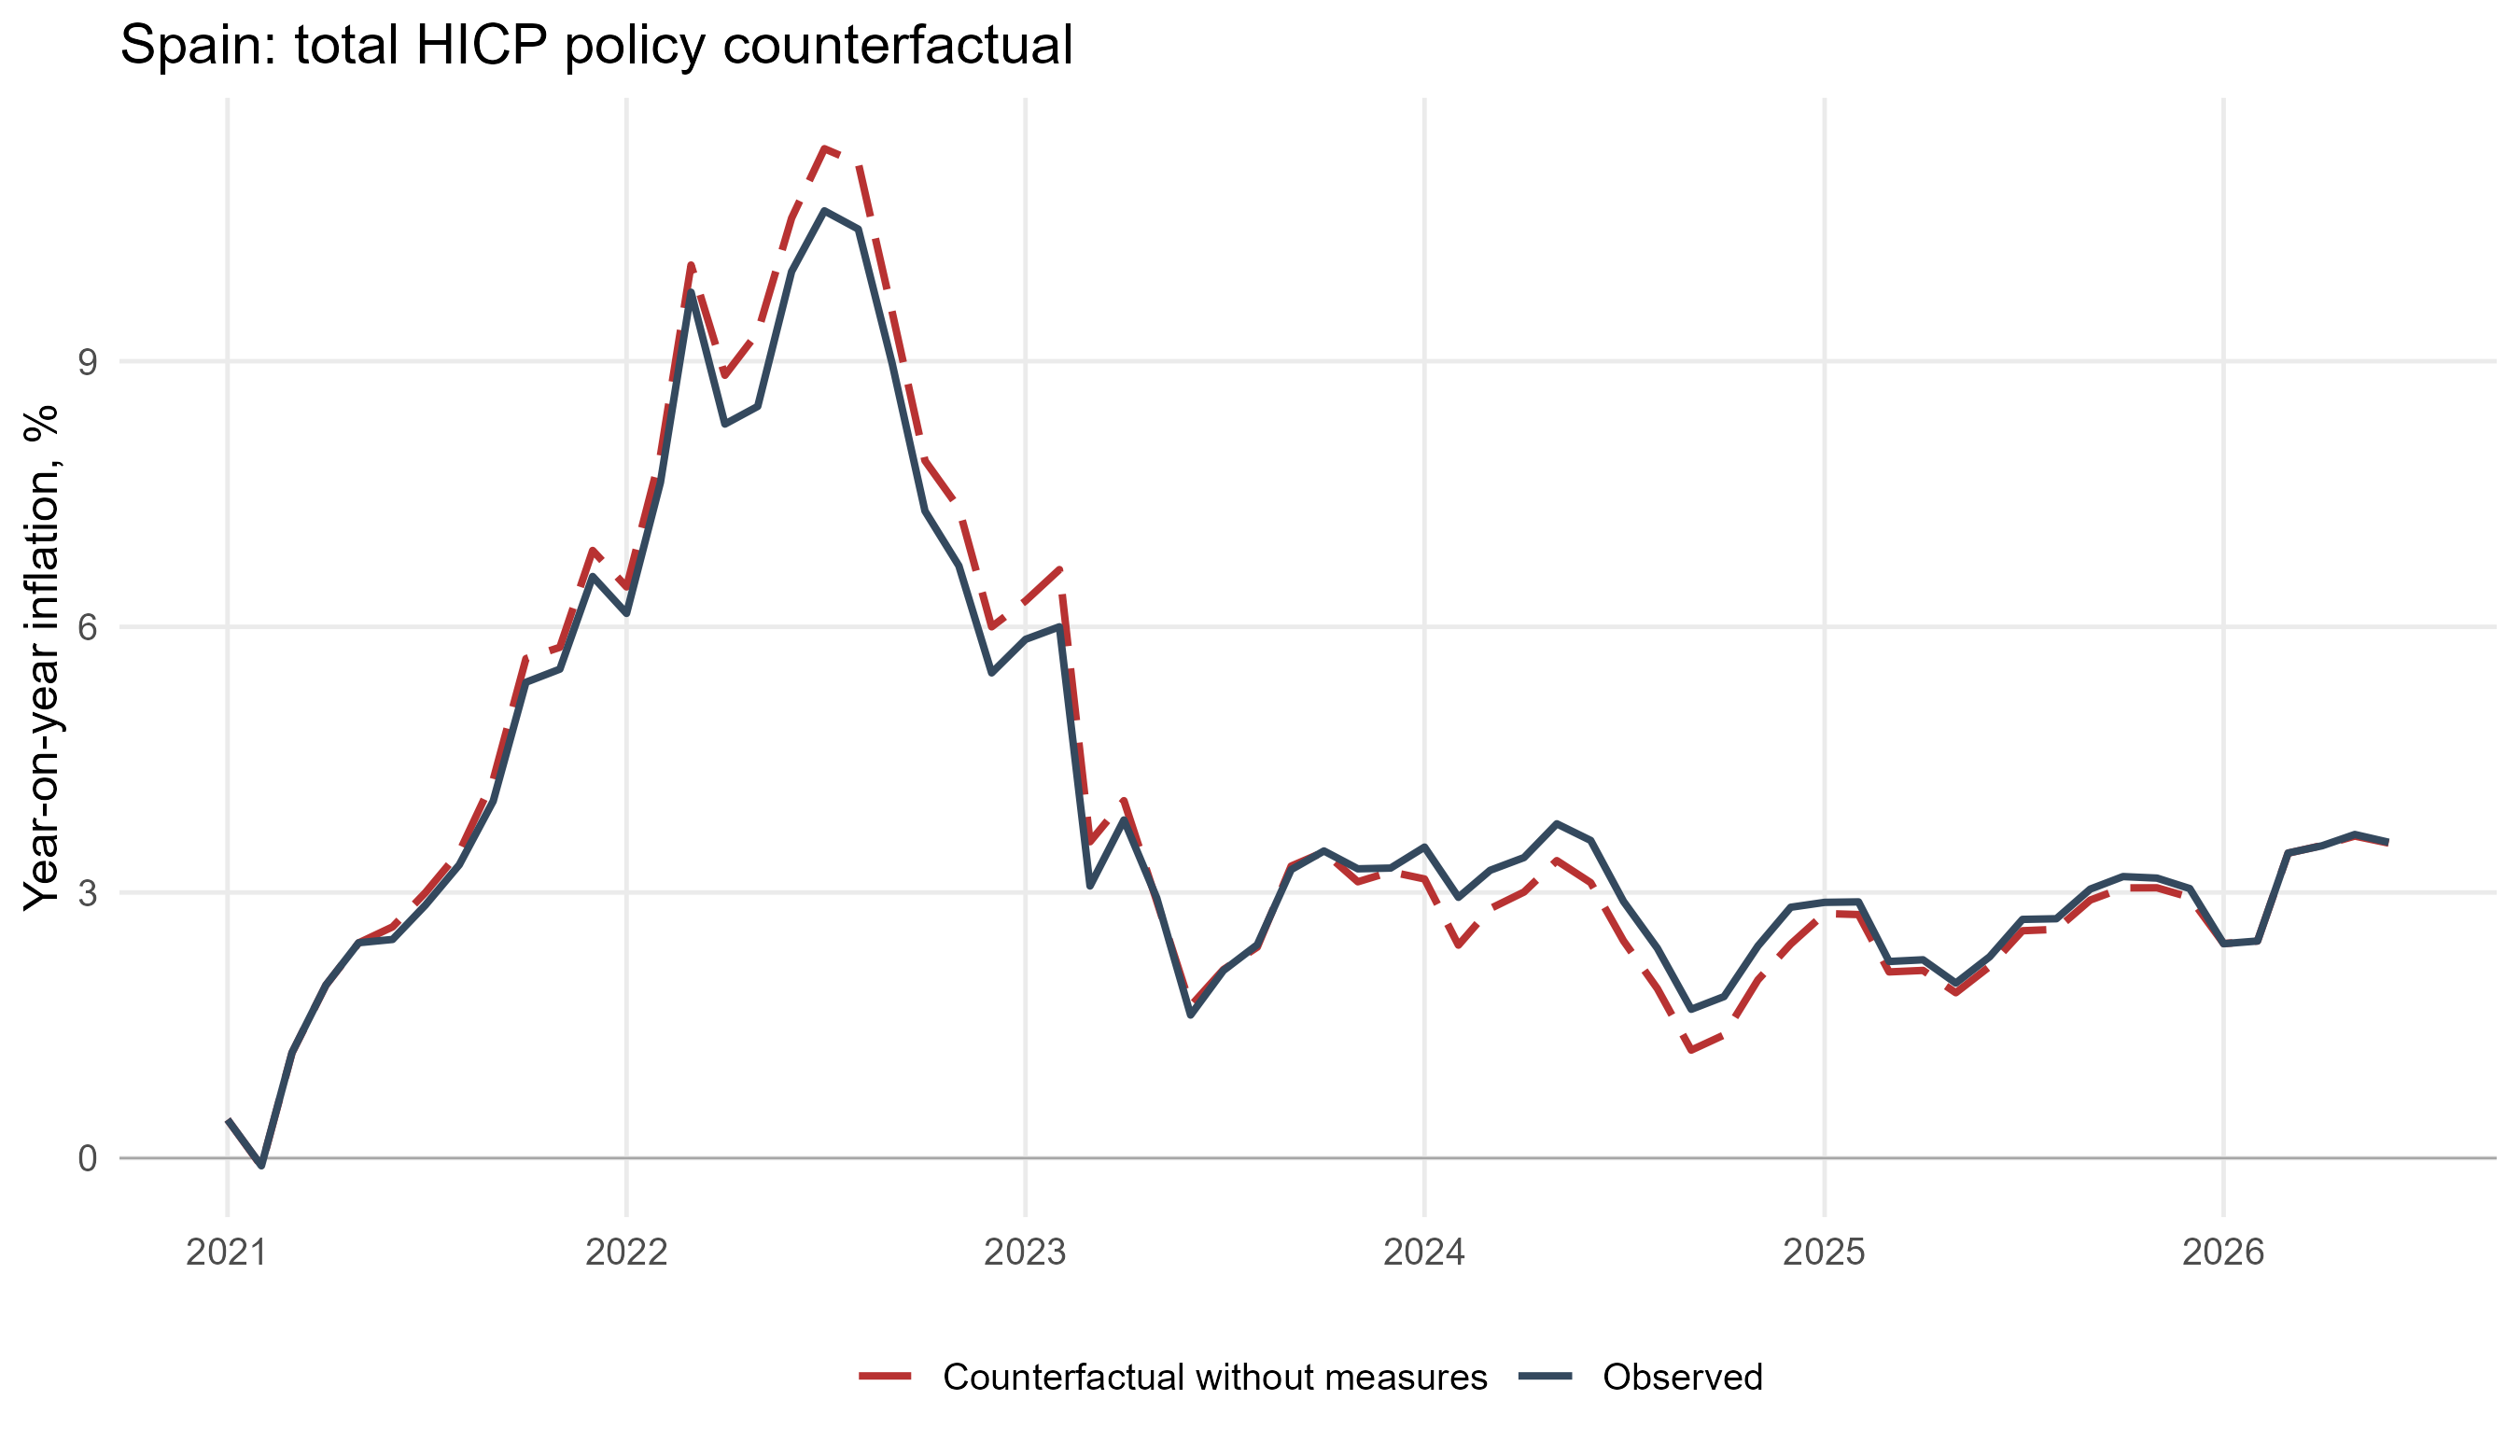
\includegraphics[width=0.86\textwidth,height=0.38\textheight,keepaspectratio]{fig/policy_total_cpi_counterfactual_inflation_ES_spain.png}
\caption{Spain: observed and counterfactual inflation}
\end{figure}

\subsection{Finland}
\begin{figure}[H]
\centering
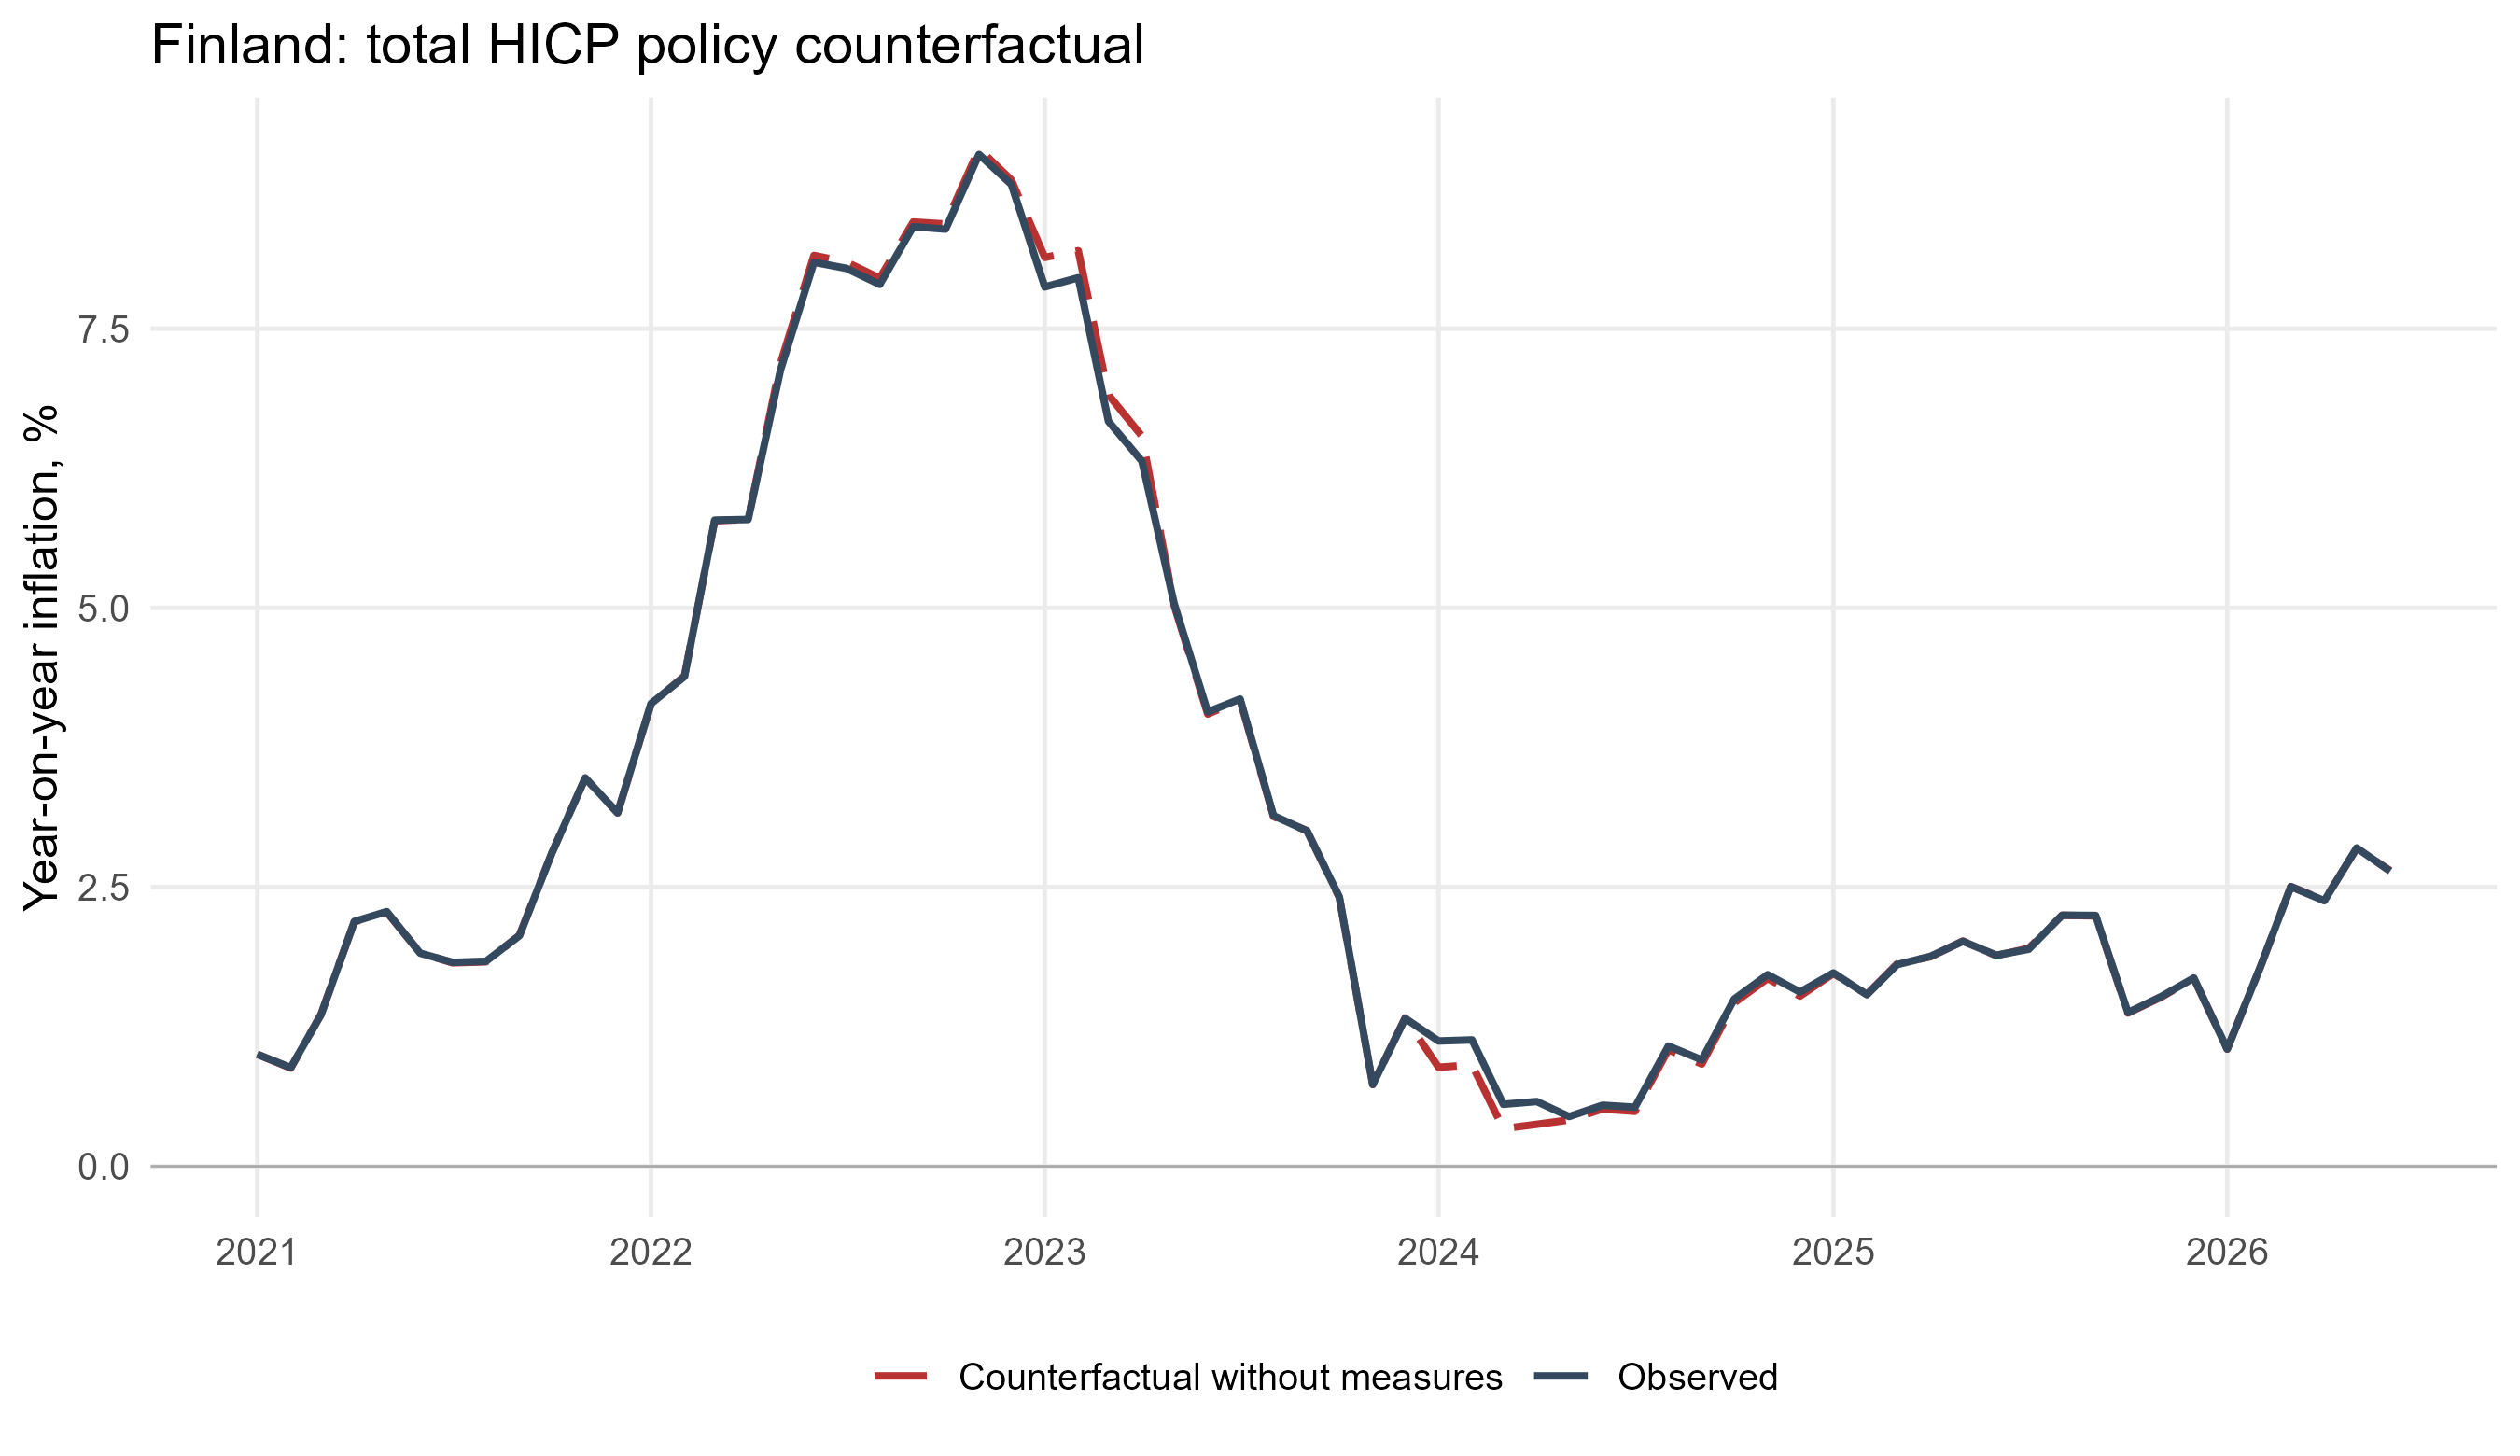
\includegraphics[width=0.86\textwidth,height=0.38\textheight,keepaspectratio]{fig/policy_total_cpi_counterfactual_inflation_FI_finland.png}
\caption{Finland: observed and counterfactual inflation}
\end{figure}

\subsection{France}
\begin{figure}[H]
\centering
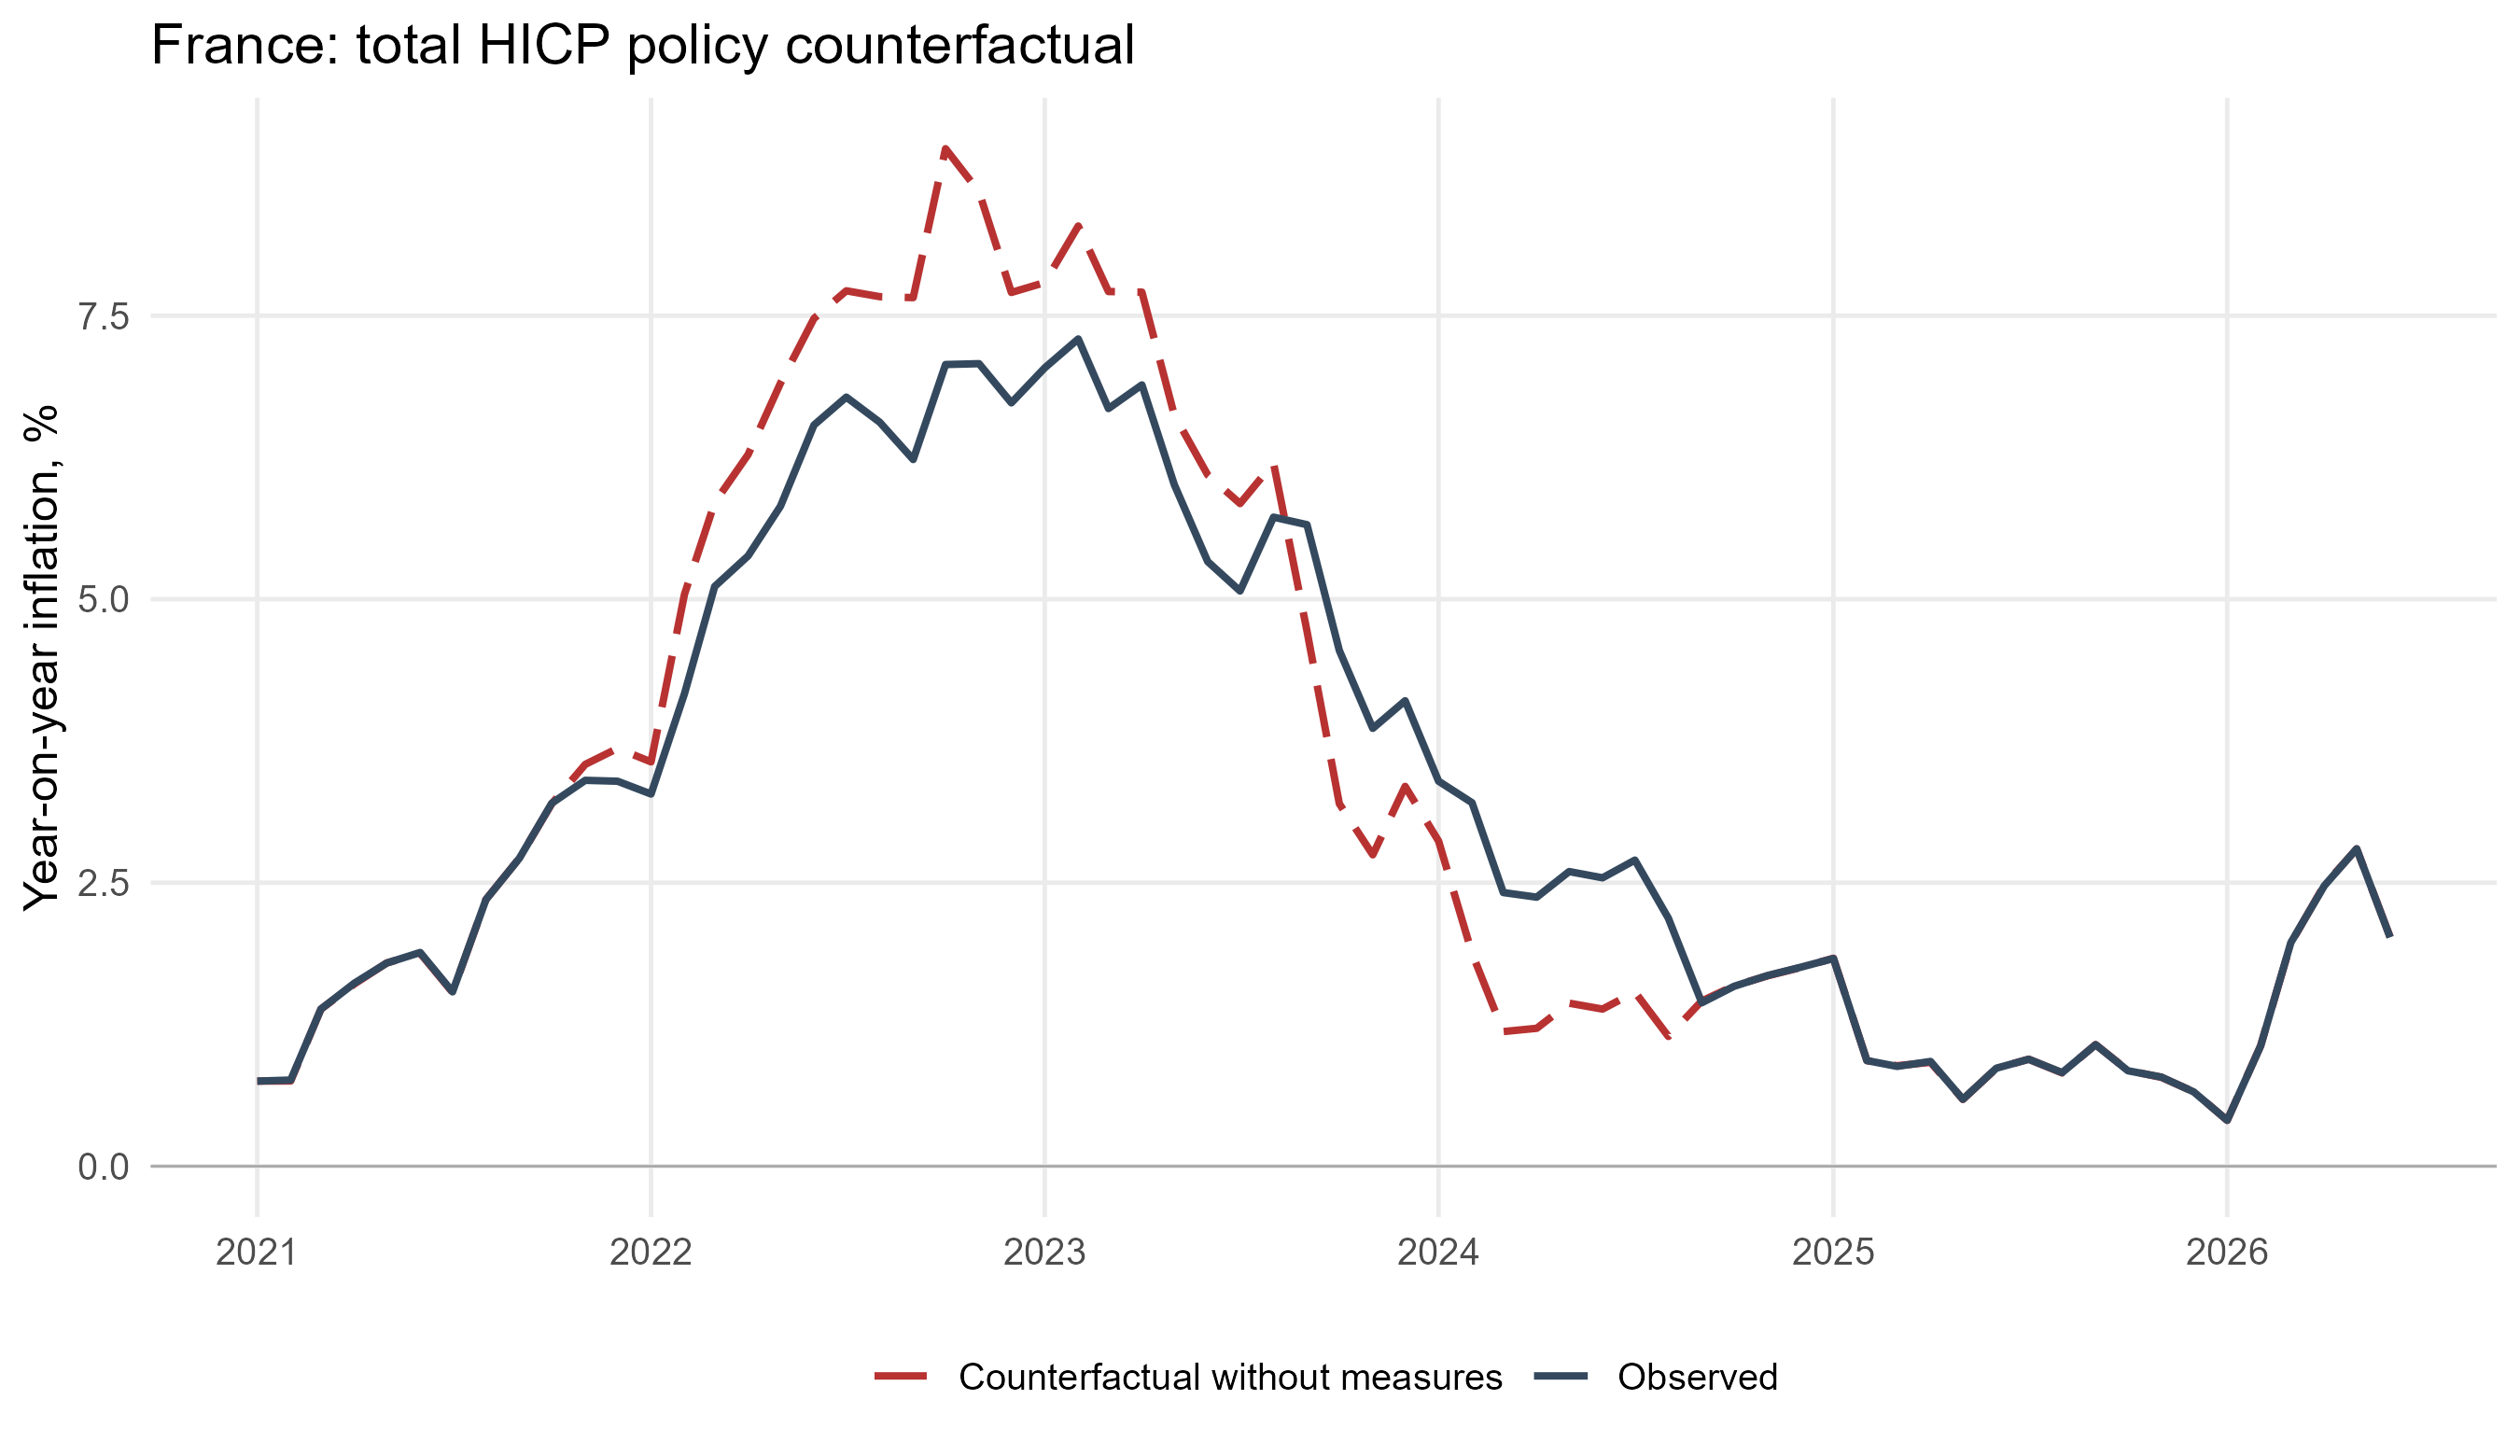
\includegraphics[width=0.86\textwidth,height=0.38\textheight,keepaspectratio]{fig/policy_total_cpi_counterfactual_inflation_FR_france.png}
\caption{France: observed and counterfactual inflation}
\end{figure}

\subsection{Croatia}
\begin{figure}[H]
\centering
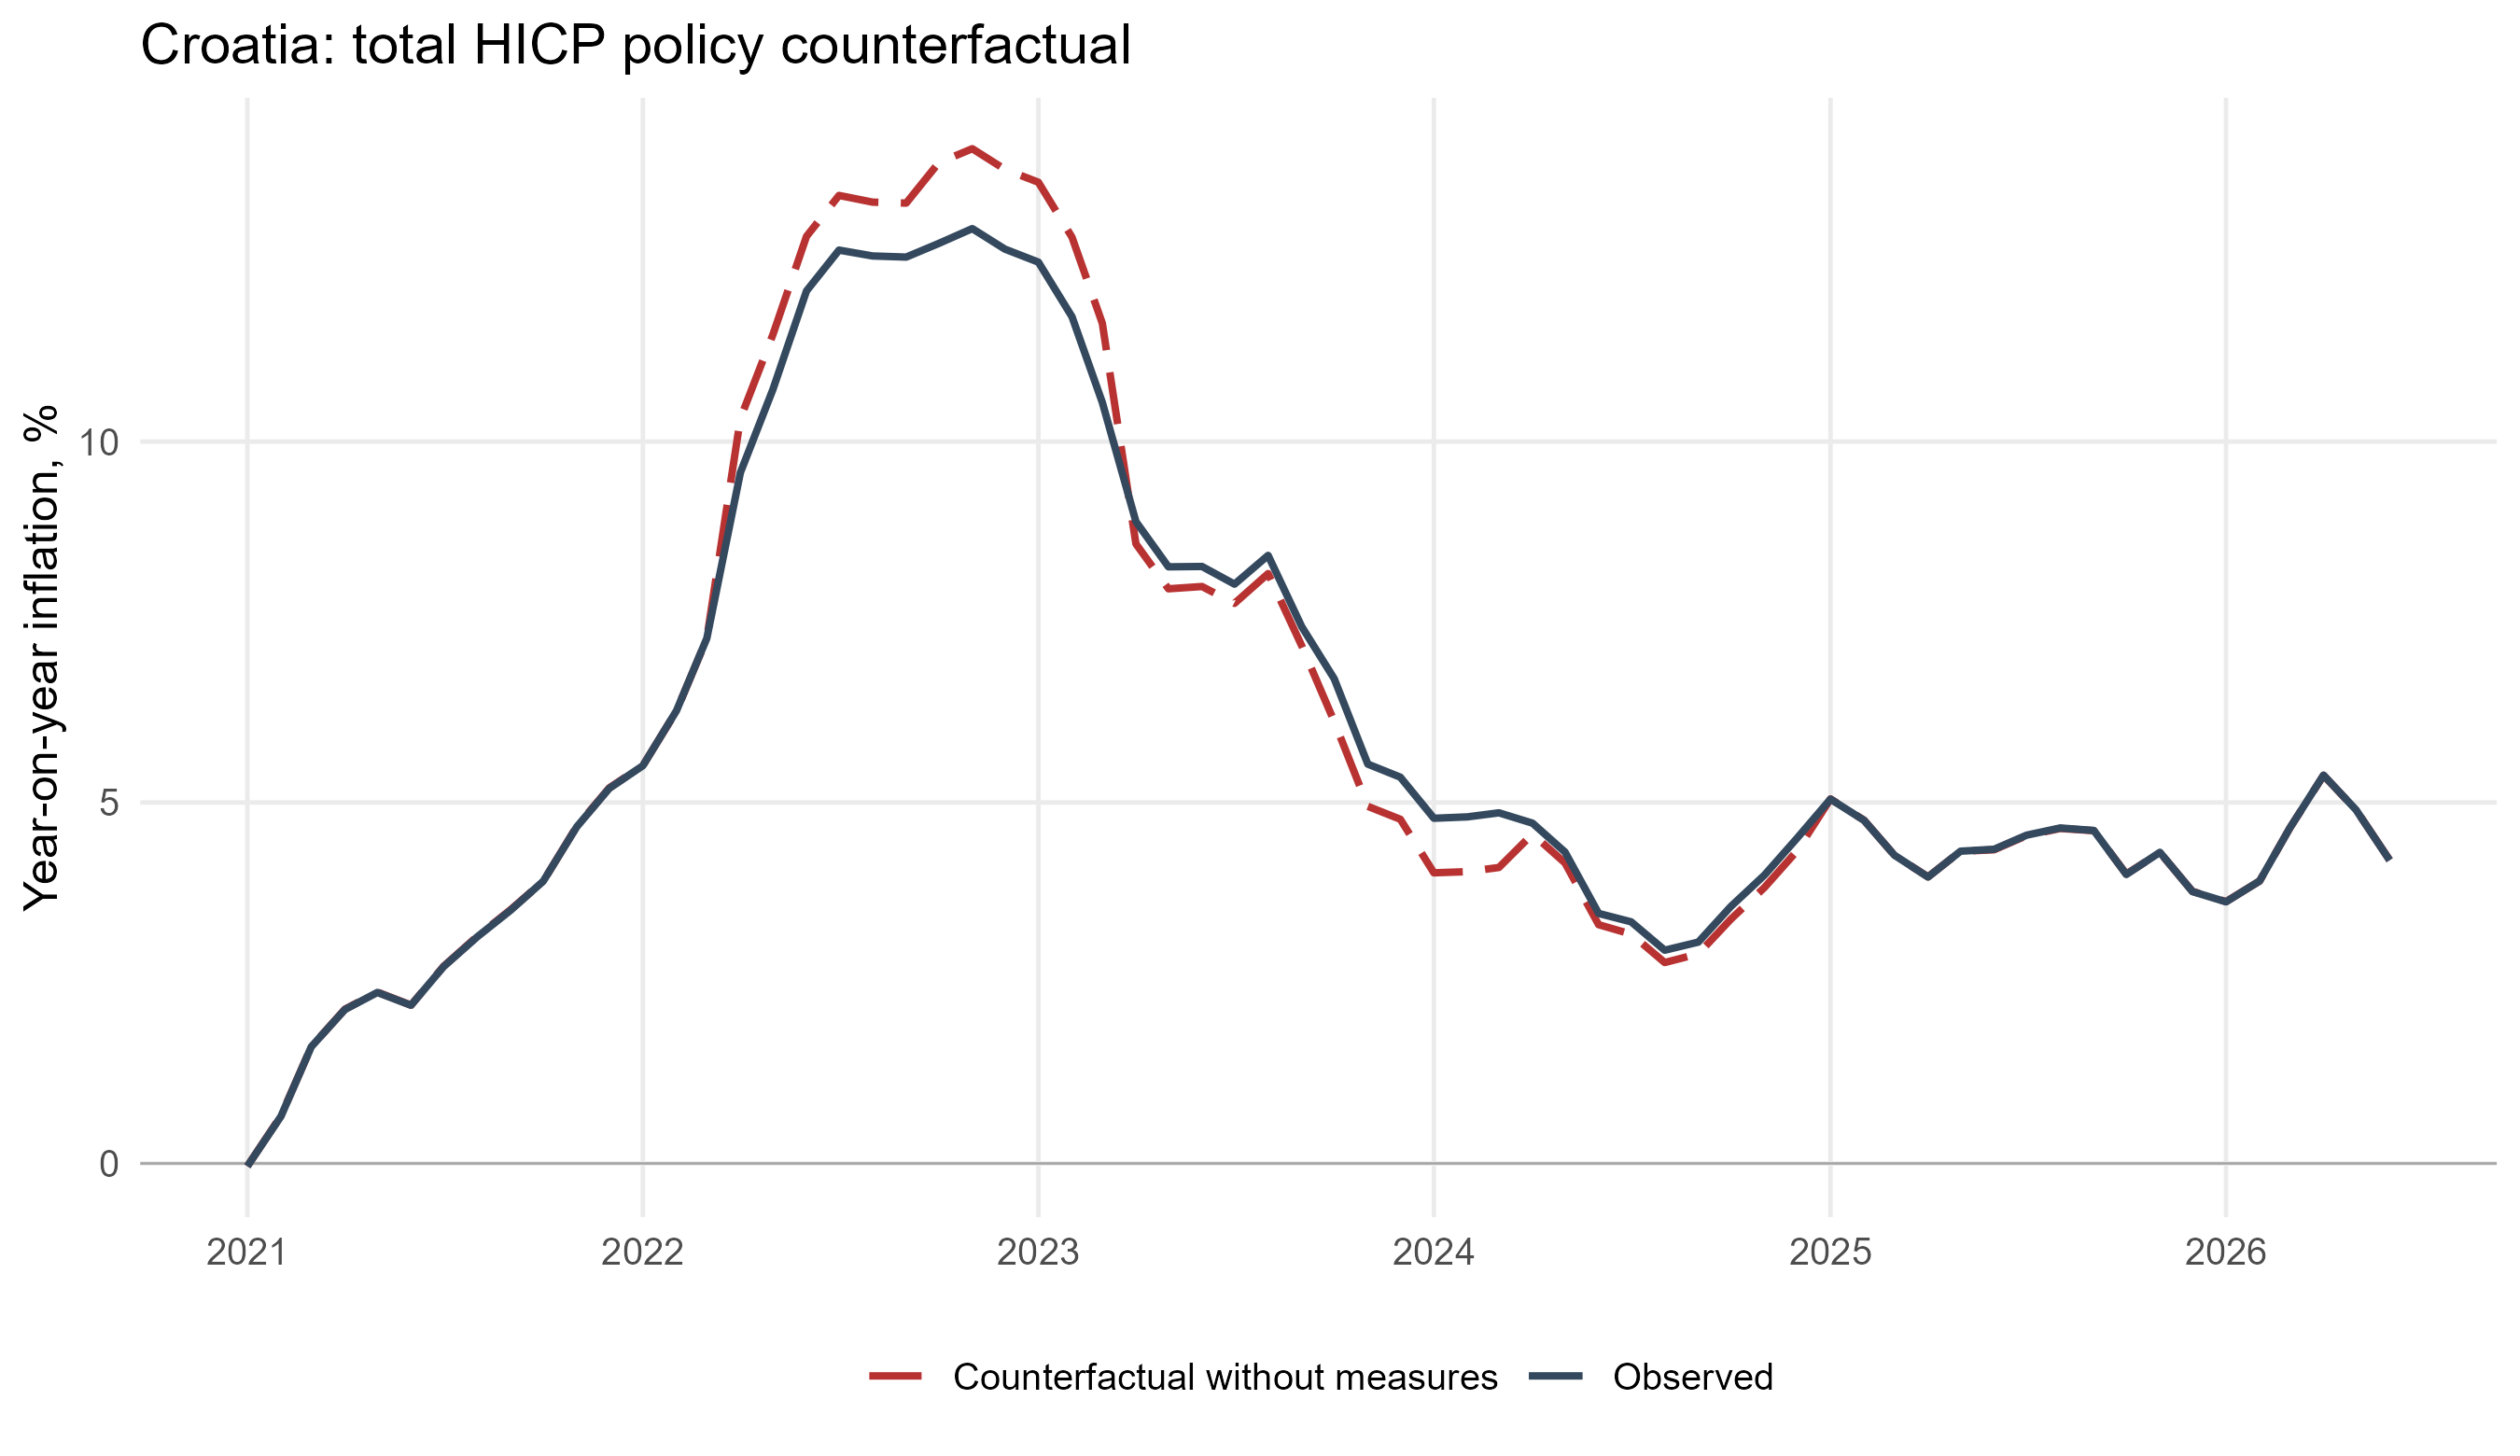
\includegraphics[width=0.86\textwidth,height=0.38\textheight,keepaspectratio]{fig/policy_total_cpi_counterfactual_inflation_HR_croatia.png}
\caption{Croatia: observed and counterfactual inflation}
\end{figure}

\subsection{Ireland}
\begin{figure}[H]
\centering
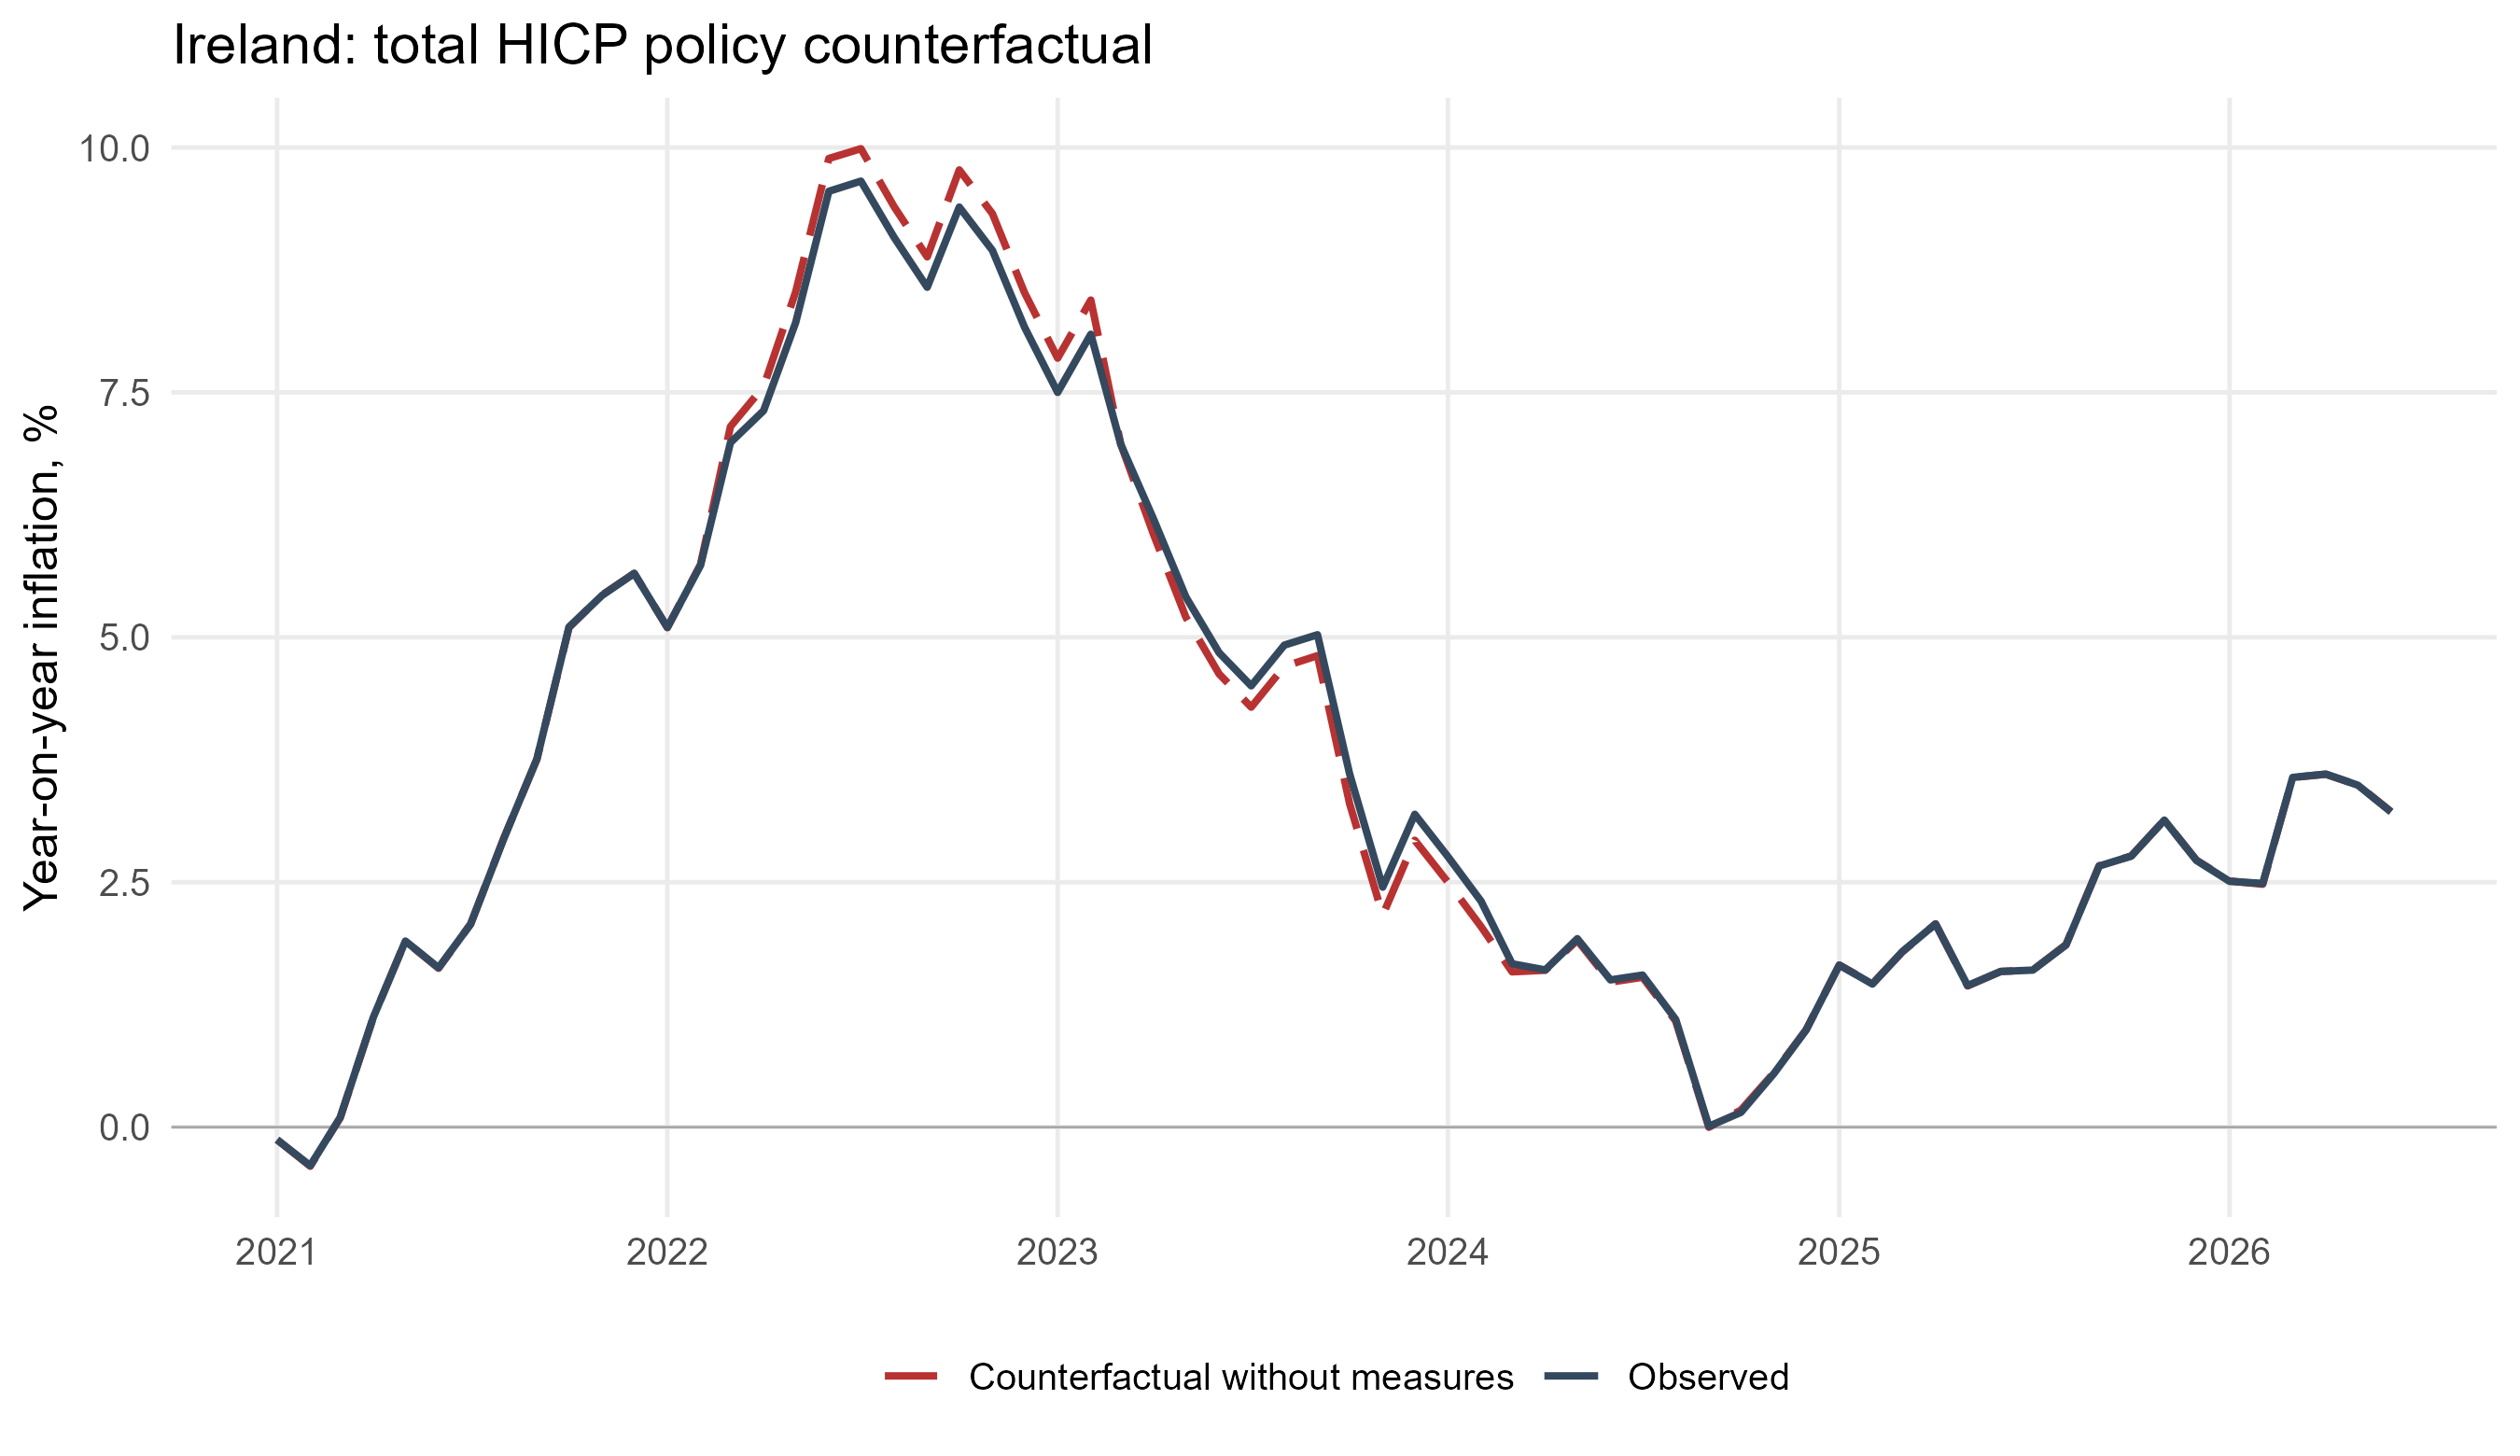
\includegraphics[width=0.86\textwidth,height=0.38\textheight,keepaspectratio]{fig/policy_total_cpi_counterfactual_inflation_IE_ireland.png}
\caption{Ireland: observed and counterfactual inflation}
\end{figure}

\subsection{Italy}
\begin{figure}[H]
\centering
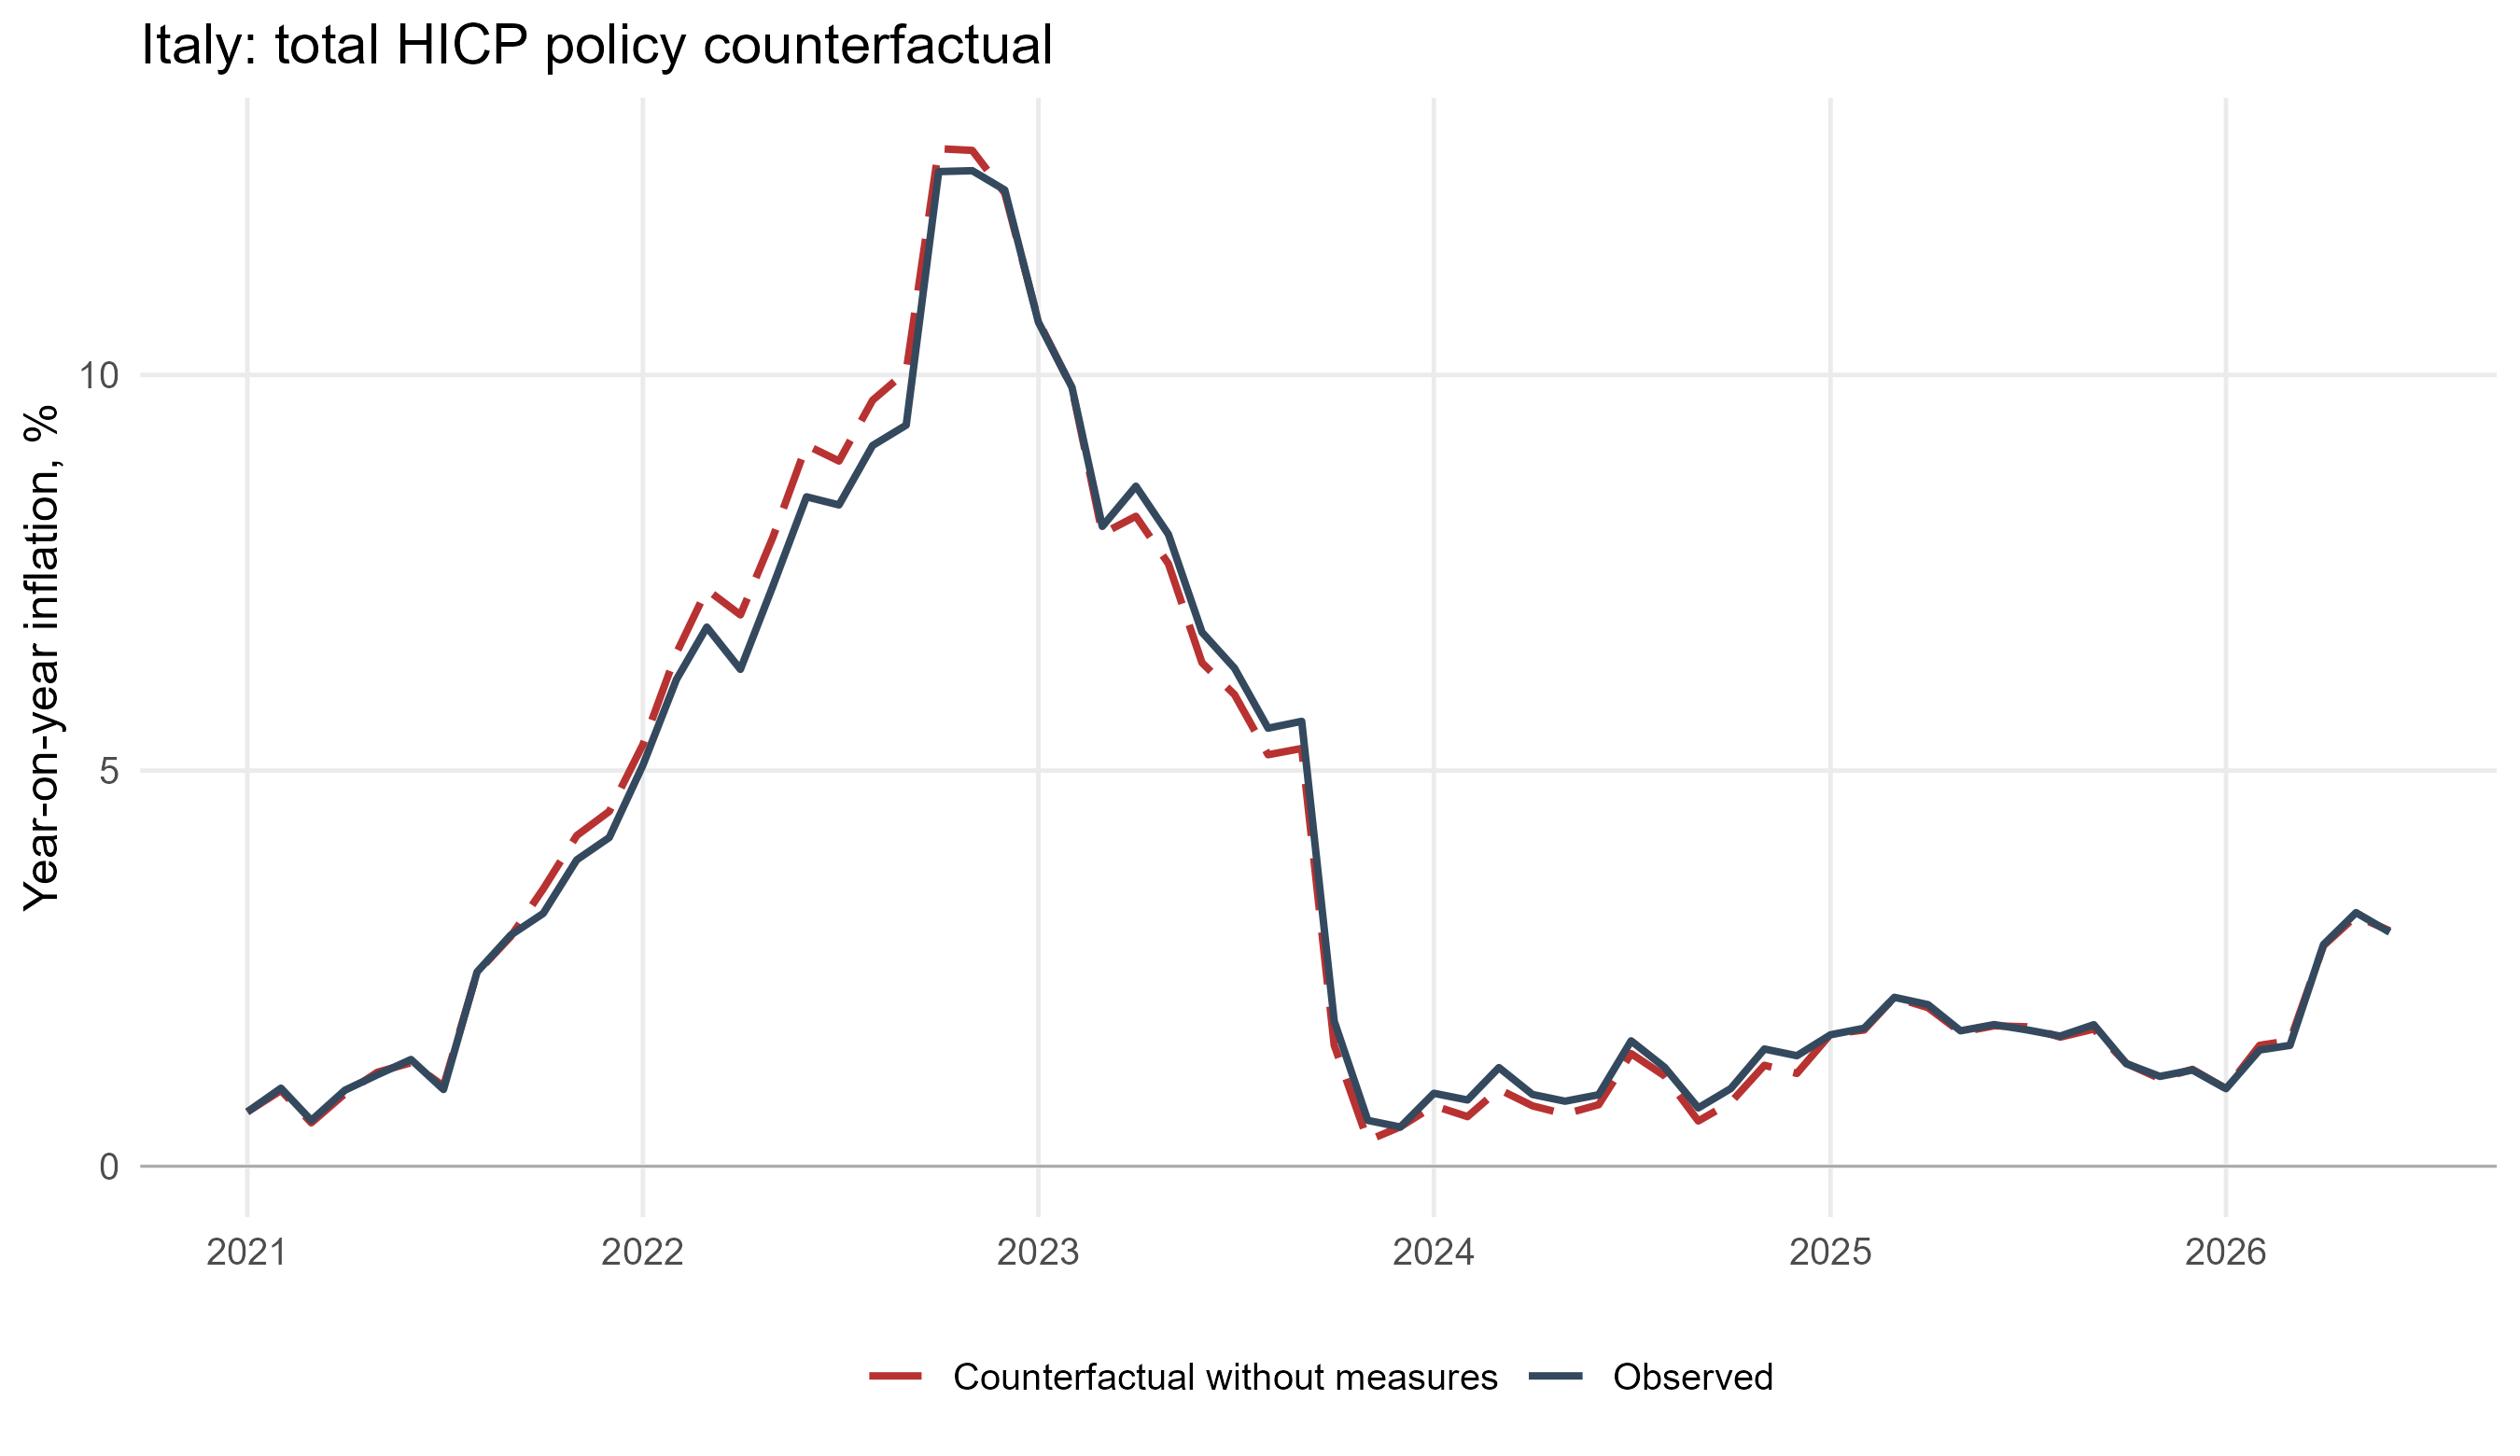
\includegraphics[width=0.86\textwidth,height=0.38\textheight,keepaspectratio]{fig/policy_total_cpi_counterfactual_inflation_IT_italy.png}
\caption{Italy: observed and counterfactual inflation}
\end{figure}

\subsection{Lithuania}
\begin{figure}[H]
\centering
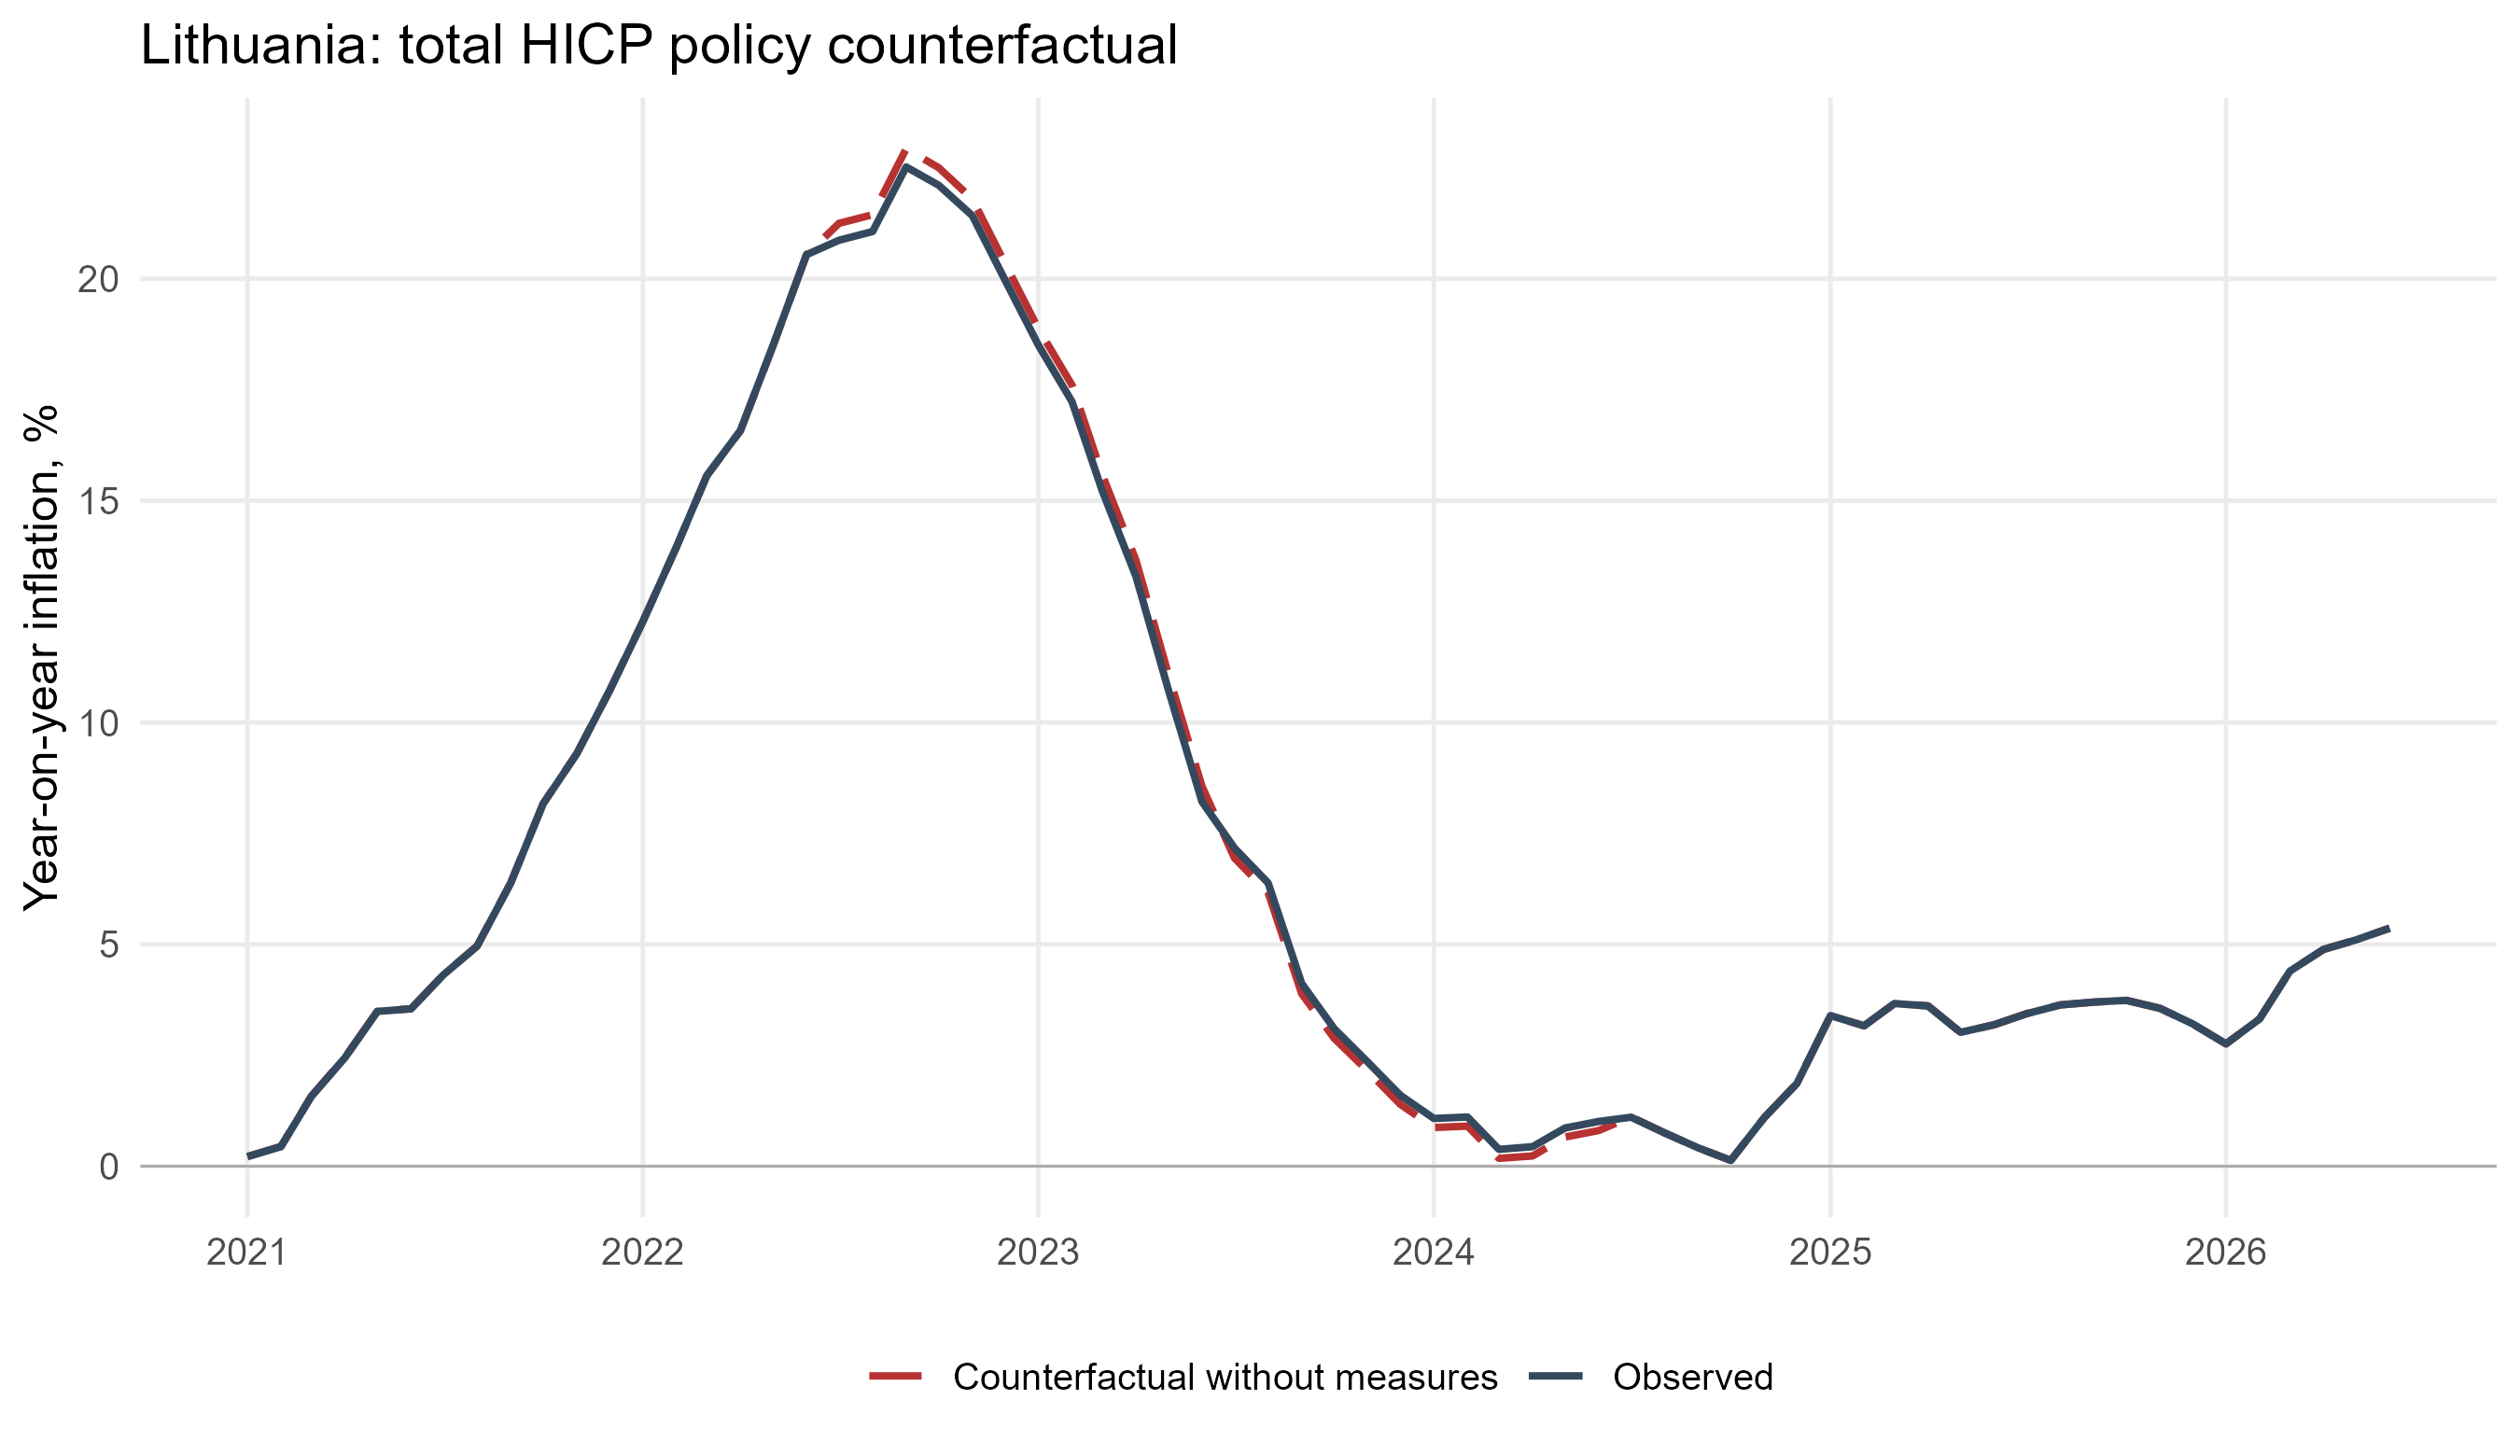
\includegraphics[width=0.86\textwidth,height=0.38\textheight,keepaspectratio]{fig/policy_total_cpi_counterfactual_inflation_LT_lithuania.png}
\caption{Lithuania: observed and counterfactual inflation}
\end{figure}

\subsection{Netherlands}
\begin{figure}[H]
\centering
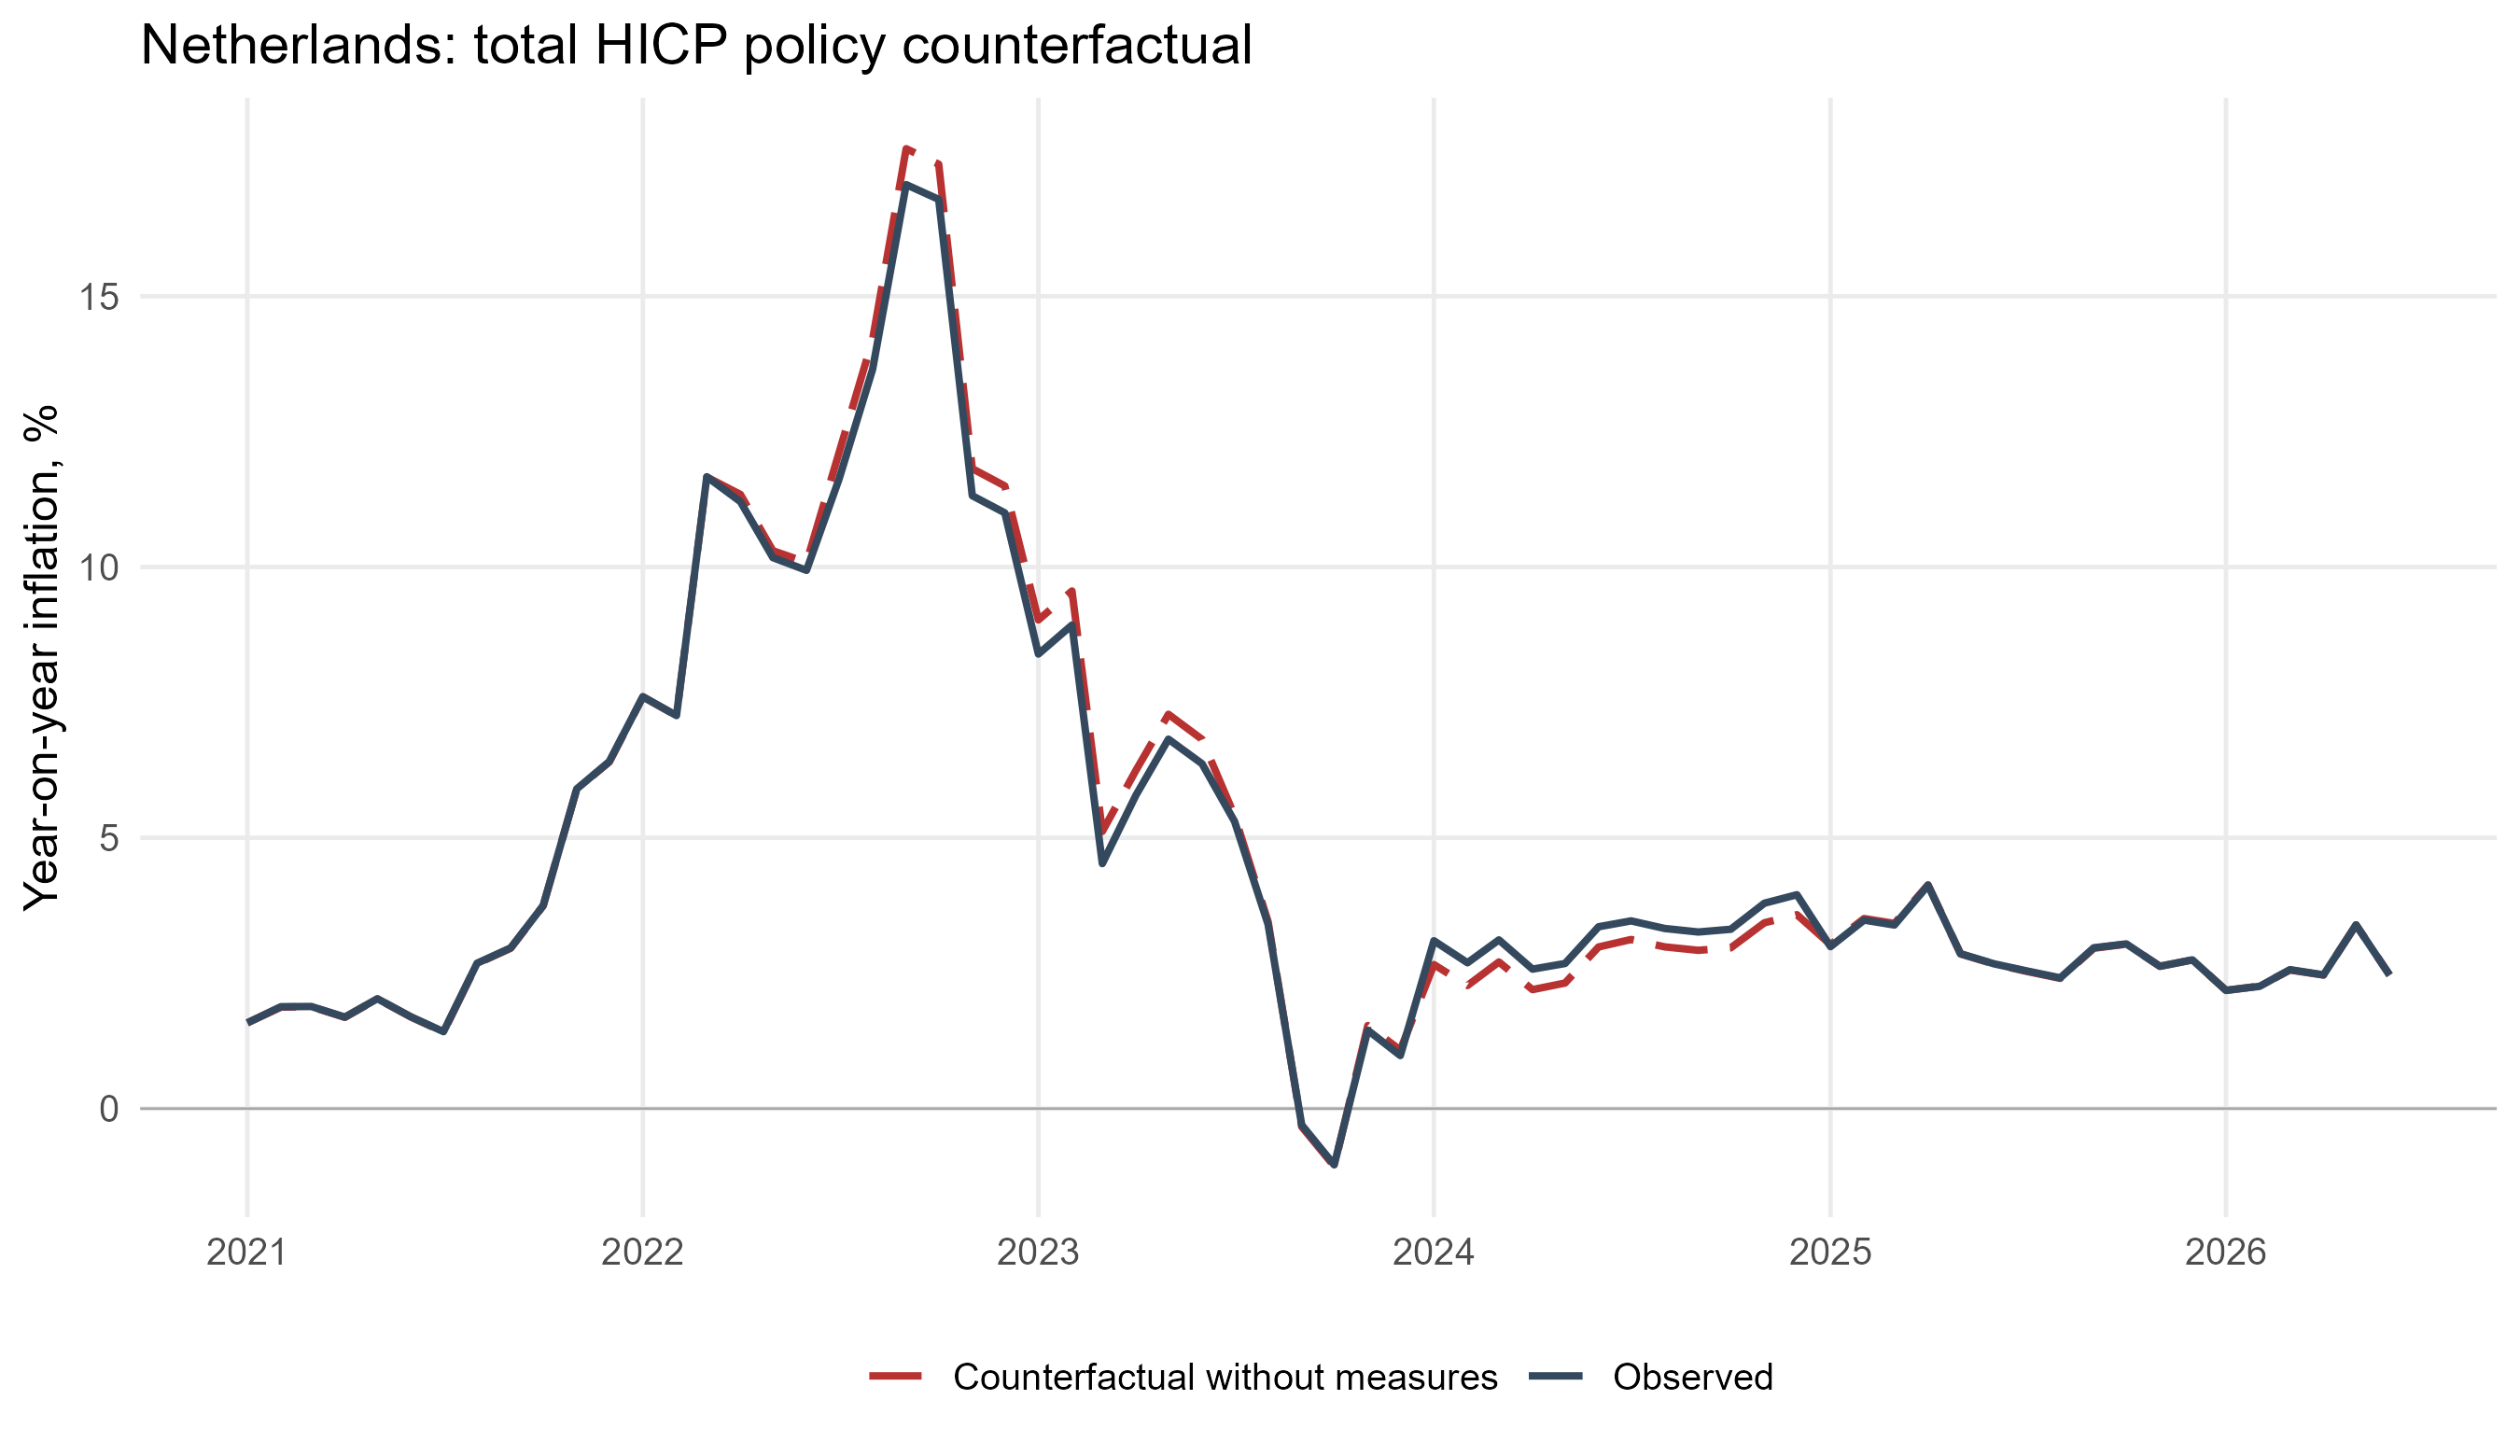
\includegraphics[width=0.86\textwidth,height=0.38\textheight,keepaspectratio]{fig/policy_total_cpi_counterfactual_inflation_NL_netherlands.png}
\caption{Netherlands: observed and counterfactual inflation}
\end{figure}

\subsection{Portugal}
\begin{figure}[H]
\centering
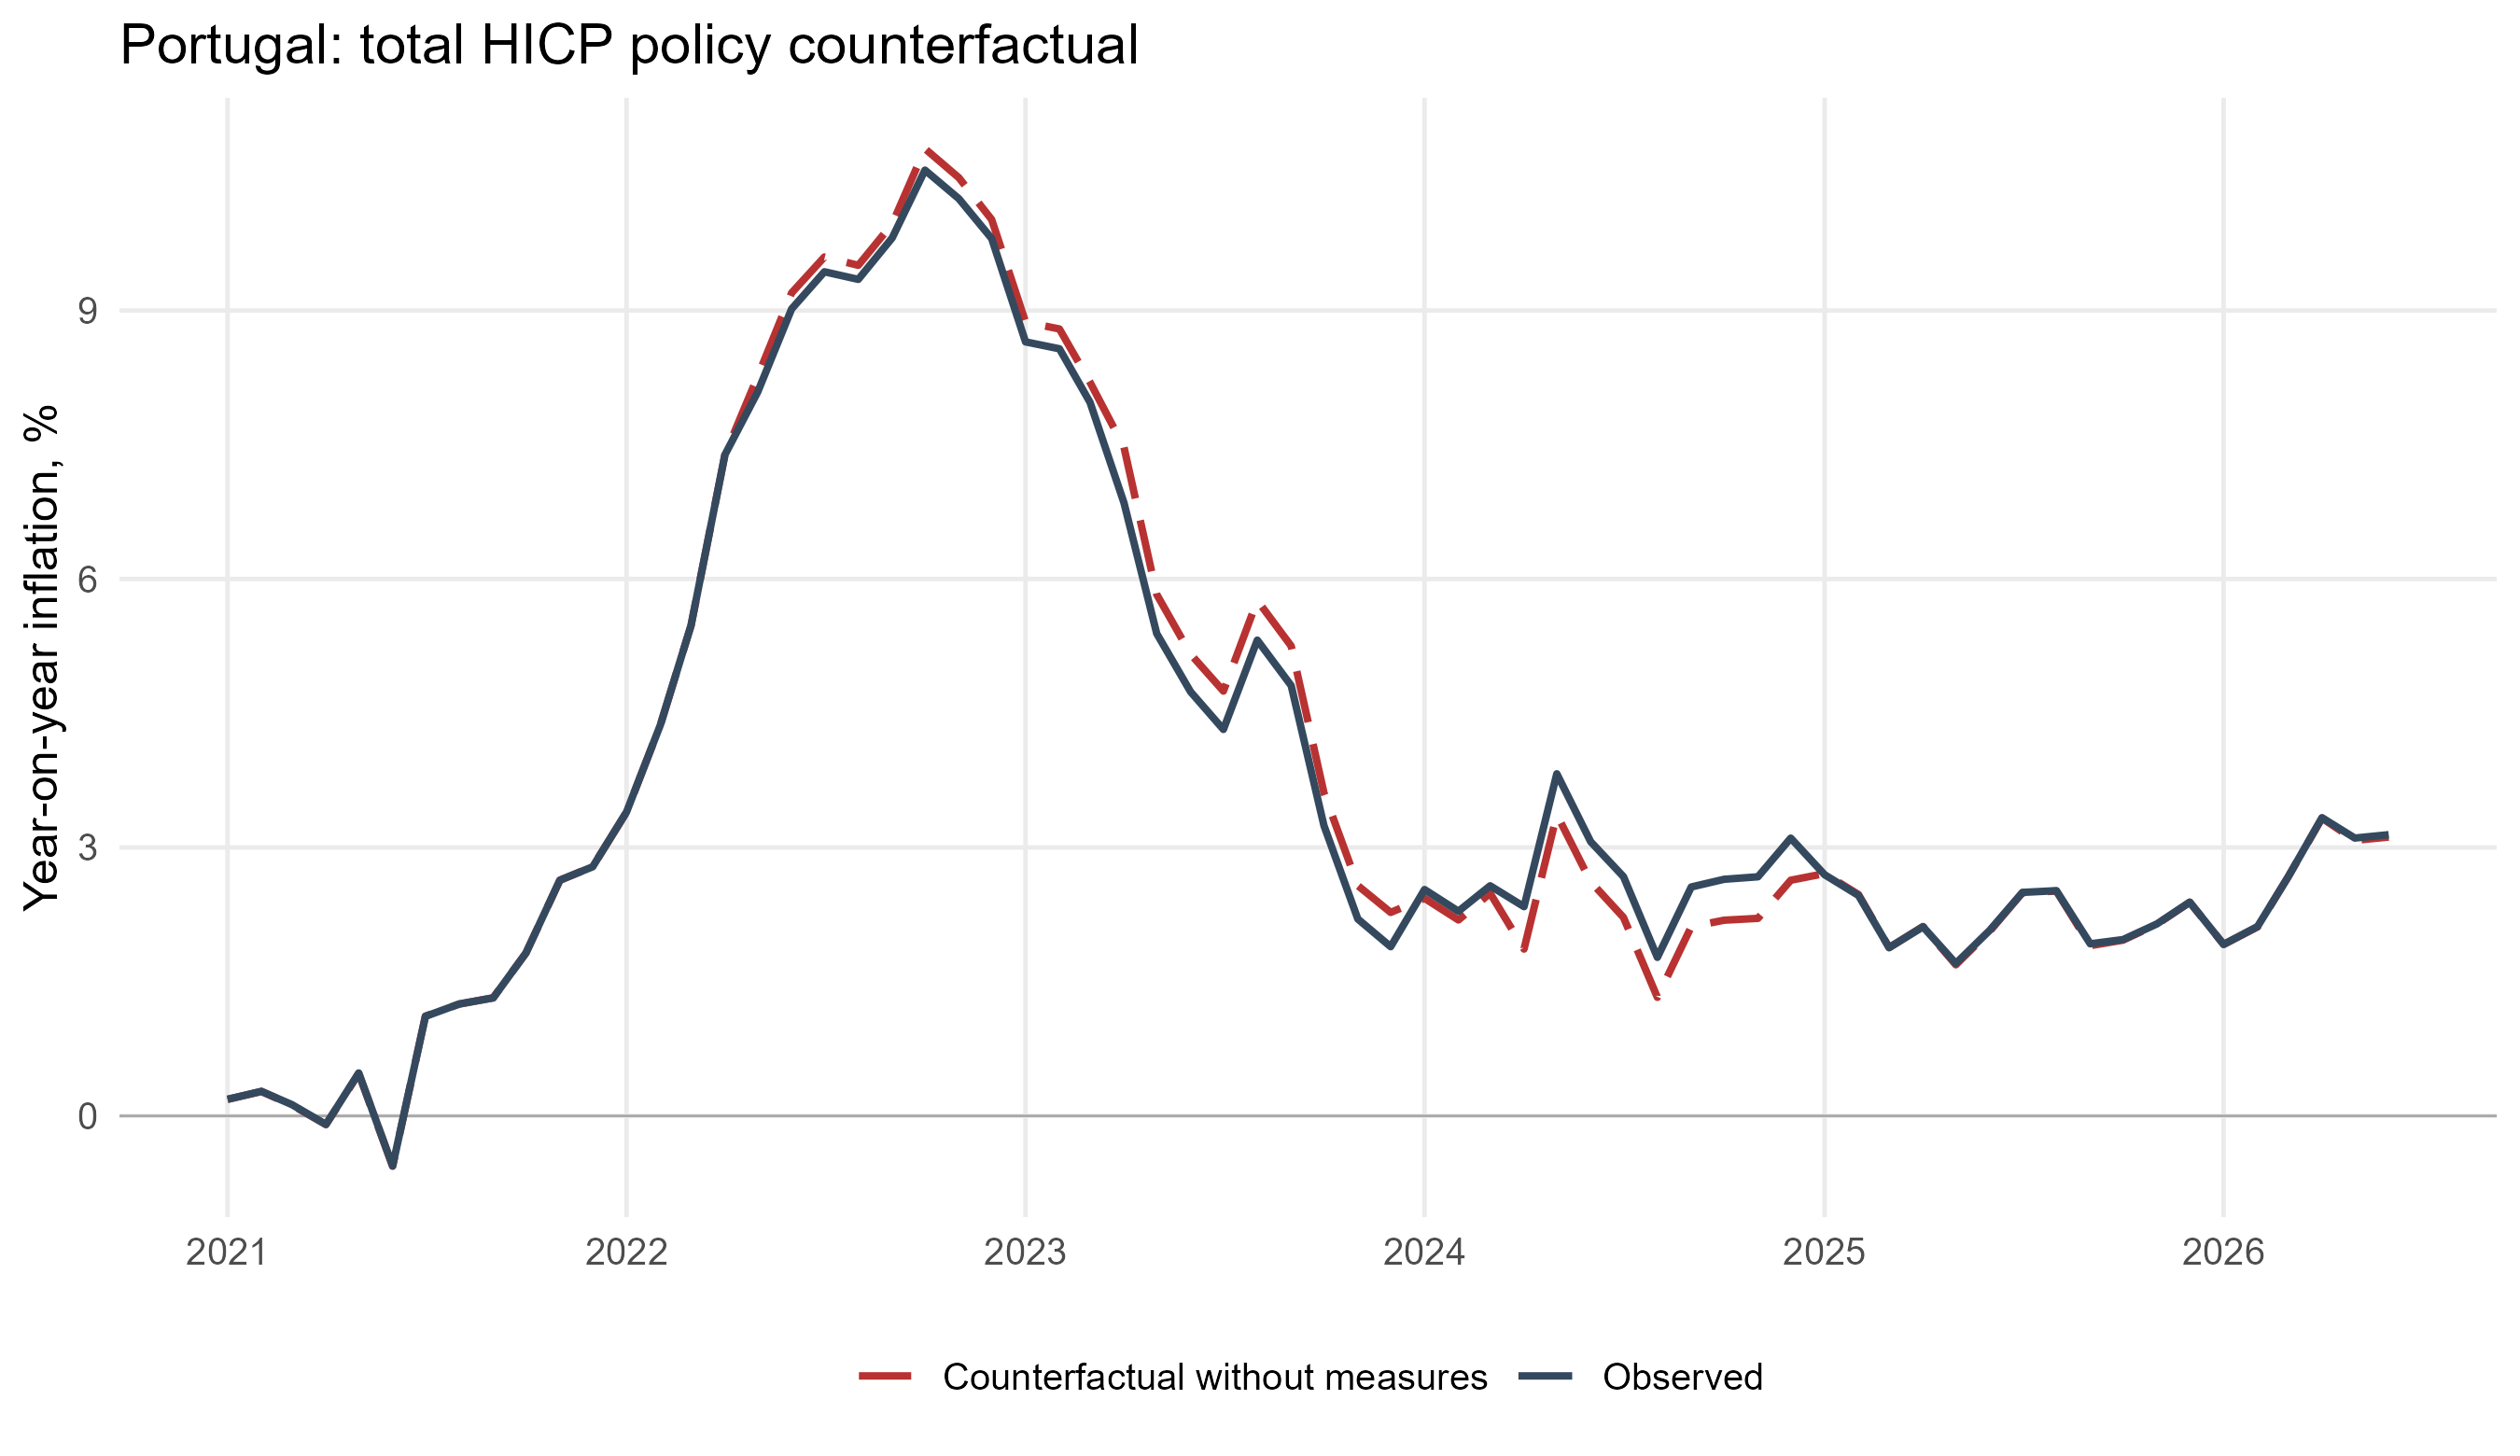
\includegraphics[width=0.86\textwidth,height=0.38\textheight,keepaspectratio]{fig/policy_total_cpi_counterfactual_inflation_PT_portugal.png}
\caption{Portugal: observed and counterfactual inflation}
\end{figure}

\subsection{Slovenia}
\begin{figure}[H]
\centering
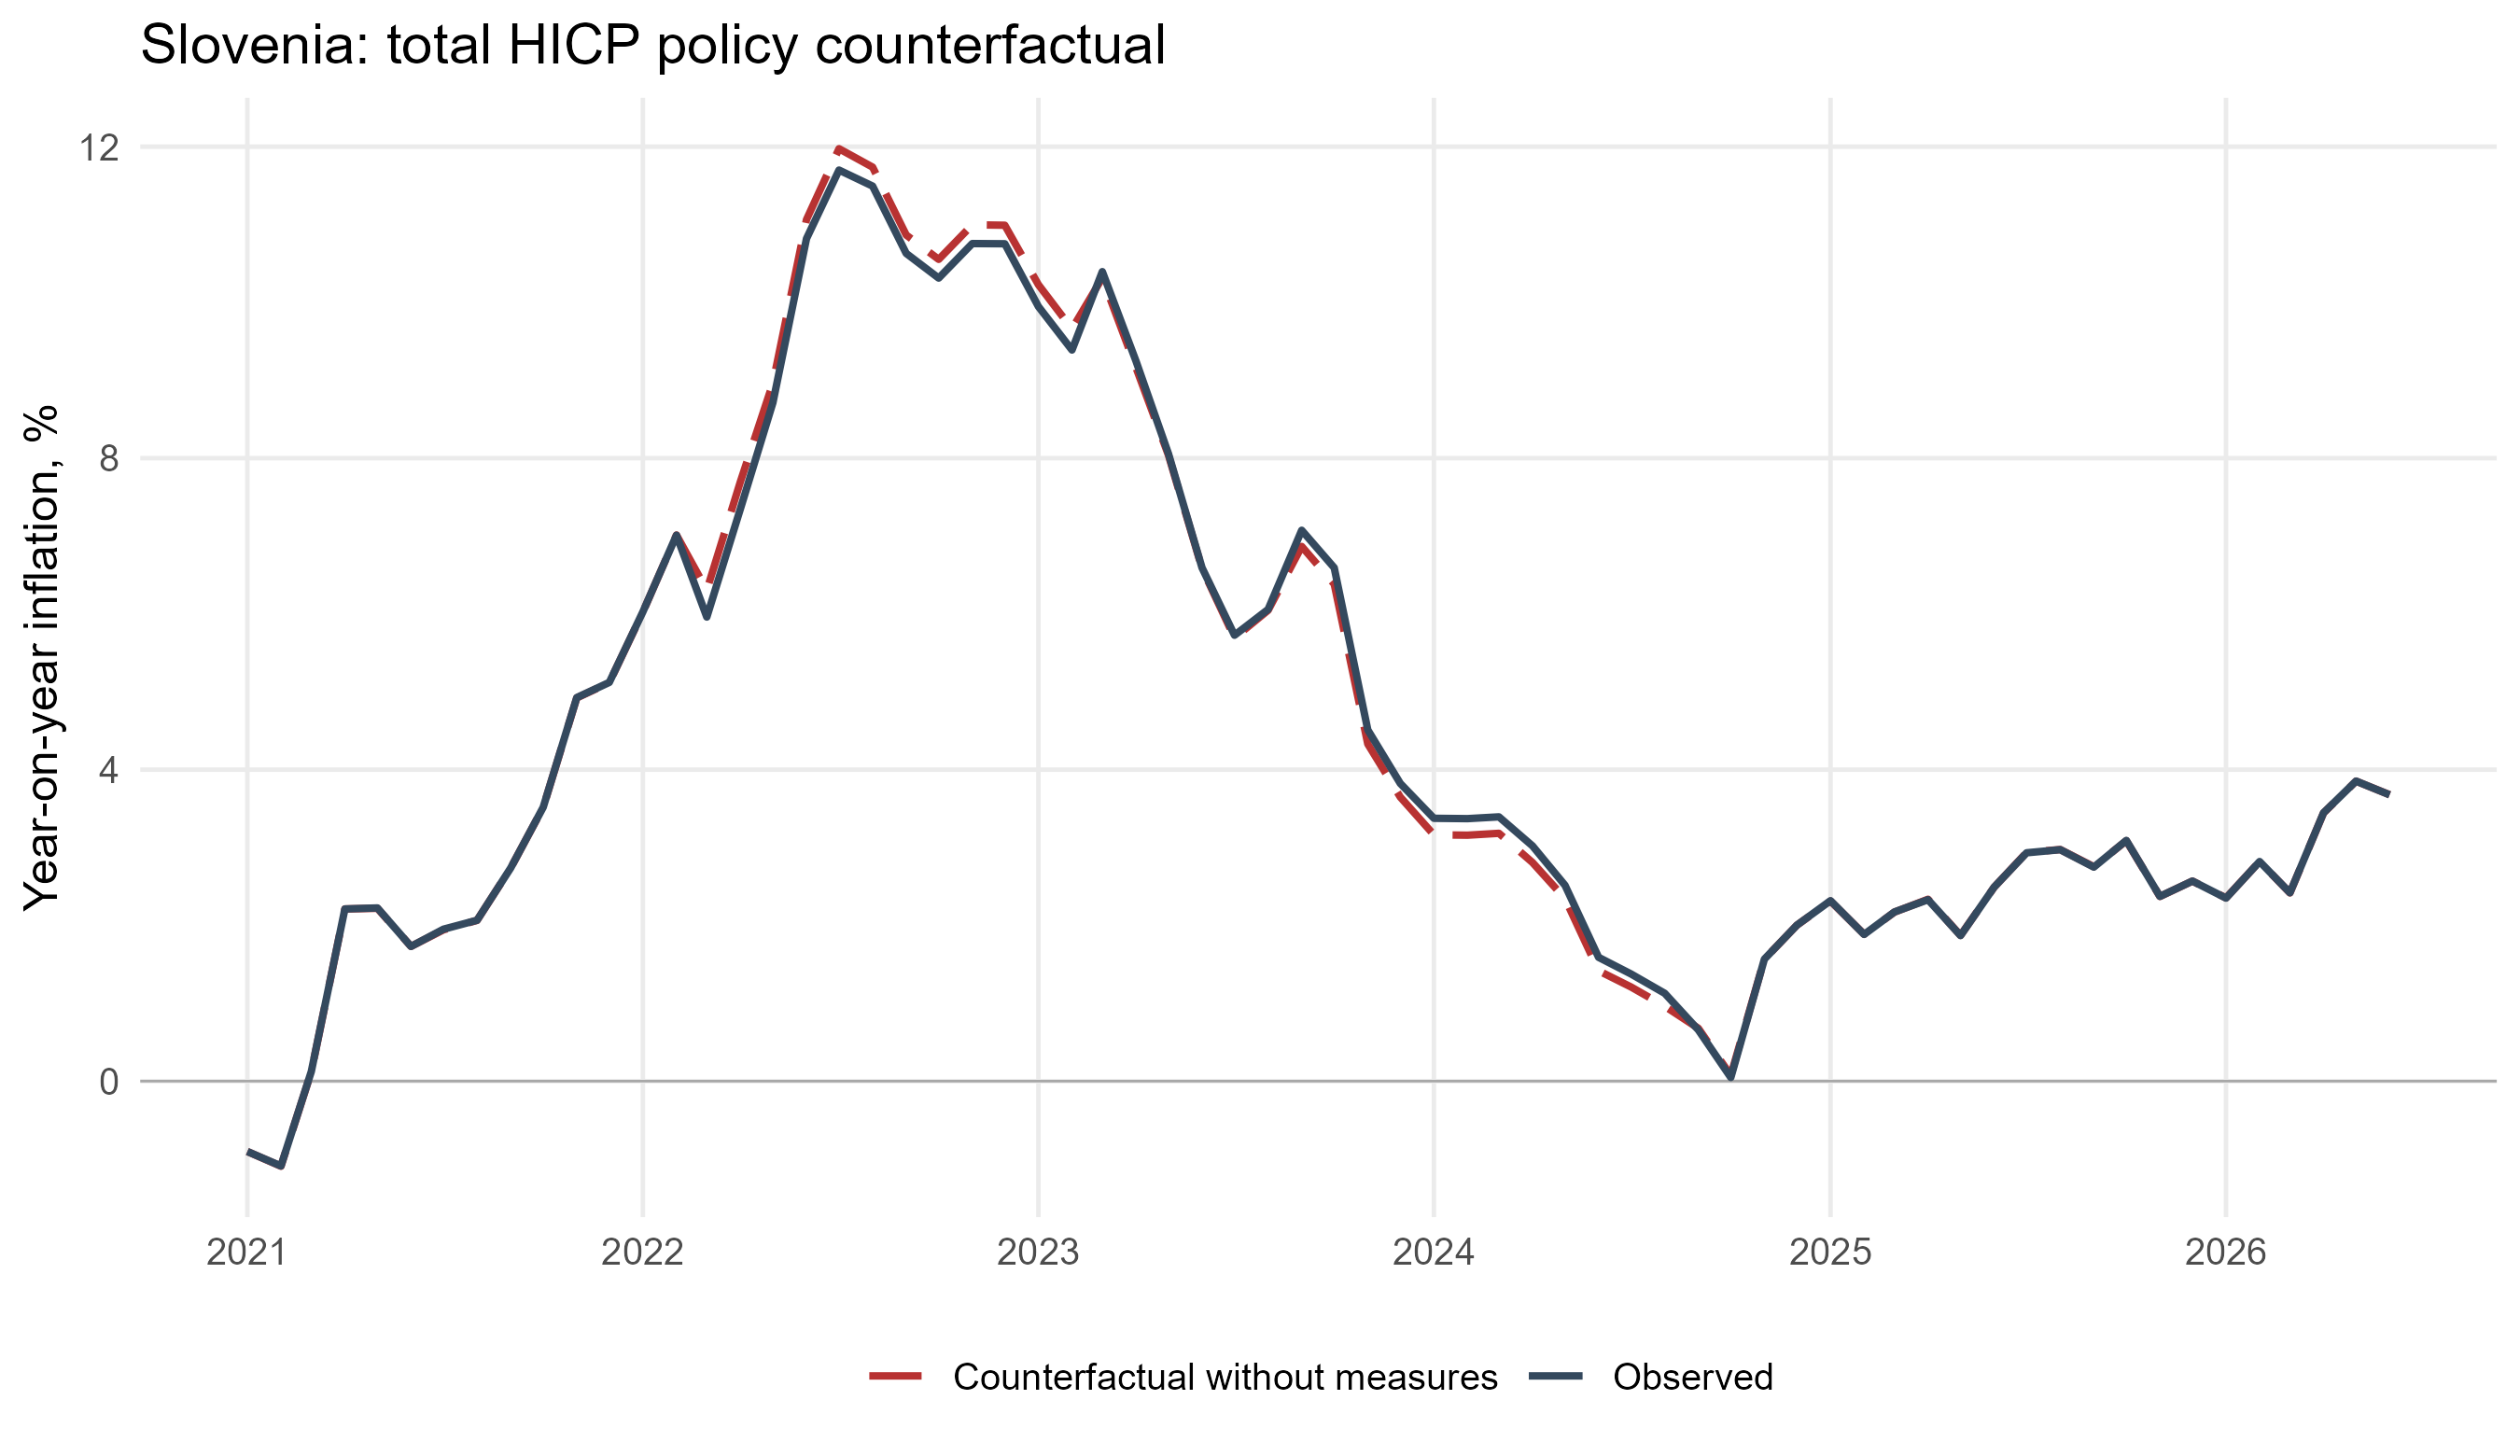
\includegraphics[width=0.86\textwidth,height=0.38\textheight,keepaspectratio]{fig/policy_total_cpi_counterfactual_inflation_SI_slovenia.png}
\caption{Slovenia: observed and counterfactual inflation}
\end{figure}



% Auto-generated from data/counterfactual_measure_assumptions.xlsx (include = TRUE).
\begin{landscape}
\scriptsize
\setlength{\LTleft}{0pt}
\setlength{\LTright}{0pt}
\setlength{\tabcolsep}{2pt}
\renewcommand{\arraystretch}{1.08}
\captionof{table}{Price measures and assumptions included in the national counterfactual simulations}
\label{tab:ea20-price-counterfactual-measures}
\vspace{0.3em}
\begin{longtable}{@{}p{0.62in}p{2.55in}p{2.15in}p{1.30in}p{2.05in}@{}}
\toprule
Country & Included price measure & Rate cut or retained assumption & Start--end dates & Notes \\
\midrule
\endfirsthead
\toprule
Country & Included price measure & Rate cut or retained assumption & Start--end dates & Notes \\
\midrule
\endhead
\midrule
\multicolumn{5}{r}{\emph{Continued on next page}}\\
\endfoot
\bottomrule
\endlastfoot
Austria & Electricity excise reduced from 1.5 to 0.1 ct/kWh & Calibrated no-policy/observed price ratio: 1.05 (+5\%) & 2022-05-01--2024-12-01 &  \\
Austria & Natural-gas excise reduced from 6.6 to 1.196 ct/m3 & Calibrated no-policy/observed price ratio: 1.045 (+4.5\%) & 2022-05-01--2024-12-01 &  \\
Austria & Electricity cost brake: 10 ct/kWh base price, subsidy capped at 30 ct/kWh for 2,900 kWh & Calibrated no-policy/observed price ratio: 1.48 (+48\%) & 2022-12-01--2024-06-01 & Required tariff microdata unavailable. \\
Austria & Electricity cost brake reduced phase: subsidy capped at 15 ct/kWh for 2,900 kWh & Calibrated no-policy/observed price ratio: 1.24 (+24\%) & 2024-07-01--2024-12-01 &  \\
Belgium & Social energy tariff and basic electricity package & Calibrated no-policy/observed price ratio: 1.1 (+10\%) & 2022-03-01--2023-03-01 & Required tariff microdata unavailable. \\
Belgium & Temporary VAT cut on residential electricity from 21\% to 6\% & Calibrated no-policy/observed price ratio: 1.142 (+14.2\%) & 2022-03-01--2022-12-01 &  \\
Belgium & Social energy tariff and basic gas package & Calibrated no-policy/observed price ratio: 1.15 (+15\%) & 2022-04-01--2023-03-01 & Required tariff microdata unavailable. \\
Belgium & Temporary VAT cut on residential natural gas and district heat from 21\% to 6\% & Calibrated no-policy/observed price ratio: 1.142 (+14.2\%) & 2022-04-01--2022-12-01 &  \\
Croatia & Electricity-price mitigation package & Calibrated no-policy/observed price ratio: 1.122 (+12.2\%) & 2022-04-01--2022-09-01 &  \\
Croatia & Gas VAT cut and household price subsidy & Calibrated no-policy/observed price ratio: 1.504 (+50.4\%) & 2022-04-01--2023-03-01 & Specified to avoid double counting. \\
Croatia & VAT cut from 13\% to 5\% on eligible fresh food products & Calibrated no-policy/observed price ratio: 1.04 (+4\%) & 2022-04-01--2023-12-01 & Category coverage is partial. \\
Croatia & District-heating price freeze & Calibrated no-policy/observed price ratio: 1.2 (+20\%) & 2022-10-01--2023-03-01 &  \\
Croatia & Household electricity price cap & Calibrated no-policy/observed price ratio: 1.3 (+30\%) & 2022-10-01--2023-03-01 & Required tariff microdata unavailable. \\
Cyprus & Electricity cost subsidy after VAT reduction & Calibrated no-policy/observed price ratio: 1.12 (+12\%) & 2022-09-01--2023-02-01 & Required tariff microdata unavailable. \\
Estonia & 50\% reimbursement of electricity network fees & Calibrated no-policy/observed price ratio: 1.1 (+10\%) & 2021-10-01--2022-03-01 & Relief applies to one bill component. \\
Estonia & 100\% reimbursement of household gas network fees & Calibrated no-policy/observed price ratio: 1.15 (+15\%) & 2021-12-01--2022-03-01 &  \\
Estonia & 65\% compensation of district-heating increase above October 2021 tariff & Calibrated no-policy/observed price ratio: 1.2 (+20\%) & 2022-02-01--2022-03-01 & Tariffs vary across municipalities. \\
Estonia & Household electricity price compensation & Calibrated no-policy/observed price ratio: 1.2 (+20\%) & 2022-10-01--2023-03-01 & Budget evidence does not identify prices. \\
Estonia & Household natural-gas price compensation & Calibrated no-policy/observed price ratio: 1.2 (+20\%) & 2022-10-01--2023-03-01 &  \\
Finland & Temporary 7.5 percentage-point reduction in the biofuel distribution obligation & Calibrated no-policy/observed price ratio: 1.03 (+3\%) & 2022-05-01--2023-12-01 & Budget evidence does not identify prices. \\
Finland & Temporary electricity VAT reduction from 24\% to 10\% & Calibrated no-policy/observed price ratio: 1.127 (+12.7\%) & 2023-01-01--2023-04-01 &  \\
France & Gas tariff freeze and subsequent gas price cap & Monthly source trajectory; scalar fallback ratio: 1.2 (+20\%) & 2021-11-01--2023-12-01 & Monthly trajectory used; scalar is fallback. \\
France & Regulated electricity tariff cap and TICFE/TCCFE reduction & Monthly source trajectory; scalar fallback ratio: 1.15 (+15\%) & 2022-02-01--2023-12-01 & Monthly trajectory used; scalar is fallback. \\
France & Transport-fuel rebate of 18 then 30 cents per litre & Monthly source trajectory; scalar fallback ratio: 1.12 (+12\%) & 2022-03-01--2022-12-01 & Monthly trajectory used; scalar is fallback. \\
Germany & Early abolition of the EEG electricity levy (3.723 ct/kWh to zero) & Statutory no-policy/observed price ratio: 1.103 (+10.3\%) & 2022-07-01--2022-12-01 & Assumes full pass-through. \\
Germany & Temporary VAT cut on natural gas from 19\% to 7\% & Statutory no-policy/observed price ratio: 1.112 (+11.2\%) & 2022-10-01--2024-03-01 & Assumes full pass-through. \\
Germany & Gas price brake & Calibrated no-policy/observed price ratio: 1.2 (+20\%) & 2023-01-01--2023-12-01 & Required tariff microdata unavailable. \\
Germany & Household electricity price brake: EUR 0.40/kWh on 80\% of reference consumption & Calibrated no-policy/observed price ratio: 1.1 (+10\%) & 2023-01-01--2023-12-01 & Required tariff microdata unavailable. \\
Greece & Electricity consumption subsidy for households & Calibrated no-policy/observed price ratio: 1.35 (+35\%) & 2021-09-01--2023-12-01 & Aggregate proxy; no micro-simulation. \\
Greece & Natural-gas consumption subsidy for households & Calibrated no-policy/observed price ratio: 1.2 (+20\%) & 2021-10-01--2022-12-01 & Eligibility is approximated. \\
Greece & Direct subsidy on automotive diesel & Calibrated no-policy/observed price ratio: 1.08 (+8\%) & 2022-04-01--2022-09-01 & Cash transfers excluded from HICP prices. \\
Ireland & Temporary excise-duty cuts on petrol and diesel & Calibrated no-policy/observed price ratio: 1.1 (+10\%) & 2022-03-01--2023-02-01 &  \\
Ireland & Electricity Costs Emergency Benefit Scheme credits & Calibrated no-policy/observed price ratio: 1.08 (+8\%) & 2022-04-01--2023-03-01 & Credit is per bill, not per kWh. \\
Ireland & Temporary VAT cut on electricity from 13.5\% to 9\% & Calibrated no-policy/observed price ratio: 1.041 (+4.1\%) & 2022-05-01--2023-02-01 &  \\
Ireland & Temporary VAT cut on gas from 13.5\% to 9\% & Calibrated no-policy/observed price ratio: 1.041 (+4.1\%) & 2022-05-01--2023-02-01 &  \\
Ireland & Public Service Obligation levy reduction & Calibrated no-policy/observed price ratio: 1.03 (+3\%) & 2022-10-01--2023-09-01 &  \\
Italy & Electricity general system charges removed & Calibrated no-policy/observed price ratio: 1.09 (+9\%) & 2021-10-01--2023-03-01 & Aggregate proxy; no micro-simulation. \\
Italy & Gas general system charges removed or reduced & Calibrated no-policy/observed price ratio: 1.029 (+2.9\%) & 2021-10-01--2023-12-01 & Specified to avoid double counting. \\
Italy & Strengthened social bonus on electricity bills & Calibrated no-policy/observed price ratio: 1.02 (+2\%) & 2021-10-01--2023-12-01 & Targeted benefit; coverage approximated. \\
Italy & Strengthened social bonus on natural-gas bills & Calibrated no-policy/observed price ratio: 1.02 (+2\%) & 2021-10-01--2023-12-01 & Targeted benefit; coverage approximated. \\
Italy & Temporary 5\% VAT rate on household natural gas & Calibrated no-policy/observed price ratio: 1.122 (+12.2\%) & 2021-10-01--2023-12-01 & Aggregate proxy; no micro-simulation. \\
Italy & Temporary excise-duty cuts on petrol and diesel & Calibrated no-policy/observed price ratio: 1.15 (+15\%) & 2022-03-01--2022-11-01 &  \\
Latvia & Removal of OIK and electricity network charges & Calibrated no-policy/observed price ratio: 1.62 (+62\%) & 2022-01-01--2022-04-01 & Aggregate proxy; no micro-simulation. \\
Latvia & Natural-gas heating compensation of EUR 30/MWh & Calibrated no-policy/observed price ratio: 1.2 (+20\%) & 2022-07-01--2023-04-01 & Eligibility is approximated. \\
Latvia & Compensation of 50\% of district-heating tariff above EUR 68/MWh & Calibrated no-policy/observed price ratio: 1.2 (+20\%) & 2022-10-01--2023-04-01 & Tariffs vary across municipalities. \\
Lithuania & Compensation of household electricity prices & Calibrated no-policy/observed price ratio: 1.25 (+25\%) & 2022-07-01--2023-06-01 & Budget evidence does not identify prices. \\
Lithuania & Partial subsidy on household natural-gas prices & Calibrated no-policy/observed price ratio: 1.3 (+30\%) & 2022-07-01--2023-06-01 & Universal household coverage. \\
Luxembourg & Energiedësch electricity-price stabilisation & Calibrated no-policy/observed price ratio: 1.03 (+3\%) & 2022-02-01--2022-12-01 & Required tariff microdata unavailable. \\
Luxembourg & Energiedësch gas-network-fee subsidy & Calibrated no-policy/observed price ratio: 1.05 (+5\%) & 2022-02-01--2022-09-01 &  \\
Luxembourg & Temporary reduction of 7.5 euro cents per litre of motor fuel & Calibrated no-policy/observed price ratio: 1.045 (+4.5\%) & 2022-04-01--2022-08-01 & Aggregate proxy; no micro-simulation. \\
Luxembourg & Natural-gas increase limited to 15\% and state coverage of network costs & Calibrated no-policy/observed price ratio: 1.15 (+15\%) & 2022-10-01--2024-12-01 & Required tariff microdata unavailable. \\
Luxembourg & Residential electricity-price stabilisation at the 2022 level & Calibrated no-policy/observed price ratio: 1.15 (+15\%) & 2023-01-01--2024-12-01 & Required tariff microdata unavailable. \\
Malta & Government subsidy keeping household electricity tariffs stable & Calibrated no-policy/observed price ratio: 1.3 (+30\%) & 2022-01-01--2023-12-01 & Budget evidence does not identify prices. \\
Malta & Government subsidy stabilising petrol and diesel retail prices & Calibrated no-policy/observed price ratio: 1.15 (+15\%) & 2022-01-01--2023-12-01 & Aggregate proxy; no micro-simulation. \\
Netherlands & Temporary 21\% cut in petrol and diesel excise duties & Calibrated no-policy/observed price ratio: 1.08 (+8\%) & 2022-04-01--2022-12-01 &  \\
Netherlands & Temporary VAT cut on energy from 21\% to 9\% - electricity & Calibrated no-policy/observed price ratio: 1.11 (+11\%) & 2022-07-01--2022-12-01 &  \\
Netherlands & Temporary VAT cut on energy from 21\% to 9\% - gas & Calibrated no-policy/observed price ratio: 1.11 (+11\%) & 2022-07-01--2022-12-01 &  \\
Netherlands & Electricity price cap EUR 0.40 per kWh up to 2900 kWh & Calibrated no-policy/observed price ratio: 1.25 (+25\%) & 2023-01-01--2023-12-01 & Required tariff microdata unavailable. \\
Netherlands & Gas price cap EUR 1.45 per m3 up to 1200 m3 & Calibrated no-policy/observed price ratio: 1.35 (+35\%) & 2023-01-01--2023-12-01 & Required tariff microdata unavailable. \\
Portugal & ISP and carbon-tax reductions on petrol and diesel & Calibrated no-policy/observed price ratio: 1.1 (+10\%) & 2022-05-01--2023-12-01 &  \\
Portugal & Electricity VAT reduction from 13\% to 6\% & Calibrated no-policy/observed price ratio: 1.066 (+6.6\%) & 2022-10-01--2023-12-01 &  \\
Portugal & Bread and cereals zero-VAT basket & Statutory no-policy/observed price ratio: 1.06 (+6\%) & 2023-04-01--2023-12-01 &  \\
Portugal & Fish zero-VAT basket & Statutory no-policy/observed price ratio: 1.06 (+6\%) & 2023-04-01--2023-12-01 &  \\
Portugal & Fruit zero-VAT basket & Statutory no-policy/observed price ratio: 1.06 (+6\%) & 2023-04-01--2023-12-01 &  \\
Portugal & Meat zero-VAT basket & Statutory no-policy/observed price ratio: 1.06 (+6\%) & 2023-04-01--2023-12-01 &  \\
Portugal & Milk cheese and eggs zero-VAT basket & Statutory no-policy/observed price ratio: 1.06 (+6\%) & 2023-04-01--2023-12-01 &  \\
Portugal & Oils and fats VAT measures & Statutory no-policy/observed price ratio: 1.117 (+11.7\%) & 2023-04-01--2026-04-01 & Rates vary across statutory subperiods. \\
Portugal & Plant-based drinks VAT measure & Statutory no-policy/observed price ratio: 1.06 (+6\%) & 2023-04-01--2023-12-01 &  \\
Portugal & Vegetables zero-VAT basket & Statutory no-policy/observed price ratio: 1.06 (+6\%) & 2023-04-01--2023-12-01 &  \\
Slovakia & Flat household electricity commodity, distribution and system charges & Calibrated no-policy/observed price ratio: 1.3 (+30\%) & 2023-01-01--2023-12-01 &  \\
Slovakia & Household heat price cap & Calibrated no-policy/observed price ratio: 1.25 (+25\%) & 2023-01-01--2023-12-01 & Required tariff microdata unavailable. \\
Slovakia & Household natural-gas price cap & Calibrated no-policy/observed price ratio: 1.5 (+50\%) & 2023-01-01--2023-12-01 & Budget evidence does not identify prices. \\
Slovenia & Temporary exemption from electricity network charges & Calibrated no-policy/observed price ratio: 1.1 (+10\%) & 2022-03-01--2022-04-01 & Relief applies to one bill component. \\
Slovenia & Temporary exemption from natural-gas network charges & Calibrated no-policy/observed price ratio: 1.08 (+8\%) & 2022-03-01--2022-04-01 & Relief applies to one bill component. \\
Slovenia & Temporary regulated petrol and diesel retail prices & Calibrated no-policy/observed price ratio: 1.1 (+10\%) & 2022-03-01--2022-08-01 &  \\
Slovenia & Household electricity price cap & Calibrated no-policy/observed price ratio: 1.15 (+15\%) & 2022-09-01--2023-08-01 & Required tariff microdata unavailable. \\
Slovenia & Household natural-gas price cap & Calibrated no-policy/observed price ratio: 1.18 (+18\%) & 2022-09-01--2023-08-01 & Required tariff microdata unavailable. \\
Slovenia & District-heating price cap & Calibrated no-policy/observed price ratio: 1.12 (+12\%) & 2023-01-01--2023-04-01 & Required tariff microdata unavailable. \\
Spain & Electricity VAT reduced from 21\% to 10\% & Calibrated no-policy/observed price ratio: 1.1 (+10\%) & 2021-06-01--2022-06-01 & Eligibility is approximated. \\
Spain & Electricity excise duty reduced from 5.11\% to 0.5\% & Calibrated no-policy/observed price ratio: 1.046 (+4.6\%) & 2021-09-01--2023-12-01 &  \\
Spain & EUR 0.20 per litre petrol and diesel discount & Calibrated no-policy/observed price ratio: 1.11 (+11\%) & 2022-04-01--2022-12-01 &  \\
Spain & Iberian mechanism limiting gas input costs in electricity generation & Calibrated no-policy/observed price ratio: 1.2 (+20\%) & 2022-05-01--2023-12-01 & Aggregate proxy; no micro-simulation. \\
Spain & Electricity VAT reduced from 21\% to 5\% & Calibrated no-policy/observed price ratio: 1.152 (+15.2\%) & 2022-07-01--2023-12-01 & Aggregate proxy; no micro-simulation. \\
Spain & Natural-gas VAT reduced from 21\% to 5\% & Calibrated no-policy/observed price ratio: 1.152 (+15.2\%) & 2022-10-01--2023-12-01 &  \\
Spain & Bread and bread flour VAT reduction & Statutory no-policy/observed price ratio: 1.04 (+4\%) & 2023-01-01--2024-12-01 & Rates vary across statutory subperiods. \\
Spain & Fresh fruit VAT reduction & Statutory no-policy/observed price ratio: 1.04 (+4\%) & 2023-01-01--2024-12-01 & Rates vary across statutory subperiods. \\
Spain & Fresh vegetables and pulses VAT reduction & Statutory no-policy/observed price ratio: 1.04 (+4\%) & 2023-01-01--2024-12-01 & Rates vary across statutory subperiods. \\
Spain & Milk cheese and eggs VAT reduction & Statutory no-policy/observed price ratio: 1.04 (+4\%) & 2023-01-01--2024-12-01 & Rates vary across statutory subperiods. \\
Spain & Olive oil and other edible oils VAT reduction & Statutory no-policy/observed price ratio: 1.074 (+7.4\%) & 2023-01-01--2026-04-01 & Rates vary across statutory subperiods. \\
\end{longtable}
\par\vspace{0.35em}\footnotesize\noindent \emph{Notes:} Each row corresponds to a unique measure marked \texttt{include = TRUE} in \texttt{counterfactual\_measure\_assumptions.xlsx}. Ratios report the counterfactual no-policy price divided by the observed policy-inclusive price. \emph{Statutory} denotes a tax or charge inversion based on the legislated rate; \emph{Calibrated} denotes an aggregate-equivalent price assumption. Where a monthly source trajectory is available, it is used in preference to the displayed scalar fallback. \emph{Sources:} Authors' assumptions workbook and calculations.
\end{landscape}


\end{document}


